\NeedsTeXFormat{LaTeX2e}[1996/06/01]
\documentclass[cup6a]{cupbook}

\usepackage{alltt}
\usepackage{amsfonts}
\usepackage{amsmath}
\usepackage{amssymb}
\usepackage{boxedminipage}
\usepackage{eurosym}
\usepackage{float}
\usepackage{geometry}
\geometry{left=1in,right=1.75in,top=1.25in,bottom=1.25in}
\usepackage{graphicx}
\usepackage{lscape}
\usepackage{makeidx}
\usepackage{multicol}
\usepackage{natbib}
\usepackage{rotating}
\usepackage{scalefnt}
\usepackage{setspace}
\usepackage{hhline}
\usepackage{color}
\usepackage{url}
\usepackage{paralist}
\usepackage{epic}

%  NEEDED ONLY FOR CHAPTER 21
%  HIT RETURN TWICE
\usepackage{subfig}
\captionsetup[subfloat]{justification=raggedright}
\usepackage{caption}
\usepackage[margin=10pt,font=small,labelfont=bf]{caption}

\newcommand{\marginparjed}[1]
{\marginpar{\renewcommand{\baselinestretch}{0.6}\normalsize\raggedright\textit{\footnotesize
#1}}}

\newcommand{\linejed}
{\noindent
\rule{5.5in}{.008in}\vspace{-.15in}\newline\rule{5.5in}{.008in}}

\newcommand{\linetjed}
{\noindent
\rule{5.5in}{.008in}\vspace{-.1in}\newline\rule{5.5in}{.008in}}

\newcommand{\boxedjed}
{\begin{boxedminipage}{5.25in}}

\newcommand\ecaptionjed[1]
  {\addcontentsline{xmp}{example}{#1}}
  \makeatletter \newcommand\listofexamples
  {\section*{Examples}\@starttoc{xmp}}
  \newcommand\l@example[2]
  {\par\noindent#1,~\textit{#2}\par} \makeatother

\newcommand{\empexjed}[1]
{ \marginparjed{\newline \newline \circledR
\scalefont{0.90}{\textsc{ \textbf{Empirical}} \newline Filename is
\newline ``#1''}\scalefont{1.1111}}}

\title{Regression Modeling with Actuarial and Financial Applications}

\author{Edward W. Frees}
\date{\today}
\makeindex

\begin{document}
\setlength{\marginparwidth}{1in}
\setlength{\marginparsep}{0.25in}


\pagenumbering{roman} \maketitle

\pagenumbering{arabic}

\tableofcontents

\input{Chapter20ReportWriting/Chap20_RptWriting02May2009.tex}
\setcounter{chapter}{20}

\chapter{Designing Effective Graphs}\label{c21:ChapGraphs}

{\small \textit{Chapter Preview}.\footnote{This chapter is based on
``Designing Effective Graphs,'' by Edward W. Frees and Robert B.
Miller, 1990, \textit{North American Actuarial Journal}, volume 2,
number 2, 53-70. Published by the Society of Actuaries - reprinted
with permission.} Actuaries, like other business professionals,
communicate quantitative ideas graphically. Because the process of
reading, or decoding, graphs is more complex than reading text,
graphs are vulnerable to abuse. To underscore this vulnerability, we
give several examples of commonly encountered graphs that mislead
and hide information. To help creators design more effective graphs
and to help viewers recognize misleading graphs, this chapter
summarizes guidelines for designing graphs that show important
numerical information. When designing graphs, creators should:

(1) Avoid chartjunk

(2) Use small multiples to promote comparisons and assess change

(3) Use complex graphs to portray complex patterns

(4) Relate graph size to information content

(5) Use graphical forms that promote comparisons

(6) Integrate graphs and text

(7) Demonstrate an important message

(8) Know the audience.

Some of these guidelines for designing effective graphs, such as
(6), (7) and (8), are drawn directly from principles for effective
writing. Others, such as guidelines (3), (4) and (5), come from
cognitive psychology, the science of perception. Guidelines (1) and
(2) have roots both in effective writing and in graphical
perception. For example, the writing principle of brevity
demonstrates how eliminating pseudo three-dimensional perspectives
and other forms of chartjunk improve graphs. As another example, the
writing principle of parallel structure suggests using small
multiple variations of a basic graphical form to visualize complex
relationships across different groups and over time.


To underscore the scientific aspect of graphical perception, we
examine the process of communicating with a graph, beginning with a
sender's interpretation of data and ending with a receiver's
interpretation of the graph. In keeping with scientific tradition,
this chapter discusses several studies in the literature on the
effectiveness of graphs.

We conclude that the actuarial profession has many opportunities to
improve its practice, making communication more efficient and
precise.}


\section{Introduction}\label{S21:Intro}

Like other business professionals, actuaries communicate ideas
orally and in writing, as well as through presentations, which are
interactive forms of communication that encompass oral and written
messages. Actuaries, as well as other financial analysts,
communicate ideas with important quantitative components. Writers
express quantitative ideas as (1) numbers within paragraphs, (2)
numbers within tabular forms, (3) functional relationships such as
equations, and (4) data or equations as graphs.

Graphs are a simple yet powerful medium for written communication of
quantitative ideas. Graphs can present a large amount of data in a
small space, express important relationships between quantities,
compare different sets of data, and describe data, thus providing a
coherent picture of complex systems. Graphs do more than merely
state an idea; they demonstrate it.

Graphs are powerful because they are flexible, but flexibility can
be a disadvantage because of the potential for abuse. Well-accepted
references dealing with methods of quantitative data presentation
mitigate opportunities for abuse. The \emph{Chicago Manual of Style}
(1993), a standard reference, discusses presentation of in-text
data, and Ehrenberg (1977) and Tufte (1983) discuss presentation of
tabular data. In contrast, we focus on data presentation through
\emph{graphical} displays.

This chapter seeks to improve actuarial practice as it relates to
graphical displays. We intend to: (1) demonstrate the importance of
graphical displays, (2) provide guidelines to improve graphical
practice, and (3) introduce some of the scientific underpinnings of
good graphical practice. The agenda is ambitious, yet the goal of
this chapter is to provide practicing actuaries with basic tools
that they can use to become critical consumers and effective
producers of graphs. We also hope that readers will adopt our
enthusiasm and wish to explore the graphical design literature on
their own.

An important theme of this chapter is that principles of vigorous
writing can and should be applied to the practice of making
effective graphs. The \emph{Elements of Style} (Strunk and White
1979, p. xiv) summarizes vigorous writing:

\marginparjed{``\ldots sixty-three words that could change the
world.''}

\smallskip \boxedjed

Vigorous writing is concise. A sentence should contain no
unnecessary words, a paragraph no unnecessary sentences, for the
same reason that a drawing should have no unnecessary lines and a
machine no unnecessary parts. This requires not that the writer make
all his sentences short, or that he avoid all detail and treat his
subjects only in outline, but that every word tell.

\end{boxedminipage}

\smallskip

White attributes this quotation to William Strunk. White calls it
``a short, valuable essay on the nature and beauty of
brevity--sixty-three words that could change the world.'' We argue
that brevity is especially important when making effective graphs.
This was also understood by Strunk; as noted above, he said ``a
drawing should contain no unnecessary lines \ldots'' We use the term
\emph{chartjunk}, introduced by Tufte (1983), for any unnecessary
appendage in a graph.\index{plots!chartjunk}


\marginparjed{Chartjunk is any unnecessary appendage in a graph.}

Vigorous writing principles other than brevity also apply to the
practice of making effective graphs. Just as with writing, effective
graphs are the result of repeated revising and editing. Poorly
designed graphs can and do hide information and mislead. Fancy or
pretentious graphs are distracting when simpler graphs suffice.


Although the principles of effective writing are valuable, they are
not sufficient for producing effective graphs. Writing is processed
in a serial manner, word by word, sentence by sentence, with a
beginning and an ending. The process of ``reading,'' or
\emph{decoding}, a graph is nonlinear and more complex. The
additional complexities mean that even authors who follow effective
writing practices may produce ineffective graphs. Often the form of
written prose is the sole determinant of its value, whereas in
graphics the communication process plays the dominant role. We
assume that readers are familiar with effective writing forms. Thus,
we first review the communication process in which a graph plays a
crucial role.

To underscore the importance of effective graphical design, Section
\ref{S21:GDesign} provides several illustrations of graphs that hide
information and are misleading; the defects illustrated are more
serious drawbacks than mere chartjunk. The Section \ref{S21:GDesign}
illustrations motivate the need for additional guidelines and
methods for constructing effective graphs.

Section \ref{S21:DesignGuide} introduces eight important guidelines
for creating and viewing graphs. Although the guidelines do not
provide a panacea for all graphical defects, they do provide
business professionals such as actuaries with a key checklist for
creating effective graphs. The guidelines are organized so that the
first two, on chartjunk and the use of multiples, are based on both
effective writing and graphical perception perspectives. Guidelines
Three, Four and Five are related primarily to the graphical
perception literature, whereas Guidelines Six, Seven and Eight are
based primarily on effective writing principles.

As with effective writing, questions of style enter into the
discussion of what is and what is not an effective graph. Many style
decisions are based upon accepted practices without a firm
scientific foundation. However, the process of perceiving graphs has
been the subject of inquiry in several scientific disciplines,
including psychophysics, cognitive psychology, and computational
visions (Cleveland 1995, Chapter 4). Section
\ref{S21:EmpiricalFoundations} illustrates some types of
experimental evidence for determining an effective graphical form
based on both the receiver and the graph itself as units of study.
Section \ref{S21:EmpiricalFoundations} also illustrates how such
mainstays of business publications as bar charts and pie charts are
poor communicators of numerical information.

Sections \ref{S21:Conclude} and {S21:References} contain concluding
remarks and descriptions of some resources for actuaries who wish to
learn more about designing effective graphs.

Most readers are removed from the detailed data summarized by a
graph. Several difficulties and misconceptions can arise owing to
the distance between the original data and a viewer's interpretation
of the graph. Figure \ref{F21:Flowchart} illustrates the challenge
of communicating with a graph. The sender (and creator) of the graph
has a message derived from an interpretation of data. Although a few
graphs communicate raw data, the primary purpose of most graphs is
to communicate the sender's interpretation. The message the sender
intends is encoded in a graph and passed on to the receiver.

\begin{figure}[htp]
  \begin{center}
    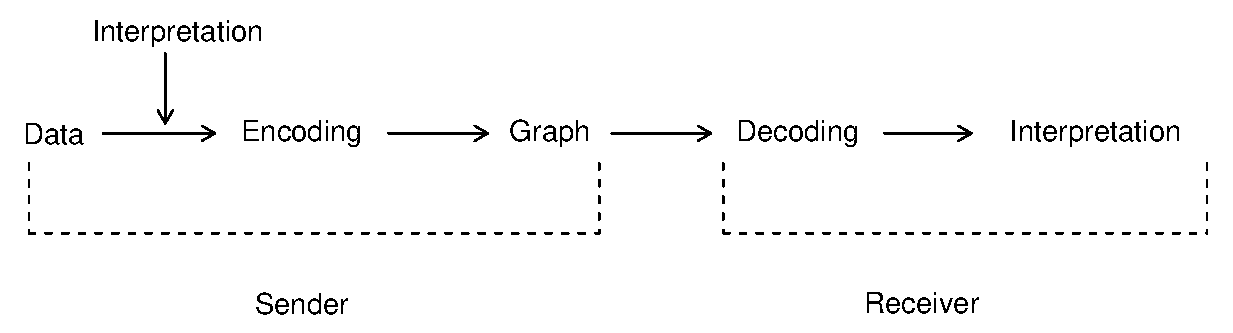
\includegraphics[width=.8\textwidth]
        {Chapter21Graphs/Fig21_1FlowChart.eps}
    \caption{\label{F21:Flowchart} \small Flow Chart of the Process of
Communicating with a Graph. The graph is a crucial intermediary in
the process of communicating data interpretation to the receiver.}
  \end{center}
\end{figure}

In general, the receiver is party to neither the exact
interpretation intended by the sender nor the raw data. Thus the
receiver must decode the graph and develop an interpretation of its
message. Two issues arise:
\begin{itemize}
\item Whether the interpretation constructed
by the receiver is congruent to the interpretation of the sender

\item Whether the receiver's
interpretation is consistent with and supported by the data.

\end{itemize}

The first issue depends on the skill with which the sender
constructs the graph and the skill with which the receiver decodes
it. A poorly constructed graph can hide or distort the sender's
message. A graph that is hard to read can discourage the receiver
from spending the time necessary to decode the message correctly.
The receiver can ignore or misinterpret a graph that is not
constructed with care.

The second issue depends not only on the skills mentioned above but
also on the skill with which the sender draws meaning from the data.
How carefully does the sender document the process of
interpretation? Is this communicated to the receiver? Is the
receiver capable of assessing the extent to which the graph is a
credible summary of the data? Failure at any of these points could
result in the receiver ignoring or misinterpreting the graph.

This chapter assumes that the graphs included in business
communications are the subject of scrutiny by serious readers.
Graphs that appear quickly on the television screen, a flip chart or
presentation package are designed to attract attention and to
entertain the viewer. Design, rather than information,
considerations dominate these media. We focus instead on graphs that
are part of professional writing and are designed to inform. As with
effective writing, we assume that in creating graphs ``\ldots one
must believe - in the truth and worth of the scrawl, in the ability
of the reader to receive and decode the message'' (Strunk and White
1979, p. 84). We now turn to examples of graphs that mislead.

\section{Graphic Design Choices Make a Difference}\label{S21:GDesign}

As noted by Schmid (1992), the ancient proverb ``One picture is
worth ten thousand words,'' when applied to graphs might well read,
``One picture \emph{can be} worth ten thousand words \emph{or
figures}.'' Graphic potential is not easily realized. Because of
their flexibility, graphs too easily render visual displays of
quantitative information that are uninformative, confusing or even
misleading.

Examples \ref{S21:GDesign}.1 through \ref{S21:GDesign}.5 illustrate
five different types of deceptive graphs. In each case, the data
were not altered nor were different dimensions of the data
portrayed. The common theme of the examples is that, by altering
only the data scales, the creator can alter dramatically a viewer's
interpretation.

\linejed

\textbf{Example \ref{S21:GDesign}.1: Including Zero To Compress
Data}. Figure \ref{F21:InsurEmploy} shows a time series of the
percentage of full-time equivalent workers employed in the insurance
industry. The annual data, 1948-1993, are from the National Income
and Product Accounts produced by the Bureau of Labor Statistics. The
left-hand panel, Figure \ref{F21:InsurEmploy}(a), provides the
impression of a stable employment environment for the insurance
industry. Including zero on the vertical axis produces this seeming
stability. By doing this, most of the graph is devoted to white
space that does not show the variability in the data. In contrast,
the right-hand panel, Figure \ref{F21:InsurEmploy}(b), uses the data
to set the range on the axes. This panel clearly shows the large
employment increases in the years following the Korean War, circa
1952. It also allows the reader to see the employment declines that
the insurance industry has suffered in the most recent three years.

\begin{figure}[htp]
  \begin{center}\subfloat[\textbf{A stable insurance
industry}]{
   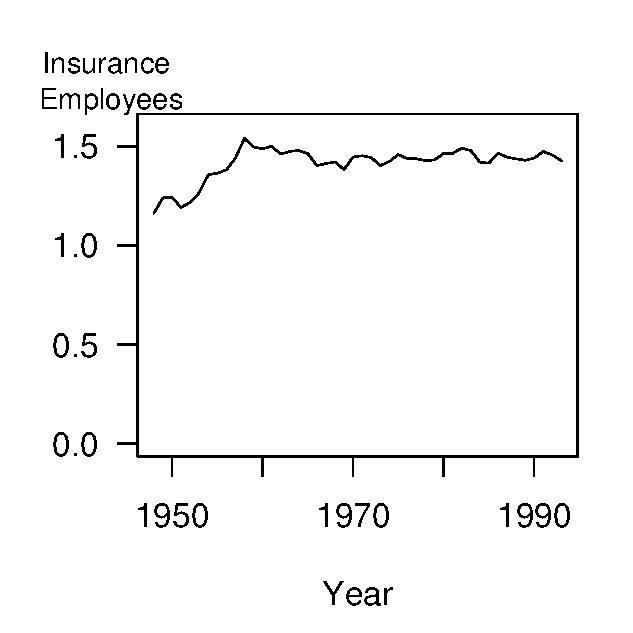
\includegraphics[width=0.45\textwidth]
   {Chapter21Graphs/Fig21_2InsurEmploya.eps}}  \hfill
   \subfloat[\textbf{The insurance industry work force increased
dramatically in the 1950s}]{
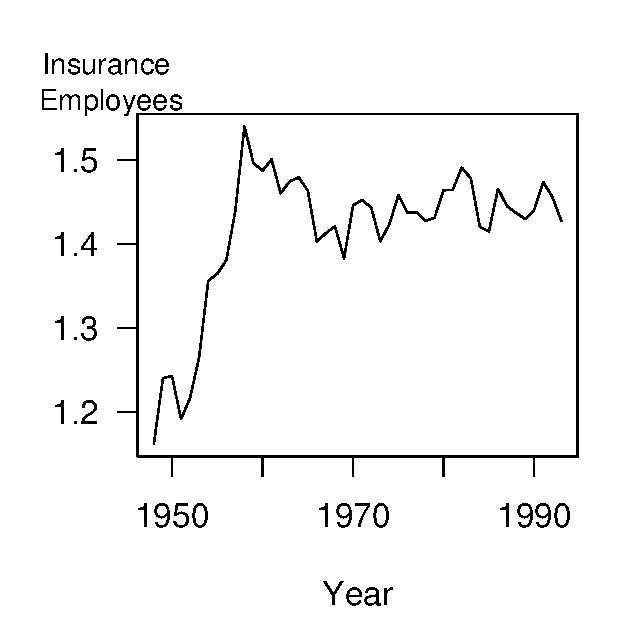
\includegraphics[width=0.45\textwidth]
        {Chapter21Graphs/Fig21_2InsurEmployb.eps}}
    \caption{\label{F21:InsurEmploy} \small Annual Insurance Employees, 1948-1993. ``Insurance employees'' is
the percentage of full-time-equivalent employees who are working for
insurance carriers. Allowing the data to determine the scale ranges
reveals interesting aspects of the data.}
  \end{center}
\end{figure}

This example is similar to a popular illustration from Huff's
well-known \emph{How to Lie with Statistics} (Huff 1954). The point
is that motivation external to the data, such as including zero on
an axis, can invite us to alter the data scale and change a viewer's
interpretation of the data. As Example \ref{S21:GDesign}.2 shows,
creators of graphs can also alter a viewer's interpretation by
changing both scales of a two-dimensional graph.

\empexjed{RiskSurvey}\index{datasets!risk managers cost
effectiveness}

\linejed

\textbf{Example \ref{S21:GDesign}.2: Perception of Correlation}.
Figure \ref{F21:FirmRMcostvsSize} relates risk management cost
effectiveness to firm size. These data are from a survey of 73 risk
managers of large, U.S.-based, international firms that was
originally reported in Schmit and Roth (1990). The data are analyzed
in Section 6.5. Here, the measure of risk management cost
effectiveness, firm cost, is defined to be the logarithm of the
firm's total property and casualty premiums and uninsured losses as
a percentage of total assets. The firm size measure is total assets
in logarithmic units.


\begin{figure}[htp]
  \begin{center}\subfloat[\textbf{The data in this figure appear
 less correlated}]{
   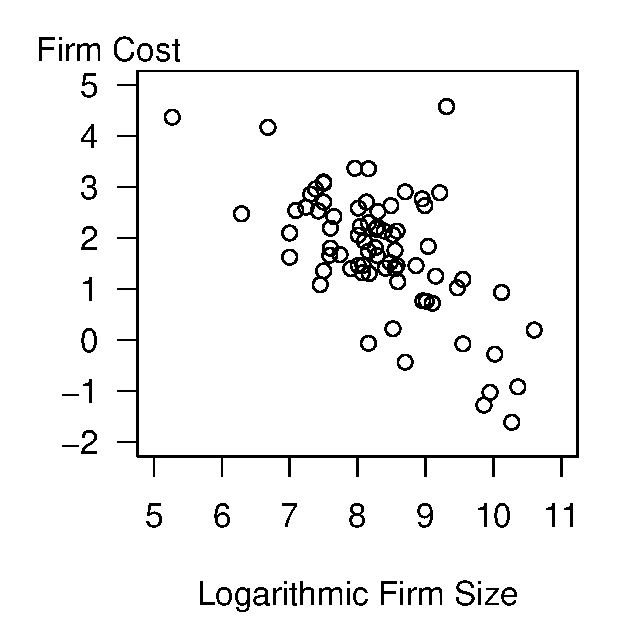
\includegraphics[width=0.45\textwidth]
   {Chapter21Graphs/Fig21_3FirmRMcostvsSizea.eps}}  \hfill
   \subfloat[\textbf{The data in this figure appear
more correlated}]{
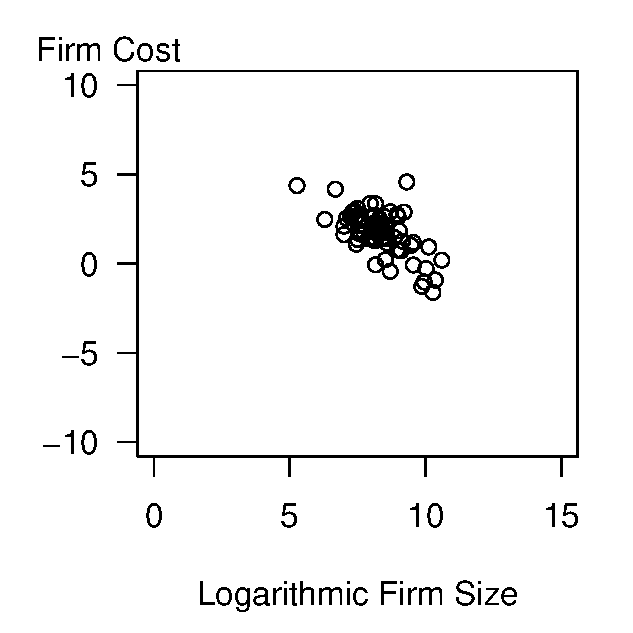
\includegraphics[width=0.45\textwidth]
        {Chapter21Graphs/Fig21_3FirmRMcostvsSizeb.eps}}
    \caption{\label{F21:FirmRMcostvsSize} \small Cost
Effectiveness of a Firm's Risk Management Practices Versus Firm
Size. The data represented in each figure are the same. However, the
wider scales in panel (b) suggest that the data are more highly
correlated.}
  \end{center}
\end{figure}


The left-hand panel, Figure \ref{F21:FirmRMcostvsSize}(a), shows a
negative relationship between firm costs and firm size, as
anticipated by Schmit and Roth. The correlation coefficient between
the two variables is -0.64. The data are in a small center portion
of Figure \ref{F21:FirmRMcostvsSize}(b) when compared to the
left-hand panel, Figure \ref{F21:FirmRMcostvsSize}(a). Figure
\ref{F21:FirmRMcostvsSize}(a) uses the data to determine the axes
and thus shows more patterns in the data. As Cleveland, Diaconis,
and McGill (1982) show, the scaling makes the data in the right-hand
panel appear more correlated than in the left-hand panel.

Change of scales can also alter the viewer's perception of trend in
time series data, as illustrated in Example \ref{S21:GDesign}.3.

\linejed

\textbf{Example \ref{S21:GDesign}.3: Transforming to a Logarithmic
Scale}. Figure \ref{F21:InsurInForce} exhibits a time series of the
U.S. credit insurance market over 1950-1989. These data are analyzed
in Frees (1996) and are originally from the \emph{Life Insurance
Fact Book} (1990). When the amount of insurance is examined on a
linear scale in Figure \ref{F21:InsurInForce}(a), the credit
insurance market appears to be expanding rapidly. However, Figure
\ref{F21:InsurInForce}(b) shows that, when examined on a logarithmic
scale, the market is leveling off. As discussed in Section 3.2.2,
changes on a logarithmic scale can be interpreted as proportional
changes. Thus, Figure \ref{F21:InsurInForce}(a) shows the market is
increasing rapidly, and Figure \ref{F21:InsurInForce}(b) shows that
the rate of increase is leveling off. These messages are not
contradictory, but viewers must interpret each graph critically to
understand the intended message.

\begin{figure}[htp]
  \begin{center}\subfloat[\textbf{U.S. credit life insurance market exploding}]{
   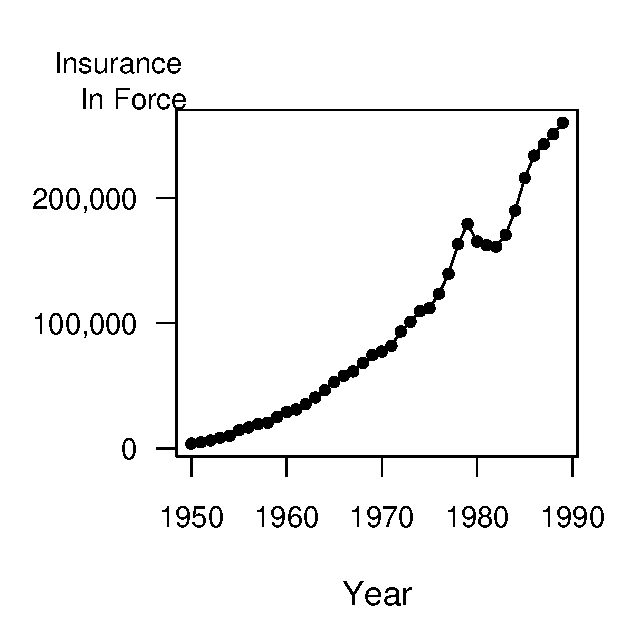
\includegraphics[width=0.45\textwidth]
   {Chapter21Graphs/Fig21_4InsurInForcea.eps}}  \hfill
   \subfloat[\textbf{U.S. credit life insurance market leveling
off}]{
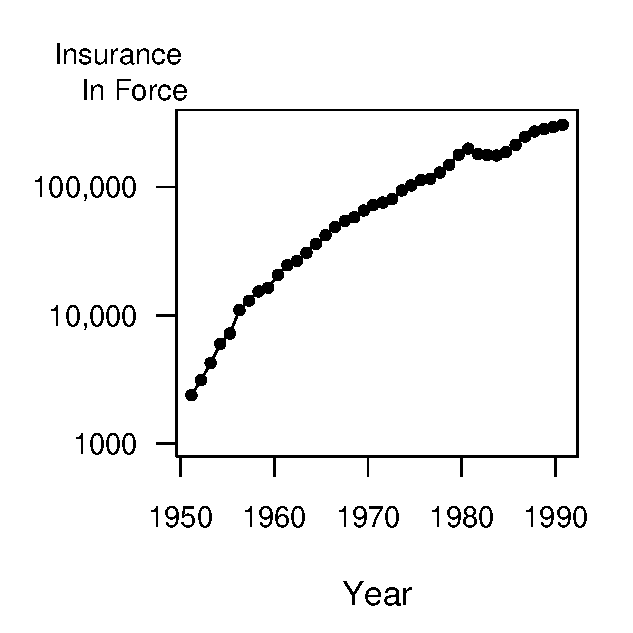
\includegraphics[width=0.45\textwidth]
        {Chapter21Graphs/Fig21_4InsurInForceb.eps}}
    \caption{\label{F21:InsurInForce} \small Annual U.S. Credit Life Insurance in Force, 1950-1989. Different
vertical scales give different impressions of the rate of growth
over time.}
  \end{center}
\end{figure}

\newpage


\linejed

\textbf{Example \ref{S21:GDesign}.4: Double Y-Axes}. Figure
\ref{F21:CPI} displays two measures of inflation that are produced
by the Bureau of Labor Statistics. On the left-hand axes are CPI\_U,
the consumer price index for urban consumers. On the right-hand axes
are CPI\_M, the consumer price index for medical components of the
overall index. Each series consists of monthly values ranging from
January 1947 through April 1995.

\begin{figure}[htp]
  \begin{center}\subfloat[\textbf{Overall Consumer Price Index (CPI) is similar to
the medical component of the CPI}]{
   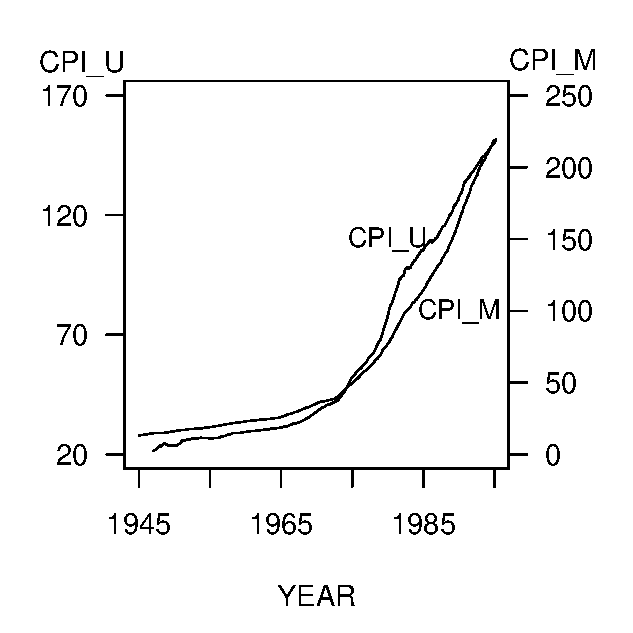
\includegraphics[width=0.45\textwidth]
   {Chapter21Graphs/Fig21_5CPIa.eps}}  \hfill
   \subfloat[\textbf{Overall Consumer Price Index
(CPI) is increasing more slowly than the medical component of the
CPI}]{
\includegraphics[width=0.45\textwidth]
        {Chapter21Graphs/Fig21_5CPIb.eps}}
    \caption{\label{F21:CPI} \small Monthly Values of the Overall Consumer Price Index (CPI) and the
Medical Component of the CPI, January 1947 through April 1995.
Different scale ranges alter the appearances of relative growth of
the two series.}
  \end{center}
\end{figure}


The left-hand panel, Figure \ref{F21:CPI}(a), suggests that the
CPI\_U and the CPI\_M begin and end in approximately the same
position, thus implying that they have increased at about the same
rate over the period. The creator could argue that each index
measures the value of a standard bundle of goods, thus justifying
the argument for using a different scale for each series.

The right-hand panel, Figure \ref{F21:CPI}(b), provides a more
useful representation of the data by using the same scale for each
series. Here, CPI\_M begins lower than CPI\_U and ends higher. That
is, the medical component index has increased more quickly than the
index of prices for urban consumers. Other patterns are also evident
in Figure \ref{F21:CPI}: each series increased at roughly the same
rate over 1979-1983 and CPI\_M increased much more quickly from 1983
to 1994 when compared to 1948-1979.

\linejed

\textbf{Example \ref{S21:GDesign}.5: Aspect Ratio}. Figure
\ref{F21:tsUnemploy} shows a time series plot of the monthly
unemployment rate, April 1953 through December 1992. The
unemployment rate is the percentage of unemployed civilian labor
force, seasonally adjusted. It is part of the Household Survey
produced by the Bureau of Labor Statistics, Department of Labor.
This series was analyzed in Frees et al. (1997). The top panel of
Figure \ref{F21:tsUnemploy} shows that the unemployment rate
averaged 5.9\% with a peak of 10.8\% in the fourth quarter of 1982
and a minimum of 2.7\% in the third quarter of 1953.

\begin{figure}[htp]
  \begin{center}
    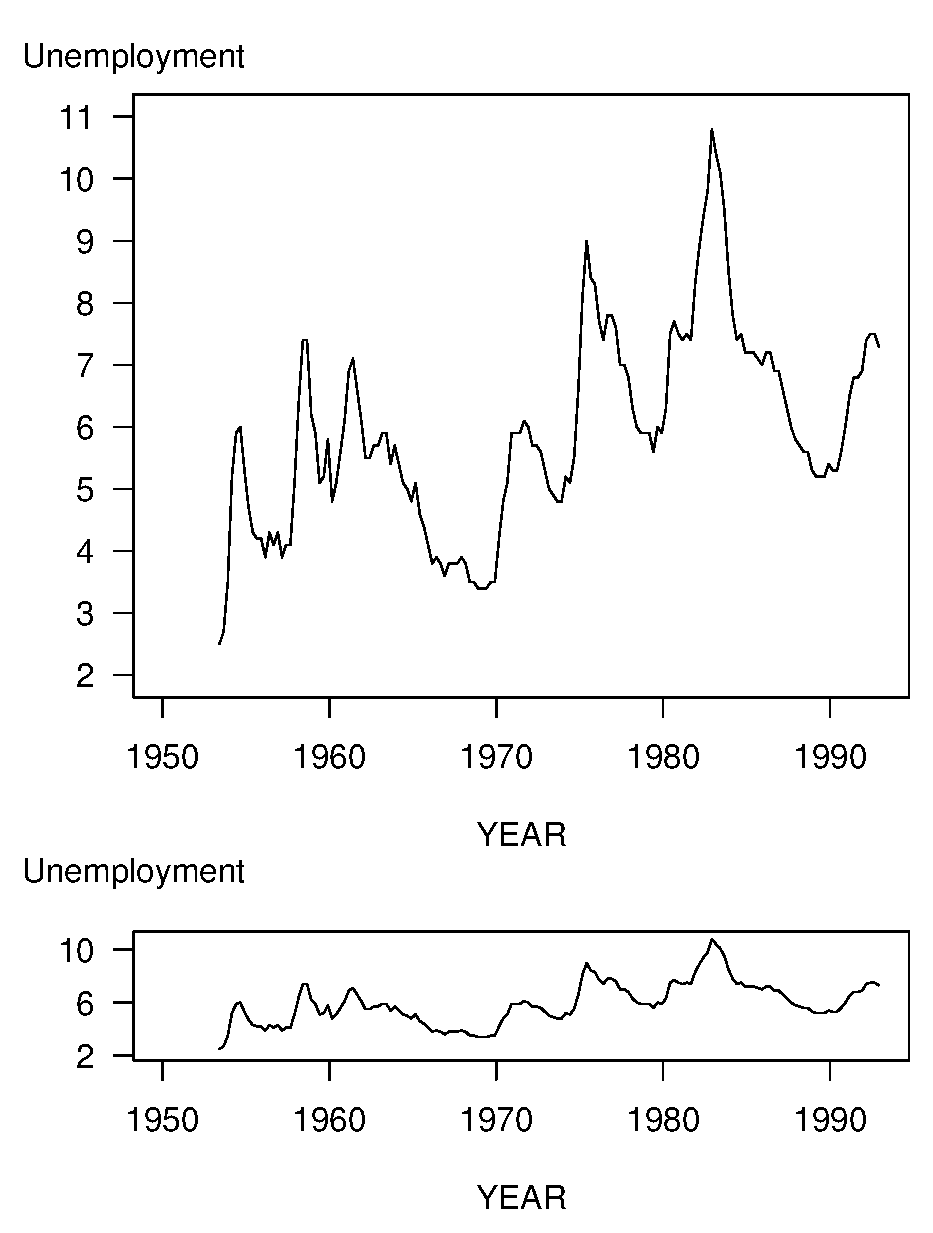
\includegraphics[width=0.45\textwidth]
        {Chapter21Graphs/Fig21_6tsUnemploy.eps}
    \caption{\label{F21:tsUnemploy} \small Time Series Plot of Quarterly Values of the U.S. Unemployment Rate,
1953-1992. The lower panel displays a feature that is not evident in
the upper panel; unemployment declines more slowly than it rises.}
  \end{center}
\end{figure}


The two panels in Figure \ref{F21:tsUnemploy} differ only in their
shape, not in the scaling of either variable or in the relative
amount of space that the data take within the figure frame. To
differentiate these two shapes, we can use the concept of a figure's
\emph{aspect ratio}, defined to be the height of the data frame
divided by its width (some sources use the reciprocal of this value
for the aspect ratio). The data frame is simply a rectangle whose
height and width just allow the graph \emph{of the data} to fit
inside. To illustrate, in the upper panel in Figure
\ref{F21:tsUnemploy}, the length of the vertical side is equal to
the length of the horizontal side. In the lower panel, the vertical
side is only 25\% of the horizontal side.

\marginparjed{A figure's aspect ratio is defined to be the height of
the data frame divided by its width.}\index{plots!aspect ratio}

Both panels show that the unemployment series oscillated widely over
this 39-year period. The lower panel, however, displays a feature
that is not apparent in the upper panel; the rise to the peak of an
unemployment cycle is steeper than the descent from the peak. Within
each unemployment cycle, the percentage of workers unemployed tends
to rise quickly to a maximum and then to fall gradually to a
minimum. This behavior is surprisingly regular over the almost
39-year period displayed in the plot.

Different aspect ratios can leave substantially different
impressions on the eye, as Figure \ref{F21:tsUnemploy} illustrates.
Thus, the aspect ratio can be chosen to emphasize different features
of the data.

\linejed

\section{Design Guidelines}\label{S21:DesignGuide}

Understanding the issues illustrated in Section \ref{S21:GDesign}
can help actuaries and other business professionals create and
interpret graphs. This section presents eight guidelines for
designing effective graphs. One of our main points is that current
practice is not in accord with these guidelines. Thus, we anticipate
that not all of our readers will find the demonstrations of the
guidelines visually appealing, but, as stated in Section
\ref{S21:Intro}, many of the guidelines are based on a scientific
foundation outlined in Section \ref{S21:EmpiricalFoundations}.
``Intuition'' is something we learn and cultivate; progress in
science does not always conform to current intuition. It was widely
believed at one time that the earth was flat and that the sun
revolved about the earth. The demonstrations of this section may or
may not be immediately intuitive, but they are logical conclusions
from the design guidelines advocated here.

\subsubsection*{Guideline One: Avoid Chartjunk}

In Section \ref{S21:Intro}, we defined chartjunk to be any
unnecessary appendage in a graph. Creators of graphs who use
chartjunk lower their credibility with serious receivers. Even when
senders convey a correct interpretation accompanied by chartjunk,
they ask receivers to process and properly ignore the chartjunk. If
chartjunk is part of the default, or easily used, options of a
software package, then the sender can clutter a graph, or even make
a graph misleading, simply by punching a button.

\marginparjed{Avoid pictures that are not worth ten thousand
words.}\index{plots!chartjunk}

Senders who avoid chartjunk raise their credibility. They ask
receivers to look only at meaningful characters and marks. Senders
may have to spend considerable time with their software to make
effective graphs, but the respect and attention of their receivers
reward them. Another way to avoid chartjunk is not to use a graph at
all if a few words will do. If the message in a graph can be
summarized in a few words, then the graph is not needed. Avoid
pictures that are not worth ten thousand words!

Avoiding chartjunk is based in part on the concept of brevity in
vigorous writing principles. From the graphical perception
viewpoint, avoiding chartjunk reduces the noise when communicating
between the graph's sender and receiver. Thus, this guideline is
important because it has roots in both writing and perception
principles.

\linejed

\textbf{Example \ref{S21:DesignGuide}.1: Premium Receipts of Life
Insurance Companies}. Figure \ref{F21:DotPlotPremiumReceipts}(a) is
an adaptation of a graph on page 69 of the \emph{Life Insurance Fact
Book }(1994). The graph reports 15 bits of information: 5 years and
2 percentages for each year (a third percentage is found by
subtraction). A three-dimensional box represents each percentage,
and each box displays different shadings to represent the three
lines of business: health, annuity and life. These figures could be
reported compactly in a small table. However, granting that a graph
may help the receiver appreciate trends in the figures, the graph's
simplicity should reflect the simplicity of the information
available in the figures. In particular, a small plotting symbol
suffices to report a percentage. A three-dimensional, shaded box is
hardly called for. It is interesting that the three-dimensional box
was an ``innovation'' in 1994. Earlier editions of the \emph{Fact
Book} used two-dimensional boxes. The volume of chartjunk took a big
jump in 1994.

\begin{figure}[htp]
  \begin{center}\subfloat[\textbf{The three-dimensional stacked bar chart
is a poor graphical form for making comparisons over time and across
lines of business}.]{
   \includegraphics[width=0.45\textwidth]
   {Chapter21Graphs/3DBarChartNew.eps}}  \hfill
   \subfloat[\textbf{The dot plot allows for direct comparison over
time and across lines of business.}]{
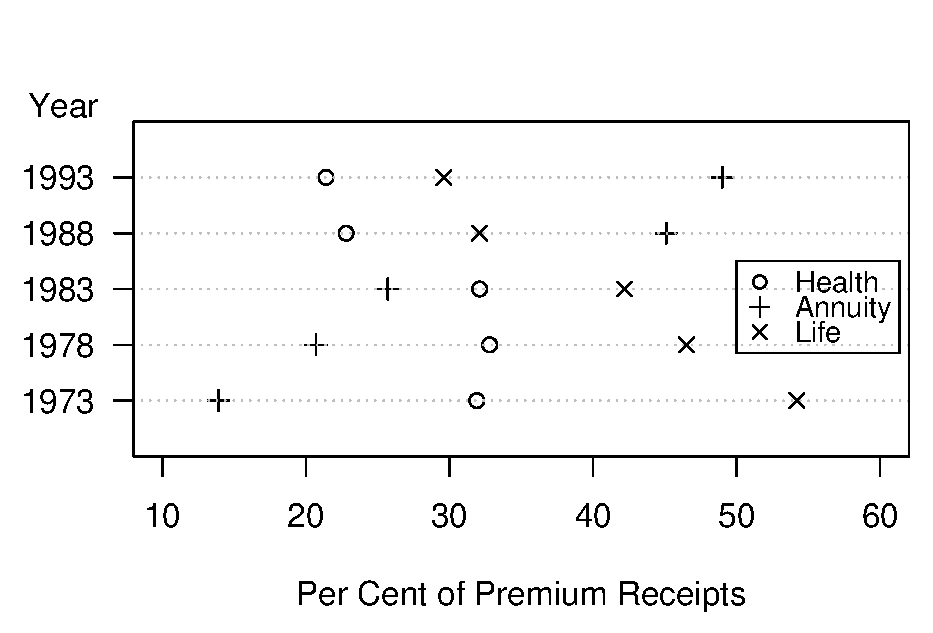
\includegraphics[width=0.45\textwidth]
        {Chapter21Graphs/Fig21_7bDotPlotPremiumReceipts.eps}}
    \caption{\label{F21:DotPlotPremiumReceipts} \small Distribution of Premium Receipts, 1973-1993. The excessive
chartjunk of (a) hides the large change in distribution types
between 1983 and 1988.}
  \end{center}
\end{figure}


Figure \ref{F21:DotPlotPremiumReceipts}(b) is a \emph{dot plot},
discussed by Cleveland (1994). Different plotting symbols show the
different lines of business. The tick marks on the lower horizontal
axes help us estimate the percentages, and the light, dotted grid
lines help us scan across the graph to the plotting symbols of
interest. The major shifts, and the approximate magnitudes of the
shifts, that happened between 1983 and 1988 are clear here.

\linejed

\subsubsection*{Guideline Two: Use Small Multiples to Promote Comparisons and Assess Change}

Statistical thinking is directed towards comparing measurements of
different entities and assessing the change of a measurement over
time or some other unit of measurement. Graphical displays are
inherently limited when portraying comparisons or assessing changes
because they are static, two-dimensional media. Graphs that contain
multiple versions of a basic graphical form, each version portraying
a variation of the basic theme, promote comparisons and assessments
of change. By repeating a basic graphical form, we promote the
process of communication.

Tufte (1997) states that using \emph{small multiples} in graphical
displays achieves the same desirable effects as using parallel
structure in writing. Parallel structure in writing is successful
because it allows readers to identify a sentence relationship only
once and then focus on the meaning of each individual sentence
element, such as a word, phrase or clause. Parallel structure helps
achieve economy of expression and draw together related ideas for
comparison and contrast. Similarly, small multiples in graphs allow
us to visualize complex relationships across different groups and
over time.

\marginparjed{Small multiples in graphs allow us to visualize
complex relationships across different groups and over time.}

The Section \ref{S21:GDesign} figures illustrated the use of small
multiples. In each figure, the two plots portrayed were identical
except for the change in scale; this use of parallel structure
allowed us to demonstrate the importance of scaling when
interpreting graphs. Example \ref{S21:DesignGuide}.2 illustrates
another application of small multiples in graphical displays,
Cleveland's (1993) multiway dot plot.

\linejed

\textbf{Example \ref{S21:DesignGuide}.2: Relative Importance of Risk
Source}. Figure \ref{F21:MultipleDotPlots}, called a \emph{multiway
dot plot}, demonstrates conclusions reached by using a model
introduced in Frees (1998) concerning the relative importance of
risk sources within a block of short-term insurance contracts. The
risk sources are the stochastic interest environment, the frequency
of claims (mortality), and the possibility of a catastrophic event
(disaster) occurring. The relative importance of these three risk
sources is considered by letting two parameters of interest vary.
These parameters are the expected year until disaster and, in the
event of disaster, the expected proportion (probability) of
policyholders that will succumb to disaster.

\begin{figure}[htp]
  \begin{center}
    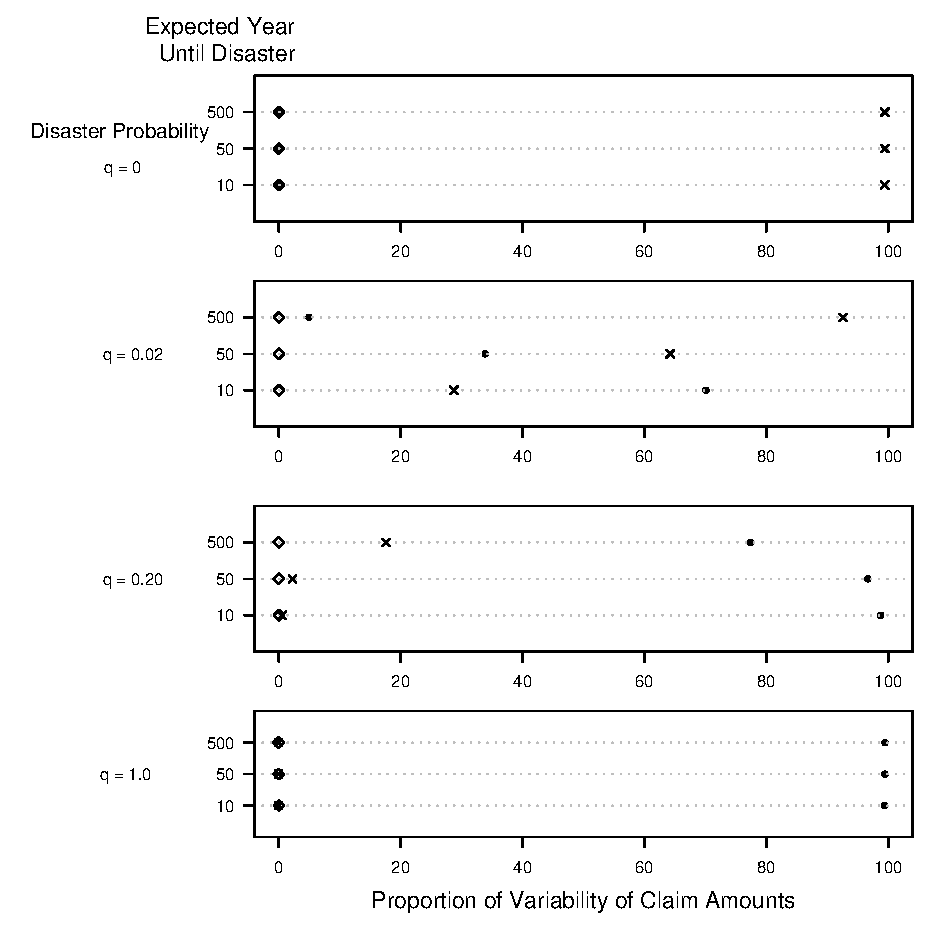
\includegraphics[width=0.8\textwidth]
        {Chapter21Graphs/Fig21_8MultipleDotPlots.eps}
  \includegraphics[width=0.1\textwidth]
        {Chapter21Graphs/Fig21_8Legend.eps}
    \caption{\label{F21:MultipleDotPlots} \small The Relative Importance of Risk Sources. This complex graph allows
us to visualize differences over sources of risk (interest, disaster
and mortality), expected year until disaster, and probability of
disaster. The multiway dot plot demonstrates how quickly the
importance of the disaster component increases as the probability of
disaster increases.}
  \end{center}
\end{figure}

Figure \ref{F21:MultipleDotPlots} shows that when no policyholders
succumb to disaster ($q = 0$), then the frequency component,
mortality, dominates the other risk sources. At the opposite
extreme, when all policyholders succumb to disaster ($q = 1$), then
the disaster component dominates the other risk factors. This is
true even when the expected time until disaster is 500 years! For
the intermediate cases, when either the expected proportion of
policyholders succumbing to disaster increases or the expected year
until disaster decreases, the importance of the disaster component
increases at the expense of the mortality component. Because of the
short-term nature of the contract considered, the interest component
does not play an important role in Figure
\ref{F21:MultipleDotPlots}.

This story of relative importance could not be told using analytic
expressions because of the complexity of the underlying models. The
story behind Figure \ref{F21:MultipleDotPlots} could be told,
however, using tabular displays. The advantage of Figure
\ref{F21:MultipleDotPlots} is that it allows the viewer to make
comparisons over three different risk sources when two parameters of
interest vary. Although such comparisons are possible with tabular
displays, graphical displays are more effective devices.

\linejed

\subsubsection*{Guideline Three: Use Complex Graphs to Portray Complex Patterns}

Many authors believe that a graph should be simple and immediately
understood by the viewer. Simple graphs are desirable because they
can deliver their message to a broad audience and can be shown
quickly and digested immediately. Although this notion may be
appropriate for popular writing, for professional writing the
concept of instant understanding is limiting in that it precludes
the notion that graphs demonstrate complex ideas. Complex patterns
should be portrayed as simply as possible, although the patterns
themselves should not be unnecessarily simplified.

One way for a graph to represent complex patterns is for some of its
basic elements to serve more than one purpose. Tufte (1983) called
such elements \emph{multifunctioning}. For example, we can use
plotting symbols to represent not only elements corresponding to the
horizontal and vertical scales but also a level of a categorical
variable.

\empexjed{WiscHospCosts} \index{datasets!Wisconsin hospital costs}

\linejed\index{actuarial \& financial terms and concepts!health
provider!fee for service, FFS} \index{actuarial \& financial terms
and concepts!health provider!health maintenance organization, HMO}

\textbf{Example \ref{S21:DesignGuide}.3: Frequency and Severity of
Hospital Costs}. Figure \ref{F21:PlotsLogCostDischarge} displays the
relationship between average hospital costs and frequency of
hospital usage. These data for the year 1989 were obtained from the
Office of Health Care Information, Wisconsin's Department of Health
and Human Services, and are further analyzed in Section 4.4. The
data represent averages over the state of Wisconsin, broken down by
nine health service areas, three types of providers (fee for
service, health maintenance organization, and other) and three types
of diagnosis-related groups (DRGs). The three DRGs, numbers 209, 391
and 430, represent major joint and limb reattachment, normal
newborns, and psychoses, respectively. Each plotting symbol in
Figure \ref{F21:PlotsLogCostDischarge} represents a combination of
health service area, type of payer, and type of DRG. The horizontal
axis provides the number of patients admitted in 1989 for each
combination, in natural logarithmic units. The vertical scale
provides the average hospital cost per discharge for each
combination, in natural logarithmic units.

The story in the left-hand panel, Figure
\ref{F21:PlotsLogCostDischarge}(a), is one of increased economies of
scale. That is, combinations of health service areas, type of payer,
and DRG that have a larger number of patients, measured by
discharges, have lower costs. A substantial negative relationship is
evident in Figure \ref{F21:PlotsLogCostDischarge}(a); the
correlation coefficient is -0.43. This is true despite the aberrant
point in the lower left-hand region of Figure
\ref{F21:PlotsLogCostDischarge}(a). The aberrant point is less
important economically than the others; it represents a combination
with only two discharges. When the point is removed, the correlation
becomes -0.50, thus representing an even stronger negative
relationship.

\begin{figure}[htp]
  \begin{center}\subfloat[\textbf{With the exception of one outlying
observation in the lower left-hand region, there appears to be a
significant negative relationship between cost and number of
hospital discharges.}]{
   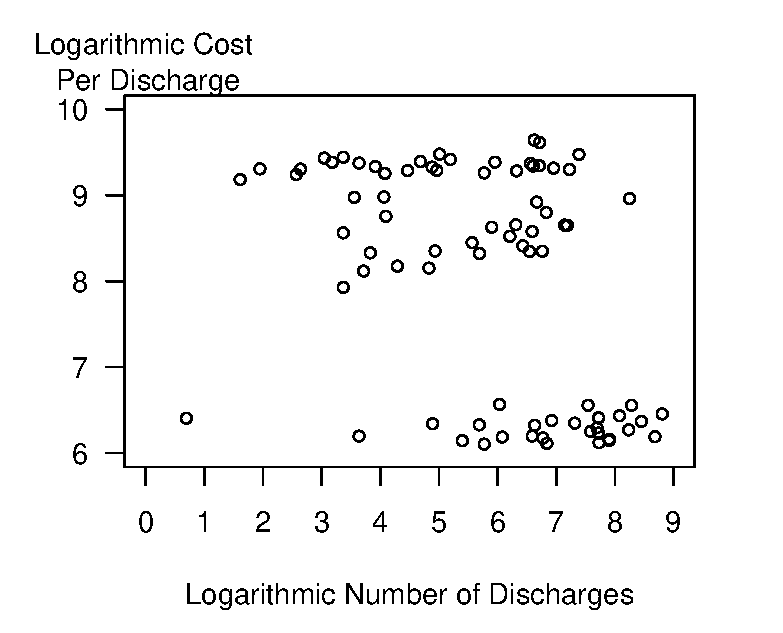
\includegraphics[width=0.45\textwidth]
   {Chapter21Graphs/Fig21_9PlotsLogCostDischargea.eps}}  \hfill
   \subfloat[\textbf{By introducing the DRG codes, we see a
small positive relationship between cost and number of hospital
discharges within each group.}]{
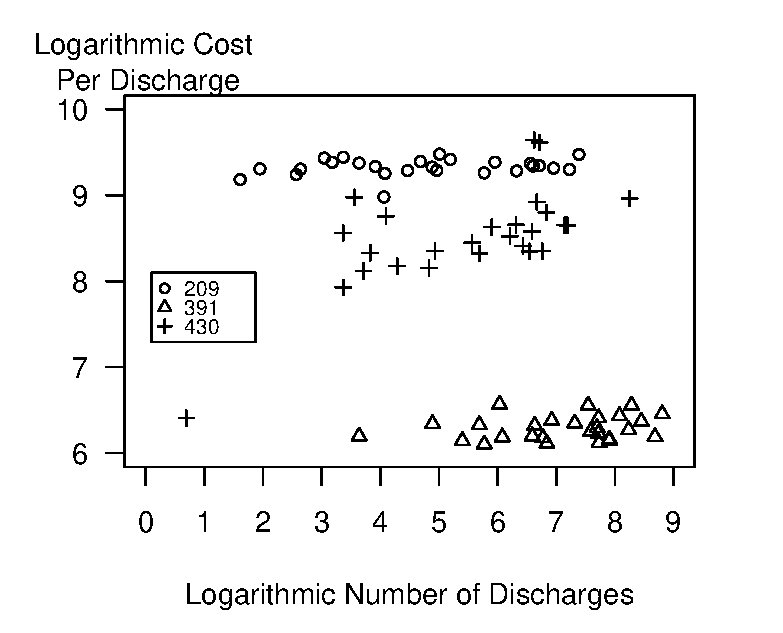
\includegraphics[width=0.45\textwidth]
        {Chapter21Graphs/Fig21_9PlotsLogCostDischargeb.eps}}
    \caption{\label{F21:PlotsLogCostDischarge} \small Logarithmic Cost per Discharge Versus the Logarithmic Number of
Discharges. By adding a plotting symbol code for the level of DRG,
the three distinct groups are evident. The three DRGs, 209, 391, and
430, represent major joint and limb reattachment, normal newborns
and psychoses, respectively.}
  \end{center}
\end{figure}


Despite its simplicity, Figure \ref{F21:PlotsLogCostDischarge}(a)
hides an important relationship. The right-hand panel, Figure
\ref{F21:PlotsLogCostDischarge}(b), is a redrawing of Figure
\ref{F21:PlotsLogCostDischarge}(a) that includes different plotting
symbols for different DRGs. Here, the story is the opposite to the
one of increased economies of scale. For combinations representing
major joint and limb reattachments and normal newborns, the
relationship between frequency and cost is fairly flat. For these
DRGs there are few economies of scale. For the psychoses DRG, number
430, Figure \ref{F21:PlotsLogCostDischarge}(b) shows a small
positive relationship between frequency and cost, even discounting
for the combination with only two patients discharged.

The two panels illustrate a phenomenon in statistics referred to as
\emph{Simpson's paradox}, or a problem of \emph{aggregation of
data}. See Section 4.4 for further discussion. The important point
for this chapter is that sometimes simple graphs are misleading.
Complex graphs may take more time for viewers to interpret, but they
more effectively summarize complex relationships.

\linejed

\subsubsection*{Guideline Four: Relate Graph Size to Information Content}

``How large should the graph be?'' is an important question. The
bounds on size are clear. Graphs should not be so small that they
are not clearly legible, particularly upon reproduction that
degrades an image, nor should they be so large that they exceed a
page. With large graphs, it is difficult to compare elements within
the graph, thus defeating a primary purpose of graphs.

\marginparjed{The data density of a graph is the number of data
entries per unit area of the graph.}\index{plots!data density}

Within these bounds, a graph should be proportional to the amount of
information that it contains. To discuss the proportion of
information content, Tufte (1983) introduced the \emph{data density
of a graph}. This is defined to be the number of data entries per
unit area of the graph. For comparing graph size and information,
the data density is a quantity to be maximized, either by increasing
the number of data entries or reducing the size of the graph. By
examining this density over a number of popular publications, Tufte
concluded that most graphs could be effectively shrunk.

For example, Figure \ref{F21:DotPlotPremiumReceipts}(a) is a chart
with a low data density. This chart represents only 15 numbers. With
an area of approximately 9 square inches, this graph's data density
is roughly 15/9. For comparison, Figure
\ref{F21:InflationWithProjections} shows approximately 600 numbers.
Although Figure \ref{F21:InflationWithProjections}'s area is about
twice as large as that of Figure
\ref{F21:DotPlotPremiumReceipts}(a), the data density is much larger
in Figure \ref{F21:InflationWithProjections} than in Figure
\ref{F21:DotPlotPremiumReceipts}(a).


\begin{figure}[htp]
  \begin{center}
    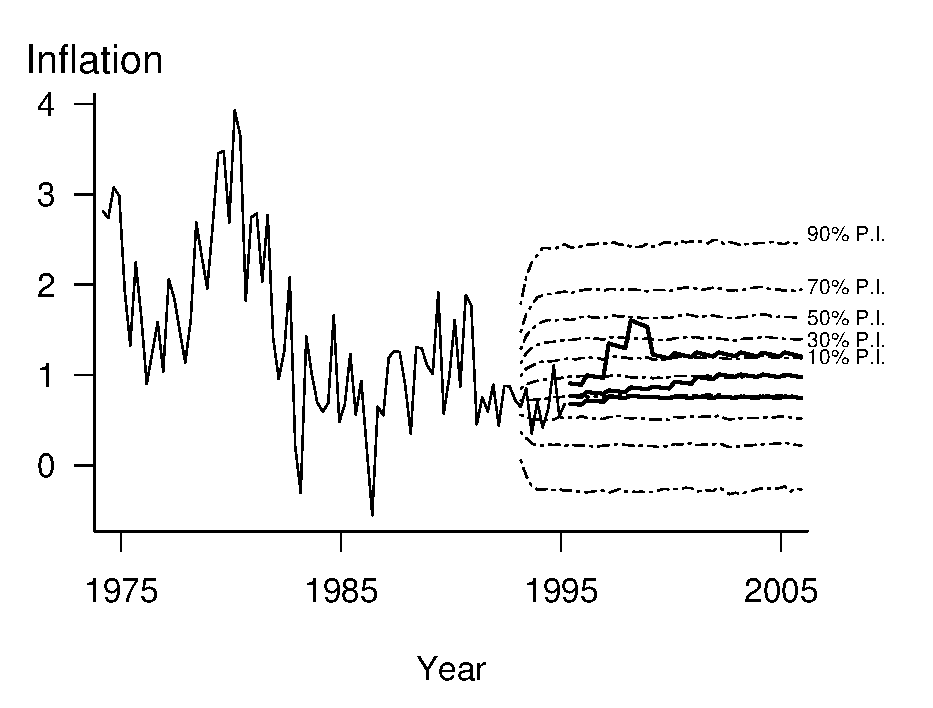
\includegraphics[width=0.9\textwidth]
        {Chapter21Graphs/Fig21_10InflationWithProjections.eps}
    \caption{\label{F21:InflationWithProjections} \small Comparison of Stochastic Prediction Intervals to Held-out Actual
Experience and to Social Security's Assumptions. The thin solid
lines represent actual inflation rates, and the thick solid lines
represent projections by Social Security experts. The dotted lines
represent prediction intervals generated by a stochastic time series
model. This complex graph allows viewers to make comparisons based
on approximately 600 points.}
  \end{center}
\end{figure}

\linejed

\textbf{Example \ref{S21:DesignGuide}.4: Inflation Rate Forecasts}.
Figure \ref{F21:InflationWithProjections} is a complex graph that
contains much information about a complex subject, forecasting the
inflation rate (CPI) for projections of Social Security funds (Frees
et al. 1997). The graph shows actual experience of quarterly
inflation rates up through the first quarter of 1995. Experience up
through 1992 was used to fit a time series model described in Frees
et al. (1997), and this model was used to generate prediction
intervals (PIs) of the inflation rate. These prediction intervals
can be compared to held-out experience that was not used to fit the
model (1993-1995) as well as projections of inflation by Social
Security experts. The thick lines represent high-, intermediate-,
and low-cost inflation projections determined by Social Security
experts.

Figure \ref{F21:InflationWithProjections} is complex and may not be
immediately understood by the viewer. However, almost every stroke
within the data region represents numerical information. Although
complex, Figure \ref{F21:InflationWithProjections} allows the viewer
to compare (1) 20 years of experience to a 10-year forecast, (2)
recent held-out experience to forecasts, and (3) expert projections
to forecasts generated by a time series model. The graph's
complexity reflects the complexity of forecasting inflation rates;
this complexity is not due to unnecessary elements that distract
viewers and make them more ``interested'' in the graph.

\linejed

\subsubsection*{Guideline Five: Use Graphical Forms That Promote Comparisons}

Creators of graphs are often faced with the choice of several
graphical forms that could be used to represent a feature of the
data. As we describe in Guideline Eight, the receiver's knowledge of
graphical forms can influence the choice. Graphical perception is
also an important determinant. In Section
\ref{S21:EmpiricalFoundations}, we discuss this issue in detail. We
include it here as part of the Guidelines Section for completeness.

\subsubsection*{Guideline Six: Integrate Graphs and Text}


Data graphics should be carefully integrated with text, tables, and
other graphs. A legend summarizes the graph and its main message,
but the surrounding text develops the theme leading up to the
message and discusses its impact. Although ``a picture is worth ten
thousand words,'' a graph needs supporting text. Tufte (1983)
encourages readers and writers to think of data graphics as
paragraphs and to treat them as such.

Data graphics can be complemented by a tabular presentation of data:
graphics can highlight relationships among the data, and tables can
present precise numerical descriptions of the data. The two modes
are complementary. A good writing device is to place a graphical
display in the main body of the report and to reinforce the graph
with a tabular display in an appendix.

The American Statistical Association, in its \emph{Style Guide} for
journal publications, reminds us that a detailed legend is helpful
when interpreting graphs. The \emph{Style Guide} recommends that a
legend describe a graph, draw attention to the graph's important
features, and explain this importance.

\subsubsection*{Guideline Seven: Demonstrate an Important Message}

Detailed legends and graphs should reinforce messages that are
developed in the main body of the text. To illustrate, when
considering ways of portraying a complex dataset, choose a graphical
form that highlights an important message. All too often, creators
of graphs display data features that are not part of the theme that
is being developed.

Cleveland (1994) recommends that we ``put major conclusions in a
graphical form.'' In regression data analysis, major conclusions are
about patterns in the data that are summarized using models. Usually
major conclusions are best presented graphically. Graphs display a
large amount of information that is retained by the viewer because
it is visualized. Graphs communicate patterns directly to a viewer,
without using an equation to represent the patterns. In this way, a
wider audience can be reached than if the presentation relies solely
on a model-based interpretation of the data. Further, patterns
suggested by a graph reinforce those represented by a model, and
vice versa. Thus the two tools, graphs and models, reinforce and
strengthen one another.

\marginparjed{``The greatest value of a picture is when it forces us
to notice what we never expected to see.'' Tukey (1977)}

Tukey (1977) states that ``The greatest value of a picture is when
it forces us to notice what we never expected to see.'' Unexpected
phenomena are usually memorable events; viewers of graphs remember
these results, which makes them powerful. In writing this chapter,
we did not expect the results of Figure \ref{F21:tsUnemploy}. This
figure demonstrates that unemployment rises much more quickly than
it declines; it is a powerful example of the use of aspect ratios.

\subsubsection*{Guideline Eight: Know Your Audience}

A basic precept of effective writing, familiarity with one's
audience, is also valid for designing effective graphs. As stated in
the Introduction, our primary motivation in developing guidelines is
to encourage the precise and concise communication of quantitative
ideas to a scientific audience using a written medium. As discussed
in Section \ref{S21:EmpiricalFoundations}, the graphical form is
subservient to the real role of the graphical display,
\emph{communicating} quantitative ideas of the creator to the viewer
of a graph. If the audience does not have an understanding of the
graphical form, then the form will hinder the communication flow
rather than aid it. Thus, each of the seven guidelines already
discussed can be modified or even ignored upon occasion, depending
on the audience for the graph. To illustrate, in Example
\ref{S21:DesignGuide}.1 we argued that the dot plot was superior to
the three-dimensional stacked bar chart. As another example, in
Section \ref{S21:EmpiricalFoundations} we argue that pie charts are
ineffective communicators of information based on the science of
cognitive perception. However, for some audiences, creators of
graphs will prefer the less effective forms based on the level of
audience familiarity. We hope that practice will eventually shift
from these ineffective modes of communication. Still, it is
important to recognize the background of the audience of the graph.
We recommend that creators of graphs not so much swim against the
tide of poor graphic design as bend their course towards more
effective modes of communication.


\section{Empirical Foundations For
Guidelines}\label{S21:EmpiricalFoundations}

This section consists of two different scientific aspects of
graphical studies: science of perception and surveys of graphical
practice.

This chapter does not include a number of graphical forms that are
mainstays in business publications and the popular press, such as
pie charts, pictographs, and stacked bar charts. In fact, we have
shown stacked bar charts in Section \ref{S21:DesignGuide} only as an
example of how \emph{not} to draw figures. Why are these widely used
graphical forms not adopted in an chapter emphasizing data graphics?
The reasons lie in how graphical forms communicate information and
how we perceive graphical information. We demonstrate that, given
how we perceive information, pie and stacked bar charts are poor
communicators of numerical information.

As described in Section \ref{S21:Intro}, data graphics encode
information, and we, as viewers, decode this information when
viewing a graph. The efficiency of this transmission can be
considered in the context of cognitive psychology, the science of
perception. This discipline provides a framework for distinguishing
among different types of information processing that we do when
decoding graphs. Identifying different types of information
processing will help us decide what are effective, and ineffective,
graphical forms.


\subsection{Viewers as Units of Study}

Table \ref{T21:GraphPerception} is an ordered list of basic
graphical perception tasks, according to Cleveland (1994). Here, the
ordering begins with a set of tasks that is least difficult for a
viewer to perform and ends with a set that is most difficult. Thus,
for example, judging position along a common scale is the least
difficult for viewers and judging relative shadings of colors and
density (the amount of ink) is the most difficult.


%\boxedjed

\begin{table}[h]
\caption{\label{T21:GraphPerception} Basic Graphical Perception
Tasks}
\begin{tabular}{l}\hline
1. Position along a common scale \\
2. Position along identical, nonaligned scales \\
3. Length \\
4. Angles and slopes \\
5. Area \\
6. Volume \\
7. Color and density \\\hline
\end{tabular}
\end{table}

%\end{boxedminipage}


To understand the relative difficulty of the tasks, Cleveland and
McGill (1984) performed a series of tests on many experimental
subjects. To illustrate, Figures
\ref{F21:11aExperiments}-\ref{F21:11cExperiments} presents a series
of tests that are analogous to the first five tasks. Cleveland and
McGill summarized the performance of the experimental subjects by
calculating the accuracy with which the subjects performed each set
of tasks. Through these measures of relative accuracy, and arguments
from cognitive psychology, Cleveland and McGill developed the
ordering presented in Table \ref{T21:GraphPerception}.


\begin{figure}[htp]
  \begin{center}
  \subfloat[\textbf{Experiment
to Judge Position along a Common Scale. Assess the relative values
of A, B, C and D along this 100-point scale.}]{
   \includegraphics[width=0.35\textwidth]
   {Chapter21Graphs/Fig21_11aExperiments.eps}} \newline
  \subfloat[\textbf{Experiment to Judge Position along Identical, Nonaligned Scales.
Assess the relative values of A, B, C and D on a common 100-point
scale.}]{
   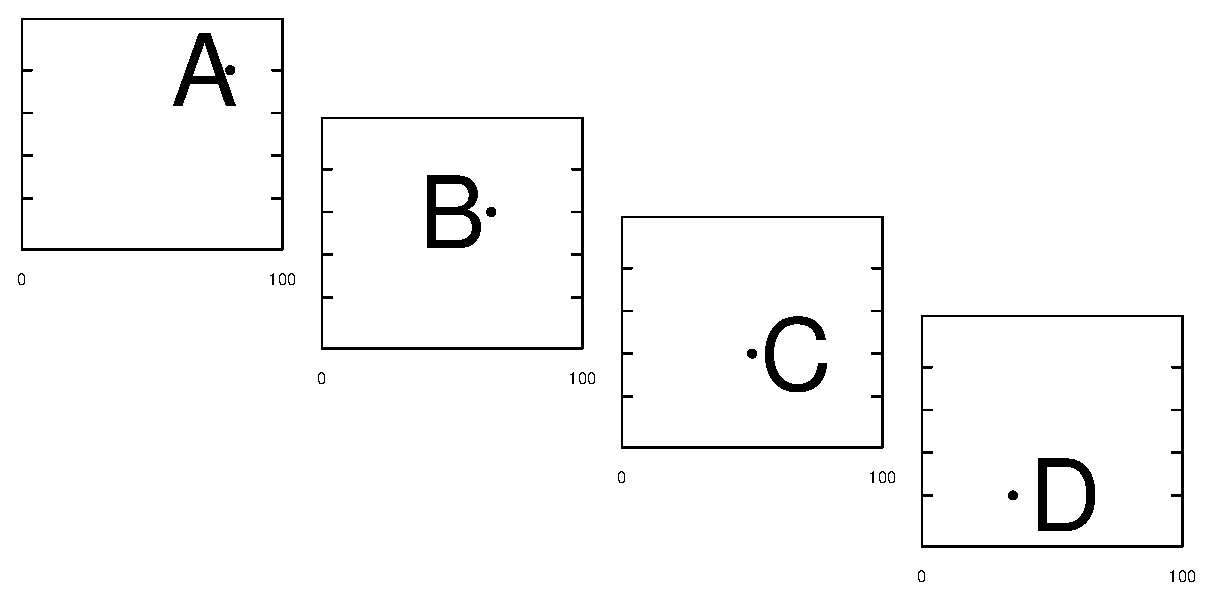
\includegraphics[width=0.53\textwidth]
   {Chapter21Graphs/Fig21_11bExperiments.eps}}  \hfill
   \subfloat[\textbf{Experiment to Understand Length Judgments. Suppose line A
is 100 units long. Assess the relative lengths of lines B, C and
D.}]{
\includegraphics[width=0.3\textwidth]
        {Chapter21Graphs/Fig21_11cExperiments.eps}}
 \subfloat[\textbf{Experiment to
Understand Angle Judgments. Suppose angle A is 100 units. Assess the
relative  values of angles B, C and D.}]{
   \includegraphics[width=0.45\textwidth]
   {Chapter21Graphs/Fig21_11dExperiments.eps}}  \hfill
   \subfloat[\textbf{Experiment to Understand
Area Judgments. Suppose circle A has area 100 units. Assess the
relative areas of circles B, C and D.}]{
\includegraphics[width=0.45\textwidth]
        {Chapter21Graphs/Fig21_11eExperiments.eps}}
    \caption{\label{F21:11aExperiments} \small Experiments in Judgments about Graphical Perception}
  \end{center}
\end{figure}



This chapter does not discuss the use of color because of the
complexities of coding and decoding it effectively. We refer
interested readers to Cleveland (1994, Section 3.13) and Tufte
(1990, Chapter 5) for further information.

The ordered list of graphical perception tasks can help the creator
choose the appropriate graphical form to portray a dataset. When
confronted with a choice of two graphical forms, a creator should
select the form that is least difficult for the viewer. Other things
being equal, a task that can be performed with little difficulty by
the viewer means that information can be transmitted more reliably.
To illustrate, we discuss two examples in which Table
\ref{T21:GraphPerception} can help you decide on the appropriate
graphical form for portraying a dataset.

\linejed

\textbf{Example \ref{S21:EmpiricalFoundations}.1: Distribution of
Premium Income}. The first example demonstrates some shortcomings of
the stacked bar chart. For this discussion, we return to Example
\ref{S21:DesignGuide}.1. Figure \ref{F21:DotPlotPremiumReceipts}(a)
is a three-dimensional stacked bar chart. We have already discussed
the substantial amount of chartjunk in this figure. Even without the
useless pseudo third dimension, the stacked bar chart requires the
viewer to make length judgments to understand, for example, the
distribution of annuity receipts over time. In contrast, the dot
plot in Figure \ref{F21:DotPlotPremiumReceipts}(b) requires the
viewer to make comparisons only according to positions along a
common scale. As described in Table \ref{T21:GraphPerception}, the
latter is an easier task, resulting in more reliable information for
the viewer. Thus, we conclude that the dot plot is preferred to the
stacked bar chart.

\linejed

\textbf{Example \ref{S21:EmpiricalFoundations}.2: Distribution of
Mortgages}. Our second example demonstrates the inadequacy of pie
charts. Figure \ref{F21:PieChartsMortgages} is an adaptation of the
figure on page 100 of the \emph{Life Insurance Fact Book} (1994). It
reports, for the years 1973, 1983 and 1993, commercial, 1- to
4-family, and farm mortgages as percentages of total mortgages. Pie
charts make comparisons difficult. For example, the graph makes it
difficult to detect whether farm mortgages are more prevalent than
1- to 4-family mortgages in 1983, or whether farm mortgage
percentages increased or decreased from 1973 to 1983. The comparison
of percentages across years is a linear operation, yet the pie
charts require us to decode angles, a difficult task according to
the ordering in Table \ref{T21:GraphPerception}. As with Example
\ref{S21:DesignGuide}.1, the charts in Figure
\ref{F21:PieChartsMortgages} make things worse by reporting in three
dimensions; these figures not only require us to decode volumes but
also add substantially to the chartjunk in the graphic. \emph{Only
nine numbers are reported in this graphic}, three years and two
percentages in each year. (The third percentage can be computed by
subtraction.)


\begin{figure}[htp]
  \begin{center}
    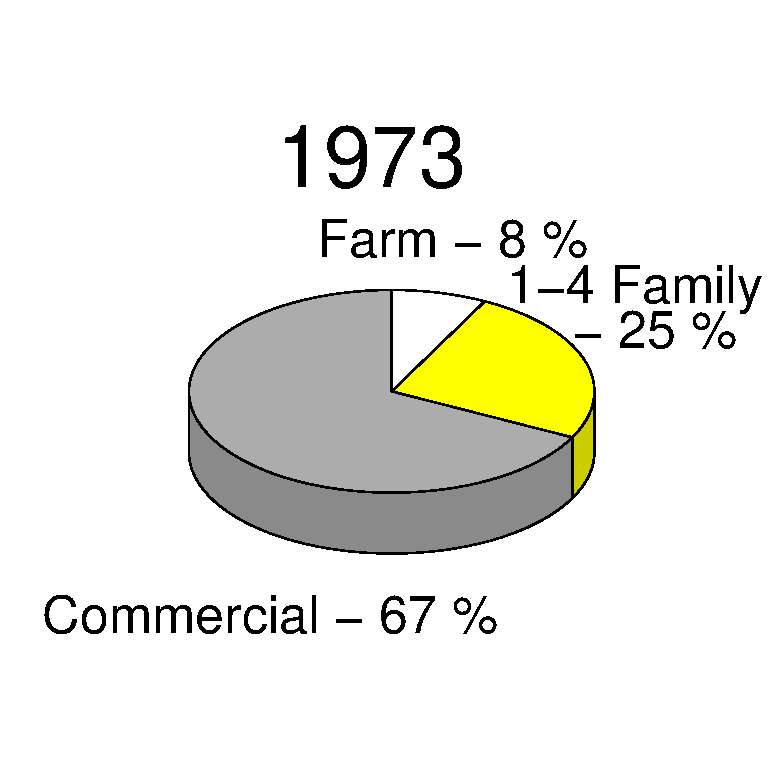
\includegraphics[width=0.31\textwidth]{Chapter21Graphs/F21Mortgage73.eps}
    \hfill
        \includegraphics[width=0.31\textwidth]{Chapter21Graphs/F21Mortgage83.eps} \hfill
            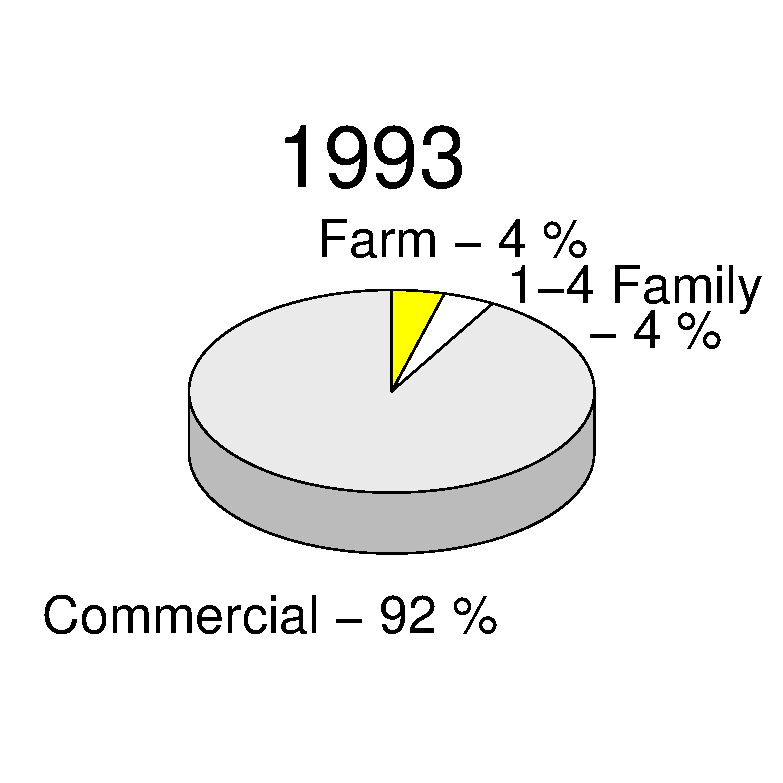
\includegraphics[width=0.31\textwidth]{Chapter21Graphs/F21Mortgage93.eps}
    \caption{\label{F21:PieChartsMortgages} \small Distribution of Mortgages for the Years 1973, 1983 and
1993. The three-dimensional pie chart is a poor graphical form for
making comparisons over time and across types of mortgages.}

  \end{center}
\end{figure}

If a graphic is needed, then the dot plot in Figure
\ref{F21:DotPlotPerCentMortgages} is more than sufficient. Here,
comparisons are made according to positions along a common scale, a
task easier than comparing angles. Pie charts require us to make
comparisons using angles, which are more difficult and less reliable
than comparisons using other graphical forms.

\begin{figure}[htp]
  \begin{center}
    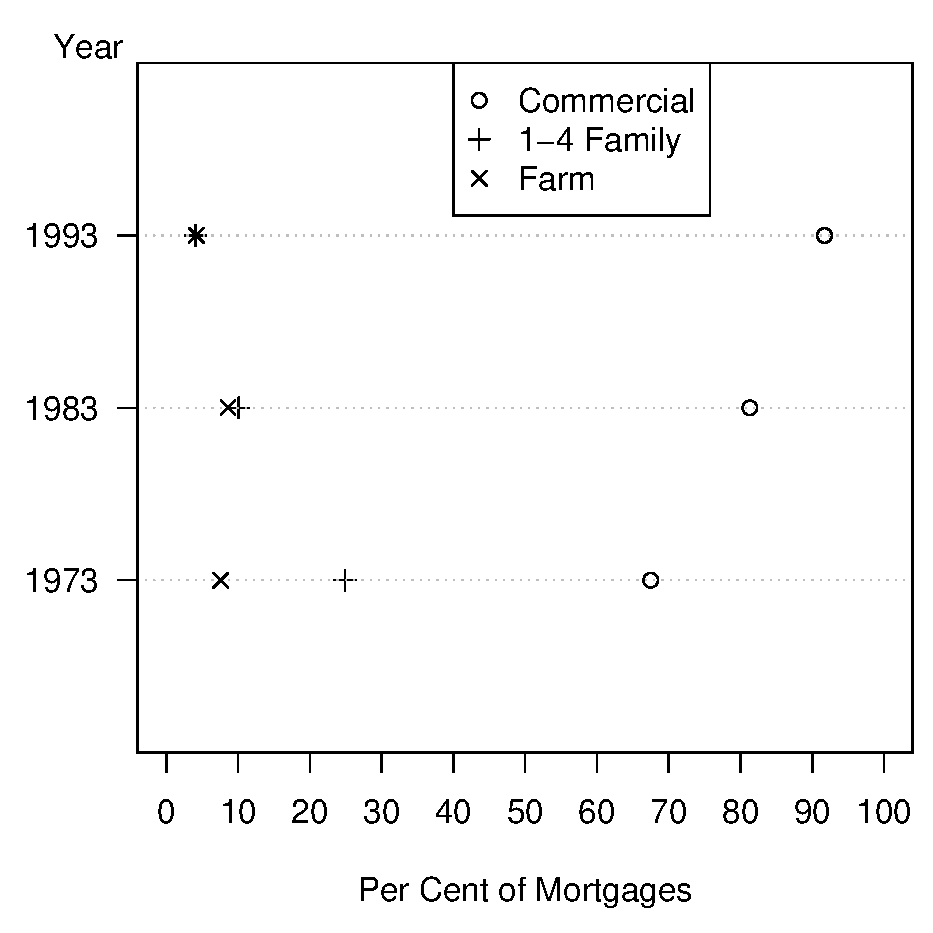
\includegraphics[width=0.5\textwidth]
        {Chapter21Graphs/Fig21_13DotPlotPerCentMortgages.eps}
    \caption{\label{F21:DotPlotPerCentMortgages} \small Commercial, 1- to 4-Family, and Farm Mortgages as
Percentages of Total Mortgages for 1973, 1983 and 1993. A negative
aspect of this graph is the overlap of the 1- to 4-family and farm
plotting symbols in 1983 and 1993.}
  \end{center}
\end{figure}

Although Figure \ref{F21:DotPlotPerCentMortgages} is a more
effective graph than Figure \ref{F21:PieChartsMortgages}, for these
data we recommend a tabular display (Table \ref{T21:Mortgages}),
which allows for clear comparisons across mortgage types and across
years. Further, more detailed information about mortgage percentages
is available in Table \ref{T21:Mortgages} than in Figure
\ref{F21:PieChartsMortgages} or \ref{F21:DotPlotPerCentMortgages}.
Of course, we can always superimpose the actual percentages, as is
often done with pie charts and as illustrated in Figure
\ref{F21:PieChartsMortgages}. Our response to this approach is to
question the worth of the entire graph. As with writing, each stroke
should offer new information; let creators of graphs make each
stroke tell!

\linejed

\subsection{Graphs as Units of Study}

Surveys of graphical practice in professional publications provide
an important database with which to assess prevalence of good and
bad practice and changes in practice over time. Tufte (1983, pp. 82-
86) discusses a survey of approximately 4,000 graphs randomly
selected from 15 news publications for the years 1974 to 1980. The
graphs were assessed for ``sophistication,'' defined as presentation
of relationship between variables, excluding time series or maps.
Cleveland and McGill (1985) report a similar survey of scientific
publications, assessing the prevalence of graphical errors.

\begin{table}[h] \scalefont{0.9}
\caption{\label{T21:Mortgages} Commercial, 1- to 4-Family, and Farm
Mortgages \newline as Percentages of Total Mortgages for 1973, 1983,
1993}
\begin{tabular}{lrrr}
\hline
 & \multicolumn{3}{c}{Year}\\
\hline Mortgage Type
 & 1973 & 1983 & 1993 \\ \hline
Commercial & 67.5 & 81.3 & 91.7 \\
1-4 Family & 24.9 & 10.1 & 4.1 \\
Farm & 7.6 & 8.6 & 4.2 \\ \hline
\end{tabular}
\scalefont{1.1111}
\end{table}

Harbert (1995) assessed every graph and table in the 1993 issues of
four psychology journals on 34 measures of quality. The measures of
quality were gleaned from the current research literature on graphic
quality. They were converted into a check sheet, and a check sheet
was filled out for each graph and table in the selected psychology
journals. Harbert's study yielded data on 439 graphs and tables. We
summarize the analysis of the 212 graphs.

Harbert assigned letter grades to the graphics: A, AB, B, BC, C, CD,
D, DF and F. These grades reflected her overall evaluation of the
graphs as communicators of statistical information. The grades were
converted to numerical values: 4.0, 3.5, 3.0, 2.5, 2.0, 1.5, 1.0,
0.5 and 0.0. The numerical values were the dependent variable in a
regression. The independent variables were the 34 measures of
quality, suitably coded. The purpose of the study was to determine
which factors were statistically significant predictors of the
grades assigned by an ``expert'' evaluator of graphics. By trial and
error, Harbert selected a multiple linear regression equation in
which all the predictors were statistically significant (5\% level)
and no other predictors achieved this level of significance when
added to the equation. Table \ref{T21:Factors} shows the variables
included in the regression equation ($R^2 = 0.612$).



\begin{table}[h] \scalefont{0.9}
\caption{\label{T21:Factors} Factors Affecting Assessment of Graphic
Quality, \newline ~Harbert Study}
\begin{tabular}{ll}
\hline
Variables with & Variables with\\
Positive Coefficients & Negative Coefficients \\ \hline Data-ink
ratio
& Proportion of page used by graphic\\
Comparisons made easy &Vertical labels on Y-axis \\
Sufficient data to make  &Abbreviations used \\
~~~a rich graphic&Optical art used \\
&Comparisons using areas or volumes \\
\hline
\end{tabular}
\scalefont{1.1111}
\end{table}



Data-ink ratio was defined by Tufte (1983, p. 93) as the
``proportion of the graphics ink devoted to the nonredundant display
of data-information'' or equivalently as ``1.0 minus the proportion
of a graphic that can be erased without loss of data-information.''
The data-ink ratio is more readily calculated than the data density
measure defined in Section \ref{S21:DesignGuide} of this paper.
Optical art is decoration that does not tell the viewer anything
new.

One variable that had been anticipated as very significant was data
density, which is difficult and time-consuming to measure. An
important finding of the study was that the easier-to-measure
data-ink ratio and proportion of page variables were sufficient to
predict the grades. A quotation from Harbert's thesis sums up the
finding: ``The highest grades were given to those graphics that take
up small proportions of the page, have a large data-ink ratio, make
comparisons easy, have enough data points, have horizontally printed
labels, do not have abbreviations, do not have optical art, and do
not use volume or 3-D comparisons'' (Harbert 1995, p. 56).

As a small follow-up study to Harbert's work, we examined each of
the 19 non-table graphics in the \emph{Life Insurance Fact Book}
(1994), assessing them on seven negative factors. Table
\ref{T21:GraphsFactors} shows the percentage of graphs that
displayed each of the negative factors.


\begin{table}[h] \scalefont{0.9}
\caption{\label{T21:GraphsFactors} Percentage of Graphs Displaying
Negative Factors \newline in Life Insurance Fact Book 1994}
\begin{tabular}{lc}
\hline
 Negative Factor &Percentage \\ &of Graphics \\ \hline Use of 3-D bars & ~~~79 \%
 \\
Grid lines too dense &79 \\
 Making comparison of time series values
hard &37\\
 Use of stacked bars & 37 \\
 Growth displayed poorly &32\\
 Use of
lines that are wider than need be& 16\\ Use of pies &5\\ \hline
\end{tabular}
\scalefont{1.1111}
\end{table}




Our review suggests that every graphic could have been reduced by
50\% to 75\% without loss of clarity. This observation is in keeping
with Harbert's finding about the proportion-of-page variable. In a
word, the graphs in the \emph{Life Insurance Fact Book} could be
produced much more ably. Doing so would improve the quality of
communication and would potentially increase the respect with which
knowledgeable professionals in other fields view the insurance
industry.

We hope that other investigators will engage in further study of
graphic practice in actuarial publications. By using data from such
studies, the profession can improve its practice, making
communications efficient and precise.

\section{Concluding Remarks}\label{S21:Conclude}

The Society of Actuaries' motto is a quotation of Ruskin: ``The work
of science is to substitute facts for appearances and demonstrations
for impressions.'' Armed with the guidelines outlined in this paper
and discussed further in the references, actuaries can be leaders in
presenting data graphically, thus substituting demonstrations for
impressions. Surveys of recent actuarial literature should be the
basis for assessing current practice. Editors and referees of
professional publications can be especially influential in bringing
about a rapid improvement in standards of practice. Moreover,
actuaries can recommend and use statistics textbooks that pay
attention to graphic quality.

Because actuaries read material that contains graphs, they are
consumers. They should become tough customers! All too often the
defaults in spreadsheet and statistical graphics software become the
norm. Actuaries should not allow the choices made by software
programmers to drive graphic quality or standards. Although it is
easy to create graphs using defaults in the graphics software, the
resulting graphs are seldom fully satisfactory. If a graph is not
worth doing well, let's leave it out of our publications.


\section{Further Reading and References}\label{S21:References}

In addition to the references listed, other resources are available
to actuaries interested in improving their graphic design skills.
Like the Society of Actuaries, another professional organization,
the American Statistical Association (ASA), has special interest
sections. In particular, the ASA now has a section on statistical
graphics. Interested actuaries can join ASA and that section to get
the newsletter \emph{Statistical Computing \& Graphics}. This
publication has examples of excellent graphical practice in the
context of scientific discovery and application.

The technical \emph{Journal of Computational and Graphical
Statistics} contains more in-depth information on effective graphs.
We also recommend accessing and using the \emph{ASA Style Guide }at
http:
//www.amstat.org/publications/style-guide.html as an aid to
effective communication of quantitative ideas.

\bigskip

\textbf{Chapter References}

\begin{multicols}{2}

\scalefont{0.9}

American Council of Life Insurance. Various years. \emph{Life
Insurance Fact Book}. Washington, D.C.: ACLI.

Cleveland, William S. (1994). \emph{The Elements of Graphing Data}.
Monterey, Calif.: Wadsworth.

Cleveland, William S. (1993).  \emph{Visualizing Data}. Summit,
N.J.: Hobart Press.

Cleveland, William S., Diaconis, P., and McGill. R. (1982).
Variables on scatterplots look more highly correlated when the
scales are increased. \emph{Science} 216, 1138-1141.

Cleveland, William S., and McGill, R. (1984). Graphical perception:
Theory, experimentation, and application to the development of
graphical methods. \emph{Journal of the American Statistical
Association} 79, 531-454.

Cleveland, William S., and McGill, R. (1985). Graphical perception
and graphical methods for analyzing and presenting scientific data.
\emph{Science} 229, 828-833.

Ehrenberg, A.S.C. (1977). Rudiments of Numeracy. \emph{Journal of
the Royal Statistical Society A} 140:277-97.

Frees, Edward W. (1996). \emph{Data Analysis Using Regression
Models.} Englewood Cliffs, N.J.: Prentice Hall.

Frees, Edward W. (1998). Relative Importance of Risk Sources in
Insurance Systems, \emph{North American Actuarial Journal} 2(2),
34-51.

Frees, Edward W., Kung, Yueh C., Rosenberg, Marjorie A., Young,
Virginia R., and Lai, Siu-Wai (1997). Forecasting Social Security
Assumptions, \emph{North American Actuarial Journal} 1(3), 49-82.

Harbert, D. (1995). The Quality of Graphics in 1993 Psychology
Journals, Senior honors thesis, University of Wisconsin-Madison.

Huff, D. (1954). \emph{How To Lie with Statistics}. New York:
Norton.

Schmid, C.F. (1992). \emph{Statistical Graphics: Design Principles
and Practices} Malabar, Fla.: Krieger Publishing Co.

Schmit, Joan T., and Roth, K. (1990). Cost Effectiveness of Risk
Management Practices, \emph{Journal of Risk and Insurance} 57,
455-470.

Strunk, W., and White, E.B. (1979). \emph{The Elements of Style}.
3rd ed. New York: Macmillan.

Tufte, Edward R. (1983). T\emph{he Visual Display of Quantitative
Information}. Cheshire, Conn.: Graphics Press.

Tufte, Edward R. (1990). \emph{Envisioning Information}. Cheshire,
Conn.: Graphics Press.

Tufte, Edward R. (1997). \emph{Visual Explanations}. Cheshire,
Conn.: Graphics Press.

Tukey, John (1977). \emph{Exploratory Data Analysis}. Reading,
Mass.: Addison-Wesley.

University of Chicago Press (1993). \emph{The Chicago Manual of
Style}. 14th ed. Chicago, Ill.

\scalefont{1.1111}

\end{multicols}


\end{document}

\input{Appendices/Preface03May2009.tex}
\input{Chapter1/Chap1Intro02May2009.tex}

\part{Linear Regression}
\input{Chapter2/Chap2_Basics02May2009.tex}
\input{Chapter3/Chap3MLR02May2009.tex}
\input{Chapter4/Chap4_ANOVA02May2009.tex}
\input{Chapter5/Chap5VarSelection02May2009.tex}
\input{Chapter6/Chap6Interpretation02May2009.tex}

\part{Topics in Time Series}
\setcounter{chapter}{6}
\chapter{Modeling Trends}
{\small \textit{Chapter Preview}. This chapter begins our study of
time series data by introducing techniques to account for major
patterns, or trends, in data that evolve over time. The focus is on
how regression techniques developed in earlier chapters can be used
to model trends. Further, new techniques, such differencing data,
allow us to naturally introduce a random walk, an important model of
efficient financial markets.}


\section{Introduction}

\subsubsection*{Time Series and Stochastic Processes}

Business firms are not defined by physical structures such as the
solid stone bank building that symbolizes financial security. Nor
are businesses defined by space alien invader toys that they
manufacture for children. Business firms are comprised of several
complex, interrelated processes. A \emph{process} is a series of
actions or operations that lead to a particular end.

Processes are not only the building blocks of businesses, they also
provide the foundations for our everyday lives. We may go to work or
school every day, practice martial arts or study statistics. These
are regular sequences of activities that define us. In this text,
our interest is in modeling \index{time series terms and
concepts!stochastic process} \emph{stochastic processes}, defined to
be ordered collections of random variables, that quantify a process
of interest.

\marginparjed{A time series is a single measurement of a process
that yields a variable over time, denoted by $y_1,...,y_T$.}

Some processes evolve over time, such as daily trips to work or
school and the quarterly earnings of a firm. We use the term
\emph{longitudinal data} for measurements of a process that evolves
over time.\index{time series terms and concepts!longitudinal data} A
single measurement of a process yields a variable over time, denoted
by $y_1,...,y_T,$ and referred to as a \emph{time series}.
\index{time series terms and concepts!time series}In this portion of
the text, we follow common practice and use $T$ to denote the number
of observations available (instead of $n$). Chapter 10 will describe
another type of longitudinal data where we examine a cross-section
of entities, such as firms, and examine their evolution over time.
This type of data is also known as \emph{panel data}.

Collections of random variables may be based on orderings other than time.
For example, hurricane claim damages are recorded at the place where the
damage has occurred and thus are ordered spatially. As another example,
evaluation of an oil-drilling project requires taking samples of the earth
at various longitudes, latitudes and depths. This yields observations
ordered by the three dimensions of space but not time. As yet another
example, the study of holes in the ozone layer requires taking atmospheric
measurements. Because the interest is in the trend of ozone depletion, the
measurements are taken at various longitudes, latitudes, heights and time.
Although we consider only processes ordered by time, in other studies of
longitudinal data you may see alternatives orderings. Data that are not
ordered are called \emph{cross-sectional}.

\marginparjed{Cross-sectional data are not ordered by time.}

\subsubsection*{Time Series versus Causal Models}\index{time series models!causal}

Regression methods can be used to summarize many time series data
sets. However, simply using regression techniques without
establishing an appropriate context can be disastrous. This concept
is reinforced by an example based on Granger and Newbold's (1974)
work.

\linejed

\textbf{Example: Spurious Regression.} Let $\{\varepsilon_{x,t}\}$ and $%
\{\varepsilon_{y,t}\}$\ be two independent sequences, each of which
also has a standard normal distribution. From these, recursively
construct the variables $x_t = 0.5 + x_{t-1} + \varepsilon_{x,t}$
and $y_t = 0.5 + y_{t-1} + \varepsilon_{y,t}$, using the initial
conditions $x_0=y_0=0$. (In Section 7.3, we will identify $x_t$\ and
$y_t$\ as random walk models.) Figure \ref{F7:SpurCorr} shows a
realization of \{$x_t$\} and \{$y_t$\}, generated for $T=50$
observations using simulation. The left-hand panel shows the growth
of each series over time - the increasing nature is due to the
addition of 0.5 at each time point. The right-hand panel shows a
strong relationship between \{$x_t$\} and \{$y_t$\} - the
correlation between these two series turns out to be 0.92. This is
despite the fact that the two series were generated
\emph{independently. }Their apparent relationship, said to be
\emph{spurious}, is because both are related to the growth over
time.


\begin{figure}[htp]
  \begin{center}
    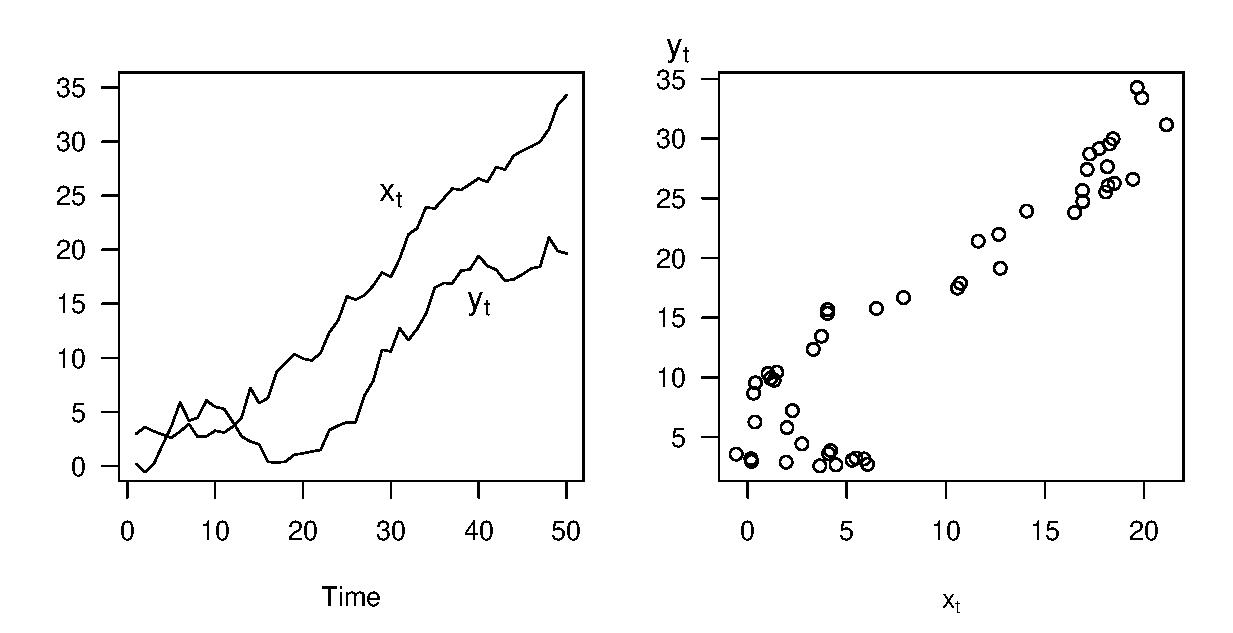
\includegraphics[width=1\textwidth]{Chapter7Trend/Figure71SpurCorr.eps}
    \caption{\label{F7:SpurCorr} \small Spurious
Regressions. The left-hand panel shows two time series that are
increasing over time. The right-hand panel shows a scatter plot of
the two series, suggesting a positive relationship between the two.
The relationship is spurious in the sense that both series are
driven by growth over time, not their positive dependence on one
another.}
  \end{center}
\end{figure}

\linejed

In a longitudinal context, regression models of the form%
\begin{equation*}
y_t = \beta_0 + \beta_1 x_t + \varepsilon_t
\end{equation*}
are known as \emph{causal models}. Causal models are regularly
employed in econometrics, where it is assumed that economic theory
provides the information needed to specify the causal relationship
($x$ ``causes'' $y$). In contrast, statistical models can only
validate empirical relationships (``correlation, not causation'').
In the spurious regression example, both variables evolve over time
and so a model of how one variable influences another needs to
account for time patterns of both the left- and right-hand side
variables. Specifying causal models for actuarial applications can
be difficult for this reason - time series patterns in the
explanatory variables may mask or induce a significant relationship
with the dependent variable. In contrast, regression modeling can be
readily applied when explanatory variables are simply functions of
time, the topic of the next section. This is because functions of
time are deterministic and so will not exhibit time series patterns.

\marginparjed{Regression models can be readily applied when
explanatory variables are functions of time.}

Causal models also suffer from the drawback that their applications
are limited for forecasting purposes. This is because in order to
make a forecast of a future realization of the series, for example
$y_{T+2}$, one needs to have knowledge (or a good forecast) of
$x_{T+2},$ the value of the explanatory variable at time $T+2$. If
$x$ is a known function of time (as in the next section), then this
is not an issue. Another possibility is to use a lagged value of $x$
such as $y_t = \beta_0 + \beta_1 x_{t-1} + \varepsilon_t,$ so that
one-step predictors are possible (we can use the equation to predict
$y_{T+1}$ because $x_T$ is known at time $T$).

\section{Fitting Trends in Time}\label{S7:Trends}

\subsubsection*{Understanding Patterns over Time}

\marginparjed{A forecast is a prediction of a future value of a time
series.}

\emph{Forecasting} is about predicting future realizations of a time
series. Over the years, analysts have found it convenient to
decompose a series into three types of patterns: trends in time
($T_t$), seasonal ($S_t$), and random, or irregular, patterns
($\varepsilon_t$). A series can then be forecast by extrapolating
each of the three patterns. The trend is that part of a series that
corresponds to a long-term, slow evolution of the series. This is
the most important part for long-range forecasts. The seasonal part
of the series corresponds to aspects that repeat itself
periodically, say over a year. The irregular patterns of a series
are short-term movements that are typically harder to
anticipate.\index{time series terms and concepts!forecast}

Analysts typically combine these patterns in two ways: in an
additive fashion,
\begin{equation}\label{E7:1}
y_t = T_t + S_t + \varepsilon_t,
\end{equation}
or in a multiplicative fashion,
\begin{equation}\label{E7:2}
y_t = T_t \times S_t + \varepsilon_t.
\end{equation}
Models without seasonal components can be readily handled by using
$S_t=0$ for the additive model in equation (\ref{E7:1}) and $S_t=1$
for the multiplicative model in equation (\ref{E7:2}). If the model
is purely multiplicative such that $y_t = T_t \times S_t \times
\varepsilon_t$, then it can be converted to an additive model by
taking logarithms of both sides.

\marginparjed{A plot of $y_t$ versus $t$ is called a time series
plot.}

\index{plots!time series}

It is instructive to see how these three components can be combined
to form a series of interest. Consider the three components in
Figure \ref{F7:LinearTrend}. Under the additive model, the trend,
seasonal and random variation components are combined to form the
series that appears in the lower right-hand panel. A plot of $y_t$
versus $t$ is called a \emph{time series plot}. In time series
plots, the convention is to connect adjacent points using a line to
help us detect patterns over time.

When analyzing data, the graph in the lower right-hand panel is the
first type of plot that we will examine. The goal of the analysis is
to go backwards - that is, we wish to decompose the series into the
three components. Each component can then be forecast which will
provide us with forecasts that are reasonable and easy to interpret.


\begin{figure}[htp]
  \begin{center}
    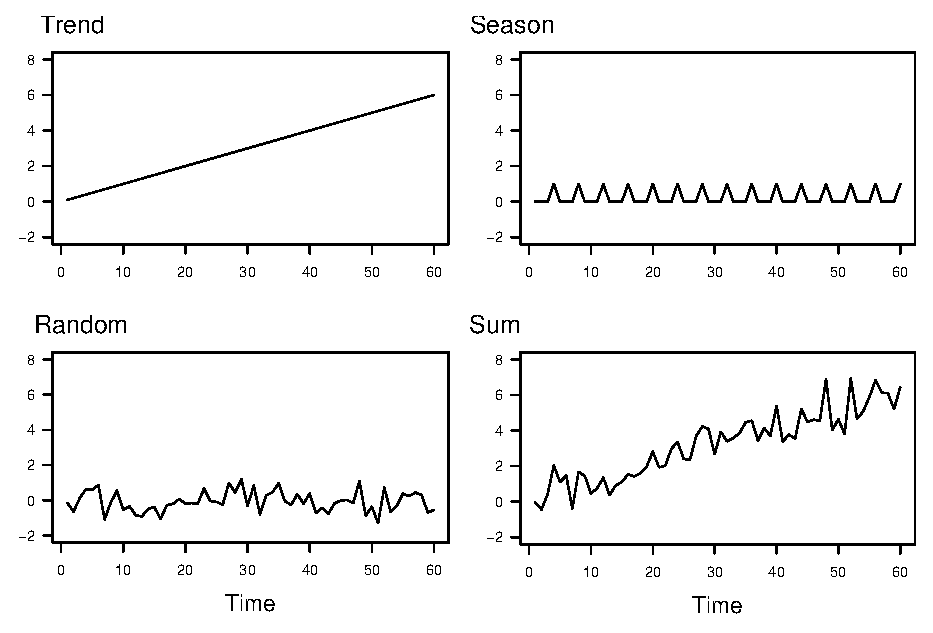
\includegraphics[width=1\textwidth]{Chapter7Trend/Components.eps}
    \caption{\label{F7:LinearTrend} \small Time Series
Plots of Response Components. The linear trend component appears in
the upper left-hand panel, the seasonal trend in the upper right and
the random variation in the lower left. The sum of the three
components appears in the lower right-hand panel.}
  \end{center}
\end{figure}


\subsubsection*{Fitting Trends in Time}

The simplest type of time trend is a complete lack of trend.
Assuming that the observations are identically and independently
distributed (\emph{i.i.d.}), then we could use the model
\begin{equation*}
y_t = \beta_0 + \varepsilon_t.
\end{equation*}
For example, if you are observing a game of chance such as bets
placed on the roll of two dice, then we typically model this as an
i.i.d. series.

\marginparjed{The linear trend in time model is a regression model
with a straight line in time as the regression function.}

Fitting polynomial functions of time is another type of trend that
is easy to interpret and to fit to the data. We begin with a
straight line for our polynomial function of time, yielding the
\emph{linear trend in time model},\index{time series models!linear
trend in time}
\begin{equation}\label{E7:3}
y_t = \beta_0 + \beta_1 t + \varepsilon_t.
\end{equation}
Similarly, regression techniques can be used to fit other functions
that represent trends in time. Equation (\ref{E7:3}) is easily
extended to handle a \emph{quadratic trend in time},\index{time
series models!quadratic trend in time}
\begin{equation*}
y_t = \beta_0 + \beta_1 t + \beta_2 t^2 + \varepsilon_t,
\end{equation*}
or a higher-order polynomial.

\linejed

\empexjed{HKExchange}\index{datasets!Hong Kong exchange rates}

\textbf{Example: Hong Kong Exchange Rates.}\ecaptionjed{Hong Kong
Exchange Rates} For travelers and firms, exchange rates are an
important part of the monetary economy. The exchange rate that we
consider is the number of Hong Kong dollars that one can purchase
for one US dollar. We have $T=502$ daily observations for the period
April 1, 2005 through May 31, 2007 that were obtained from the
Federal Reserve (H10 report). Figure \ref{F7:HKFits} provides a time
series plot of the Hong Kong exchange rate.

\begin{figure}[htp]
  \begin{center}
        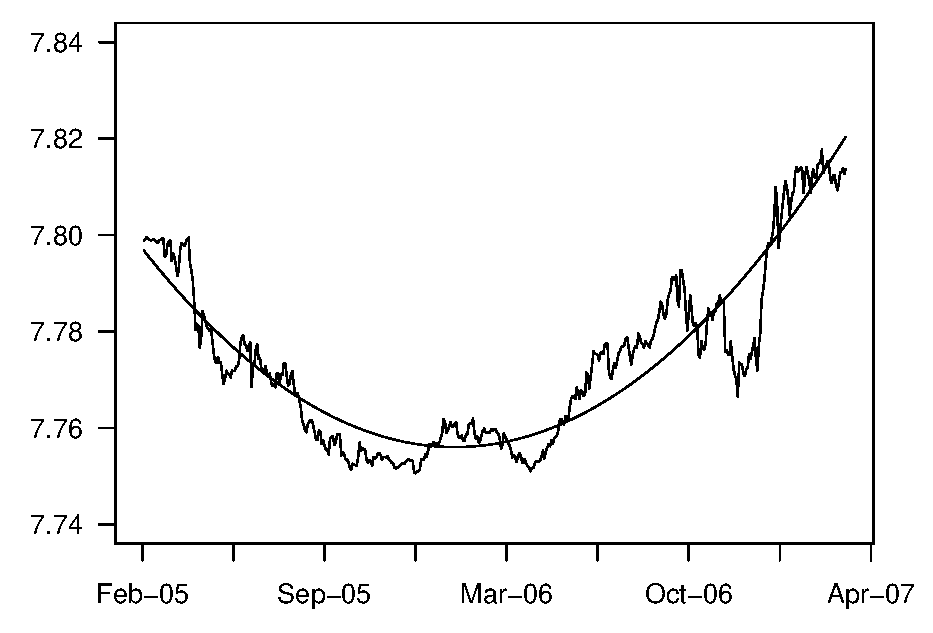
\includegraphics[width=.6\textwidth]{Chapter7Trend/HKFits.eps}
    \caption{\label{F7:HKFits} \small Time Series Plot of Hong Kong
    Exchange Rates with Fitted Values Superimposed. The fitted values are from a regression using a quadratic time trend.
     \emph{Source}: Foreign Exchange Rates (Federal Reserve, H10 report).}
  \end{center}
\end{figure}


Figure \ref{F7:HKFits} shows a clear quadratic trend in the data. To
handle this trend, we use $t=1,...,502$, as an explanatory variable
to indicate the time period. The fitted regression equation turns
out to be:
\begin{equation*}
\begin{tabular}{cccc}
$\widehat{INDEX}_t = $ & $7.797$ & $-3.68\times 10^{-4}t$ &
$+8.269\times
10^{-7}t^2$ \\
{\small $t$-statistics} & {\small (8,531.9)} & {\small (-44.0)} &
{\small (51.2)}
\end{tabular}
.
\end{equation*}
The coefficient of determination is a healthy $R^2=92.9\%$ and the
standard deviation estimate has dropped from $s_{y}=0.0183$ down to
$s=0.0068$ (our residual standard deviation). Figure \ref{F7:HKFits}
shows the relationship between the data and fitted values through
the time series plot of the exchange rate with the fitted values
superimposed. To apply these regression results to the forecasting
problem, suppose that we wanted to predict the exchange rate for
April 1, 2007, or $t=503$. Our prediction is
\begin{equation*}
\widehat{INDEX}_{503} = 7.797 - 3.68 \times 10^{-4}(503) + 8.269
\times 10^{-7}(503)^2 = 7.8208.
\end{equation*}

The overall conclusion is that the regression model using a
quadratic term in time $t$ as an explanatory variable fits the data
well. A close inspection of Figure \ref{F7:HKFits}, however, reveals
that there are patterns in the residuals where the responses are in
some places consistently higher and in other places consistently
lower than the fitted values. These patterns suggest that we can
improve upon the model specification. One way would be to introduce
a higher order polynomial model in time. In Section 7.3, we will
argue that the random walk is an even better model for this data.

\linejed

Other nonlinear functions of time may also be useful. To illustrate,
we might study some measure of interest rates over time ($y_t$) and
be interested in the effect of a change in the economy (such as the
advent of a war). Define $z_t$ to be a binary variable that is zero
before the change occurs and is one during and after the change.
Consider the model,
\begin{equation} \label{E7:4}
y_t = \beta_0 + \beta_1 z_t + \varepsilon_t.
\end{equation}
Thus, using
\begin{equation*}
\mathrm{E~}y_t = \left\{
\begin{array}{ll}
\beta_0 + \beta_1 & if~z_t=1 \\
\beta_0 & if~z_t = 0
\end{array}
\right. ,
\end{equation*}
the parameter $\beta_1$ captures the expected change in interest
rates due to the change in the economy. See Figure
\ref{F7:RegimeSwitch}.


\begin{figure}[htp]
  \begin{center}
    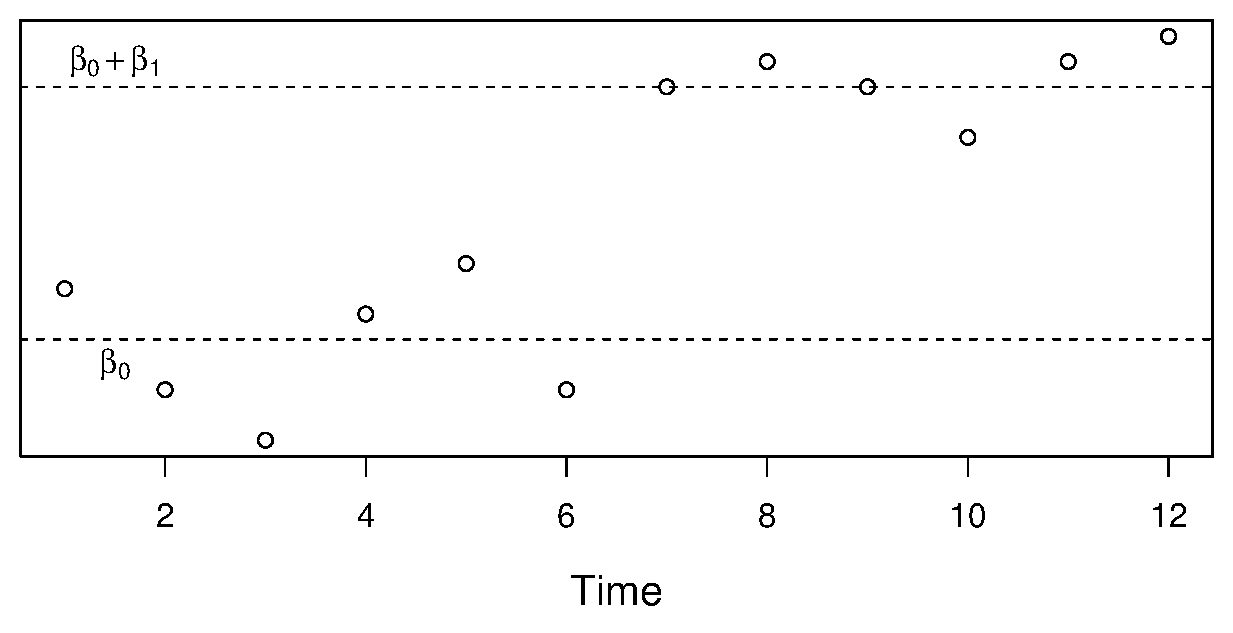
\includegraphics[width=0.6\textwidth]{Chapter7Trend/RegimeSwitch.eps}
    \caption{\label{F7:RegimeSwitch} \small Time
Series Plot of Interest Rates. There is a clear shift in the rates
due to a change in the economy. This shift can be measured using a
regression model with an explanatory variable to indicate the
change.}
  \end{center}
\end{figure}

\linejed

\index{examples!long-term stock returns}

\textbf{Example: Regime-Switching Models of Long-Term Stock
Returns.}\ecaptionjed{Long-Term Stock Returns} With the assumption
of normality, we can write the model in equation (\ref{E7:4}) as
\begin{equation*}
y_t \sim \left\{
\begin{array}{ll}
N(\mu_1, \sigma^2) & t < t_0 \\
N(\mu_2, \sigma^2)& t \geq t_0
\end{array}
\right. ,
\end{equation*}
where $\mu_1 = \beta_0$, $\mu_2 = \beta_0 + \beta_1$ and $t_0$ is
the change point. A \emph{regime-switching} model generalizes this
concept, primarily by assuming that the change point is not known.
Instead, one assumes there exists a transition mechanism that allows
us to shift from one ``regime'' to another with a probability that
is typically estimated from the data. In this model, there is a
finite number of states, or ``regimes.'' Within each regime, a
probabilistic model is specified, such as the (conditionally)
independent normal distribution ($N(\mu_2, \sigma^2)$). One could
also specify an autoregressive or conditionally autoregressive model
that we will define in Chapter 8. Further, there is a conditional
probability of transiting from one state to another (so-called
``Markov'' transition probabilities).

Hardy (2001) introduced regime-switching models to the actuarial
literature where the dependent variable of interest was the
long-term stock market return as measured by  monthly returns on (1)
the Standard and Poor's 500 and the Toronto Stock Exchange 300.
Hardy considered two and three regime models for data over 1956 to
1999, inclusive. Hardy showed how to use the parameter estimates
from the regime-switching model to compute option prices and risk
measures for equity-linked insurance contracts.

\linejed


\subsubsection*{Fitting Seasonal Trends}

Regular periodic behavior is often found in business and economic
data. Because such periodicity is often tied to the climate, these
trends are called \emph{seasonal components}. Seasonal trends can be
modeled using the same techniques as with regular, or aperiodic,
trends. The following example shows how to capture periodic behavior
using seasonal binary variables.\index{time series terms and
concepts!seasonal component}

\linejed

\textbf{Example: Trends in Voting.}\ecaptionjed{Voting Trends} On
any given election day, the number of voters that actually turn out
to voting booths depend on a number of factors: the publicity that
an election race has received, the issues that are debated as part
of the race, other issues facing voters on election day, and
nonpolitical factors, such as the weather. Now, potential political
candidates base their projections of campaign financing, and chances
of winning an election, on forecasts of the number of voters who
will actually participate in an election. Decisions as to whether or
not to participate as a candidate must be made well in advance;
generally, so far in advance that well-known factors such as the
weather on election day can not be used in generating forecasts.

We consider here the number of Wisconsin voters who participated in
statewide elections over the period 1920 through 1990. Although the interest
is in forecasting the actual number of voters, we consider voters as a
percentage of the qualified voting public. Dividing by the qualified voting
public controls for the size of the population of voters; this enhances
comparability between the early and latter parts of the series. Because
mortality trends are relatively stable, reliable projections of the
qualified voting public can be readily attained. Forecasts of the percentage
may then be multiplied by projections of the voting public to obtain
forecasts of the actual voter turnout.

To specify a model, we examine Figure \ref{F7:WiscVotes}, a time
series plot of the voter turnout as a percent of the qualified
voting public. This figure displays the low voter turnout in the
early part of the series, followed by larger turnout in the 1950's
and 1960's, followed by a smaller turnout in the 1980's. This
pattern can be modeled using, for example, a quadratic trend in
time. The figure also displays a much larger turnout in presidential
elections years. This periodic, or seasonal, component can be
modeled using a binary variable. A candidate model is
\begin{equation*}
y_t=\beta_0+\beta_1t+\beta_2t^2+\beta_{3}z_t+\varepsilon _t,
\end{equation*}
where

\begin{equation*}
z_t=\left\{
\begin{array}{ll}
1 & if~\mathrm{presidential\ election\ year} \\
0 & otherwise
\end{array}
\right. .
\end{equation*}
Here, $\beta_{3}z_t$ captures the seasonal component in this model.

Regression was used to fit the model. The fitted model provided a
good fit of the data - the coefficient of determination from the fit
was $R^2=89.6\%.$ Figure \ref{F7:WiscVotes} shows a strong
relationship between the fitted and actual values.

\begin{figure}[htp]
  \begin{center}
    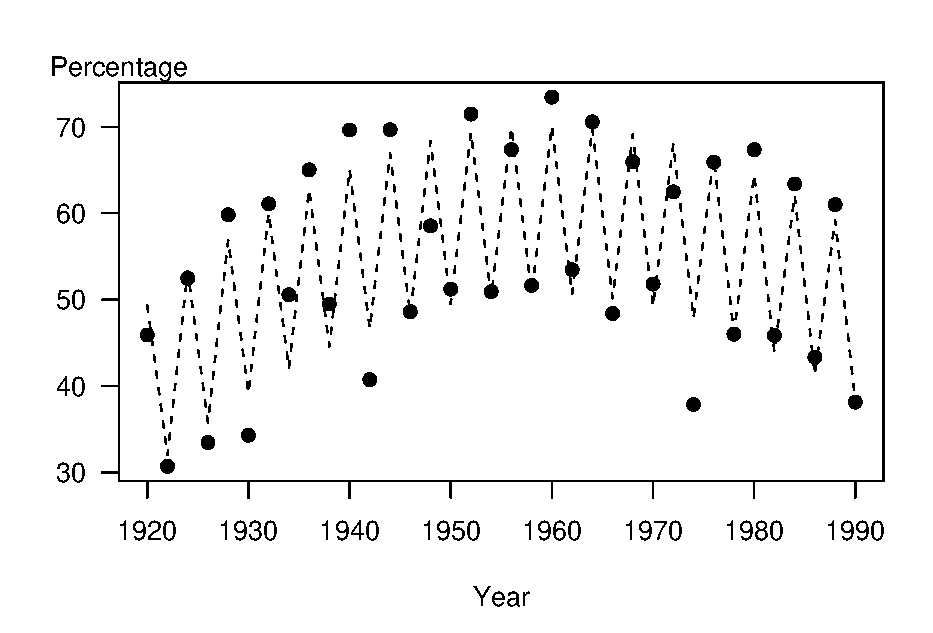
\includegraphics[height=2.5in, width=4.5in]{Chapter7Trend/WiscVotes.eps}
    \caption{\label{F7:WiscVotes} \small Wisconsin
Voters as a Percentage of the Qualified Voting Public, by Year. The
opaque circles represent the actual voting percentages. The dashed
lines represent the fitted trend, using a quadratic trend in time
plus a binary variable to indicate a presidential election year.}
  \end{center}
\end{figure}

\linejed

The voting trend example demonstrates the use of binary variables to
capture seasonal components. Similarly, seasonal effects may be also
be represented using categorical variables, such as
\begin{equation*}
z_t=\left\{
\begin{array}{ll}
1 & if\text{~spring} \\
2 & if\text{~summer} \\
3 & if\text{~fall} \\
4 & if\text{~winter}%
\end{array}%
\right. .
\end{equation*}

Another way of capturing seasonal effects is through the use of
trigonometric functions. Further discussion of the use of trigonometric
functions to handle seasonal components is in Section 9.3.

\marginparjed{Removal of seasonal patterns is known as seasonal
adjustment.}\index{time series terms and concepts!seasonal
adjustment}

Removal of seasonal patterns is known as \emph{seasonal adjustment}.
This strategy is appropriate in public policy situations where
interest centers on interpreting the resulting ``seasonally adjusted
series.'' For example, government agencies typically report
industrial manufacturing revenues in terms of seasonally adjusted
numbers, with the understanding that known holiday and weather
related patterns are accounted for when reporting growth. However,
for most actuarial and risk management applications, the interest is
typically in forecasting the variation of the entire series, not
just the seasonally adjusted portion.

\subsubsection*{Reliability of Time Series Forecasts}

Time series forecasts are sometimes called ``naive'' forecasts. The
adjective ``naive'' is somewhat ironic because many time series
forecasting techniques are technical in nature and complex to
compute. However, these forecasts are based on extrapolating a
single series of observations. Thus, they are naive in the sense
that the forecasts ignore other sources of information that may be
available to the forecaster and users of the forecasts. Despite
ignoring this possibly important information, time series forecasts
are useful in that they provide an objective benchmark that other
forecasts and expert opinions can be compared against.

\marginparjed{Projections should provide a user with a sense of the
reliability of the forecast.}

Projections should provide a user with a sense of the reliability of
the forecast. One way of quantifying this is to provide forecasts
under ``low-intermediate-high'' sets of assumptions. For example, if
we are forecasting the national debt, we might do so under three
scenarios of the future performance of the economy. Alternatively,
we can calculate prediction intervals using many of the models for
forecasting that are discussed in this text. Prediction intervals
provide a measure of reliability that can be interpreted in a
familiar probabilistic sense. Further, by varying the desired level
of confidence, the prediction intervals vary, thus allowing us to
respond to ``what if'' types of questions.

For example, in Figure 21.10 you will find a comparison of
``low-intermediate-high'' projections to prediction intervals for
forecasts of the inflation rate (CPI) used in projecting Social
Security funds. The low-intermediate-high projections are based on a
range of expert opinions and thus reflect variability of the
forecasters. The prediction intervals reflect innovation uncertainty
in the model (assuming that the model is correct). Both ranges give
the user a sense of reliability of the forecasts although in
different ways.

Prediction intervals have the additional advantage in that they
quantify the fact that forecasts become less reliable the further
that we forecast into the future. Even with cross-sectional data, we
saw that the farther away we were from the main part of the data,
the less confident we felt in our predictions. This is also true in
forecasting for longitudinal data. It is important to communicate
this to consumers of forecasts, and prediction intervals are a
convenient way of doing so.

\marginparjed{In forecasting, the primary concern is for the most
recent part of the series.}

In summary, regression analysis using various functions of time as
explanatory variables is a simple yet powerful tool for forecasting
longitudinal data. It does, however, have drawbacks. Because we are
fitting a curve to the entire data set, there is no guarantee that
the fit for the most recent part of the data will be adequate. That
is, for forecasting, the primary concern is for the most recent part
of the series. We know that regression analysis estimates give the
most weight to observations with unusually large explanatory
variables. To illustrate, using a linear trend in time model, this
means giving the most weight to observations at the end and \emph{at
the beginning }of the series. Using a model that gives large weight
to observations at the beginning of the series is viewed with
suspicion by forecasters. This drawback of regression analysis
motivates us to introduce additional forecasting tools. (Section 9.1
develops this point further.)

\section{Stationarity and Random Walk Models}\label{S7:RandomWalk}

A basic concern with processes that evolve over time is the
\emph{stability} of the process. For example: ``Is it taking me
longer to get to work since they put in the new stop light?'' ``Have
quarterly earnings improved since the new CEO took over?'' We
measure processes to improve or manage their performance and to
forecast the future of the process. Because stability is a
fundamental concern, we will work with a special kind of stability
called \emph{stationarity}.\bigskip

\boxedjed

\textbf{Definition.} \ Stationarity is the formal mathematical
concept corresponding to the ``stability'' of a time series of data.
A series is said to be (weakly) stationary if\index{time series
terms and concepts!stationary}

\begin{itemize}
\item the mean $\mathrm{E~}y_t$ does not depend on $t$ and

\item the covariance between $y_{s}$ and $y_t$ depends only on the
difference between time units, $|t-s|.$
\end{itemize}

\end{boxedminipage}

\bigskip

Thus, for example, under weak stationarity $\mathrm{E~}y_{4}=\mathrm{E~}%
y_{8} $ because the means do not depend on time and thus are equal. Further,
$\mathrm{Cov}(y_{4},y_{6})=\mathrm{Cov}(y_{6},y_{8})$, because $y_{4}$ and $%
y_{6}$ are two time units apart, as are $y_{6}$ and $y_{8}$. As
another implication of the second condition, note that $\sigma^2 =
\mathrm{Cov}(y_t, y_t) = \mathrm{Cov}(y_s, y_s) = \sigma^2$. Thus, a
weakly stationary series has a constant mean as well as a constant
variance (homoscedastic). Another type of stationarity known as
\emph{strict, or strong, stationarity} requires that the entire
distribution of $y_t$ be constant over time, not just the mean and
the variance.\index{time series terms and concepts!stationary!weak
stationarity}\index{time series terms and concepts!stationary!strong
stationarity}

\marginparjed{A weakly stationary series has a constant mean as well
as a constant variance (homoscedastic).}\index{homoscedasticity}


\subsubsection*{White Noise}

The link between longitudinal and cross-sectional models can be
established through the notion of a \emph{white noise }process. A
white noise process is a stationary process that displays no
apparent patterns through time. More formally, a white noise process
is simply a series that is \emph{i.i.d.}, identically and
independently distributed. A white noise process is only one type of
stationary process - Chapter 8 will introduce another type, an
autoregressive model.\index{time series models!white noise}


\marginparjed{A white noise process is a stationary process that
displays no apparent patterns through time - it is i.i.d.}

A special feature of the white noise process is that forecasts do
not depend on how far into the future that we wish to forecast.
Suppose that a series of observations, $y_1,...,y_T$, has been
identified as a white noise process. Let $\overline{y}$\ and $s_y$
denote the sample average and standard deviation, respectively. A
forecast of an observation in the future, say $y_{T+l}$, for $l$
lead time units in the future, is $\overline{y}$. Further, a
forecast interval is
\begin{equation}\label{E7:ForecastInterval}
\overline{y}\pm \ t_{T-1,1-\alpha/2} ~ s_y \sqrt{1+\frac{1}{T}}.
\end{equation}
In time series applications, because the sample size $T$ is
typically relatively large, we use the approximate 95\% prediction
interval $ \overline{y} \pm 2 s_y. $ This approximate forecast
interval ignores the parameter uncertainty in using $\overline{y}$\
and $s_y$\ to estimate the mean $\mathrm{E}~y$\ and standard
deviation $\sigma $\ of the series. Instead, it emphasizes the
uncertainty in future realizations of the series (known as
\emph{innovation uncertainty}). Note that this interval does
\emph{not} depend on the choice of $l$, the number of lead units
that we forecast into the future.\index{time series terms and
concepts!innovation uncertainty}


\marginparjed{The white noise model is both the least and the most
important of time series models.}

The white noise model is both the least and the most important of
time series models. It is the least important in the sense that the
model assumes that the observations are unrelated to one another, an
unlikely event for most series of interest. It is the most important
because our modeling efforts are directed towards reducing a series
to a white noise process. In time series analysis, the procedure for
reducing a series to a white noise process is called a
\emph{filter}. After all patterns have been filtered from the data,
the uncertainty is said to be \emph{irreducible}.\index{time series
terms and concepts!filter}\index{time series terms and
concepts!irreducible}

\subsubsection*{Random Walk}

We now introduce the \emph{random walk model}. For this time series
model, we will show how to filter the data simply by taking
differences.\index{time series models!random walk}

To illustrate, suppose that you play a simple game based on the roll
of the two dice. To play the game, you must pay \$7 each time you
roll the dice. You receive the number of dollars corresponding the
sum of the two dice, $c_t^{\ast}$. Let $c_t$ denote your winnings on
each roll, so that $c_t = c_t^{\ast} - 7$. Assuming that the rolls
are independent and come from the same distribution, the series
$\{c_t\}$ is a white noise process.

Assume that you start with initial capital of $y_0 = \$100$. Let
$y_t$ denote the sum of capital after the $t$th roll. Note that
$y_t$ is determined recursively by $y_t = y_{t-1} + c_t$. For
example, because you won \$3 on the first roll, $t=1$, you now have
capital $y_1 = y_0 + c_1$, or 103 = 100 + 3. Table \ref{T7:Winnings}
shows the results for the first five throws. Figure \ref{F7:RWDice}
is a time series plot of the sums, $y_t$, for the fifty throws.

\scalefont{0.9}
\begin{table}[h]
\caption{\label{T7:Winnings} Winnings for Five of the 50 Rolls}
\begin{center}
\begin{tabular}{c|ccccc}
\hline
$t$ & 1 & 2 & 3 & 4 & 5 \\
$c_t^{\ast }$ & 10 & 9 & 7 & 5 & 7 \\
$c_t$ & 3 & 2 & 0 & -2 & 0 \\
$~~y_t~~$ & ~103~ & ~105~ & ~105~ & ~103~ & 103 \\ \hline
\end{tabular}\end{center}\end{table}
\scalefont{1.1111}


\begin{figure}[htp]
  \begin{center}
    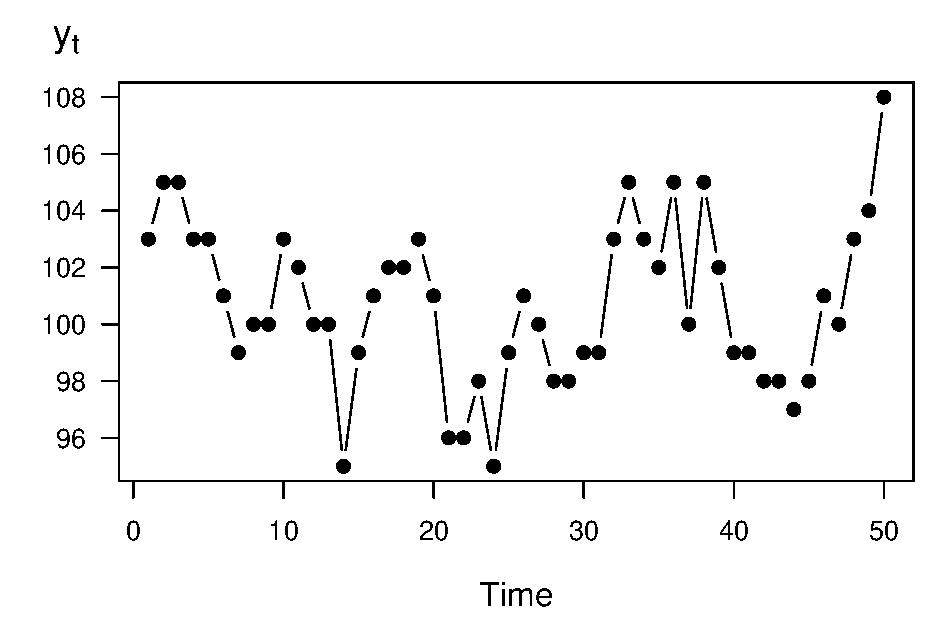
\includegraphics[width=.8\textwidth]{Chapter7Trend/RWDice.eps}
   \caption{\label{F7:RWDice} \small Time Series Plot of the Sum of Capital.}
  \end{center}
\end{figure}


The partial sums of a white noise process define a random walk
model. For example, the series $\{y_1, \ldots ,y_{50}\}$ in Figure
\ref{F7:RWDice} is a realization of the random walk model. The
phrase \emph{partial sum}\ is used because each observation, $y_t$,
was created by summing the winnings up to time $t$. For this
example, winnings, $c_t$, are a white noise process because the
amount returned, $c_t^{\ast}$, is i.i.d. In our example, your
winnings from each roll of the dice is represented using a white
noise process. Whether you win on one roll of the dice has no
influence on the outcome of the next, or previous, roll of the dice.
In contrast, your amount of capital at any roll of the dice is
highly related to the amount of capital after the next roll, or
previous roll. Your amount of capital after each roll of the dice is
represented by a random walk model.

\section{Inference using Random Walk Models}

The random walk is a commonly used time series model. To see how it
can be applied, we first discuss a few model properties. These
properties are then used to forecast and identify a series as a
random walk. Finally, this section compares the random walk to a
competitor, the linear trend in time model.

\subsubsection*{Model Properties}

To state the properties of the random walk, we first recap some
definitions. Let $c_1,\ldots ,c_T$ be $T$ observations from a white
noise process. A random walk can be expressed recursively as
\begin{equation} \label{E7:5}
y_t = y_{t-1} + c_t.
\end{equation}
By repeated substitution, we have
\begin{equation*}
y_t = c_t + y_{t-1} = c_t + \left( c_{t-1} + y_{t-2}\right) = \ldots
\end{equation*}
If we use $y_0$ to be the initial level, then we can express the
random
walk as%
\begin{equation}\label{E7:6}
y_t = y_0 + c_1 + \ldots + c_t.
\end{equation}
Equation (\ref{E7:6}) shows that a random walk is the partial sum of
a white noise process.

\marginparjed{A random walk is the partial sum of a white noise
process.}

The random walk is \emph{not} a stationary process because the
variability, and possibly the mean, depends on the time point at
which the series is observed. Taking the expectation and variance of
equation (\ref{E7:6}) yields the mean level and variability of the
random walk process:
\begin{equation*}
\mathrm{E~}y_t = y_0 + t\mu_c\text{ \ \ and \ \ }\mathrm{Var~} y_t =
t \sigma_c^2,
\end{equation*}
where $\mathrm{E~}c_t = \mu_c$\ and $\mathrm{Var~}c_t = \sigma
_c^2$. Hence, as long as there is some variability in the white
noise process ($\sigma_c^2 > 0$), the random walk is nonstationary
in the variance. Further, if $\mu_c\neq 0$, then the random walk is
nonstationary in the mean.

\marginparjed{A random walk is a nonstationary model.}

\subsubsection*{Forecasting}

How can we forecast a series of observations, $y_1,...,y_T$, that
has been identified as a realization of a random walk model? The
technique we use is to forecast the \emph{differences}, or
\emph{changes}, in the series and then sum the forecast differences
to get the forecast series. This technique is tractable because, by
the definition of a random walk model, the differences can be
represented using a white noise process, a process that we know how
to forecast.

Consider $y_{T+l}$, the value of the series $l$ lead time units into
the future. Let $c_t=y_t-y_{t-1}$ represent the differences in the
series, so that
\begin{eqnarray*}
y_{T+l} &=&y_{T+l-1}+c_{T+l} = \left( y_{T+l-2} + c_{T+l-1}\right)
+c_{T+l} = \ldots
\\
&=&y_T+c_{T+1}+ \ldots +c_{T+l}.
\end{eqnarray*}%
We interpret $y_{T+l}$ to be the current value of the series, $y_T$,
plus the partial sum of future differences.

To forecast $y_{T+l}$, because at time $T$ we know $y_T$, we need
only forecast the changes $\{c_{T+1}, \ldots, c_{T+l}\}$. Because a
forecast of a future value of a white noise process is just the
average of the process, the forecast of $c_{T+k}$ is $\overline{c}$\
for $k=1,2,\ldots,l$. Putting these together, the forecast of
$y_{T+l}$ is $y_T+l\overline{c}$ . For example, for $l=1$, we
interpret the forecast of the next value of the series to be the
current value of the series plus the average change of the series.

Using similar ideas, we have that an approximate 95\% prediction interval
for $y_{T+l}$ is%
\begin{equation*}
y_T+l\overline{c}\pm 2s_c\sqrt{l}
\end{equation*}
where $s_c$ is the standard deviation computed using the changes
$c_2,c_{3},\ldots,c_T$. Note that the width of the prediction
interval, $4 s_c \sqrt{l}$, grows as the lead time $l$ grows. This
increasing width simply reflects our diminishing ability to predict
into the future.

As an example, we rolled the dice $T=50$ times and that we would
like to forecast $y_{60}$, our sum of capital after 60 rolls. At
time 50, it turned out that our sum of money available was
$y_{50}=\$93$. Starting with $y_0 = \$100$, the average change was
$\overline{c} = -7/50 = \$-0.14$, with standard deviation
$s_c=\$2.703$. Thus, the forecast at time 60 is $93+10(-.14) =
91.6$. The corresponding 95\% prediction interval
is%
\begin{equation*}
91.6\pm 2\left( 2.703\right) \sqrt{10}=91.6\pm 17.1=\left( 74.5,108.7\right)
.
\end{equation*}

\linejed

\empexjed{LaborForcePR}\index{datasets!labor force participation
rates}

\textbf{Example: Labor Force Participation Rates.}\ecaptionjed{Labor
Force Participation Rates} Labor force participation rate ($LFPR$)
forecasts, coupled with forecasts of the population, provide us with
a picture of a nation's future workforce. This picture provides
insights to the future workings of the overall economy, and thus
$LFPR$ projections are of interest to a number of government
agencies. In the United States, $LFPR$s are projected by the Social
Security Administration, the Bureau of Labor Statistics, the
Congressional Budget Office and the Office of Management and Budget.
In the context of Social Security, policy-makers use labor force
projections to evaluate proposals for reforming the Social Security
system and to assess its future financial solvency.

A labor force participation rate is the civilian labor force divided
by the civilian noninstitutional population. These data are compiled
by the Bureau of Labor Statistics. For illustration purposes, let us
look at a specific demographic cell and show how to forecast it -
forecasts of other cells may be found in Fullerton (1999) and Frees
(2006). Specifically, we examine 1968-1998 for females, aged 20-44,
living in a household with a spouse present and at least one child
under six years of age. Figure \ref{F7:LFPR} shows the rapid
increase in $LFPR$ for this group over $T=31$\ years.


\begin{figure}[htp]
  \begin{center}
      \includegraphics[width=.8\textwidth]{Chapter7Trend/LFPR.eps}
    \caption{\label{F7:LFPR} \small Labor Force Participation Rates for Females Aged 20-44,
    Living in a Household with a Spouse Present and at least One Child under Six Years of Age.
    The plot of the series shows a rapid increase over time. Also shown are the differences which are level.}
  \end{center}
\end{figure}

\bigskip

To forecast the $LFPR$ with a random walk, we begin with our most recent
observation, $LFPR_{31}=0.6407$. We denote the change in the $LFPR$ by $%
c_t $, so that $c_t=LFPR_t-LFPR_{t-1}$. It turns out that the
average change is $\overline{c}=0.0121$ with standard deviation
$s_c=0.0101$. Thus, using a random walk model, an approximate 95\%
prediction interval for
the $l$-step forecast is%
\begin{equation*}
0.6407+0.0121l\pm \ 0.0202\sqrt{l}.
\end{equation*}%
Figure \ref{F7:LFPRFore} illustrates prediction intervals for 1999
through 2002, inclusive.

\begin{figure}[htp]
  \begin{center}
   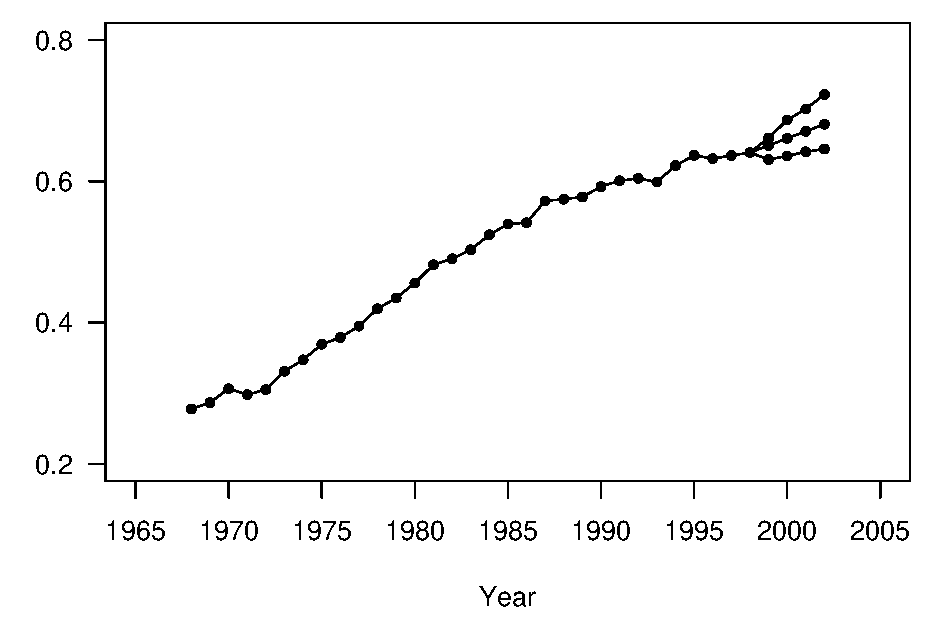
\includegraphics[width=.8\textwidth]{Chapter7Trend/LFPRFore.eps}
    \caption{\label{F7:LFPRFore} \small Time Series Plot of Labor Force Participation Rates
    with Forecast Values for 1999-2002. The middle series represent the point forecasts.
    The upper and lower series represent the upper and lower 95\% forecast intervals.
    Data for 1968-1998 represent actual values.}
  \end{center}
\end{figure}

\linejed

\subsubsection*{Identifying Stationarity}

We have seen how to do useful things, like forecasting, with random
walk models. But how do we identify a series as a realization from a
random walk? We know that the random walk is a special kind of
nonstationary model and so the first step is to examine a series and
decide whether or not it is stationary.

Stationarity quantifies the stability of a process. A process that
is strictly stationary has the same distribution over time, so we
should be able to take successive samples of modest size and show
that they have approximately the same distribution. For weak
stationary, the mean and variance are stable over time, so if one
takes successive samples of modest size, then we expect the mean
level and the variance to be roughly similar. To illustrate, when
examining time series plots, if you look at the first five, the next
five, the following five and so forth, successive samples, you
should observe approximately the same levels of averages and
standard deviations.

\marginparjed{A control chart is a time series plot with
superimposed reference lines called control limits. It is used is to
detect nonstationarity in a time series.}

\index{plots!control chart}

In quality management applications, this approach is quantified by
looking at \emph{control charts}.  A control chart is a useful
graphical device for detecting the lack of stationarity in a time
series. The basic idea is to superimpose reference lines called
\emph{control limits} on a time series plot of the data. These
reference lines help us visually detect trends in the data and
identify unusual points. The mechanics behind controls limits are
straightforward. For a given series of observations, calculate the
series mean and standard deviation, $\overline{y}$\ and $s_y$.
Define the
``upper control limit'' by $UCL=\overline{y}%
+3s_y$ and the ``lower control limit''\ by $LCL=\overline{y}-3s_y$.
Time series plots with these superimposed control limits are known
as control charts.

Sometimes the adjective \emph{retrospective} is associated with this
type of control chart. This adjective reminds the user that averages
and standard deviations are based on all the available data. In
contrast, when the control chart is used as an ongoing management
tool for detecting whether an industrial process is ``out of
control,'' a \emph{prospective control chart} may be more suitable.
Here, prospective merely means using only an early portion of the
process, that is ``in control,'' to compute the control limits.

\index{plots!Xbar chart}

A control chart that helps us to examine the stability of the mean
is the $Xbar$ chart. An $Xbar$ chart is created by combining
successive observations of modest size, taking an average over this
group, and then creating a control chart for the group averages. By
taking averages over groups, the variability associated with each
point on the chart is smaller than for a control chart for
individual observations. This allows the data analyst to get a
clearer picture of any patterns that may be evident in the mean of
the series.

\index{plots!$R$ chart}

A control chart that helps us examine the stability of the variability is
the $R$ chart. As with the $Xbar$ chart, we begin by forming successive
groups of modest size. With the $R$ chart, for each group we compute the
range, which is the largest minus the smallest observation, and then create
a control chart for the group ranges. The range is a measure of variability
that is simple to compute, an important advantage in manufacturing
applications.

\subsubsection*{Identifying Random Walks}

Suppose that you suspect that a series is nonstationary, how do
identify the fact that these are realizations of a random walk
model? Recall that the expected value of a random walk,
$\mathrm{E~}y_t=y_0+t\mu_c$, suggests that such a series follows a
linear trend in time. The variance of a random walk,
$\mathrm{Var~}y_t=t\sigma_c^2$, suggests that the variability of a
series gets larger as time $t$ gets large. First, a control chart
can help us to detect these patterns, whether they are of a linear
trend in time, increasing variability, or both.

\marginparjed{If the original data follows a random walk model, then
the differenced series follows a white noise process model.}

Second, if the original data follows a random walk model, then the
differenced series follows a white noise process model. If a random walk
model is a candidate model, you should examine the differences of the
series. In this case, the time series plot of the differences should be a
stationary, white noise process that displays no apparent patterns. Control
charts can help us to detect this lack of patterns.

Third, compare the standard deviations of the original series and
the differenced series. We expect the standard deviation of the
original series to be greater than the standard deviation of the
differenced series. Thus, if the series can be represented by a
random walk, we expect a substantial reduction in the standard
deviation when taking differences.

\linejed

\index{datasets!labor force participation rates}

\textbf{Example: Labor Force Participation Rates - Continued.} In
Figure \ref{F7:LFPR}, the series displays a clear upward trend
whereas the differences show no apparent trends over time. Further,
when computing differences of each series, it turned out
that%
\begin{equation*}
0.1197=SD(series)>SD(differences)=0.0101.
\end{equation*}
Thus, it seems reasonable to tentatively use a random walk as a
model of the labor force participation rate series.

In Chapter 8, we will discuss two additional identification devices.
These are scatter plots of the series versus a lagged version of the
series and the corresponding summary statistics called
\emph{autocorrelations}.

 \linejed
\subsubsection*{Random Walk versus Linear Trend in Time Models}

The labor force participation rate example could be represented
using either a random walk or a linear trend in time model. These
two models are more closely related to one another than is evident
at first glance. To see this relationship, recall that the linear
trend in time model can be written as
\begin{equation}\label{E7:7}
y_t = \beta_0 + \beta_1 t + \varepsilon_t,
\end{equation}
where $\{\varepsilon_t\}$ is a white noise process. If $\{y_t\}$ is
a random walk, then it can be modeled as a partial sum as in
equation (\ref{E7:6}). We can also decompose the white noise process
into a mean $\mu _c$ plus another white noise process, that is, $c_t
= \mu_c + \varepsilon_t$. Combining these two ideas, a random walk
model can be written as

\begin{equation} \label{E7:8}
y_t = y_0 + \mu_c t + u_t
\end{equation}
where $u_t = \sum_{j=1}^{t} \varepsilon_j$. Comparing equations
(\ref{E7:7}) and (\ref{E7:8}), we see that the two models are
similar in that the deterministic portion is a linear function of
time. The difference is in the error component. The error component
for the linear trend in time model is a stationary, white noise
process. The error component for the random walk model is
nonstationary because it is the partial sum of white noise
processes. That is, the error component is also a random walk. Many
introductory treatments of the random walk model focus on the ``fair
game'' example and ignore the drift term $\mu_c$. This is
unfortunate because the comparison between the random walk model and
the linear trend in time model is not as clear when the parameter
$\mu_c$ is equal to zero.

\section{Filtering to Achieve Stationarity}


A \emph{filter} is a procedure for reducing observations to white
noise. In regression, we accomplished this by simply subtracting the
regression function from the observations, that is, $y_i - (\beta_0
+ \beta_1 x_{1i} + \ldots + \beta_k x_{ki})=\varepsilon_i$.
Transformation of the data is another device for filtering that we
introduced in Chapter 1 when analyzing cross-sectional data. We
encountered another example of a filter in Section
\ref{S7:RandomWalk}. There, by taking differences of observations,
we reduced a random walk series to a white noise process.

\marginparjed{A filter is a procedure for reducing observations to
white noise.}\index{time series terms and concepts!filter}

An important theme of this text is to use an iterative approach for
fitting models to data. In particular, in this chapter we discuss
techniques for reducing a sequence of observations to a stationary
series. By definition, a stationary series is stable and hence is
far easier to forecast than an unstable series. This stage,
sometimes known as \emph{pre-processing} the data, generally
accounts for the most important sources of trends in the data. The
next chapter will present models that account for subtler trends in
the data.

\subsubsection*{Transformations}

When analyzing longitudinal data, transformation is an important
tool used to filter a data set. Specifically, using a logarithmic
transformation tends to shrink ``spread out'' data. This feature
gives us an alternative method to deal with a process where the
variability appears to grow with time. Recall the first option
discussed is to posit a random walk model and examine differences of
the data. Alternatively, one may take a logarithmic transform that
helps to reduce increasing variance through time.

Further, from the random walk discussion, we know that if both the
series variance and log series variance increase through time, the
differences of the log transform might handle this increasing
variability. Differences of natural logarithms are particularly
pleasing because they can be interpreted as \emph{proportional
changes}. To see this, define $pchange_t=(y_t/y_{t-1})-1$. Then,
\begin{equation*}
\ln y_t-\ln y_{t-1} = \ln \left( \frac{y_t}{y_{t-1}}\right) = \ln
\left( 1+pchange_t\right) \approx pchange_t.
\end{equation*}
Here we use the Taylor series approximation $\ln (1+x) \approx x$
that is appropriate for small values of $|x|$.

\linejed

\index{datasets!Standard and Poor's quarterly index}

\textbf{Example: Standard and Poor's Composite Quarterly
Index.}\ecaptionjed{Standard and Poor's Composite Quarterly Index}
An important task of a financial analyst is to quantify costs
associated with future cash flows. We consider here funds invested
in a standard measure of overall market performance, the Standard
and Poor's (S\&P) 500 Composite Index. The goal is to forecast the
performance of the portfolio for discounting of cash flows.

In particular, we examine the S\&P Composite Quarterly Index for the
years 1936 to 2007, inclusive. By today's standards, this period may
not be the most representative because the Depression of the 1930's
is included. The motivation to analyze these data is from the
Institute of Actuaries ``Report of the Maturity Guarantees Working
Party'' (1980) who analyzed the series from 1936 to 1977, inclusive.
This paper studied the long term behavior of investment returns from
an actuarial viewpoint. We complement that work by showing how
graphical techniques can suggest a useful transformation for
reducing the data to a stationary process.

The data are shown in Figure \ref{F7:SandPTS}. From the original
index values in the upper left-hand panel, we see that the mean
level and variability increases with time. This pattern clearly
indicates that the series is nonstationary.

From our discussions in Sections \ref{S7:Trends} and
\ref{S7:RandomWalk}, a candidate model that has these properties is
the random walk. However, the time series plot of the differences,
in upper right-hand panel of Figure \ref{F7:SandPTS}, still
indicates a pattern of variability increasing with time. The
differences are not a white noise process so the random walk is not
a suitable model for the S \& P 500 Index.

An alternative transformation is to consider logarithmic values of
the series. The time series plot of logged values, presented in
lower left-hand panel of Figure \ref{F7:SandPTS}, indicates the the
mean level of the series increases over time and is not level. Thus,
the logarithmic index is not stationary.

Yet another approach is to examine differences of the logarithmic
series. This is especially desirable when looking at indices, or
\textquotedblleft breadbaskets,\textquotedblright\ because the
difference of logarithms can be interpreted as proportional changes.
From the final time series plot, in the lower right-hand panel of
Figure \ref{F7:SandPTS}, we see that there are fewer discernible
patterns in the transformed series, the difference of logs. This
transformed series seems to be stationary. It is interesting to note
that there seems to be a higher level of volatility at the beginning
of the series. This type of changing volatility is more difficult to
model and has recently been the subject of considerable attention in
the financial economics literature (see, for example, Hardy, 2003).


\begin{figure}[htp]
  \begin{center}
    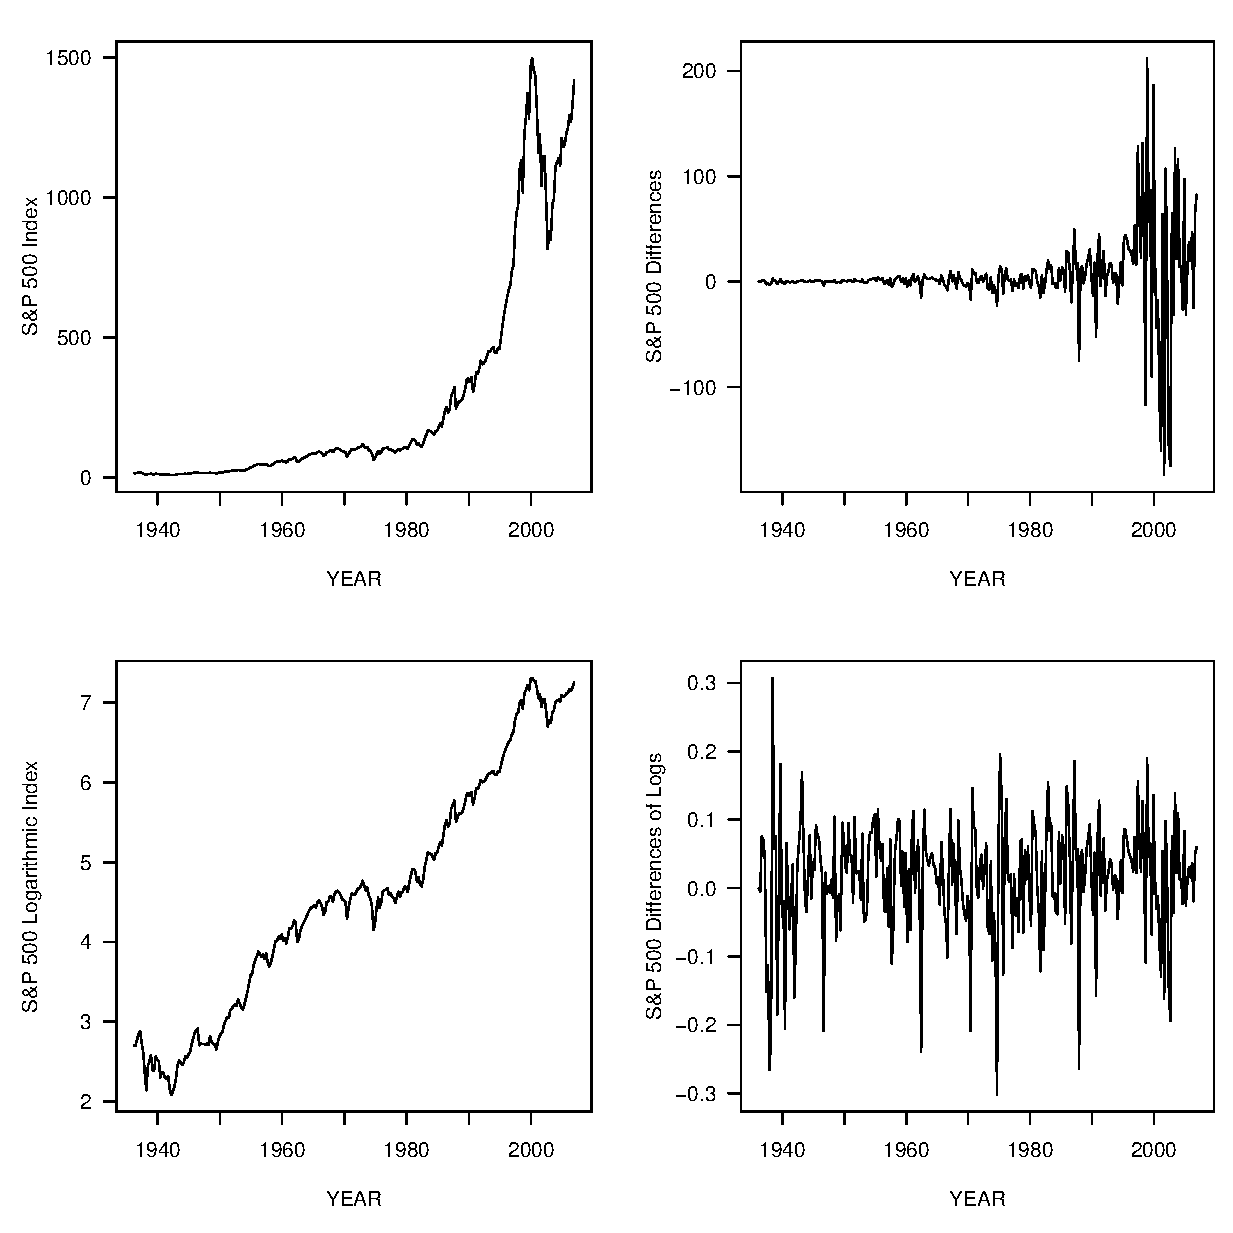
\includegraphics[width=1\textwidth]{Chapter7Trend/SandPTS.eps}
    \caption{\label{F7:SandPTS} \small Time Series Plots of the S \& P 500 Index. The upper
left-hand panel shows the original series that is nonstationary in
the mean and in the variability. The upper right-hand panel shows
the differences in the series that is nonstationary in the
variability. The lower left-hand panel shows the logarithmic index
that is nonstationary in the mean. The lower right hand panel shows
the differences of the logarithmic index that appears to be
stationary in the mean and in the variability.}
  \end{center}
\end{figure}

\linejed

\section{Forecast Evaluation}

Judging the accuracy of forecasts is important when modeling time series
data. In this section, we present forecast evaluation techniques that:

\begin{itemize}
\item Help detect recent unanticipated trends or patterns in the data.

\item Are useful for comparing different forecasting methods.

\item Provide an intuitive and easy to explain method for evaluating the
accuracy of forecasts.
\end{itemize}

In the first five sections of Chapter 7, we presented several techniques for
detecting patterns in residuals from a fitted model. Measures that summarize
the distribution of residuals are called \emph{goodness-of-fit statistics}.
As we saw in our study of cross-sectional models, by fitting several
different models to a data set, we introduce the possibility of overfitting
the data. To address this concern, we will use \emph{out-of-sample validation%
} techniques, similar to those introduced in Section 6.5.

To perform an out-of-sample validation of a proposed model, ideally
one would develop the model on a data set and then corroborate the
model's usefulness on a second, independent data set. Because two
such ideal data sets are rarely available, in practice we can split
a data set into two subsamples, a \emph{model development subsample}
and a \emph{validation subsample}. For longitudinal data, the
practice is to use the beginning part of the series, the first $T_1$
observations, to develop one or more candidate models. The latter
part of the series, the last $T_2=T-T_1$ observations, are used to
evaluate the forecasts. For example, we might have ten years of
monthly data so that $T=120$. It would be reasonable to use the
first eight years of data to develop a model and the last two years
of data for validation, yielding $T_1=96$ and $T_2=24$.

Thus, observations $y_1,\ldots , y_{T_1}$ are used to develop a
model. From these $T_1$ observations, we can determine the
parameters of the candidate model. Using the fitted model, we can
determine fitted values for the model validation subsample for $t =
T_1 + 1,T_1+2, \ldots, T_1+T_2$. Taking the difference between the
actual and fitted values yield one-step forecast residuals, denoted
by $e_t=y_t-\widehat{y}_t$. These forecast residuals are the basic
quantities that we will use to evaluate and compare forecasting
techniques.

To compare models, we use a four-step process similar to that described in
Section 6.5, described as follows.

\boxedjed

\textit{Out-of-Sample Validation Process}

\begin{compactenum}[1.]
\item Divide the sample of size $T$ into two subsamples, a model development
subsample ($t=1,\ldots,T_1$) and a model validation subsample
($t=T_1+1, \ldots, T_1 + T_2$).

\item Using the model development subsample, fit a candidate model to the
data set $t=1,\ldots,T_1$.

\item Using the model created in Step 2 and the dependent variables up to
and including $t-1$, forecast the dependent variable
$\widehat{y}_t$, where $t=T_1+1, \ldots, T_1+T_2$.

\item Use actual observations and the fitted values computed in Step 3 to
compute one-step forecast residuals, $e_t = y_t- \widehat{y}_t$, for
the model validation subsample. Summarize these residuals with one
or more comparison statistics, described below.
\end{compactenum}

Repeat Steps 2 through 4 for each of the candidate models. Choose
the model with the smallest set of comparison statistics.


\end{boxedminipage}

\bigskip

Out-of-sample validation can be used to compare the accuracy of forecasts
from virtually any forecasting model. As we saw in Section 6.5, we are not
limited to comparisons where one model is a subset of another, where the
competing models use the same units for the response, and so on.

There are several statistics that are commonly used to compare
forecasts.

\boxedjed

\textit{Commonly Used Statistics for Comparing Forecasts}

1. The \emph{mean error statistic}, defined by%
\begin{equation*}
ME=\frac{1}{T_2}\sum_{t=T_1+1}^{T_1+T_2}e_t.
\end{equation*}
This statistic measures recent trends that are not anticipated by the model.

2. The \emph{mean percent error}, defined by
\begin{equation*}
MPE=\frac{100}{T_2}\sum_{t=T_1+1}^{T_1+T_2}\frac{e_t}{y_t}.
\end{equation*}
This statistic is also a measure of trend, but examines error relative to
the actual value.

3. The \emph{mean square error}, defined by%
\begin{equation*}
MSE=\frac{1}{T_2}\sum_{t=T_1+1}^{T_1+T_2}e_t^2.
\end{equation*}
This statistic can detect more patterns than $ME$. It is the same as
the cross-sectional $SSPE$ statistic, except for the division by
$T_2$.

4. The \emph{mean absolute error}, defined by
\begin{equation*}
MAE=\frac{1}{T_2}\sum_{t=T_1+1}^{T_1+T_2}|e_t|.
\end{equation*}
Like $MSE$, this statistic can detect more than trend patterns than $ME$.
The units of $MAE$ are the same as the dependent variable.

5. The \emph{mean absolute percent error}, defined by%
\begin{equation*}
MAPE=\frac{100}{T_2}\sum_{t=T_1+1}^{T_1+T_2}|\frac{e_t}{y_t}|.
\end{equation*}%
Like $MAE$, this statistic can detect more than trend patterns. Like $MPE$,
it examines error relative to the actual value.

\end{boxedminipage}

\bigskip

\linejed

\index{datasets!labor force participation rates}

\textbf{Example: Labor Force Participation Rates - Continued. }We
can use out-of-sample validation measures to compare two models for
the $LFPR$s; the linear trend in time model and the random walk
model. For this illustration, we examined the labor rates for years
1968 through 1994, inclusive. This corresponds to $T_1 = 27$
observations defined in Step 1. Data were subsequently gathered on
rates for 1995 through 1998, inclusive, corresponding to $T_2 = 4$
for out-of-sample validation. For Step 2, we fit each model using
$t=1,\ldots,27$, earlier in this chapter. For Step 3, the one-step
forecasts are:

\begin{equation*}
\widehat{y}_t = 0.2574 + 0.0145t
\end{equation*}%
and%
\begin{equation*}
\widehat{y}_t = y_{t-1} + 0.0132
\end{equation*}
for the linear trend in time and the random walk models,
respectively. For Step 4, Table \ref{T7:ForecastComparison}
summarizes the forecast comparison statistics. Based on these
statistics, the choice of the model is clearly the random walk.

\scalefont{0.9}
\begin{table}[h]
\caption{\label{T7:ForecastComparison} Out of Sample Forecast
Comparison}
\begin{center}
\begin{tabular}{c|ccccc}
\hline & $ME$ & $MPE$ & $MSE$ & $MAE$ & $MAPE$ \\ \hline
\multicolumn{1}{l|}{Linear trend in time model} & -0.0488 & -0.0766
& 0.0026
& 0.0488 & 0.0766 \\
\multicolumn{1}{l|}{Random walk model} & -0.0007 & ~0.0012 & 0.0001
& 0.0115 & 0.0180 \\ \hline
\end{tabular}\end{center}\end{table}
\scalefont{1.1111}

\linejed



\section{Further Reading and References}

For many years, actuaries in North America were introduced to time
series analysis from Miller and Wichern (1977), Abraham and Ledolter
(1983) and Pindyck and Rubinfeld (1991). A more recent book-long
introduction is Diebold (2004). Diebold contains a brief
introduction to regime-switching models.


Because of the difficulties regarding their specification and
limited forecasting use, we do not explore causal models further in
this text. For more details on causal models, the interested reader
is referred to Pindyck and Rubinfeld (1991).

\bigskip

\textbf{Chapter References}

\begin{multicols}{2}

\scalefont{0.9}


``Report of the Maturity Guarantees Working Party'' (1980).
\textit{Journal of the Institute of Actuaries} 107, pp. 103-213.

Abraham, Bovas and  Johannes Ledolter (1983). \textit{Statistical
Methods for Forecasting}. John Wiley \& Sons, New York.

Diebold, Francis X. (2004). \textit{Elements of Forecasting}, Third
Edition. Thompson South-Western, Mason, OH.

Frees, Edward W. (2006). Forecasting of labor force participation
rates. \emph{The Journal of Official Statistics} 22(3), 453-485.

Fullerton, Howard N., Jr. (1999). Labor force projections to 2008:
steady growth and changing composition. \textit{Monthly Labor
Review}, November, pp. 19-32.

Granger, Clive W. J and P. Newbold (1974). Spurious regressions in
econometrics. \textit{Journal of Econometrics} 2, 111-120.

Hardy, Mary (2001). A regime-switching model of long-term stock
returns. \emph{North American Actuarial Journal} 5(2), 41-53.

Hardy, Mary (2003). \emph{Investment Guarantees: Modeling and Risk
Management for Equity-Linked Life Insurance}. John Wiley \& Sons,
New York.

Miller, Robert B. and Dean W. Wichern (1977). \emph{Intermediate
Business Statistics: Analysis of Variance, Regression and Time
Series}. Holt, Rinehart and Winston, New York.

Pindyck, R.S. and D.L. Rubinfeld (1991). \textit{Econometric Models
and Economic Forecasts,} Third Edition, McGraw-Hill, New York.

\scalefont{1.1111}

\end{multicols}

\section{Exercises}

\scalefont{0.90}
\begin{exercises}

\item Consider a random walk $\{y_t \}$ as the partial sum of a white noise process $\{ c_t \}$ with
mean $\mathrm{E}~c_t= \mu_c$ and variance $\mathrm{Var}~c_t =
\sigma_c^2$. Use equation (\ref{E7:6}) to show

a.  $\mathrm{E}~y_t= y_0 + t \mu_c$, where $y_0$ is the initial
value and

b.  $\mathrm{Var}~y_t= t \sigma_c^2$.

\item Consider a random walk $\{y_t \}$ as the partial sum of a white noise process $\{ c_t
\}$.

a. Show that the $l$-step forecast error is
$y_{T+l}-\widehat{y_{T+l}} = \sum_{j=1}^l (c_{T+j} - \bar{c} ).$

b. Show that the approximate variance of the $l$-step forecast error
is $l \sigma_c^2.$



\empexjed{EuroExchange}\index{datasets!Euro exchange rates}

\item \textbf{Euro Exchange Rates}. The exchange rate that we consider is the amount of Euros that one
can purchase for one US dollar. We have $T=699$ daily observations
from the period April 1, 2005 through January 8, 2008. These data
were obtained from the Federal Reserve (H10 report). \emph{Source}:
Federal Reserve Bank of New York. Note: The data are based on noon
buying rates in New York from a sample of market participants and
they represent rates set for cable transfers payable in the listed
currencies. These are also the exchange rates required by the
Securities and Exchange Commission for the integrated disclosure
system for foreign private issuers.


\begin{figure}[htp]
  \begin{center}
   \includegraphics[width=1\textwidth,angle=0,scale=0.6]{Chapter7Trend/EuroPlot1.eps}
   \caption{\label{Ex:EuroPlot1} \small Time series plot of the Euro exchange rate.}
  \end{center}
\end{figure}


a. Figure \ref{Ex:EuroPlot1} is a time series plot of the Euro
exchange rate.

a(i). Define the concept of a stationary time series.

a(ii). Is the EURO series stationary? Use your definition in part
a(i) to justify your response.

b. Based on an inspection of Figure \ref{Ex:EuroPlot1} in part (a),
you decide to fit a quadratic trend model of the data. Figure
\ref{Ex:EuroPlot2} superimposes the fitted value on a plot of the
series.


\begin{figure}[htp]
  \begin{center}
   \includegraphics[width=1\textwidth,angle=0,scale=0.6]{Chapter7Trend/EuroPlot2.eps}
   \caption{\label{Ex:EuroPlot2} \small  Quadratic fitted curve superimposed on the Euro exchange rate.}
  \end{center}
\end{figure}

b(i). Cite several basic regression statistics that summarize the
quality of the fit.

b(ii). Briefly describe any residual patterns that you observe in
Figure \ref{Ex:EuroPlot2}.

b(iii). Here, TIME varies from $1, 2, \ldots, 699$. Using this model
calculate the three-step forecast corresponding to TIME = 702.


\bigskip

c. To investigate a different approach, DIFFEURO, calculate the
difference of EURO. You decide to model DIFFEURO as a white noise
process.

c(i).  What is the name for the corresponding model of EURO?

c(ii). The most recent value of EURO is $EURO_{699} = 0.6795$. Using
the model identified in part c(i), provide a three-step forecast
corresponding to TIME = 702.

c(iii).  Using the model identified in part c(i) and the point
forecast in part c(ii), provide the corresponding 95\% prediction
interval for $EURO_{702}$.



\end{exercises}
\scalefont{1.1111}

\setcounter{chapter}{7}
\chapter{Autocorrelations and Autoregressive Models}
{\small \textit{Chapter Preview}. This chapter continues our study
of time series data. Chapter 7 introduced techniques for determining
major patterns that provide a good first step for forecasting.
Chapter 8 provides techniques for detecting subtle trends in time
and models to accommodate these trends. These techniques detect and
model relationships between the current and past values of a series
using regression concepts.}

\section{Autocorrelations}\label{S8:Autocorrs}

\empexjed{InflationBond}

\subsubsection*{Application: Inflation Bond Returns}\ecaptionjed{Inflation Bond Returns}
\index{datasets!TIPS - inflation bond returns}

To motivate the methods introduced in this chapter, we work in the
context of the inflation bond return series. Beginning in January of
2003, the US Treasury Department established an inflation bond index
that summarizes the returns on long-term bonds offered by the
Treasury Department that are inflation-indexed. For a Treasury
inflation protected security (TIPS), the principal of the bond is
indexed by the (three month lagged) value of the (non-seasonally
adjusted) consumer price index. The bond then pays a semi-annual
coupon at a rate determined at auction when the bond is issued. The
index that we examine is the unweighted average of bid yields for
all TIPS with remaining terms to maturity of 10 or more years.

Monthly values of the index from January 2003 through March 2007 are
considered, for a total of $T=51$ returns. A time series plot of the
data is presented in Figure \ref{F8:InfBondTS}. This plot suggests
that the series is stationary and so it is useful to examine the
distribution of the series through summary statistics that appear in
Table \ref{T8:InfBondSumStats}.

\begin{figure}[htp]
  \begin{center}
     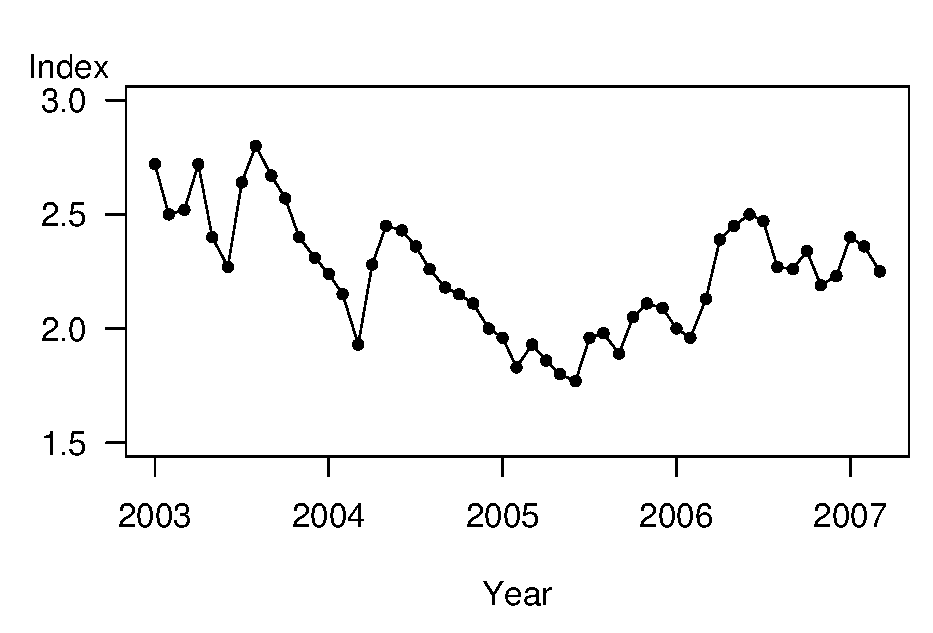
\includegraphics[width=.68\textwidth]{Chapter8AutoReg/InfBondTS.eps}
    \caption{\label{F8:InfBondTS} \small Time Series Plot of the Inflation Bond
    Index. Monthly values over January 2003 to March 2007, inclusive.}
  \end{center}
\end{figure}

\bigskip

\begin{table}[h]
\caption{\label{T8:InfBondSumStats} Summary Statistics of the
Inflation Bond Index}
\begin{center}
\begin{tabular}{lccccc}
\hline
&  &  & Standard &  &  \\
Variable & Mean & Median & Deviation & Minimum & Maximum \\ \hline
INDEX & 2.245 & 2.26 & 0.259 & 1.77 & 2.80 \\
\hline ~~~\emph{Source}: US Treasury
\end{tabular}\end{center}\end{table}

\bigskip

Our goal is detect patterns in the data and provide models to
represent these patterns. Although Figure \ref{F8:InfBondTS} shows a
stationary series with no major tendencies, a few subtle patterns
are evident. Beginning in mid 2003 and then in the beginning of
2004, we see large increases followed by a series of declines in the
index. Beginning in 2005, a pattern of increase with some cyclical
behavior seems to be occurring. Although it is not clear what
economic phenomenon these patterns represent, they are not what we
would expect to see with a white noise process. For a white noise
process, a series may increase or decrease randomly from one period
to the next, producing a non-smooth, ``jagged'' series over time.

To help understand these patterns, Figure \ref{F8:InfBondLag}
presents a scatter plot of the series ($y_t$) versus its lagged
value ($y_{t-1}$). Because this is a crucial step to understanding
this chapter, Table \ref{T8:InfBondIndex} presents a small subset of
the data so that you can see exactly what each point on the scatter
plot represents. Figure \ref{F8:InfBondLag} shows a strong
relationship between $y_t$ and $y_{t-1}$; we will model this
relationship in the next section.

\begin{figure}[htp]
  \begin{center}
    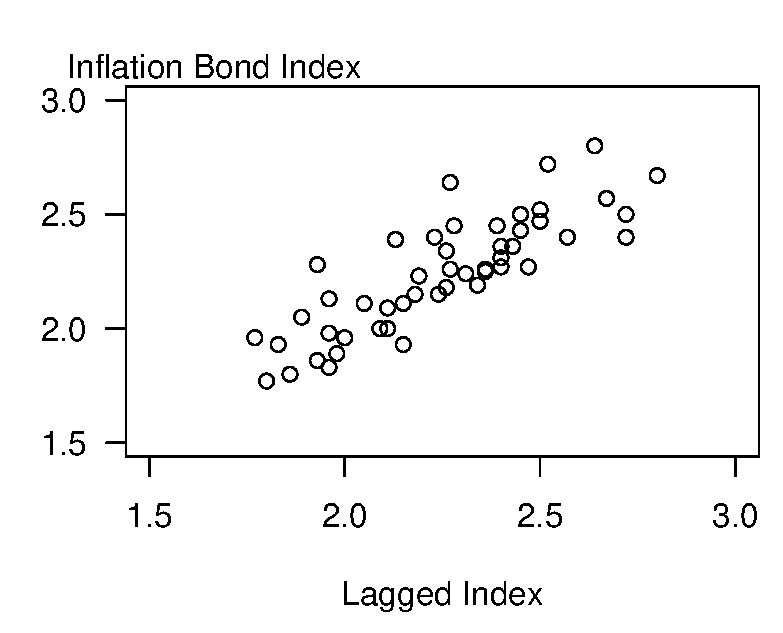
\includegraphics[width=.7\textwidth]{Chapter8AutoReg/InfBondLag.eps}
    \caption{\label{F8:InfBondLag} \small Inflation
Bond versus Lagged Value. This scatter plot reveals a linear
relationship between the index and its lagged value.}
  \end{center}
\end{figure}


\begin{table}[h]
\caption{\label{T8:InfBondIndex} Index and Lagged Index for the
First Five of $T=51$ Values}
\begin{center}
\begin{tabular}{l|rrrrr}
\hline
$t$ & 1~~ & 2~~ & 3~~ & 4~~ & 5~~ \\
Index ($y_t$) & 2.72 & 2.50 &  2.52 &  2.72 & 2.40 \\
Lagged Index ($y_{t-1}$) & * &  2.72   &  2.50   &  2.52  & 2.72
\\ \hline
\end{tabular}\end{center}\end{table}


\bigskip

\subsubsection*{Autocorrelations}\index{correlation coefficients!autocorrelations}

Scatter plots are useful because they graphically display nonlinear,
as well as linear, relationships between two variables. As we
established in Chapter 2, correlations can be used to measure the
linear relation between two variables. Recall that when dealing with
cross-sectional data, we summarized
relations between \{$y_t$\} and \{$x_t$\} using the correlation statistic%
\begin{equation*}
r = \frac{1}{(T-1)s_{x}s_y} \sum_{t=1}^{T} \left( x_t -
\overline{x}\right) \left( y_t-\overline{y} \right) .
\end{equation*}
We now mimic this statistic using the series \{$y_{t-1}$\} in place
of \{$x_t$\}. With this replacement, use $\overline{y}$\ in place of
$\overline{x}$\ and, for the denominator, use $s_y$ in place of
$s_x$. With this last substitution, we have $(T-1) s_y^2 =
\sum_{t=1}^{T}(y_t-\overline{y} )^2$. Our resulting correlation
statistic is

\begin{equation*}
r_1 = \frac{\sum_{t=2}^{T} \left( y_{t-1}-\overline{y}\right) \left(
y_t- \overline{y}\right) }{\sum_{t=1}^{T} (y_t-\overline{y})^2}.
\end{equation*}
This statistic is referred to as an \emph{autocorrelation}, that is,
a correlation of the series upon itself. This statistic summarizes
the linear relationship between \{$y_t$\} and \{$y_{t-1}$\}, that
is, observations that are one time unit apart. It will also be
useful to summarize the linear relationship between observations
that are $k$ time units apart, \{$y_t$\} and \{$y_{t-k}$\}, as
follows.\bigskip

\boxedjed

\textbf{Definition.} \ The \emph{lag k autocorrelation statistic} is
\begin{equation*}
r_k = \frac{\sum_{t=k+1}^{T}\left( y_{t-k}-\overline{y}\right) \left( y_t-%
\overline{y}\right) }{\sum_{t=1}^{T}(y_t-\overline{y})^2},
~~~~k=1,2, \ldots
\end{equation*}\index{time
series statistics!lag $k$ autocorrelation}


\end{boxedminipage}
\bigskip

Properties of autocorrelations are similar to correlations. Just as
with the usual correlation statistic $r$, the denominator,
$\sum_{t=1}^{T}(y_t - \overline{y})^2$, is always nonnegative and
hence does not change the sign of the numerator. We use this
rescaling device so that $r_k$ always lies within the interval [-1,
1]. Thus, when we interpret $r_k$, a value near -1, 0 and 1, means,
respectively, a strong negative, near null or strong positive
relationship between $y_t$ and $y_{t-k}$. If there is a positive
relationship between \ $y_t$ and $y_{t-1}$, then $r_1 > 0$ and the
process is said to be \emph{positively autocorrelated}. For example,
in Table \ref{T8:InfBondAutocorrs} are the first five
autocorrelations of the inflation bond series. These
autocorrelations indicate that there is a positive relationship
between adjacent observations.

\begin{table}[h]
\caption{\label{T8:InfBondAutocorrs} Autocorrelations for the
Inflation Bond Series}
\begin{center}
\begin{tabular}{c|ccccc}
\hline
Lag $k$ & 1 & 2 & 3 & 4 & 5 \\
Autocorrelation $r_k$ & 0.814 & 0.632 & 0.561 & 0.447 & 0.267 \\
\hline
\end{tabular}\end{center}\end{table}


\section{Autoregressive Models of Order One}
\index{time series models!autoregressive model of order one,
$AR$(1)}


\subsubsection*{Model Definition and Properties}

In Figure \ref{F8:InfBondLag} we noted the strong relationship
between the immediate past and current values of the inflation bond
index. This suggests using $y_{t-1}$ to explain $y_t$ in a
regression model. Using previous values of a series to predict
current values of a series is termed, not surprisingly, an
\emph{autoregression}. When only the immediate past is used as a
predictor, we use the following model.\bigskip

\boxedjed

\textbf{Definition.} \ The \emph{autoregressive model of order one}, denoted
by $AR(1)$, is written as%
\begin{equation}\label{E8:AR1}
y_t = \beta_0 + \beta_1 y_{t-1} + \varepsilon_t,\text{ \ \ \ \ \ \ \
\ } t=2,\ldots,T,
\end{equation}
where \{$\varepsilon_t$\} is a white noise process such that
$\mathrm{Cov}(\varepsilon_{t+k}, y_t)=0$ for $k>0$ and $\beta_0$ and
$\beta_1$ are unknown parameters.

\end{boxedminipage}
\bigskip

In the $AR$(1) model, the parameter $\beta_0$ may be any fixed
constant. However, the parameter $\beta_1$ is restricted to be
between -1 and 1. By making this restriction, it can be established
that the $AR$(1) series \{$y_t$\} is stationary. Note that if
$\beta_1 = 1$, then the model is a random walk and hence is
nonstationary. This is because, if $\beta_1 = 1$, then equation
(\ref{E8:AR1}) may be rewritten as
\begin{equation*}
y_t - y_{t-1} = \beta_0 + \varepsilon_t.
\end{equation*}
If the difference of a series forms a white noise process, then the series
itself must be a random walk.

\marginparjed{For stationarity in the $AR$(1) model, we require
$|\beta_1|<1.$}

The equation (\ref{E8:AR1}) is useful in the discussion of model
properties. We can view an $AR$(1) model as a generalization of both
a white noise process and a random walk model. If $\beta_1=0$, then
equation (\ref{E8:AR1}) reduces to a white noise process. If
$\beta_1 = 1,$ then equation (\ref{E8:AR1}) is a random walk.

A stationary process where there is a linear relationship between
$y_{t-2}$ and $y_t$ is said to be \emph{autoregressive of order 2},
and similarly for higher order processes. Discussion of higher order
processes is in Section \ref{S8:BoxJenkins}.

\subsubsection*{Model Selection}

When examining the data, how does one recognize that an
autoregressive model may be a suitable candidate model? First, an
autoregressive model is stationary and thus a control chart is a
good device to examine graphically the data to search for stability.
Second, adjacent realizations of an $AR$(1) model should be related;
this can be detected visually by a scatter plot of current versus
immediate past values of the series. Third, we can recognize an
$AR$(1) model through its autocorrelation structure, as follows.

A useful property of the $AR$(1) model is that the correlation
between points $k$ time units apart turns out to be $\beta_1^{k}$.
Stated another way,
\begin{equation}\label{E8:AR1Autocorrelations}
\rho_k = \mathrm{Corr}(y_t,y_{t-k}) =
\frac{\mathrm{Cov}(y_t,y_{t-k})}{\sqrt{\mathrm{Var}(y_t)\mathrm{Var}(y_{t-k})}}
= \frac{\mathrm{Cov}(y_t,y_{t-k})}{\sigma_y^2} = \beta_1^k.
\end{equation}
\marginparjed{For a (stationarity) $AR$(1) model, $\rho_k =\beta_1
^k .$}


\noindent The first two equalities are definitions and the third is
due to the stationarity. The reader is asked to check the fourth
equality in the exercises. Hence, the absolute values of the
autocorrelations of an $AR$(1) process become smaller as the lag
time $k$ increases. In fact, they decrease at a geometric rate. We
remark that for a white noise process, we have $\beta_1 = 0$, and
thus $\rho_k$ should be equal to zero for all lags $k$.

As an aid in model identification, we use the idea of matching the
observed autocorrelations $r_k$ to quantities that we expect from
the theory, $\rho_k$. For white noise, the sample autocorrelation
coefficient should be approximately zero for each lag $k$. Even
though $r_k$ is algebraically bounded by -1 and 1, the question
arises, how large does $r_k$ need to be, in absolute value, to be
considered significantly different from zero? The answer to this
type of question is given in terms of the statistic's standard
error. Under the hypothesis of no autocorrelation, a good
approximation to the standard error of the lag $k$ autocorrelation
statistic is
\begin{equation*}
se(r_k) = \frac{1}{\sqrt{T}}.
\end{equation*}
Our rule of thumb is that if $r_k$ exceeds $2 \times se(r_k)$ in
absolute value, it may be considered to be significantly non-zero.
This rule is based on a 5\% level of significance.

\linejed \index{datasets!TIPS - inflation bond returns}

\textbf{Example: Inflation Index Bonds - Continued.} Is a white
noise process model a good candidate to represent this series? The
autocorrelations are given in Table \ref{T8:InfBondIndex}. For a
white noise process model, we expect each autocorrelation $r_k$ to
be close to zero but note that, for example, $r_1=0.814$. Because
there are $T=51$ returns available, the approximate standard error
of each autocorrelation is
\begin{equation*}
se(r_k) = \frac{1}{\sqrt{51}} = 0.140.
\end{equation*}
Thus, $r_1$ is 0.814 / 0.140 = 5.81 standard errors above zero.
Using the normal distribution as a reference base, this difference
is significant, implying that a white noise process is not a
suitable candidate model.

Is the autoregressive model of order one a suitable choice? Well,
because $\rho_k$ = $\beta_1^{k}$, a good estimate of
$\beta_1$=$\rho_1$ is $r_1=0.814$. If this is the case, then under
the $AR$(1) model, another estimate of $\rho_k$ is $(0.814)^{k}$.
Thus, we have two estimates of $\rho_k$; (i) $r_k$, an empirical
estimate that does not depend on a parametric model and (ii)
$(r_1)^{k}$, that depends on the $AR$(1) model. To illustrate, see
Table \ref{T8:InfBondAutoEstimated}.



\begin{table}[h]
\begin{center}
\caption{\label{T8:InfBondAutoEstimated} Comparison of Empirical
Autocorrelations to Estimated under the $AR$(1) model}
\begin{tabular}{l|ccccc}
\hline
Lag $k$ & 1 & 2 & 3 & 4 & 5 \\
Estimated $\rho_k$ under the $AR$(1) model & $0.814$ & $(0.814)^2$ & $%
(0.814)^{3}$ & $(0.814)^{4}$ & $(0.814)^{5}$ \\
&  & \multicolumn{1}{r}{$=.66$} &
\multicolumn{1}{r}{$=.54$} & \multicolumn{1}{r}{$=.44$} & \multicolumn{1}{r}{%
$=.36$} \\
Autocorrelation $r_k$ & $0.814$ & $0.632$ & $0.561$ & $0.447$ & $0.267$ \\
\hline
\end{tabular}\end{center}\end{table}


\bigskip

Given that the approximate standard error is $se(r_k) = 0.14$, there
seems to be a good match between the two sets of autocorrelations.
Because of this match, in Section \ref{S8:Estimation} we will
discuss how to fit the $AR$(1) model to this set of data.

\linejed

\subsubsection*{Meandering Process}\index{time series terms and concepts!meandering
process}

Many processes display the pattern of adjacent points being related
to one another. Thinking of a process evolving as a river, Roberts
(1991) picturesquely describes such processes as \emph{meandering}.
To supplement this intuitive notion, we say that a process is
meandering if the lag one autocorrelation of the series is positive.
For example, from the plots in Figures \ref{F8:InfBondTS} and
\ref{F8:InfBondLag}, it seems clear that the Inflation Bond Index is
a good example of a meandering series. Indeed, an $AR$(1) model with
a positive slope coefficient is a meandering process.

What about the case when the slope coefficient approaches one,
resulting in a random walk? Consider the Hong Kong Exchange Rates
example given in Chapter 7. Although introduced as a quadratic trend
in time model, an exercise shows that the series can more
appropriately be modeled as a random walk. It seems clear that any
point in the process is highly related to each adjacent point in the
process. To emphasize this point, Figure \ref{F8:HKLag} shows a
strong linear relationship between the current and immediate past
value of exchange rates. Because of the strong linear relationship
in Figure \ref{F8:HKLag}, we will use the terminology ``meandering
process'' for a data set that may be modeled using a random walk.

\begin{figure}[htp]
  \begin{center}
   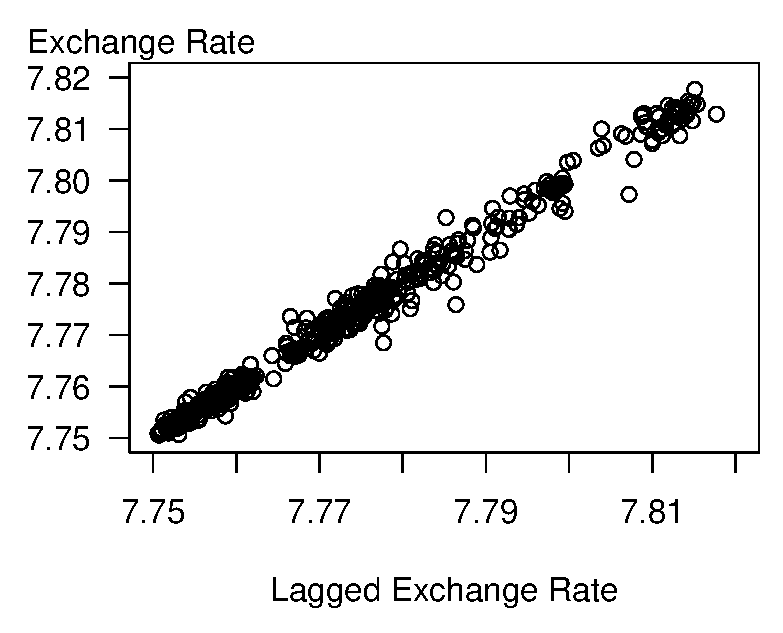
\includegraphics[width=.5\textwidth]{Chapter8AutoReg/HKLag.eps}
    \caption{\label{F8:HKLag} \small Hong Kong Daily Exchange Rates versus Lagged Values.}
  \end{center}
\end{figure}

\section{Estimation and Diagnostic Checking}\label{S8:Estimation}

Having identified a tentative model, the task now at hand is to
estimate values of $\beta_0$ and $\beta_1$. In this section, we use
the \emph{method of conditional least squares} to determine the
estimates, denoted as $b_0$ and $b_1$, respectively. This approach
is based on the least squares method that was introduced in Section
2.1. Specifically, we now use the least squares to find estimates
that best fit an observation \emph{conditional} on the previous
observation.

Formulas for the conditional least squares estimates are determined
from the usual least squares procedures, using the lagged value of
$y$ for the explanatory variable. It is easy to see that conditional
least squares estimates are closely approximated by
\begin{equation*}
b_1 \approx r_1 \text{ \ \ \ \ \ \ and \ \ \ \ \ \ }b_0 \approx
\overline{y}(1-r_1).
\end{equation*}
Differences between these approximations and the conditional least
squares estimates arise because we have no explanatory variable for
$y_1$, the first observation. These differences are typically small
in most series and diminish as the series length increases.

Residuals of an $AR$(1) model are defined as
\begin{equation*}
e_t = y_t - \left( b_0 + b_1 y_{t-1} \right).
\end{equation*}
As we have seen, patterns in the residuals may reveal ways to
improve the model specification. One can use a control chart of the
residuals to assess the stationarity and compute the autocorrelation
function of residuals to verify the lack of milder patterns through
time.

The residuals also play an important role in estimating standard
errors associated with model parameter estimates. From equation
(\ref{E8:AR1}), we see that the unobserved errors are driving the
updating of the new observations. Thus, it makes sense to focus on
the variance of the errors and, as in cross-sectional data, we
define $\sigma^2=\sigma_{\varepsilon }^2=
\mathrm{Var}~\varepsilon_t.$

In cross-sectional regression, because the predictor variables were
non-stochastic, the variance of the response ($\sigma_y^2$) equals
the variance of the errors ($\sigma^2$). This is not generally true
in time series models that use stochastic predictors. For the
$AR$(1) model, taking variances of both sides of equation
(\ref{E8:AR1}) establishes
\begin{equation*}
\sigma_y^2 (1-\beta^2) = \sigma^2 ,
\end{equation*}
so that $\sigma_y^2 > \sigma^2$.

To estimate $\sigma^2$, we define
\begin{equation}\label{E8:MSE}
s^2 = \frac{1}{T-3}\sum_{t=2}^{T} \left( e_t -
\overline{e}\right)^2.
\end{equation}
In equation (\ref{E8:MSE}) the first residual, $e_1$, is not
available because $y_{t-1}$ is not available when $t=1$ and so the
number of residuals is $T-1$. Without the first residual, the
average of the residuals is no longer automatically zero and thus is
included in the sum of squares. Further, the denominator in the
right hand side of equation (\ref{E8:MSE}) is still the number of
observations minus the number of parameters, keeping in mind the
conditions that the ``number of observations'' is $T-1$ and the
``number of parameters'' is two. As in the cross-sectional
regression context, we refer to $s^2$ as the \emph{mean square error
(MSE)}.

\linejed\index{datasets!TIPS - inflation bond returns}

\textbf{Example: Inflation Index Bonds - Continued.} The inflation
index was fit using an $AR$(1) model. The estimated equation turns
out to be
\begin{equation*}
\begin{tabular}{llllrl}
$\widehat{INDEX}_t$ & $=$ & $0.2923$ & $+$ & $0.8727$ & $INDEX_{t-1}$ \\
{\small std~errors} &  & {\small (0.0196)} &  & {\small (0.0736)} &
\end{tabular}%
\end{equation*}%
with $s = 0.14$. This is smaller than the standard deviation of the
original series (0.259 from Table \ref{T8:InfBondSumStats}),
indicating a better fit to the data than a white noise model. The
standard errors, given in parentheses, were computed using the
method of conditional least squares. For example, the $t$-ratio for
$\beta_1$ is $0.8727/0.0736=14.9$, indicating that the immediate
past response is an important predictor of the current response.

Residuals were computed as $e_t = INDEX_t -
(0.2923+0.8727INDEX_{t-1})$. The control chart of the residuals in
Figure \ref{F8:InfBondControl} reveals no apparent patterns. Several
autocorrelations of residuals are presented in Table
\ref{T8:InfBondResidAuto}. With $T=51$ observations, the approximate
standard error is $se(r_k) = 1/ \sqrt{51} = 0.14$. The second lag
autocorrelation is approximately -2.3 standard errors from zero and
the others are smaller, in absolute value. These values are lower
than those in Table \ref{T8:InfBondAutocorrs}, indicating that we
have removed some of the temporal patterns with the \textit{AR}(1)
specification. The statistically significant autocorrelation at lag
2 indicates that there is still some potential for model
improvement.\index{plots!control chart}


\begin{figure}[htp]
  \begin{center}
    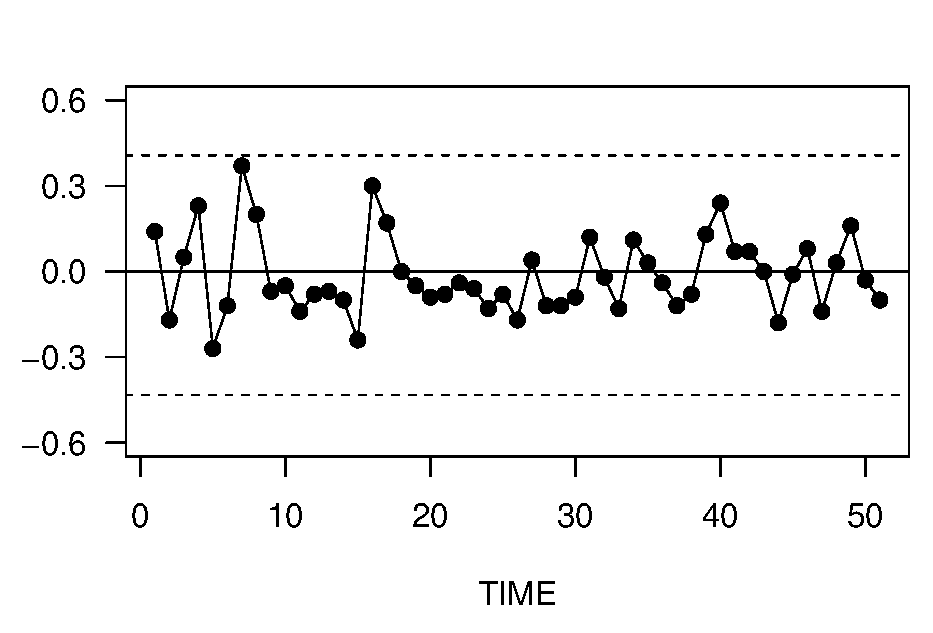
\includegraphics[width=.8\textwidth]
        {Chapter8AutoReg/InfBondControl.eps}
    \caption{\label{F8:InfBondControl} \small Control
Chart of Residuals from an ${\small AR}${\small (1) Fit of the
Inflation Index Series. The dashed lines mark the upper and lower control limits which are
the mean plus and minus three standard deviations.}}
  \end{center}
\end{figure}

\bigskip

\begin{table}[h]
\caption{\label{T8:InfBondResidAuto} Residual Autocorrelations from
the $AR$(1) model}
\begin{center}
\begin{tabular}{c|ccccc}
\hline
Lag $k$ & 1 & 2 & 3 & 4 & 5 \\
Residual Autocorrelation $r_k$ & 0.09 & -0.33 & 0.07 & 0.02 & -0.17 \\
\hline
\end{tabular}\end{center}\end{table}

\linejed

\newpage

\section{Smoothing and Prediction}\label{S8:AR1Smooth}

Having identified, fit, and checked the identification of the model, we now
proceed to basic inference. Recall that by inference we mean the process of
using the data set to make statements about the nature of the world. To make
statements about the series, analysts often examine the values fitted under
the model, called the \emph{smoothed series}. The smoothed series is the
estimated expected value of the series given the past. For the $AR$(1)
model, the smoothed series is%
\begin{equation*}
\widehat{y}_t=b_0+b_1y_{t-1}.
\end{equation*}\index{time series terms and concepts!smoothed series}

In Figure \ref{F8:InfBondSmooth}, an open circle represents the
actual Inflation Bond Index and an opaque circle represents the
corresponding smoothed series. Because the smoothed series is the
actual series with the estimated noise component removed, the
smoothed series is sometimes interpreted to represent the ``real''
value of the series.

\begin{figure}[htp]
  \begin{center}
    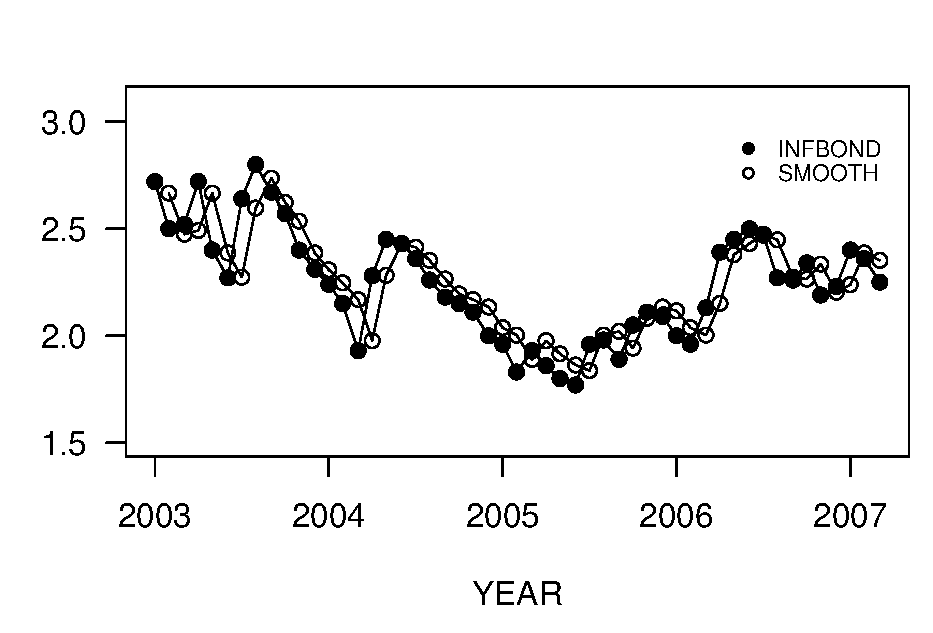
\includegraphics[width=.8\textwidth]
        {Chapter8AutoReg/InfBondSmooth.eps}
    \caption{\label{F8:InfBondSmooth} \small Inflation Bond Index with a Smoothed Series Superimposed. The
index is given by the open plotting symbols, the smoothed series is
represented by the opaque symbols.}
  \end{center}
\end{figure}

Typically, the most important application of time series modeling is
the forecasting of future values of the series. From equation
(\ref{E8:AR1}), the immediate future value of the series is $y_{T+1}
= \beta_0 + \beta_1 y_T + \varepsilon_{T+1}$. Because the series
\{$\varepsilon_t$\} is random, a natural forecast of
$\varepsilon_{T+1}$ is its mean, zero. Thus, if the estimates $b_0$
and $b_1$ are close to the true parameters $\beta_0$ and $\beta_1$,
then a desirable estimate of the series at time $T+1$ is
$\widehat{y}_{T+1} = b_0 + b_1 y_T$. Similarly, one can recursively
compute an estimate for the series $k$ time points in the future,
$y_{T+k}$. \bigskip

\boxedjed \textbf{Definition.} \ The $k$-step ahead forecast of
$y_{T+k}$ for an $AR$ (1) model is recursively determined by
\begin{equation}\label{E8:ChainRule}
\widehat{y}_{T+k} = b_0 + b_1 \widehat{y}_{T+k-1}.
\end{equation}
This is sometimes known as the \emph{chain rule of forecasting}.
\index{time series terms and concepts!chain rule of forecasting}

\end{boxedminipage}
\bigskip

To get an idea of the error in using $\widehat{y}_{T+1}$ to predict
$y_{T+1}$, assume for the moment that the error in using $b_0$ and
$b_1$ to estimate $\beta_0$ and $\beta_1$ is negligible. With this
assumption, the forecast error is
\begin{equation*}
y_{T+1}-\widehat{y}_{T+1} = \beta_0 + \beta_1 y_t +
\varepsilon_{T+1} - \left( b_0 + b_1 y_t\right) \approx
\varepsilon_{T+1}.
\end{equation*}
Thus, the variance of this forecast error is approximately
$\sigma^2$. Similarly, it can be shown that the approximate variance
of the forecast error $y_{T+k}-\widehat{y}_{T+k}$ is $\sigma^2(1 +
\beta_1^2 \ldots + \beta_1^{2(k-1)})$. From this variance
calculation and the approximate normality, we have the following
prediction interval.

\bigskip


\boxedjed

\textbf{Definition.} \ The $k$-step ahead forecast interval of
$y_{T+k}$ for an $AR$(1) model is
\begin{equation*}
\widehat{y}_{T+k} \pm (t-value)~s \sqrt{1 + b_1^2+ \ldots +
b_1^{2(k-1)}}.
\end{equation*}
Here, the $t$-value is a percentile from the $t$-curve using $df=T-3$
degrees of freedom. The percentile is 1 - (prediction level)/2.


\end{boxedminipage}
\bigskip

For example, for 95\% prediction intervals, we would have $t$-value $\approx
$ 2. Thus, one- and two-step 95\% prediction intervals are:

\begin{center}
one-step:$\qquad \widehat{y}_{T+1}\pm \ 2s$

two-step:$\qquad \widehat{y}_{T+2}\pm \ 2s(1+b_1^2)^{1/2}.$
\end{center}

Figure \ref{F8:InfBondForInt} illustrates forecasts of the inflation
bond index. The forecast intervals widen as the number of steps into
the future increases; this reflects our increasing uncertainty as we
forecast further into the future.

\begin{figure}[htp]
  \begin{center}
   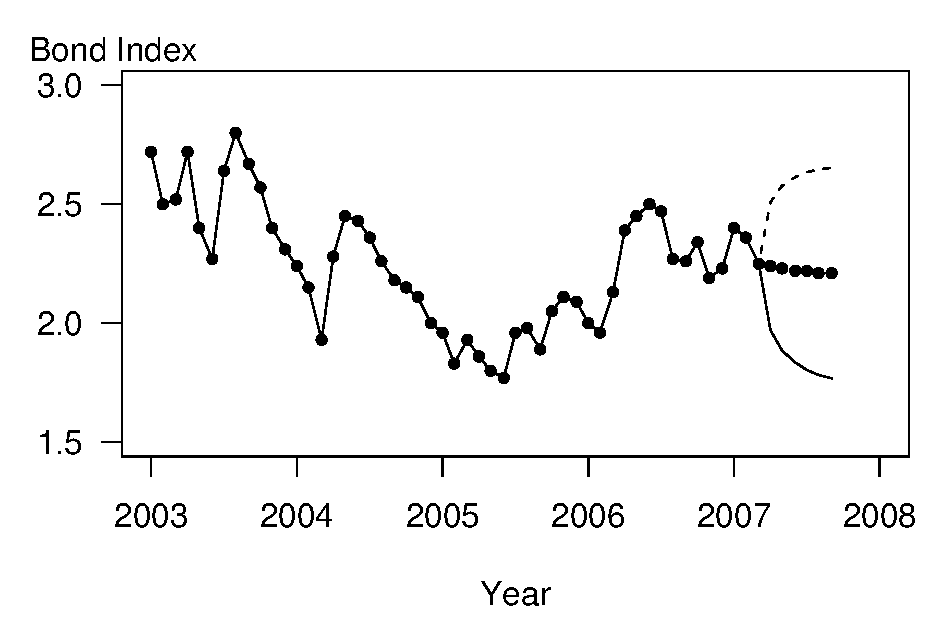
\includegraphics[width=.8\textwidth]{Chapter8AutoReg/InfBondForInt.eps}
    \caption{\label{F8:InfBondForInt} \small Forecast Intervals for the Inflation Bond Series.}
  \end{center}
\end{figure}


\section{Box-Jenkins Modeling and Forecasting}\label{S8:BoxJenkins}

Sections \ref{S8:Autocorrs} through \ref{S8:AR1Smooth} introduced
the $AR(1)$ model, including model properties, identification
methods and forecasting. We now introduce a broader class of models
known as \emph{autoregressive integrated moving average (ARIMA)
models}, due to George Box and Gwilym Jenkins, see Box, Jenkins and
Reinsel (1994).\index{time series models!autoregressive integrated
moving average ($ARIMA$) model}

\subsection{Models}

\subsubsection*{$AR(p)$ Models}\index{time series models!autoregressive model of order $p$, $AR$($p$)}


The autoregressive model of order one allows us to relate the
current behavior of an observation directly to its immediate past
value. Moreover, in some applications, there are also important
effects of observations that are more distant in the past than
simply the immediate preceding observation. To quantify this, we
have already introduced the lag $k$ autocorrelation $\rho_k$ that
captures the linear relationship between $y_t$ and $y_{t-k}$. To
incorporate this feature into a forecasting framework, we have the
\emph{autoregressive model of order p}, denoted by $AR(p).$ The
model equation is
\begin{equation} \label{E8:ARp}
y_t = \beta_0 + \beta_1 y_{t-1} + \ldots + \beta_p y_{t-p} +
\varepsilon_t, \text{ \ \ \ \ \ \ \ \ }t=p+1,\ldots ,T,
\end{equation}
where \{$\varepsilon_t$\} is a white noise process such that
$\mathrm{Cov}(\varepsilon_{t+k}, y_t)=0$ for $k>0$ and $\beta_0$,
$\beta_1,\ldots,\beta_p$ are unknown parameters.

As a convention, when data analysts specify an \textit{AR}($p$)
model, they include not only $y_{t-p}$ as a predictor variable, but
also the intervening lags, $y_{t-1}, \ldots, y_{t-p+1}$. The
exceptions to this convention are the seasonal autoregressive
models, that will be introduced in Section 9.4. Also by convention,
the $AR(p)$ is a model of a stationary, stochastic process. Thus,
certain restrictions on the parameters $\beta_1, \ldots, \beta_p$
are necessary to ensure (weak) stationarity. These restrictions are
developed in the following subsection.

\subsubsection*{Backshift Notation}
\index{time series terms and concepts!backshift operator
B}\index{symbols!B , backshift operator}

The \emph{backshift, or backwards-shift, operator} $\mathrm{B}$ is
defined by $\mathrm{B}y_t$ = $y_{t-1}$. The notation
$\mathrm{B}^{k}$ means apply the operator $k$ times, that is,
\begin{equation*}
\mathrm{B}^{k}~y_t = \mathrm{BB \cdots B~} y_t = \mathrm{B}
^{k-1}~y_{t-1} = \cdots = y_{t-k}.
\end{equation*}%
This operator is linear in the sense that $\mathrm{B} (a_1 y_t + a_2
y_{t-1}) = a_1 y_{t-1} + a_2 y_{t-2}$, where $a_1$ and $a_2$ are
constants. Thus, we can express the $AR(p)$ model as
\begin{eqnarray*}
\beta_0 + \varepsilon_t &=& y_t - \left( \beta_1 y_{t-1} + \ldots +
\beta_p y_{t-p}\right)  \\
&=& \left(1-\beta_1 \mathrm{B} - \ldots - \beta_p
\mathrm{B}^{p}\right) y_t = \Phi \left( \mathrm{B}\right) y_t.
\end{eqnarray*}
If $x$ is a scalar, then $\Phi \left( x\right) = 1 - \beta_1 x -
\ldots - \beta_p x^p$ is a $p$th order polynomial in $x$. Thus,
there exist $p$ roots of the equation $\Phi \left( x\right) =0$.
These roots, say, $g_1,..,g_p$ , may or may not be complex numbers.
It can be shown, see Box, Jenkins and Reinsel (1994), that for
stationarity, all roots lie strictly outside the unit circle. To
illustrate, for $p=1$, we have $\Phi \left( x\right) = 1 - \beta_1
x$. The root of this equation is $g_1 = \beta_1^{-1}$. Thus, we
require $|g_1|>1$, or $|\beta_1|<1$, for stationarity.

\subsubsection*{$MA(q)$ Models}\index{time series models!moving average model of order $q$, $MA$($q$)}

One interpretation of the model $y_t=\beta_0+\varepsilon_t$ is that
the disturbance $\varepsilon_t$\ perturbs the measure of the
\textquotedblleft true,\textquotedblright\ expected value of $y_t.$
Similarly, we can consider the model $y_t=\beta_0 + \varepsilon
_t-\theta_1\varepsilon_{t-1}$, where $\theta_1 \varepsilon_{t-1}$ is
the perturbation from the previous time period. Extending this line
of thought, we introduce the \emph{moving average model of order q},
denoted by
$MA(q)$. The model equation is%
\begin{equation}\label{E8:MAq}
y_t = \beta_0 + \varepsilon_t - \theta_1 \varepsilon_{t-1} - \ldots
- \theta_q \varepsilon_{t-q},
\end{equation}
where the process \{$\varepsilon_t$\} is a white noise process such
that $\mathrm{Cov}(\varepsilon_{t+k}, y_t)=0$ for $k>0$ and
$\beta_0$, $\theta_1, \ldots, \theta_q$ are unknown parameters.

With equation (\ref{E8:MAq}) it is easy to see that $\mathrm{Cov}
(y_{t+k},y_t)=0$ for $k>q$. Thus, $\rho_k =0$ for $k>q$. Unlike the
$AR(p)$ model, the $MA(q)$ process is stationary for any finite
values of the parameters $\beta_0$, $\theta_1, \ldots, \theta_q$. It
is convenient to write the $MA(q)$ using backshift notation, as
follows:
\begin{equation*}
y_t - \beta_0 = \left( 1-\theta_1\mathrm{B} - \ldots - \theta_q
\mathrm{B}^q\right) \varepsilon_t = \Theta \left( \mathrm{B}\right)
\varepsilon_t.
\end{equation*}
As with $\Phi \left( x\right) $, if $x$ is a scalar, then $\Theta
\left( x\right) = 1 - \theta_1 x - \ldots - \theta_q x^q$ is a $q$th
order polynomial in $x$. It is unfortunate that the phrase ``moving
average'' is used for the model defined by equation (\ref{E8:MAq})
and the estimate defined in Section 9.2. We will attempt to clarify
the usage as it arises.

\subsubsection*{$ARMA$ and $ARIMA$ Models}\index{time series models!autoregressive moving average ($ARMA$) model}

Combining the $AR(p)$ and the $MA(q)$ models yields the
\emph{autoregressive moving average model} of order $p$ and $q$, or
$ARMA(p,q)$,
\begin{equation}\label{E8:ARMApq}
y_t - \beta_1 y_{t-1} - \ldots - \beta_p y_{t-p} = \beta_0 +
\varepsilon _t - \theta_1 \varepsilon_{t-1} - \ldots - \theta_q
\varepsilon_{t-q},
\end{equation}
which can be represented as
\begin{equation}
\Phi \left( \mathrm{B}\right) y_t = \beta_0 + \Theta \left(
\mathrm{B} \right) \varepsilon_t.
\end{equation}

In many applications, the data requires differencing to exhibit
stationarity. We assume that the data are differenced $d$ times to
yield
\begin{equation}\label{E8:Diffd}
w_t = \left( 1-\mathrm{B}\right)^d y_t = \left( 1-\mathrm{B}\right)
^{d-1}\left( y_t-y_{t-1}\right) = \left( 1-\mathrm{B}\right)
^{d-2}\left( y_t-y_{t-1}-\left( y_{t-1}-y_{t-2}\right) \right) =
\ldots
\end{equation}
In practice, $d$ is typically zero, one or two. With this, the
\emph{autoregressive integrated moving average model} of order
$(p,d,q)$, denoted by $ARIMA(p,d,q)$, is\index{time series
models!autoregressive integrated moving average ($ARIMA$) model}
\begin{equation}
\Phi \left( \mathrm{B}\right) w_t = \beta_0+\Theta \left( \mathrm{B}
\right) \varepsilon_t.
\end{equation}
Often, $\beta_0$ is zero for $d>0$.

Several procedures are available for estimating model parameters including
maximum likelihood estimation, and conditional and unconditional least
squares estimation. In most cases, these procedures require iterative
fitting procedures. See Abraham and Ledolter (1983) for further information.

\linejed

\index{examples!Lee-Carter mortality rate forecasts}

\textbf{Example: Forecasting Mortality Rates}\ecaptionjed{Lee-Carter
Mortality Rate Forecasts}. To quantify values in life insurance and
annuities, actuaries need forecasts of age-specific mortality rates.
Since its publication, the method proposed by Lee and Carter (1992)
has proved to be a popular method to forecast mortality. For
example, Li and Chan (2007) used these methods to produce forecasts
of 1921-2000 Canadian population rates and 1900-2000 U.S. rates.
They showed how to modify the basic methodology to incorporate
atypical events including wars and pandemic events such as influenza
and pneumonia.

The Lee-Carter method is usually based on central death rates at age
$x$ at time $t$, denoted by $m_{x,t}$. The model equation is
\begin{equation}\label{E8:LeeCarter}
m_{x,t} = \alpha_x + \beta_x \kappa_t + \varepsilon_{x,t} .
\end{equation}
Here, the intercept ($\alpha_x$) and slope ($\beta_x$) depend only
on age $x$, not on time $t$. The parameter $\kappa_t$ captures the
important time effects (except for those in the disturbance term
$\varepsilon_{x,t}$).

At first glance, the Lee-Carter model appears to be a linear
regression with one explanatory variable. However, the term
$\kappa_t$ is not observed and so different techniques are required
for model estimation. Different algorithms are available, including
the singular value decomposition proposed by Lee and Carter, the
principal components approach and a Poisson regression model; see Li
and Chan (2007) for references.\index{principal components}

The time-varying term $\kappa_t$ is typically represented using an
$ARIMA$ model. Li and Chan found that a random walk (with
adjustments for unusual events) was a suitable model for Canadian
and U.S. rates (with different coefficients), reinforcing the
findings of Lee and Carter.



\linejed \bigskip



\subsection{Forecasting}

\subsubsection*{Optimal Point Forecasts}

Similar to forecasts that were introduced in Section
\ref{S8:AR1Smooth}, it is common to provide forecasts that are
estimates of conditional expectations of the predictive
distribution. Specifically, assume we have available a realization
of \{$y_1, y_2, \ldots, y_T$\} and would like to forecast $y_{T+l}$,
the value of the series ``$l$'' lead time units in the future. If
the parameters of the process were known, then we would use
$\mathrm{E}(y_{T+l}|y_T,y_{T-1},y_{T-2},\ldots)$, that is, the
conditional expectation of $y_{T+l}$ given the value of the series
up to and including time $T$. We use the notation $\mathrm{E}_T$ for
this conditional expectation.

To illustrate, taking $t=T+l$ and applying $\mathrm{E}_T$\ to both
sides of equation (\ref{E8:ARMApq}) yields
\begin{equation}\label{E8:ChainRuleForecasting}
y_T(l) - \beta_1 y_T(l-1) - \ldots - \beta_p y_T(l-p) = \beta_0 +
\mathrm{E}_T\left( \varepsilon_{T+l} - \theta_1 \varepsilon_{T+l-1}
- \ldots - \theta _q \varepsilon_{T+l-q}\right) ,
\end{equation}
using the notation $y_T(k) = \mathrm{E}_T\left( y_{T+k}\right) $.
For $k \leq 0$, $\mathrm{E}_T\left( y_{T+k}\right) =y_{T+k}$, as the
value of $y_{T+k}$\ is known at time $T$. Further,
$\mathrm{E}_T\left( \varepsilon_{T+k}\right) =0$ for $k>0$ as
disturbance terms in the future are assumed to be uncorrelated with
current and past values of the series. Thus, equation
(\ref{E8:ChainRuleForecasting}) provides the basis of the
\emph{chain rule of forecasting}, where we recursively provide
forecasts at lead time $l$ based on prior forecasts and realizations
of the series. To implement equation
(\ref{E8:ChainRuleForecasting}), we substitute estimates for
parameters and residuals for disturbance terms.\index{time series
terms and concepts!chain rule of forecasting}

\textbf{Special Case - MA(1) Model}. We have already seen the
forecasting chain rule for the $AR(1)$ model in Section
\ref{S8:AR1Smooth}. For the $MA(1)$ model, note that for $l\geq 2$,
we have $y_T(l)=\mathrm{E}_T\left( y_{T+l}\right)
=\mathrm{E}_T\left(
\beta_0+\varepsilon_{T+l}-\theta_1\varepsilon_{T+l-1}\right)
=\beta_0$, because $\varepsilon_{T+l}$\ and $\varepsilon _{T+l-1}$\
are in the future at time $T$. For $l=1$, we have $y_T(1)=
\mathrm{E}_T\left( \beta_0+\varepsilon_{T+1}-\theta
_1\varepsilon_T\right) =\beta_0-\theta_1\mathrm{E}_T\left(
\varepsilon_T\right) $. Typically, one would estimate the term
$\mathrm{E}_T\left( \varepsilon_T\right) $\ using the residual at
time $T$.


\subsubsection*{$\protect\psi $-Coefficient Representation}

Any $ARIMA(p,d,q)$ model can be expressed as%
\begin{equation*}
y_t=\beta_0^{\ast }+\varepsilon_t+\psi_1 \varepsilon_{t-1}+\psi
_2\varepsilon_{t-2}+\ldots=\beta_0^{\ast }+\sum_{k=0}^{\infty }\psi
_{k}\varepsilon_{t-k},
\end{equation*}%
called the $\psi $\emph{-coefficient representation}. That is, the
current value of a process can be expressed as a constant plus a
linear combination of the current and previous disturbances. Values
of \{$\psi_{k}$\} depend on the linear parameters of the $ARIMA$
process and can be determined via straightforward recursive
substitution. To illustrate, for the $AR(1)$ model, we have
\begin{eqnarray*}
y_t &=&\beta_0+\varepsilon_t+\beta_1y_{t-1}=\beta_0+\varepsilon
_t+\beta_1\left( \beta_0+\varepsilon
_{t-1}+\beta_1y_{t-2}\right) =\ldots \\
&=&\frac{\beta_0}{1-\beta_1}+\varepsilon_t+\beta_1\varepsilon
_{t-1}+\beta_1^2\varepsilon_{t-2}+\ldots=\frac{\beta_0}{1-\beta_1}%
+\sum_{k=0}^{\infty }\beta_1^{k}\varepsilon_{t-k}.
\end{eqnarray*}%
That is, $\psi_{k}=\beta_1^{k}$.\index{time series terms and
concepts!$\psi $-coefficient representation}

\subsubsection*{Forecast Interval}

Using the $\psi $-coefficient representation, we can express the
conditional expectation of $y_{T+l}$ as
\begin{equation*}
\mathrm{E}_T\left( y_{T+l}\right) =\beta_0^{\ast
}+\sum_{k=0}^{\infty }\psi_{k}\mathrm{E}_T\left( \varepsilon
_{T+l-k}\right) =\beta_0^{\ast }+\sum_{k=l}^{\infty }\psi
_{k}\mathrm{E}_T\left( \varepsilon_{T+l-k}\right) .
\end{equation*}
This is because, at time $T$, the errors $\varepsilon_T,\varepsilon
_{T-1},\ldots$, have been determined by the realization of the
process. However, the errors
$\varepsilon_{T+1},\ldots,\varepsilon_{T+l}$ have not been realized
and hence have conditional expectation zero. Thus, the $l$-step
forecast error is
\begin{equation*}
y_{T+l}-\mathrm{E}_T\left( y_{T+l}\right) =\beta_0^{\ast
}+\sum_{k=0}^{\infty }\psi_{k}\varepsilon_{T+l-k}-\left(
\beta_0^{\ast }+\sum_{k=l}^{\infty }\psi_{k}\mathrm{E}_T\left(
\varepsilon _{T+l-k}\right) \right)
=\sum_{k=0}^{l-1}\psi_{k}\varepsilon _{T+l-k}.
\end{equation*}

We focus on the variability of the forecasts errors. That is,
straightforward calculations yield $\mathrm{Var}\left(
y_{T+l}-\mathrm{E}_T \left( y_{T+l}\right) \right)
=\sigma^2\sum_{k=1}^{l-1}\psi_{k}^2$. Thus, assuming normality of
the errors, a $100(1-\alpha) \%$ forecast interval for $y_{T+l}$ is
\begin{equation*}
\widehat{y}_{T+l} \pm (t-value) s \sqrt{\sum_{k=0}^{l-1}
\widehat{\psi}_k^2} .
\end{equation*}
where $t$-value is the $(1-\alpha /2)^{th}$ percentile from a
$t$-distribution with $df=T-(number~of~linear~parameters)$. If $y_t$
is an $ARIMA(p,d,q)$ process, then $\psi_{k}$ is a function of
$\beta_1,\ldots,\beta_p,\theta_1,\ldots,\theta_q$ and the number of
linear parameters is $1+p+q$.

\section{Application: Hong Kong Exchange Rates}\index{datasets!Hong Kong exchange rates}\empexjed{HKExchange}

Section 7.2 introduced the Hong Kong Exchange Rate series, based on
$T=502$ daily observations for the period April 1, 2005 through Mary
31, 2007. A quadratic trend was fit to the model that produced an
$R^2=86.2\%$ with a residual standard deviation of $s=0.0068$. We
now show how to improve on this fit using $ARIMA$ modeling.

To begin, Figure \ref{F8:HKResids} shows a time series plot of
residuals from the quadratic trend time model. This plot displays a
meandering pattern, suggesting that there is information in the
residuals that can be exploited.

\begin{figure}[htp]
  \begin{center}
   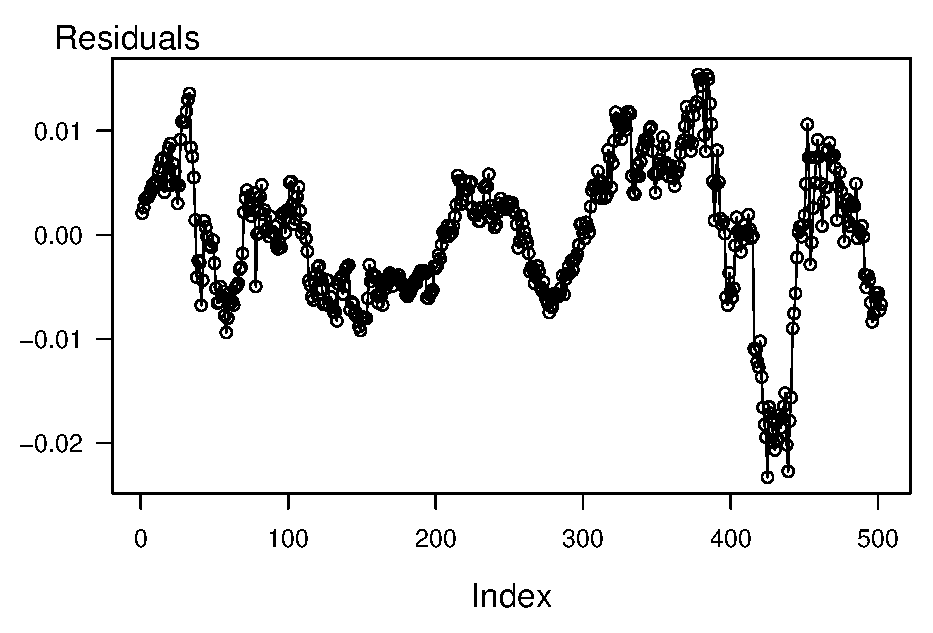
\includegraphics[width=.8\textwidth]{Chapter8AutoReg/HKResids.eps}
   \caption{\label{F8:HKResids} \small Residuals from a Quadratic Trend in Time
Model of the Hong Kong Exchange Rates.}
  \end{center}
\end{figure}



Further evidence of these patterns is in the table of
autocorrelations in Table \ref{T8:HKRatesAuto}. Here, we see large
residual autocorrelations that do not decrease quickly as the lag
$k$ increases. A similar pattern is also evident for the original
series, EXHKUS. This confirms the nonstationarity that we observed
in Section 7.2.

As an alternative transform, we differenced the series, producing
DIFFHKUS. This differenced series has a standard deviation of
$s_{DIFF}=0.0020$, suggesting that it is more stable than the
original series or the residuals from the quadratic trend in time
model. Table \ref{T8:HKRatesAuto} presents the autocorrelations from
the differenced series, indicating mild patterns. However, these
autocorrelations are still significantly different from zero. For
$T=501$ differences, we may use as an approximate standard error for
autocorrelations $1/\sqrt{501}\approx 0.0447.$ With this, we see
that the lag 2 autocorrelation is $0.151/0.0447\approx 3.38$
standard errors below zero, which is statistically significant. This
suggests introducing another model to take advantage of the
information in the time series patterns.

\bigskip

\begin{table}[h]
\scalefont{0.8}
 \caption{\label{T8:HKRatesAuto} Autocorrelations of
Hong Kong Exchange Rates}
\begin{center}
\begin{tabular}{l|cccccccccc}
\hline
Lag & 1 & 2 & 3 & 4 & 5 & 6 & 7 & 8 & 9 & 10 \\
Residuals from the & 0.958 & 0.910 & 0.876 & 0.847 & 0.819 & 0.783 & 0.748 &
0.711 & 0.677 & 0.636 \\
\ \ Quadratic Model &  &  &  &  &  &  &  &  &  &  \\
EXHKUS  & 0.988 & 0.975 & 0.963 & 0.952 & 0.942 & 0.930 & 0.919 &
0.907 & 0.895
& 0.882 \\
\ \ (Original Series) &  &  &  &  &  &  &  &  &  &  \\
DIFFHKUS & 0.078 & -0.151 & -0.038 & -0.001 & 0.095 & -0.005 & 0.051
& -0.012 & 0.084 & -0.001 \\ \hline
\end{tabular}\end{center}

\scalefont{1.25}\end{table}

\subsubsection*{Model Selection and Partial
Autocorrelations}\index{correlation coefficients!partial
autocorrelation}

\marginparjed{For stationary autoregressive models, $|\rho_k|$
becomes small as the lag $k$ increases.}

For all stationary autoregressive models, it can be shown that the
absolute values of the autocorrelations become small as the lag $k$
increases. In the case that the autocorrelations decrease
approximately like a geometric series, an \textit{AR}(1) model may
be identified. Unfortunately, for other types of autoregressive
series, the rules of thumb for identifying the series from the
autocorrelations become more cloudy. One device that is useful for
identifying the order of an autoregressive series is the
\emph{partial autocorrelation function}.

Just like autocorrelations, we now define a \emph{partial
autocorrelation} at a specific lag $k$. Consider the model equation
\begin{equation*}
y_t=\beta_{0,k}+\beta_{1,k} y_{t-1}+\ldots+\beta_{k,k} y_{t-k} +
\varepsilon_t.
\end{equation*}
Here, \{$\varepsilon_t$\} is a stationary error that may or may not
be a white noise process. The second subscript on the $\beta$'s,
``$,k$'', is there to remind us that the value of each $\beta $ may
change when the order of the model, $k$, changes. With this model
specification, we can interpret $\beta_{k,k}$ as the correlation
between $y_t$ and $y_{t-k}$ after the effects of the intervening
variables, $y_{t-1},\ldots,y_{t-k+1}$, have been removed. This is
the same idea as the partial correlation coefficient, introduced in
Section 4.4. Estimates of partial correlation coefficients,
$b_{k,k}$, can then be calculated using conditional least squares or
other techniques. As with other correlations, we may use
$1/\sqrt{T}$ as an approximate standard error for detecting
significant differences from zero.

\marginparjed{A lag k partial autocorrelation is the correlation
between $y_t$ and $y_{t-k}$, controlling for the effects of the
intervening variables, $y_{t-1},\ldots,y_{t-k+1}$.}

Partial autocorrelations are used in model identification in the following
way. First calculate the first several estimates, $b_{1,1},b_{2,2},b_{3,3}$,
and so on. Then, choose the order of the autoregressive model to be the
largest $k$ so that the estimate $b_{k,k}$ is significantly different from
zero.

To see how this applies in the Hong Kong Exchange Rate example,
recall that the approximate standard error for correlations is
$1/\sqrt{501}\approx 0.0447$. Table \ref{T8:PartialAuto} provides
the first ten partial autocorrelations for the rates and for their
differences. Using twice the standard error as our cut-off rule, we
see that the second partial autocorrelation of the differences
exceeds $2\times 0.0447=0.0894$ in absolute value. This would
suggest using an $AR(2)$ as a tentative first model choice.
Alternatively, the reader may wish to argue that because the fifth
and ninth partial autocorrelations are also statistically
significant, suggesting a more complex $AR(5)$ or $AR(9)$ would be
more appropriate. The philosophy is to ``use the simplest model
possible, but no simpler.'' We prefer to employ simpler models and
thus fit these first and then test to see whether or not they
capture the important aspects of the data.

\marginparjed{Another way of identifying a series as nonstationary
is to examine the partial autocorrelation function and look for a
large lag one partial autocorrelation.}

Finally, you may be interested to see what happens to partial
autocorrelations calculated on a non-stationary series. Table
\ref{T8:PartialAuto} provides partial autocorrelations for the
original series (EXHKUS). Note how large the first partial
autocorrelation is. That is, yet another way of identifying a series
as nonstationary is to examine the partial autocorrelation function
and look for a large lag one partial autocorrelation.


\begin{table}[h]
\scalefont{0.9} \caption{\label{T8:PartialAuto} Partial
Autocorrelations of EXHKUS and DIFFHKUS}
\begin{tabular}{c|cccccccccc}
\hline
Lag & 1 & 2 & 3 & 4 & 5 & 6 & 7 & 8 & 9 & 10 \\
EXHKUS & 0.988 & -0.034 & 0.051 & 0.019 & -0.001 & -0.023 & 0.010 &
-0.047 &
-0.013 & -0.049 \\
DIFFHKUS & 0.078 & -0.158 & -0.013 & -0.021 & 0.092 & -0.026 & 0.085
& -0.027 & 0.117 & -0.036 \\ \hline
\end{tabular}\scalefont{1.1111}
\end{table}


\subsubsection*{Residual Checking}

Having identified and fit a model, residual checking is still an important
part of determining a model's validity. For the $ARMA(p,q)$ model, we
compute fitted values as

\begin{equation}\label{E8:ARMAFittedValues}
\widehat{y}_t = b_0 + b_1 y_{t-1} + \ldots + b_p y_{t-p} -
\widehat{\theta}_1 e_{t-1}- \ldots - \widehat{\theta }_q e_{t-q}.
\end{equation}
Here, $\widehat{\theta}_1, \ldots, \widehat{\theta}_q$ are estimates
of $\theta_1,\ldots, \theta_q$. The residuals may be computed in the
usual fashion, that is, as $e_t=y_t-\widehat{y}_t$. Without further
approximations, note that the initial residuals are missing because
fitted values before time $t=\max (p,q)$ can not be calculated using
equation (\ref{E8:ARMAFittedValues}). To check for patterns, use the
devices described in Section \ref{S8:Estimation}, such as the
control chart to check for stationarity and the autocorrelation
function to check for lagged variable relationships.

\subsubsection*{Residual Autocorrelation}

Residuals from the fitted model should resemble white noise and
hence, display few discernible patterns. In particular, we expect
$r_k(e)$, the lag $k$ autocorrelation of residuals, to be
approximately zero. To assess this, we have that $se\left( r_k(e)
\right) \approx 1/\sqrt{T}$. More precisely, MacLeod (1977, 1978)
has given approximations for a broad class of $ARMA$ models. It
turns out that the $1/\sqrt{T}$ can be improved for small values of
$k$. (These improved values can be seen in the output of most
statistical packages.) The improvement depends on the model that is
being fit. To illustrate, suppose that an $AR(1)$ model with
autoregressive parameter $\beta_1$ is fit to the data. Then, the
approximate standard error of the lag one residual autocorrelation
is $|\beta_1|/\sqrt{T}$ . This standard error can be much smaller
than $1/\sqrt{T}$, depending on the value of $\beta_1$.

\subsubsection*{Testing Several Lags}

To test whether there is significant residual autocorrelation at a
specific lag $k$, we use $r_k(e) /se\left( r_k(e) \right)$. Further,
to check whether residuals resemble a white noise process, we might
test whether $r_k(e)$ is close to zero for several values of $k$. To
test whether the first $K$ residual autocorrelation are zero, use
the Box and Pierce (1970) chi-square statistic\index{time series
statistics!Box-Pierce chi-square}\index{distributions!chi-square}
\begin{equation*}
Q_{BP} = T \sum_{k=1}^{K} r_k \left( e \right)^2.
\end{equation*}
Here, $K$ is an integer that is user-specified. If there is no real
autocorrelation, then we expect $Q_{BP}$ to be small; more
precisely, Box and Pierce showed that $Q_{BP}$ follows an
approximate $\chi^2$ distribution with
$df=K-(number~of~linear~parameters)$. For an $ARMA(p,q)$ model, the
number of linear parameters is $1+p+q.$ Another widely used
statistic is
\begin{equation*}
Q_{LB}=T(T+2)\sum_{k=1}^{K}\frac{r_k \left( e\right)^2}{T-k}.
\end{equation*}
\marginparjed{Appendix A3.2 provides additional details about the
chi-square distribution, including a graph and percentiles.}

\noindent due to Ljung and Box (1978). This statistic performs
better in small samples than the $BP$ statistic. Under the
hypothesis of no residual autocorrelation, $Q_{LB}$ follows the same
$\chi^2$ distribution as $Q_{BP}$. Thus, for each statistic, we
reject $H_{0}$: No Residual Autocorrelation if the statistic exceeds
$chi$-value, a $1-\alpha$ percentile from a $\chi^2$ distribution. A
convenient rule of thumb is to use $chi$-value = 1.5
$df.$\index{time series statistics!Box-Ljung chi-square}

\linejed\index{datasets!Hong Kong exchange rates}

\textbf{Example: Hong Kong Exchange Rate - Continued.} Two models
were fit, the $ARIMA(2,1,0)$ and the $ARIMA(0,1,2)$; these are the
$AR(2)$ and $MA(2)$ models after taking differences. Using \{$y_t$\}
for the differences, the estimated $AR(2)$ model is:
\begin{equation*}
\begin{tabular}{clllrllll}
$\widehat{y}_t$ & $=$ & $0.0000317$ & $+$ & $0.0900$ & $y_{t-1}$ & $-$ & $%
0.158$ & $y_{t-2}$ \\
\multicolumn{1}{l}{\small $t$-statistic} &  &
\multicolumn{1}{c}{\small [0.37]} &  & \multicolumn{1}{c}{\small
[2.03]} &
 & & \multicolumn{1}{c}{\small
[-3.57]} &
\end{tabular}
\end{equation*}
with a residual standard error of $s=0.00193.$ The estimated $MA(2)$
is:
\begin{equation*}
\begin{tabular}{clllrllll}
$\widehat{y}_t$ & $=$ & $0.0000297$ & $-$ & $0.0920$ & $e_{t-1}$ & $+$ & $%
0.162$ & $e_{t-2}$ \\
\multicolumn{1}{l}{\small $t$-statistic} &  &
\multicolumn{1}{c}{\small [0.37]} & & \multicolumn{1}{c}{\small
[-2.08]} & &  & \multicolumn{1}{c}{\small [3.66]} &
\end{tabular}
\end{equation*}
with the same residual standard error of $s=0.00193.$ These
statistics indicate that the models are roughly comparable. The
Ljung-Box statistic in Table \ref{T8:HKRatesLB} also indicates a
great deal of similarity for the models.

\bigskip

\begin{table}[h]
\caption{\label{T8:HKRatesLB} Ljung-Box Statistics $Q_{LB}$ for Hong
Kong Exchange Rate Models}
\begin{tabular}{lccccc}
\hline
& \multicolumn{5}{c}{Lag $K$} \\
Model  & 2 & 4 & 6 & 8 & 10 \\  \hline
$AR(2)$ & 0.0050 & 0.5705 & 6.3572 & 10.4746 & 16.3565 \\
$MA(2)$ & 0.0146 & 0.2900 & 6.6661 & 11.3655 & 17.7326 \\ \hline
\end{tabular}
\end{table}

The fitted $MA$(2) and $AR$(2) models are roughly similar. We
present the $AR$(2) model for forecasting only because
autoregressive models are typically easier to interpret. Figure
\ref{F8:HKForecast} summarizes the predictions, calculated for ten
days. Note the widening forecast intervals, typical of forecasts for
nonstationary series.
\begin{figure}[htp]
  \begin{center}
    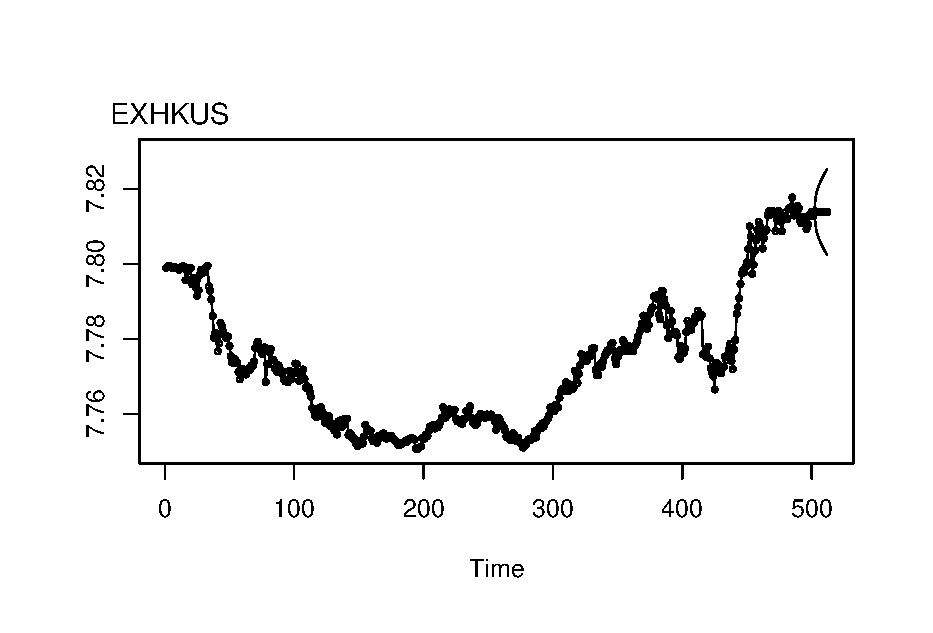
\includegraphics[width=.8\textwidth]{Chapter8AutoReg/F88ARI21Fore.eps}
    \caption{\label{F8:HKForecast} \small Ten Day Forecasts and Forecast Intervals of the Hong Kong Exchange Rates.
    Forecasts are based on the ARIMA(2,1,0) model.}
  \end{center}
\end{figure}

\linejed
\bigskip



\section{Further Reading and References}

The classic book-long introduction to Box-Jenkins time series is
Box, Jenkins and Reinsel (1994).

\bigskip


\textbf{Chapter References}

\begin{multicols}{2}

\scalefont{0.9}

Abraham, Bovas and  Johannes Ledolter (1983). \textit{Statistical
Methods for Forecasting}. John Wiley \& Sons, New York.

Box, George E. P., Gwilym M. Jenkins and Gregory C. Reinsel (1994).
\textit{Time Series Analysis: Forecasting and Control}, Third
Edition, Prentice-Hall, Englewood Cliffs, New Jersey.

Box, George E. P., and D. A. Pierce (1970). Distribution of residual
autocorrelations in autoregressive moving average time series
models. \textit{Journal of the American Statistical Association} 65,
1509-1526.

Chan, Wai-Sum and Siu-Hang Li (2007). The Lee-Carter model for
forecasting mortality, revisited. \textit{North American Actuarial
Journal} 11(1), 68-89.

Lee, Ronald D. and Lawrence R. Carter (1992). Modelling and
forecasting U.S. mortality. \textit{Journal of the American
Statistical Association} 87, 659-671.

Ljung, G. M. and George E. P. Box (1978). On a measure of lack of
fit in time series models. \textit{Biometrika} 65, 297-303.

MacLeod, A. I. (1977). Improved Box-Jenkins estimators.
\textit{Biometrika} 64, 531-534.

MacLeod, A. I. (1978). On the distribution of residual
autocorrelations in Box-Jenkins models. \textit{Journal of the Royal
Statistical Society B} 40, 296-302.

Miller, Robert B. and Dean W. Wichern (1977). \emph{Intermediate
Business Statistics: Analysis of Variance, Regression and Time
Series}. Holt, Rinehart and Winston, New York.

Roberts, Harry V. (1991). \emph{Data Analysis for Managers with
MINITAB}. Scientific Press, South San Francisco, CA.

\scalefont{1.1111}

\end{multicols}

\section{Exercises}

\scalefont{0.90}
\begin{exercises}

\item A mutual fund has provided investment yield rates for five consecutive years as follows:
\begin{center}
\begin{tabular}{lccccc}
  \hline
 Year & 1 & 2 & 3 & 4 & 5 \\
Yield & 0.09 & 0.08 & 0.09 & 0.12 & -0.03 \\
  \hline
\end{tabular}\end{center}

Determine $r_1$ and $r_2$, the lag 1 and lag 2 autocorrelation
coefficients.

\item The \textit{Durbin-Watson} statistic is designed to detect autocorrelation and is defined by:
\begin{equation*}
DW = \frac {\sum_{t=2}^T (y_t - y_{t-1})^2} {\sum_{t=1}^T (y_t -
\bar{y})^2}.
\end{equation*}\index{time series
statistics!Durbin-Watson}


a. Derive the approximate relationship between $DW$ and the lag 1
autocorrelation coefficient $r_1$.

b. Suppose that $r_1 = 0.4$. What is the approximate value of $DW$?



\item Consider the Chapter 2 linear regression model formulas with
$y_{t-1}$ in place of $x_t$, for $t=2, \ldots, T$.

a. Provide an exact expression for $b_1$.

b. Provide an exact expression for $b_0$.

c. Show that $b_0 \approx \bar{y} (1-r_1) $.

\item Begin with the $AR$(1) model as in equation (\ref{E8:AR1}).

a. Take variances of each side of equation (\ref{E8:AR1}) to show
that $\sigma_y^2(1-\beta_1^2) = \sigma^2,$ where $\sigma_y^2 =
\mathrm{Var}~y_t$ and $\sigma^2 = \mathrm{Var}~\varepsilon_t$.

b. Show that $\mathrm{Cov}(y_t,y_{t-1}) = \beta_1 \sigma_y^2.$

c. Show that $\mathrm{Cov}(y_t,y_{t-k}) = \beta_1^k \sigma_y^2.$

d. Use part (c) to establish equation
(\ref{E8:AR1Autocorrelations}).

\item Consider forecasting with the $AR$(1) model.

a. Use the forecasting chain rule in equation (\ref{E8:ChainRule})
to show
\begin{equation*}
y_{T+k}-\widehat{y}_{T+k} \approx \varepsilon_{T+k} + \beta_1
\varepsilon_{T+k-1} + \cdots + \beta_1^{k-1} \varepsilon_{T+1}.
\end{equation*}

b. From part (a), show that the approximate variance of the forecast
error is $\sigma^2 \sum_{l=0}^{k-1} \beta_1^{2l}.$


\index{datasets!Standard and Poor's daily
returns}\empexjed{SP500Daily}
\item These data consist of the 503 daily returns for the calendar
years 2005 and 2006 of the Standard and Poor's (S\&P) value weighted
index. (The data file contains additional years - this exercise uses
only 2005 and 2006 data.) Each year, there are about 250 days on
which the exchange is open and stocks were traded - on weekends and
holidays it is closed. There are several indices to measure the
market's overall performance. The \textit{value weighted index} is
created by assuming that the amount invested in each stock is
proportional to its market capitalization. Here, the market
capitalization is simply the beginning price per share times the
number of outstanding shares. An alternative is the \textit{equally
weighted index}, created by taking a simple average of the closing,
or last, price of stocks that form the S\&P on that trading day.

Financial economic theory states that if the market were predictable, many
investors would attempt to take advantage of these predictions, thus forcing
unpredictability. For example, suppose a statistical model reliably
predicted mutual fund A to increase two-fold over the next 18 months. Then,
the no arbitrage principle in financial economics states that several alert
investors, armed with information from the statistical model, would bid to
buy mutual fund A, thus causing the price to increase because demand is
increasing. These alert investors would continue to purchase until the price
of mutual fund A rose to the point where the return was equivalent to other
investment opportunities in the same risk class. Thus, any advantages
produced by the statistical model would disappear rapidly, thus eliminating
this advantage.

Thus, financial economic theory states that for liquid markets such
as stocks represented through the S\&P index there should be no
detectable patterns, resulting in a white noise process. In
practice, it has been found that cost of buying and selling equities
(called transactions costs) are large enough so as to prevent us
from taking advantage of these slight tendencies in the swings of
the market. This illustrates a point known as \emph{statistically
significant but not practically important}. This is not to suggest
that statistics is not practical (heavens forbid!). Instead,
statistics in and of itself does not explicitly recognize factors,
such as economic, psychological and so on, that may be extremely
important in any given situation. It is up to the analyst to
interpret the statistical analysis in light of these
factors.\bigskip


\begin{figure}[htp]
  \begin{center}
   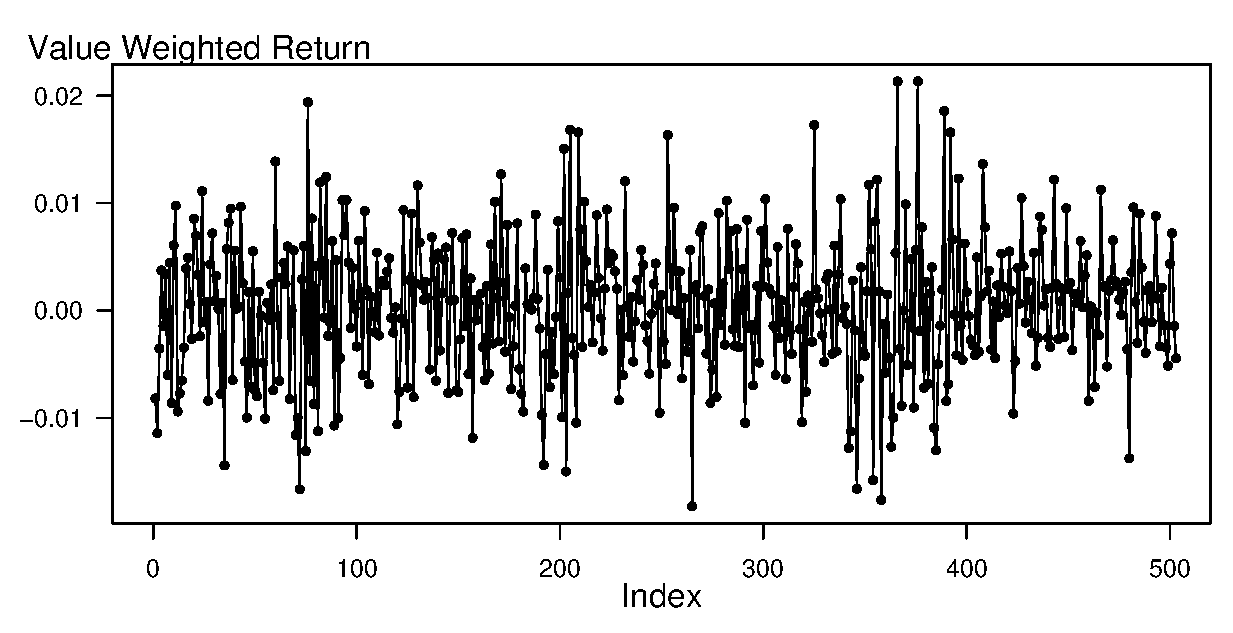
\includegraphics[width=.8\textwidth]{Chapter8AutoReg/ValueWgtReturn.eps}
      \caption{\label{F8:SPValue} \small Time Series Plot of the S \& P Daily Market Return, 2005-2006.}
      \end{center}
\end{figure}


a. The time series plot in Figure \ref{F8:SPValue} gives a
preliminary idea of the characteristics of the sequence. Comment on
the stationarity of the sequence.

b. Calculate summary statistics of the sequence. Suppose that you assume a
white noise model for the the sequence. Compute 1, 2 and 3 step ahead
forecasts for the daily returns for the first three trading days of 2007.

c. Calculate the autocorrelations for the lags 1 through 10. Do you detect
any autocorrelations that are statistically significantly different from
zero?


\end{exercises}
\scalefont{1.1111}

\input{Chapter9Forecasting/Chap9_Forecasting26Apr2009.tex}
%\index{examples|see{data}}
%\index{graphs|see{plots}}\index{multicollinearity|see{collinearity}}

\setcounter{chapter}{9}
\chapter{Longitudinal and Panel Data Models}

{\small \textit{Chapter Preview}. Longitudinal data, also known as
panel data, are composed of a cross-section of subjects that we
observe repeatedly over time. Longitudinal data allow us to study
cross-sectional and dynamic patterns simultaneously; this chapter
describes several techniques for visualizing longitudinal data. Two
types of models are introduced, fixed and random effects models.
This chapter shows how to estimate fixed effects models using
categorical explanatory variables. Estimation for random effects
models is deferred to a later chapter; this chapter describes when
and how to use these models.}

\section{What are Longitudinal and Panel Data?}\label{S10:Intro}

In Chapters 1--6 we studied cross-sectional regression techniques
that allowed us to predict a dependent variable $y$ using
explanatory variables $x$. For many problems, the best predictor is
a value from the preceding period; the times series methods we
studied in Chapters 7--9 use the history of a dependent variable for
prediction. For example, an actuary seeking to predict insurance
claims for a small business will often find that last year's claims
are the best predictor. However, a limitation of time series methods
is that they are based on having available many observations over
time (typically 30 or more). When studying annual claims from a
business, a long time series is rarely available; either businesses
do not have the data or, if they do, it is unreasonable to use the
same stochastic model for today's claims as for those 30 years in
the past. We would like a model that allows us to use information
about company characteristics, explanatory variables such as
industry, number of employees, age and gender composition, and so
forth, as well as \emph{recent} claims history. That is, we need a
model that combines cross-sectional regression explanatory variables
with time series lagged dependent variables as predictors.

\emph{Longitudinal data} analysis represents a marriage of
regression and time series analysis. Longitudinal data are composed
of a cross-section of subjects that we observe repeatedly, over
time. Unlike regression data, with longitudinal data we observe
subjects over time. By observing a cross-section repeatedly,
analysts can make better assessments of regression relationships
with a longitudinal data design compared to a regression design.
Unlike time series data, with longitudinal data we observe many
subjects. By observing time series behavior over many subjects, we
can make informed assessments of temporal patterns even when only a
short (time) series is available.  Time patterns are also known as
\emph{dynamic}. With longitudinal data, we can study cross-sectional
and dynamic patterns simultaneously.

\marginparjed{With longitudinal data, we can study cross-sectional
and dynamic patterns simultaneously.}

The descriptor ``panel data'' comes from surveys of individuals. In
this context, a ``panel'' is a group of individuals surveyed
repeatedly over time. We use the terms ``longitudinal data'' and
``panel data'' interchangeably although, for simplicity, we often
use only the former term.

As we have seen in our Chapter 6 discussion of omitted variables,
any new variable can alter our impressions and models of the
relationship between $y$ and an $x$. This is also true of lagged
dependent variables. The following example demonstrates that the
introduction of a lagged dependent variable can dramatically impact
a cross-sectional regression relationship.\index{omitted variable}

\linejed\index{examples!divorce rates}

\textbf{Example: Divorce Rates.} \ecaptionjed{Divorce Rates} Figure
\ref{F10:Divorce} shows the 1965 divorce rates versus AFDC (Aid to
Families with Dependent Children) payments for the fifty states. For
this example, each state represents an observational unit, the
divorce rate is the dependent variable of interest and the level of
AFDC payment represents a variable that may contribute information
to our understanding of divorce rates.

\begin{figure}[htp]
  \begin{center}
    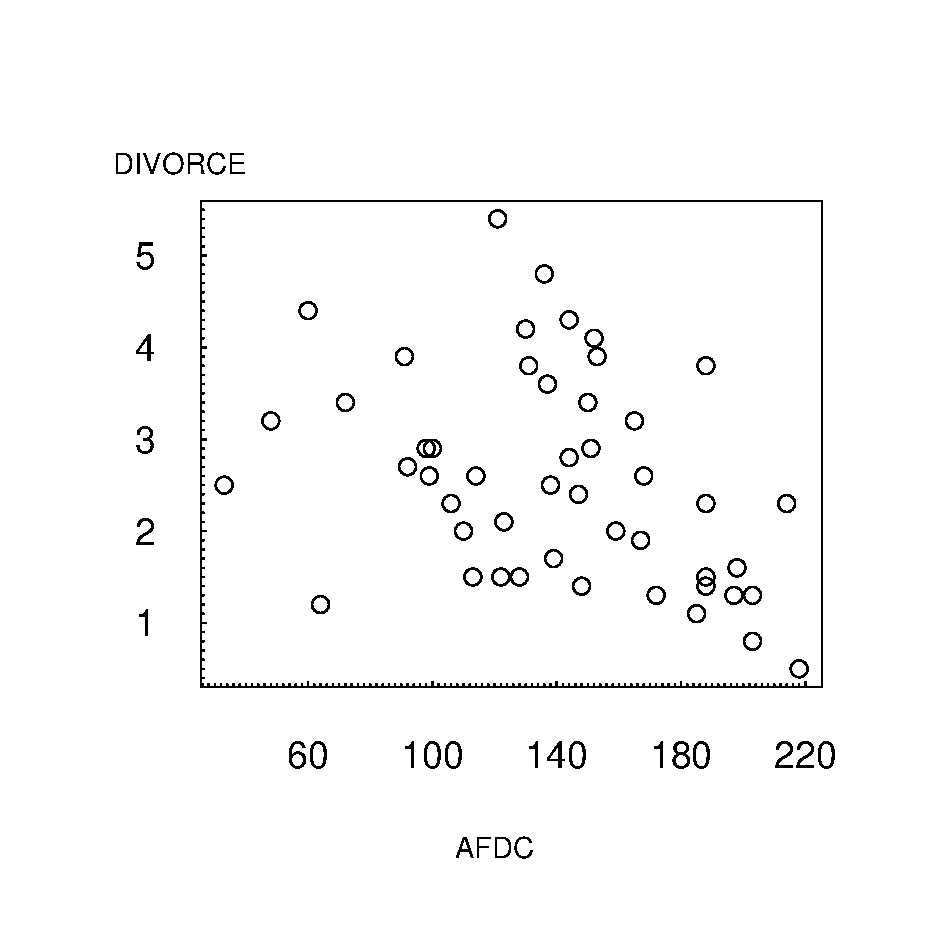
\includegraphics[width=0.45\textwidth]
        {Chapter10LongData/F10Divorce65.eps}
      \hfill
            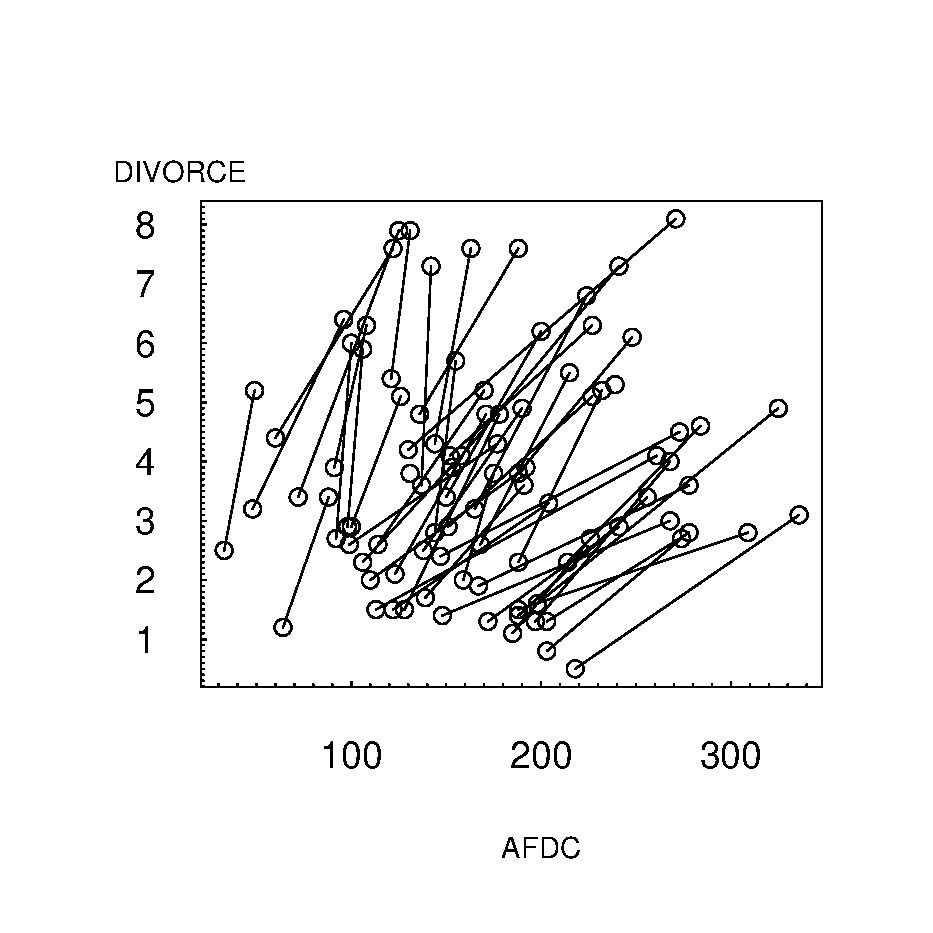
\includegraphics[width=0.45\textwidth]
       {Chapter10LongData/F10DivorcePanel.eps}
      \end{center}
           \parbox[t]{2.5in}{\caption {\label{F10:Divorce}
           {\small Plot of 1965 Divorce versus AFDC Payments.}}} \hfill
        \parbox[t]{2.5in}{\caption {\label{F10:Divorce2}
           {\small Plot of Divorce versus AFDC Payments - 1965 and
           1975.}}}
\end{figure}



Figure \ref{F10:Divorce} shows a negative relation; the
corresponding correlation coefficient is -0.37. Some argue that this
negative relation is counter-intuitive in that one would expect a
positive relation between welfare payments (AFDC) and divorce rates;
states with desirable cultural climates enjoy both low divorce rates
and low welfare payments. Others argue that this negative
relationship is intuitively plausible; wealthy states can afford
high welfare payments and produce economic and cultural climates
conducive to low divorce rates. Because the data are observational,
it is not appropriate to argue for a causal relationship between
welfare payments and divorce rates without additional economic or
sociological theory.

Another plot, not displayed here, shows a similar negative relation
for 1975; the corresponding correlation is -0.425.

Figure \ref{F10:Divorce2} shows both the 1965 and 1975 data; a line
connects the two observations within each state. The line represents
a change over time (dynamic), not a cross-sectional relationship.
Each line displays a positive relationship, that is, as welfare
payments increase so do divorce rates \emph{for each state}. Again,
we do not infer directions of causality from this display. The point
is that the dynamic relation between divorce and welfare payments
\emph{within a state} differs dramatically from the cross-sectional
relationship \emph{between states}.

\linejed

Models of longitudinal data are sometimes differentiated from
regression and time series through their ``double subscripts.'' We
use the subscript $i$ to denote the unit of observation, or
\emph{subject}, and $t$ to denote time. To this end, define $y_{it}$
to be the dependent variable for the $i$th subject during the $t$th
time period. A longitudinal data set consists of observations of the
$i$th subject over $t=1, \ldots, T_i$ time periods, for each of
$i=1, \ldots, n$ subjects. Thus, we observe:
\begin{equation*}
\begin{array}{rl}
    \textrm{first subject} & \{y_{11}, \ldots,  y_{1T_1} \} \\
   \textrm{second subject} & \{y_{21}, \ldots,  y_{2T_2} \} \\
           \multicolumn{1}{c}{\vdots} & \multicolumn{1}{c}{\vdots}  \\
   \textrm{\textit{n}th subject} & \{y_{n1}, \ldots,  y_{nT_n} \} \\
\end{array}
\end{equation*}

In the divorce example, most states have $T_i=2$ observations and
are depicted graphically in Figure \ref{F10:Divorce2} by a line
connecting the two observations. Some states have only $T_i=1$
observation and are depicted graphically by an open circle plotting
symbol. For many data sets, it is useful to let the number of
observations depend on the subject; $T_i$ denotes the number of
observations for the $i$th subject. This situation is known as the
\textit{unbalanced data} case. In other data sets, each subject has
the same number of observations; this is known as the
\textit{balanced data} case.

The applications that we consider are based on many cross-sectional
units and only a few time series replications. That is, we consider
applications where $n$ is large relative to $T = \max (T_1, \ldots,
T_n)$, the maximal number of time periods. Readers will certainly
encounter important applications where the reverse is true, $T > n$,
or where $n \approx T$.


\section{Visualizing Longitudinal and Panel Data}\label{S10:Visual}

To see some ways to visualize longitudinal data, we explore the
following example.

\bigskip


\linejed\index{datasets!Medicare hospital costs}\empexjed{Medicare}

\textbf{Example: Medicare Hospital Costs.} \ecaptionjed{Medicare
hospital costs} We consider $T=6$ years, 1990-1995, of data for
inpatient hospital charges that are covered by the Medicare program.
The data were obtained from the Health Care Financing
Administration. To illustrate, in 1995 the total covered charges
were \$157.8 billions for twelve million discharges. For this
analysis, we use state as the subject, or risk class. Here, we
consider $n=54$ states that include the 50 states in the Union, the
District of Columbia, Virgin Islands, Puerto Rico and an unspecified
``other'' category. The dependent variable of interest is the
severity component, covered claims per discharge, which we label as
CCPD. The variable CCPD is of interest to actuaries because the
Medicare program reimburses hospitals on a per-stay basis. Also,
many managed care plans reimburse hospitals on a per-stay basis.
Because CCPD varies over state and time, both the state and time
(YEAR=1, \ldots, 6) are potentially important explanatory variables.
We do not assume a priori that frequency is independent of severity.
Thus, number of discharges, NUM\_DSCHG, is another potential
explanatory variable. We also investigate the importance of another
component of hospital utilization, AVE\_DAYS, defined to be the
average hospital stay per discharge in days.

\index{plots!multiple time series}\index{plots!scatter plot with
symbols}


Figure \ref{F10:MedicareTSPlot} illustrates the \textit{multiple
time series plot}. Here, we see that not only are overall claims
increasing but also that claims increase for each state. Different
levels of hospitals costs among states are also apparent; we call
this feature \emph{heterogeneity}. Figure \ref{F10:MedicareTSPlot}
indicates that there is greater variability among states than over
time.\index{heterogeneity}


\begin{figure}[htp]
  \begin{center}
    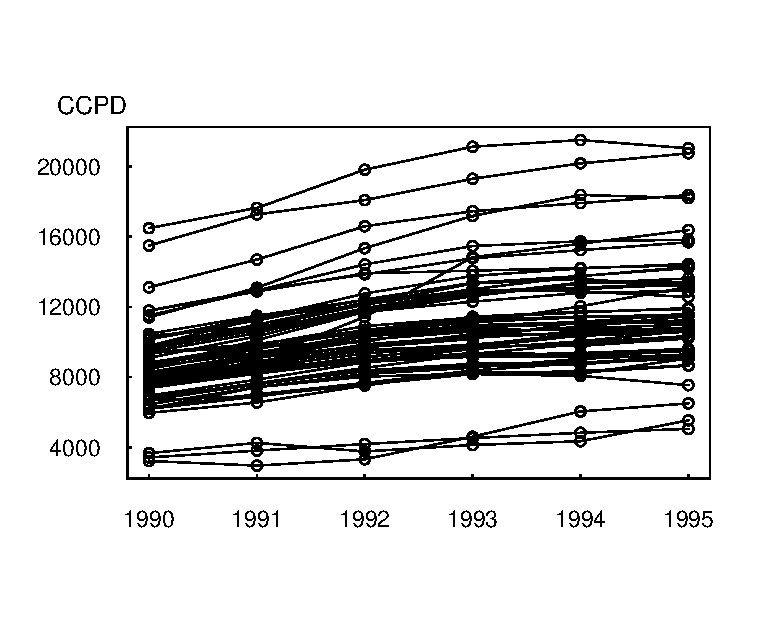
\includegraphics[width=.7\textwidth]
        {Chapter10LongData//F10MedicareTSPlot.eps}
    \caption{\label{F10:MedicareTSPlot} \small Multiple Time Series Plot of CCPD.
    Covered claims per discharge (CCPD) are plotted over $T=6$ years, 1990-1995.
    The line segments connect states; thus, we see that CCPD increases for almost every state over time.}
  \end{center}
\end{figure}



Figure \ref{F10:MedicarePlotWithLines} is a variation of a scatter
plot with symbols. This is a plot of CCPD versus number of
discharges. One could use different plotting symbols each state;
instead, we connect observations within a state over time. This plot
shows a positive overall relationship between CCPD and the number of
discharges. Like CCPD, we see a substantial state variation of
different numbers of discharges. Also like CCPD, the number of
discharges increases over time, so that, for each state, there is a
positive relationship between CCPD and number of discharges. The
slope is higher for those states with smaller number of discharges.
This plot also suggests that the number of discharges lagged by one
year is an important predictor of CCPD.

\begin{figure}[htp]
  \begin{center}
    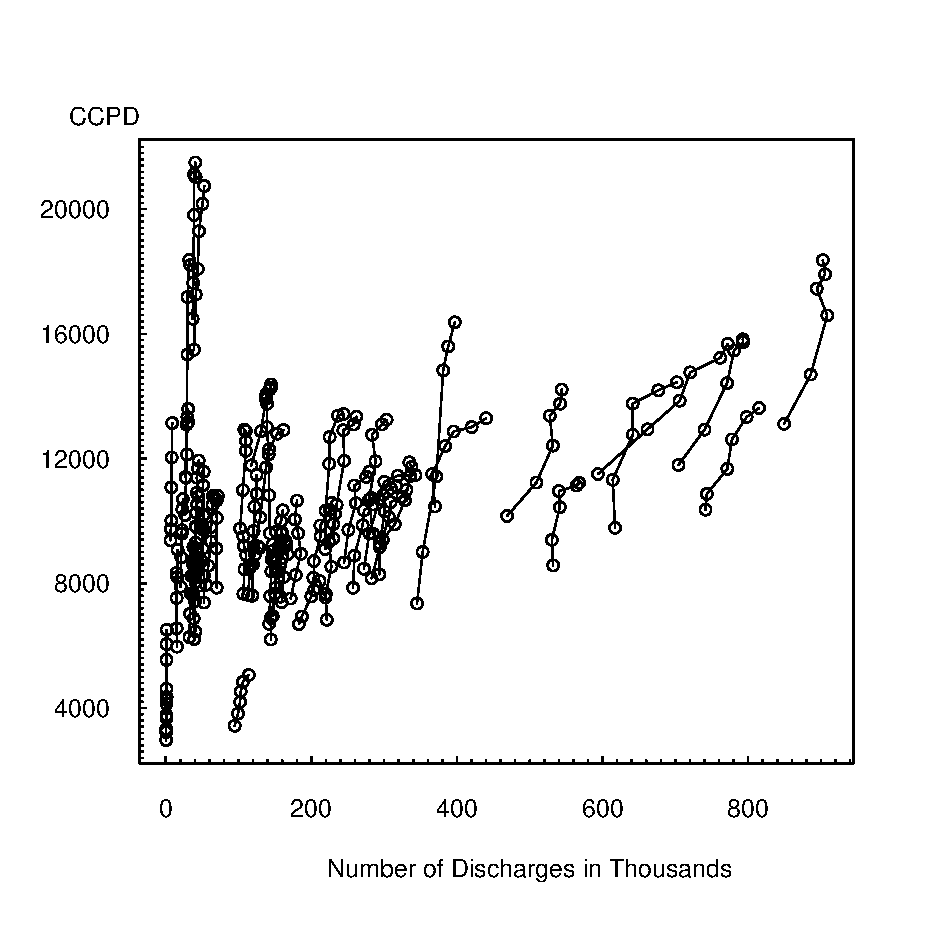
\includegraphics[width=.7\textwidth]
        {Chapter10LongData//F10MedicarePlotWithLines.eps}
    \caption{\label{F10:MedicarePlotWithLines} \small Scatter Plot of CCPD versus Number of Discharges.
    The line segments connect observations within a state over 1990-1995.
    We see a substantial state variation of numbers of discharges.
    There is a positive relationship between CCPD and number of discharges for each state.
    Slopes are higher for those states with smaller number of discharges.}
  \end{center}
\end{figure}


\subsubsection*{Trellis Plot}\index{plots!trellis}

A technique for graphical display that has recently become popular
in the statistical literature is a \emph{trellis plot}. This
graphical technique takes its name from a ``trellis'' which is a
structure of open latticework. When viewing a house or garden, one
typically thinks of a trellis as being used to support creeping
plants such as vines. We will use this lattice structure and refer
to a trellis plot as consisting of one or more panels arranged in a
rectangular array. Graphs that contain multiple versions of a basic
graphical form, each version portraying a variation of the basic
theme, promote comparisons and assessments of change. By repeating a
basic graphical form, we promote the process of communication.

Tufte (1997) states that using small multiples in graphical displays
achieves the same desirable effects as using parallel structure in
writing. Parallel structure in writing is successful because it
allows readers to identify a sentence relationship only once and
then focus on the meaning of each individual sentence element, such
as a word, phrase or clause. Parallel structure helps achieve
economy of expression and draw together related ideas for comparison
and contrast. Similarly, small multiples in graphs allow us to
visualize complex relationships across different groups and over
time. See Guideline Five in Section 21.3 for further discussion.

Figure \ref{F10:MedicareTrellisPlot} illustrates the use of small
multiples. In each panel, the plot portrayed is identical except
that it is based on a different state; this use of parallel
structure allows us to demonstrate the increasing covered claims per
discharge (CCPD) for each state. Moreover, by organizing the states
by average CCPD, we can see the overall level of CCPD for each state
as well as variations in the slope (rate of increase).

\begin{figure}[htp]
  \begin{center}
    \includegraphics[width=.8\textwidth]
        {Chapter10LongData//F10MedicareTrellisPlot.eps}
    \caption{\label{F10:MedicareTrellisPlot} \small Trellis Plot of CCPD versus Year.
    Each of the 54 panels represents a plot of CCPD versus YEAR, 1990-1995 (the horizontal axis is suppressed).
    The increase for New Jersey (NJ) is unusually large.}
  \end{center}
\end{figure}


\linejed

\section{Basic Fixed Effects Models}\label{S10:FEModels}\index{time series models!longitudinal!basic fixed effects}

\subsubsection*{Data}

As described in Section \ref{S10:Intro}, we let $y_{it}$ denote the
dependent variable of the $i$th subject at the $t$th time point.
Associated with each dependent variable is a set of explanatory
variables. For the state hospital costs example, these explanatory
variables include the number of discharged patients and the average
hospital stay per discharge. In general, we assume there are $k$
explanatory variables $x_{it,1}, x_{it,2}, \ldots, x_{it,k}$ that
may vary by subject $i$ and time $t$. We achieve a more compact
notational form by expressing the $k$ explanatory variables as a $k
\times 1$ column vector
\begin{equation*}
\mathbf{x}_{it} = \left(\begin{array}{c}
  x_{it,1} \\
  x_{it,2} \\
  \vdots \\
 x_{it,k}
\end{array}\right) .
\end{equation*}

\noindent With this notation, the data for the $i$th subject
consists of:
\begin{equation*}
\left(\begin{array}{c}
  x_{i1,1},  x_{i1,2}, \ldots,  x_{i1,k}, y_{i1} \\
  \vdots \\
  x_{iT_i,1},  x_{iT_i,2}, \ldots,  x_{iT_i,k}, y_{iT_i} \\
\end{array}\right) = \left(\begin{array}{c}
  \mathbf{x}_{i1}^{\prime}, y_{i1} \\
  \vdots \\
  \mathbf{x}_{iT_i}^{\prime}, y_{iT_i} \\
\end{array}\right) .
\end{equation*}


\subsubsection*{Model}

A basic (and very useful) longitudinal data model is a special case
of the multiple linear regression model introduced in Section 3.2.
We use the modeling assumptions from Section 3.2.3 with the
regression function
\begin{eqnarray}\label{E10:BasicFEModel}
\mathrm{E}~y_{it} & = & \alpha_i + \beta_1 x_{it,1} + \beta_2
x_{it,2} + \cdots + \beta_k x_{it,k} \nonumber\\
& = & \alpha_i + \mathbf{x}_{it}^{\prime} \boldsymbol \beta,~~~~~~
t=1, \ldots, T_i,~~ i=1, \ldots, n .
\end{eqnarray}
This is the \textit{basic fixed effects model}.

The parameters $\{\beta_j\}$ are common to each subject and are
called \emph{global}, or \emph{population}, parameters. The
parameters $\{\alpha_i\}$ vary by subject and are known as
\textit{individual}, or \textit{subject-specific}, parameters. In
many applications, the population parameters capture broad
relationships of interest and hence are the parameters of interest.
The subject-specific parameters account for the different features
of subjects, not broad population patterns. Hence, they are often of
secondary interest and are called \emph{nuisance} parameters. In
Section \ref{S10:REModels}, we will discuss the case where
$\{\alpha_i\}$ are random variables. To distinguish from this case,
this section treats $\{\alpha_i\}$  as non-stochastic parameters
that are called ``fixed effects.''

The subject-specific parameters help to control for differences, or
``heterogeneity'' among subjects. The estimators of these parameters
use information in the repeated measurements on a subject.
Conversely, the parameters $\{\alpha_i\}$ are non-estimable in
cross-sectional regression models without repeated observations.
That is, with $T_i$ = 1, the model $y_{it}  =  \alpha_i + \beta_1
x_{it,1} + \beta_2 x_{it,2} + \cdots + \beta_k x_{it,k} +
\varepsilon_{it}$ has more parameters ($n+k$) than observations
($n$) and thus, we cannot identify all the parameters. Typically,
the disturbance term $\varepsilon_{it}$ includes the information in
$\alpha_i$ in cross-sectional regression models. An important
advantage of longitudinal data models when compared to
cross-sectional regression models is the ability to separate the
effects of  $\{\alpha_i\}$ from the disturbance terms
$\{\varepsilon_{it}\}$. By separating out subject-specific effects,
our estimates of the variability become more precise and we achieve
more accurate inferences.


\subsubsection*{Estimation}

Estimation of the basic fixed effects model follows directly from
the least squares methods. The key insight is that the heterogeneity
parameters $\{\alpha_i\}$ simply represent a \emph{factor}, that is,
a categorical variable that describes the unit of observation. With
this, least squares estimation follows directly with the details
given in Section 4.4 and the supporting appendices.

\marginparjed{The heterogeneity parameters $\{\alpha_i\}$ can be
represented by a \emph{factor}, that is, a categorical variable that
describes the unit of observation.}\index{time series
models!longitudinal!least squares dummy variable}

As described in Chapter 4, one can replace categorical variables
with an appropriate set of binary variables. For this reason, panel
data estimators are sometimes known as \emph{least squares dummy
variable model} estimators. However, as we have seen in Chapter 4,
be careful on the statistical routines. For some applications, the
number of subjects can easily run into the thousands. Creating this
many binary variables is computationally cumbersome. When you
identify a variable as categorical, statistical packages typically
use more computationally efficient recursive procedures (described
in Section 4.7.2).

\marginparjed{In the basic fixed effects model, coefficients
associated with time-constant variables cannot be estimated.}

The heterogeneity factor $\{ \alpha_i \}$ does not depend on time.
Because of this, it is easy to establish that regression
coefficients associated with time-constant variables cannot be
estimated using the basic fixed effects model. In other words,
time-constant variables are perfectly collinear with the
heterogeneity factor. Because of this limitation, analysts often
prefer to design their studies to use the competing random effects
model that we will describe in Section \ref{S10:REModels}.

\newpage

\linejed

\textbf{Example: Medicare Hospital Costs - Continued.} We compare
the fit of the basic fixed effects model to ordinary regression
models. Model 1 of Table \ref{T10:MedicareRegression} shows the fit
of an ordinary regression model using number of discharges
(NUM\_DCHG), YEAR and average hospital stay (AVE\_DAYS). Judging by
the large $t$-statistics, each variable is statistically
significant. The intercept term is not printed.

Figure \ref{F10:MedicareTrellisPlot} suggests that New Jersey has an
unusually large increase. Thus, an interaction term, YEARNJ, was
created that equals YEAR if the observation is from New Jersey and
zero otherwise. This variable is incorporated in Model 2 where it
does not appear to be significant.

Table \ref{T10:MedicareRegression} also shows the fit of a basic
fixed effects model with these explanatory variables. In the table,
the 54 subject-specific coefficients are not reported. In this
model, each variable is statistically significantly, including the
interaction term. Most striking is the improvement in the overall
fit. The residual standard deviation ($s$) decrease from 2,731 to
530 and the coefficient of determination ($R^2$) increased from 29\%
to 99.8\%.



\begin{table}[h]
\scalefont{0.9} \caption{\label{T10:MedicareRegression} \small
Coefficients and Summary Statistics from Three Models}
\begin{tabular}{lrrrrrr}
\hline
 &\multicolumn{2}{c}{Regression}&\multicolumn{2}{c}{Regression}&\multicolumn{2}{c}{Basic Fixed} \\
 &\multicolumn{2}{c}{Model 1} &\multicolumn{2}{c}{Model 2}
 &\multicolumn{2}{c}{Effects Model} \\
 & Coefficient & $t$-statistic &Coefficient & $t$-statistic &Coefficient & $t$-statistic
 \\
 \hline
  NUM\_DCHG &       4.70 &       6.49 &       4.66 &       6.44 &      10.75 &       4.18 \\
      YEAR &     744.15 &       7.96 &     733.27 &       7.79 &     710.88 &      26.51 \\
  AVE\_DAYS &     325.16 &       3.85 &     308.47 &       3.58 &     361.29 &       6.23 \\
      YEARNJ &            &            &     299.93 &       1.01 &   1,262.46 &       9.82 \\
      \hline
     $s$ &   \multicolumn{2}{c}{2,731.90} &  \multicolumn{2}{c}{2,731.78} &  \multicolumn{2}{c}{529.45}            \\
        $R^2$ (in percent) &  \multicolumn{2}{c}{28.6} &  \multicolumn{2}{c}{28.8} & \multicolumn{2}{c}{99.8}        \\
        $R_a^2$ (in percent) &  \multicolumn{2}{c}{27.9} &  \multicolumn{2}{c}{27.9} & \multicolumn{2}{c}{99.8}        \\
        \hline
\end{tabular}
\scalefont{1.1111}
\end{table}


\linejed

\section{Extended Fixed Effects Models}\label{S10:FEModels2}\index{time series models!longitudinal!extended fixed effects}

\subsubsection*{Analysis of Covariance Models}

In the basic fixed effects model, no special relationships between
subjects and time periods are assumed. By interchanging the roles of
``$i$'' and ``$t$'', we may consider the regression function
\begin{equation*}
\mathrm{E}~y_{it} = \lambda_t + \mathbf{x}_{it}^{\prime} \boldsymbol
\beta.
\end{equation*}\index{time series
models!longitudinal!one-way fixed effects} Both this regression
function and the one in equation (\ref{E10:BasicFEModel}) are based
on traditional one-way analysis of covariance models introduced in
Section 4.4. For this reason, the basic fixed effects model is also
called the \emph{one-way fixed effects model}. By using binary
(dummy) variables for the time dimension, we can incorporate
time-specific parameters into the population parameters. In this
way, it is straightforward to consider the regression function
\begin{equation*}
\mathrm{E}~y_{it} = \alpha_i + \lambda_t + \mathbf{x}_{it}^{\prime}
\boldsymbol \beta ,
\end{equation*}
known as the \emph{two-way fixed effects model}.\index{time series
models!longitudinal!two-way fixed effects}

\bigskip
\linejed

\textbf{Example: Urban Wages.} Glaeser and Mar\'{e} (2001)
investigated the effects of determinants on wages, with the goal of
understanding why workers in cities earn more than their non-urban
counterparts. They examined two-way fixed effects models using data
from the National Longitudinal Survey of Youth (NLSY); they also
used data from the Panel Study of Income Dynamics (PSID) to assess
the robustness of their results to another sample. For the NLSY
data, they examined $n = 5,405$ male heads of households over the
years 1983-1993, consisting of a total of $N = 40,194$ observations.
The dependent variable was logarithmic hourly wage. The primary
explanatory variable of interest was a three level categorical
variable that measures the city size in which workers reside. To
capture this variable, two binary (dummy) variables were used: (1) a
variable to indicate whether the worker resides in a large city
(with more than one-half million residents), a ``dense metropolitan
area,'' and (2) a variable to indicate whether the worker resides in
a metropolitan area that does not contain a large city, a
``non-dense metropolitan area.'' The reference level is
non-metropolitan area. Several other control variables were included
to capture effects of a worker's experience, occupation, education
and race. When including time dummy variables, there were $k = 30$
explanatory variables in the reported regressions.

\linejed

\subsubsection*{Variable Coefficients Models}

In the Medicare hospital costs example, we introduced an interaction
variable to represent the unusually high increases in New Jersey
costs. However, an examination of Figure
\ref{F10:MedicareTrellisPlot} suggests that many other states are
also ``unusual.'' Extending this line of thought, we might wish to
allow each state to have its own rate of increase, corresponding to
the increased hospital charges for that state. We could consider a
regression function of the form
\begin{equation}\label{E10:MedicareVSlope}
\mathrm{E}~CCPD_{it} = \alpha_i + \beta_1 (NUM\_DCHG)_{it} +
\beta_{2i} (YEAR)_{t} + \beta_3 (AVE\_DAYS)_{it} ,
\end{equation}
where the slope associated with YEAR is allowed to vary with state
``$i$.''

Extending this line of thought, we write the regression function for
a \emph{variable coefficients} fixed effects model as\index{time
series models!longitudinal!variable coefficients}
\begin{equation*}
\mathrm{E}~y_{it} =  \mathbf{x}_{it}^{\prime} \boldsymbol \beta_i.
\end{equation*}
With this notation, we may allow any or all of the variables to be
associated with subject-specific coefficients. For simplicity, the
subject-specific intercept is now included in the regression
coefficient vector $ \boldsymbol \beta_i$.

\linejed

\textbf{Example: Medicare Hospital Costs - Continued.} The
regression function in equation (\ref{E10:MedicareVSlope}) was fit
to the data. Not surprisingly, it resulted in excellent fit in the
sense that the coefficient of determination is $R^2 = 99.915 \% $
and the adjusted version is $R_a^2 = 99.987 \% $. However, compared
to the basic fixed effects model, there are an additional 52
parameters, a slope for each state (54 states to begin with, minus
one for the `population' term and minus one for New Jersey already
included). Are the extra terms helpful? One way of analyzing this is
through the general linear hypothesis test introduced in Section
4.2.2. In this context, the variable coefficients model represents
the ``full'' equation and the basic fixed effects model is our
``reduced'' equation. From equation (4.4), the test statistic is
\begin{equation*}
F-\textrm{ratio} = \frac {(0.99915 - 0.99809)/52}{(1-0.99915)/213} =
5.11 .
\end{equation*}
Comparing this to the $F$-distribution with $df_1 = 52$ and $df_2 =
213$, we see that the associated $p$-value is less than 0.0001,
indicating strong statistical significance. Thus, this is one
indication that the variable slope model is preferred when compared
to the basic fixed effects model.

\linejed


\subsubsection*{Models with Serial Correlation}

In longitudinal data, subjects are measured repeatedly over time.
For some applications, time trends represent a minor portion of the
overall variation. In these cases, one can adjust for their presence
by calculating standard errors of regression coefficients robustly,
similar to the Section 5.7.2 discussion. However, for other
applications, getting a good understanding of time trends is vital.
One such application that is important in actuarial science is
prediction; for example, recall the Section \ref{S10:Intro}
discussion of an actuary predicting insurance claims for a small
business.

We have seen in Chapters 7--9 some basic ways to incorporate time
trends, through linear trends in time (such as the YEAR term in the
Medicare hospital costs example) or using dummy variables in time
(another type of one-way fixed effects model). Another possibility
is to use a lagged dependent variable as a predictor. However, this
is known to have some unexpected negative consequences for the basic
fixed effects model (see for example the discussion in Hsiao, 2003,
Section 4.2 or Frees, 2004, Section 6.3).

Instead, it is customary to examine the serial correlation structure
of the disturbance term $ \varepsilon_{it} = y_{it} -
\mathrm{E}~y_{it}.$ For example, a common specification is to use an
autocorrelation of order one, $AR(1)$, structure, such as
\begin{equation*}
\varepsilon_{it} = \rho_{\varepsilon} \varepsilon_{i,t-1} +
\eta_{it},
\end{equation*}
where $\{ \eta_{it} \}$ is a set of disturbance random variables and
$\rho_{\varepsilon}$ is the autocorrelation parameter. In many
longitudinal datasets, the small number of time measurements ($T$)
would inhibit calculation of the correlation coefficient
$\rho_{\varepsilon}$ using traditional methods such as those
introduced in Chapter 8. However, with longitudinal data, we have
many replications ($n$) of these short times series; intuitively,
these replications provide the information needed to provide
reliable estimates of the autoregressive parameter.


\section{Random Effects Models}\label{S10:REModels}\index{time series models!longitudinal!random effects}


Suppose that you are interested in studying the behavior of subjects
that are randomly selected from a population. For example, you might
wish to predict insurance claims for a small business, using
characteristics of the business as well as past claims history.
Here, the set of small businesses may be randomly selected from a
larger database. In contrast, the Section \ref{S10:FEModels}
Medicare example dealt with a fixed set of subjects. That is, it is
difficult to think of the 54 states as a subset from some
``super-population'' of states. For both situations, it is natural
to use subject-specific parameters, $\{\alpha_i \}$, to represent
the heterogeneity among subjects. Unlike Section \ref{S10:FEModels},
we now discuss situations in which it is more reasonable to
represent $\{\alpha_i \}$ as random variables instead of fixed, yet
unknown, parameters. By arguing that $\{\alpha_i \}$ are draws from
a distribution, we will have the ability to make inferences about
subjects in a population that are not included in the sample.

\subsubsection*{Basic Random Effects Model}\index{time
series models!longitudinal!basic random effects}

The \emph{basic random effects} model equation is
\begin{equation}\label{E10:BasicREModel}
y_{it} = \alpha_i + \mathbf{x}_{it}^{\prime} \boldsymbol \beta +
\varepsilon_{it},~~~~~~ t=1, \ldots, T_i,~~ i=1, \ldots, n .
\end{equation}
This notation is similar to the basic fixed effects model. However,
now the term $\alpha_i$ is assumed to be a random variable, not a
fixed, unknown parameter. The term $\alpha_i$ is known as a
\emph{random effect}. \emph{Mixed effects} models are ones that
include random as well as fixed effects. Because equation
(\ref{E10:BasicREModel}) includes random effects ($\alpha_i$) and
fixed effects ($\mathbf{x}_{it}$), the basic random effects model is
a special case of the \emph{mixed linear model}. The general mixed
linear model is introduced in Section 15.1.

To complete the specification, we assume that $\{\alpha_i \}$  are
identically and independently distributed with mean zero and
variance $\sigma_{\alpha}^2$. Further, we assume that $\{\alpha_i
\}$ are independent of the disturbance random variables,
$\varepsilon_{it}$. Note that because E $\alpha_i$ = 0, it is
customary to include a constant within the vector $\mathbf{x}_{it}$.
This was not true of the fixed effects models in Section
\ref{S10:FEModels} where we did not center the subject-specific
terms about 0.

Linear combinations of the form $\mathbf{x}_{it}^{\prime}
\boldsymbol \beta $ quantify the effect of known variables that may
affect the dependent variable. Additional variables, that are either
unimportant or unobservable, comprise the ``error term.'' In
equation (\ref{E10:BasicREModel}), we may think of a regression
model $y_{it} = \mathbf{x}_{it}^{\prime} \boldsymbol \beta +
\eta_{it},$ where the error term $\eta_{it}$ is decomposed into two
components so that $\eta_{it}= \alpha_i + \varepsilon_{it}$. The
term $\alpha_i$ represents the time-constant portion whereas
$\varepsilon_{it}$ represents the remaining portion. To identify the
model parameters, we assume that the two terms are independent. In
the econometrics literature, this is known as the \emph{error
components} model; in the biological sciences, is is known as the
\emph{random intercepts} model.

\subsubsection*{Estimation}

Estimation of the random effects model does not follows directly
from least squares as with the fixed effects models. This is because
the observations are no longer independent due to the random effects
terms. Instead, an extension of least squares known as
\emph{generalized least squares} is used to account for this
dependency. Generalized least squares, often denoted by the acronym
\emph{GLS}, is a type of weighted least squares. Because random
effects models are special cases of mixed linear models, we will
introduce GLS estimation in this broader framework in Section 15.1.

To see the dependency among observations, consider the covariance
between the first two observations of the $i$th subject. Basic
calculations show

\begin{eqnarray*}
\mathrm{Cov}(y_{i1}, y_{i2}) &= &\mathrm{Cov}(\alpha_i +
\mathbf{x}_{i1}^{\prime} \boldsymbol \beta + \varepsilon_{i1},
\alpha_i + \mathbf{x}_{i2}^{\prime} \boldsymbol \beta +
\varepsilon_{i2}) \\
&= &\mathrm{Cov}(\alpha_i +\varepsilon_{i1}, \alpha_i +
 \varepsilon_{i2}) \\&= &\mathrm{Cov}(\alpha_i , \alpha_i)+\mathrm{Cov}(\alpha_i,
 \varepsilon_{i2})+\mathrm{Cov}(\varepsilon_{i1}, \alpha_i)+\mathrm{Cov}(\varepsilon_{i1},
 \varepsilon_{i2}) \\
 &= & \mathrm{Cov}(\alpha_i , \alpha_i) = \sigma^2_{\alpha} .
\end{eqnarray*}
The systematic terms $\mathbf{x}^{\prime} \boldsymbol \beta $ drop
out of the covariance calculation because they are non-random.
Further, the covariance terms involving $\varepsilon$ are zero
because of the assumed independence. This calculation shows that the
covariance between any two observations from the same subject is $
\sigma^2_{\alpha} $. Similar calculations show that the variance of
an observation is $\sigma^2_{\alpha} +\sigma^2_{\varepsilon}.$ Thus,
the correlation between observations within a subject is
$\sigma^2_{\alpha} / (\sigma^2_{\alpha} +\sigma^2_{\varepsilon})$.
This quantity is known as the \emph{intra-class correlation}, a
commonly reported measure of dependence in random effects studies.


\linejed

\textbf{Example: Group Term Life.} \ecaptionjed{Group Term Life}
Frees, Young and Luo (2001) analyzed claims data provided by an
insurer of credit unions. The data contains claims and exposure
information from 88 Florida credit unions for years 1993-1996. These
are ``life savings'' claims from a contract between the credit union
and their members that provides a death benefit based on the
member's savings deposited in the credit union. Actuaries typically
price life insurance coverage with knowledge of an insureds' age and
gender, as well as other explanatory variables such as occupation.
However, for these data from small groups, often only a minimal
amount of information is available to understand claims behavior.

Of the $88 \times 4=352$ potential observations, 27 were not
available because these credit unions had zero coverage in that year
(and thus excluded). Thus, these data were unbalanced. The dependent
variable is the annual total claims from the life savings contract,
in logarithmic units. The explanatory variables were annual
coverage, in logarithmic units, and YEAR, a time trend.

A fit of the basic random effects model showed that both year and
the annual coverage had positive and  strongly statistically
significant coefficients. That is, the typical amount of claims
increased over the period studied and claims increased as coverage
increased, other things being equal. There were strong credit union
effects, as well. For example, the estimated intra-class correlation
was 0.703, also suggesting strong dependence among observations.

\linejed

\subsubsection*{Extended Random Effects Models}\index{time
series models!longitudinal!extended random effects}

Just as with fixed effects, random effects models can be easily
extended to incorporated variable coefficients and serial
correlations. For example, Frees et al. (2001) considered the model
equation
\begin{equation}\label{E10:REExample}
y_{it} = \alpha_{1i} + \alpha_{2i} \mathrm{LNCoverage}_{it}+ \beta_1
+ \beta_2 \mathrm{YEAR}_t+ \beta_3 \mathrm{LNCoverage}_{it}+
\varepsilon_{it} ,
\end{equation}
where $\mathrm{LNCoverage}_{it}$ is the logarithmic life savings
coverage. As with the basic model, it is customary to use a mean
zero for the random effects. Thus, the overall intercept is
$\beta_1$ and $\alpha_{1i}$ represents credit union deviations.
Further, the overall or global slope associated with
$\mathrm{LNCoverage}$ is $\beta_3$ and $\alpha_{2i}$ represents
credit union deviations. Put another way, the slope corresponding to
$\mathrm{LNCoverage}$ for the $i$th credit is $\beta_3 +
\alpha_{2i}$.

More generally, the \emph{variable coefficients random effects
model} equation can be written as
\begin{equation}\label{E10:REModel}
y_{it} = \mathbf{x}_{it}^{\prime} \boldsymbol \beta +
\mathbf{z}_{it}^{\prime} \boldsymbol \alpha _i + \varepsilon_{it}.
\end{equation}
As with the fixed effects variable coefficients model, we may allow
any or all of the variables to be associated with subject-specific
coefficients. The convention used in the literature is to specific
fixed effects through the systematic component
$\mathbf{x}_{it}^{\prime} \boldsymbol \beta$ and random effects
through the component $\mathbf{z}_{it}^{\prime} \boldsymbol \alpha
_i$. Here, the vector $\mathbf{z}_{it}$ is typically equal to or a
subset of $\mathbf{x}_{it}$ although it need not be so. With this
notation, we now have a vector of random effects $\boldsymbol \alpha
_i$ that are subject-specific. To reduce to our basic model, one
only needs to choose $\boldsymbol \alpha _i$ to be a scalar (a $1
\times 1$ vector) and $\mathbf{z}_{it}\equiv 1.$ The example in
equation (\ref{E10:REExample}) results from choosing $\boldsymbol
\alpha _i = (\alpha_{1i}, \alpha_{2i})^{\prime}$ and
$\mathbf{z}_{it} = (1, \mathrm{LNCoverage}_{it})^{\prime}$.

As with fixed effects models, one can readily incorporate models of
serial correlation into random effects models by specifying a
correlations structure for $\varepsilon_{i1}, \ldots,
\varepsilon_{iT}$. This feature is readily available in statistical
packages and is described fully in the Section \ref{S10:References}
references.



\section{Further Reading and References}\label{S10:References}

Longitudinal and panel data models are widely used. To illustrate,
an index of business and economic journals, \textit{ABI/INFORM},
lists 685 articles in 2004 and 2005 that use panel data methods.
Another index of scientific journals, the \textit{ISI Web of
Science}, lists 1,137 articles in 2004 and 2005 that use
longitudinal data methods. A book-long introduction to longitudinal
and panel data that emphasizes business and social science
applications is Frees (2004). Diggle et al. (2002) provides an
introduction from a biomedical perspective. Hsiao (2003) provides a
classic introduction from an econometric perspective.

Actuaries are particularly interested in predictions resulting from
longitudinal data. These predictions can form the basis for updating
insurance prices. This topic is discussed in Chapter 18 on
credibility and bonus-malus factors.\index{actuarial \& financial
terms and concepts!credibility}



\bigskip

\textbf{Chapter References}

\begin{multicols}{2}

\scalefont{0.9}

Diggle, Peter J., Patrick Heagarty, Kung-Yee Liang and Scott L.
Zeger (2002). \textit{Analysis of Longitudinal Data, Second
Edition}. Oxford University Press, London.

Frees, Edward W. (2004). \textit{Longitudinal and Panel Data:
Analysis and Applications in the Social Sciences.} Cambridge
University Press, New York.

Frees, Edward W., Virginia R. Young and Yu Luo (2001). Case studies
using panel data models. \emph{North American Actuarial Journal} 5
(4), 24-42.

Glaeser, E. L. and D. C. Mar\'{e} (2001). Cities and skills.
\emph{Journal of Labor Economics} 19, 316-342.

Hsiao, Cheng (2003). \textit{ Analysis of Panel Data, Second
Edition}. Cambridge University Press, New York.

Tufte, Edward R. (1997). \emph{Visual Explanations}. Cheshire,
Conn.: Graphics Press.




\scalefont{1.1111}

\end{multicols}


\part{Topics in Nonlinear Regression}
\setcounter{chapter}{10}
\chapter{Categorical Dependent Variables}
{\small \textit{Chapter Preview}. A model with a categorical
dependent variable allows one to predict whether an observation is a
member of a distinct group, or category. Binary variables represent
an important special case; they can indicate whether or not an event
of interest has occurred. In actuarial and financial applications,
the event may be whether a claim occurs, a person purchases
insurance, a person retires or a firm becomes insolvent. The chapter
introduces logistic regression and probit models of binary dependent
variables. Categorical variables may also represent more than two
groups, known as \emph{multicategory} outcomes. Multicategory
variables may be unordered or ordered, depending on whether it makes
sense to rank the variable outcomes. For unordered outcomes, known
as \emph{nominal} variables, the chapter introduces generalized
logits and multinomial logit models. For ordered outcomes, known as
\emph{ordinal} variables, the chapter introduces cumulative logit
and probit models.}

\section{Binary Dependent Variables}

We have already introduced binary variables as a special type of
discrete variable that can be used to indicate whether or not a
subject has a characteristic of interest, such as gender for a
person or ownership of a captive insurance company for a firm.
Binary variables also describe whether or not an event of interest
has occurred, such as an accident. A model with a binary dependent
variable allows one to predict whether an event has occurred or a
subject has a characteristic of interest.\index{categorical
variable!binary}

\linejed

\textbf{Example: MEPS Expenditures.}\ecaptionjed{MEPS Expenditures}
Section \ref{S11:MEPS} will describe an extensive database from the
Medical Expenditure Panel Survey (MEPS) on hospitalization
utilization and expenditures. For these data, we will consider
\begin{equation*}
y_i = \left\{
\begin{array}{ll}
1 & i\text{th person was hospitalized during the sample period} \\
0 & \text{otherwise}%
\end{array}%
\right. .
\end{equation*}%
There are $n=2,000$ persons in this sample, distributed as:
\vspace{-.2in}
 \scalefont{0.9}  \begin{center}  \begin{table}[h]
\caption{\label{T11:MEPSIntroStats} Hospitalization by Gender}
\begin{tabular}{ll|ll}
\hline
 &  &  Male & Female   \\ \hline
Not hospitalized & $y=0$ & 902 (95.3\%) & ~~941 (89.3\%)\\
Hospitalized & $y=1$ &  ~44 ( 4.7\%)  & ~~113 (10.7\%)\\
 Total &       & 946  & 1,054 \\
 \hline
\end{tabular}
\end{table}  \end{center}  \scalefont{1.1111}
\noindent Table \ref{T11:MEPSIntroStats} suggests that gender has an
important influence on whether someone becomes hospitalized.

\linejed
\bigskip

Like the linear regression techniques introduced in prior chapters, we are
interested in using characteristics of a person, such as their age, sex,
education, income and prior health status, to help explain the
dependent variable $y$. Unlike the prior chapters, now the dependent
variable is discrete and not even approximately normally distributed. In
limited circumstances, linear regression can be used with binary dependent
variables - this application is known as a \emph{linear probability model}.

\subsubsection*{Linear probability models}\index{regression model!linear
probability}\index{symbols!$\pi_i$, probability of a 1 for subject
$i$}

To introduce some of the complexities encountered with binary
dependent variables, denote the probability that the response equals
1 by $\pi_i= \mathrm{Pr}(y_i=1)$. A binary random
variable has a \emph{Bernoulli distribution}. Thus, we may interpret
the mean response as the probability that the response equals
one, that is, $\mathrm{E~}y_i=0\times \mathrm{Pr}(y_i=0) + 1 \times
\mathrm{Pr}(y_i=1) = \pi_i$. Further, the variance is related to the
mean through the expression $\mathrm{Var}~y_i = \pi_i(1-\pi_i)$.

\marginparjed{Linear probability models enjoy convenient parameter
interpretations.}

We begin by considering a linear model of the form%
\begin{equation*}
y_i = \mathbf{x}_i^{\mathbf{\prime}} \boldsymbol \beta +
\varepsilon_i,
\end{equation*}
known as a linear probability model. Assuming
$\mathrm{E~}\varepsilon_i=0$, we have that
$\mathrm{E~}y_i=\mathbf{x}_i^{\mathbf{\prime }} \boldsymbol \beta
=\pi_i$. Because $y_i$ has a Bernoulli distribution,
$\mathrm{Var}~y_i=\mathbf{x}_i^{\mathbf{\prime}} \boldsymbol
\beta(1-\mathbf{x}_i^{\mathbf{\prime}}\boldsymbol \beta)$. Linear
probability models are used because of the ease of parameter
interpretations. For large data sets, the computational simplicity
of ordinary least squares estimators is attractive when compared to
some complex alternative nonlinear models introduced later in this
chapter. As described in Chapter 3, ordinary least squares
estimators for $\boldsymbol \beta$ have desirable properties. It is
straightforward to check that the estimators are consistent and
asymptotically normal under mild conditions on the explanatory
variables \{$\mathbf{x}_i$\}. However, linear probability models
have several drawbacks that are serious for many applications.

\bigskip

\boxedjed

\textit{Drawbacks of the Linear Probability Model}

\begin{itemize}
\item \emph{Fitted values can be poor.} The expected response is a probability and thus must vary between 0
and 1. However, the linear combination,
$\mathbf{x}_i^{\mathbf{\prime}} \boldsymbol \beta$, can vary between
negative and positive infinity. This mismatch implies, for example,
that fitted values may be unreasonable.

\item \emph{Heteroscedasticity.} Linear models assume homoscedasticity (constant variance) yet the
variance of the response depends on the mean that varies over
observations. The problem of varying variability is known as
heteroscedasticity.\index{heteroscedasticity}

\item \emph{Residual analysis is meaningless.} The response must be either a 0 or 1 although the regression models
typically regards distribution of the error term as continuous. This
mismatch implies, for example, that the usual residual analysis in
regression modeling is meaningless.
\end{itemize}

\end{boxedminipage}
\bigskip

To handle the heteroscedasticity problem, a (two-stage) weighted
least squares procedure is possible. In the first stage,
one uses ordinary least squares to compute estimates of $\boldsymbol
\beta$. With this estimate, an estimated variance for each subject
can be computed using the
relation $\mathrm{Var}~y_i=\mathbf{x}_i^{\mathbf{\prime}}\boldsymbol \beta%
(1-\mathbf{x}_i^{\mathbf{\prime}}\boldsymbol \beta)$. At the second
stage, a weighted least squares is performed using the inverse of
the estimated variances as weights to arrive at new estimates of
$\boldsymbol \beta$. It is possible to iterate this procedure,
although studies have shown that there are few advantages in doing
so (see Carroll and Ruppert, 1988). Alternatively, one can use
ordinary least squares estimators of $\boldsymbol \beta$ with
standard errors that are robust to heteroscedasticity (see Section
5.7.2).\index{heteroscedasticity-consistent standard error}

\section{Logistic and Probit Regression
Models}\label{S11:LogProbModels}\index{regression
model!logistic}\index{regression
model!probit}\index{symbols!$\mathrm{\pi}(\cdot)$, probability
function}

\subsection{Using Nonlinear Functions of Explanatory Variables}

To circumvent the drawbacks of linear probability models, we consider
alternative models in which we express the expectation of the response as a
function of explanatory variables, $\pi_i=\mathrm{\pi }(\mathbf{x}_i^{%
\mathbf{\prime}}\boldsymbol \beta)=\Pr (y_i=1|\mathbf{x}_i)$. We
focus on two special cases of the function $\mathrm{\pi
}(\cdot)$:

\begin{itemize}
\item $\mathrm{\pi }(z)=\frac{1}{1+\exp (-z)}=\frac{e^{z}}{1+e^{z}}$, the
logit case, and

\item $\mathrm{\pi }(z)=\mathrm{\Phi }(z)$, the probit case.
\end{itemize}

\noindent Here, $\mathrm{\Phi }(\cdot)$ is the standard normal
distribution function. The choice of the identity function (a
special kind of linear function), $\mathrm{\pi }(z)=z$, yields the
linear probability model. In contrast, $\mathrm{\pi}$ is nonlinear
for both the logit and probit cases. These two functions are similar
in that they are almost linearly related over the interval $0.1\leq
p\leq 0.9$. Thus, to a large extent, the function choice is
dependent on the preferences of the analyst. Figure
\ref{F11:LogitProbit} compares the logit and probit functions
showing that it will be difficult to distinguish between the two
specifications with most data sets.


The inverse of the function, $\mathrm{\pi }^{-1}$, specifies the
form of the probability that is linear in the explanatory variables,
that is, $\mathrm{\pi }^{-1}(\pi_i)=
\mathbf{x}_i^{\mathbf{\prime}}\boldsymbol \beta$. In Chapter 13, we
refer to this inverse as the \emph{link function}.\index{link
function}


\begin{figure}[htp]
  \begin{center}
    \includegraphics[width=1\textwidth,angle=0,scale=0.5]{Chapter11Binary/F11LogitProbit.eps}
    \caption{\label{F11:LogitProbit} \small Comparison of Logit and Probit (Standard Normal) Distribution
Functions}
  \end{center}
\end{figure}


\linejed\index{actuarial \& financial terms and concepts!credit
scoring}\index{examples!credit scores}

\textbf{Example: Credit Scoring.}\ecaptionjed{Credit Scoring} Banks,
credit bureaus and other financial institutions develop ``credit
scores'' for individuals that are used to predict the likelihood
that the borrower will repay current and future debts. Individuals who
do not meet stipulated repayment schedules in a loan agreement are
said to be in ``default.'' A credit score is then a predicted
probability of being in default, with the credit application
providing the explanatory variables used in developing the credit
score. The choice of explanatory variables depends on the purpose of
the application; credit scoring is used for issuing credit cards for
making small consumer purchases as well as mortgage applications for
multimillion dollar houses. In Table
\ref{T11:CreditCharacteristics}, Hand and Henley (1997) provide a
list of typical characteristics that are used in credit scoring.


\scalefont{0.9}
\begin{table}[h]
\caption{\label{T11:CreditCharacteristics} Characteristics Used in
Some Credit Scoring Procedures}
\begin{tabular}{ll}
   \hline
Characteristics & Potential Values \\
\hline Time at present address & 0-1, 1-2, 3-4, 5+ years \\
Home status & Owner, tenant, other \\
Postal Code & Band A, B, C, D, E \\
Telephone & Yes, no \\
Applicant's annual income & \pounds (0-10000), \pounds
(10,000-20,000)
\pounds(20,000+) \\
Credit card & Yes, no \\
Type of bank account & Check and/or savings, none \\
Age & 18-25, 26-40, 41-55, 55+ years \\
County Court judgements & Number \\
Type of occupation & Coded \\
Purpose of loan & Coded \\
Marital status & Married, divorced, single, widow, other \\
Time with bank & Years \\
Time with employer & Years \\
 \hline
     \multicolumn{2}{c}{\textit{Source}: Hand and Henley (1997)} \\
\end{tabular}
\end{table}
\scalefont{1.1111}

\bigskip

With credit application information and default experience, a
logistic regression model can be used to fit the probability of
default with credit scores resulting from fitted values. Wiginton
(1980) provides an early application of logistic regression to
consumer credit scoring. At that time, other statistical methods
known as discriminant analysis were at the cutting edge of
quantitative scoring methodologies. In their review article, Hand
and Henley (1997) discuss other competitors to logistic regression
including machine learning systems and neural networks. As noted by
Hand and Henley, there is no uniformly ``best'' method. Regression
techniques are important in their own right due to their widespread
usage and because they can provide a platform for learning about
newer methods.

\marginparjed{Regression techniques are important due to their
widespread usage and because they can provide a platform for
learning about newer methods.}

Credit scores provide estimates of the likelihood of defaulting on
loans but issuers of credit are also interested in the amount and
timing of debt repayment. For example, a ``good'' risk may repay a
credit balance so promptly that little profit is earned by the
lender. Further, a ``poor'' mortgage risk may default on a loan so
late in the duration of the contract that a sufficient profit was
earned by the lender. See Gourieroux and Jasiak (2007) for a broad
discussion of how credit modeling can be used to assess the
riskiness and profitability of loans.

\linejed

\subsection{Threshold Interpretation}\label{S11:Threshold}
\index{symbols!$y^{\ast}$, unobserved latent variable}

Both the logit and probit cases can be interpreted as follows.
Suppose that there exists an \emph{underlying} linear model,
$y_i^{\ast} = \mathbf{x}_i^{\mathbf{\prime}}\boldsymbol \beta
 + \varepsilon_i^{\ast}$. Here, we do not observe the response
$y_i^{\ast}$ yet interpret it to be the ``propensity'' to possess a
characteristic. For example, we might think about the financial
strength of an insurance company as a measure of its propensity to
become insolvent (no longer capable of meeting its financial
obligations). Under the threshold interpretation, we do not observe
the propensity but we do observe when the propensity crosses a
threshold. It is customary to assume that this threshold is 0, for
simplicity. Thus, we observe
\begin{equation*}
y_i=\left\{
\begin{array}{ll}
0 & y_i^{\ast}\leq 0 \\
1 & y_i^{\ast}>0
\end{array}
\right. .
\end{equation*}

\index{distributions!logistic}

To see how the logit case is derived from the threshold model,
assume a logistic distribution function for the disturbances, so that
\begin{equation*}
\mathrm{\Pr }(\varepsilon_i^{\ast}\leq a)=\frac{1}{1+\exp (-a)}.
\end{equation*}
Like the normal distribution, one can verify by calculating the density that the logistic distribution
is symmetric about zero. Thus, $-\varepsilon_i^{\ast}$ has the same distribution as $\varepsilon_i^{\ast}$ and so
\begin{equation*}
\pi_i=\Pr (y_i=1|\mathbf{x}_i)=\mathrm{\Pr }(y_i^{\ast}>0)=\mathrm{%
\Pr }(\varepsilon_i^{\ast}\leq \mathbf{x}_i^{\mathbf{\prime}}\mathbf{%
\beta })=\frac{1}{1+\exp (-\mathbf{x}_i^{\mathbf{\prime}}\boldsymbol \beta)}%
=\mathrm{\pi }(\mathbf{x}_i^{\mathbf{\prime}}\boldsymbol \beta).
\end{equation*}
This establishes the threshold interpretation for the logit case.
The development for the probit case is similar and is omitted.

\subsection{Random Utility Interpretation}\index{utility function}

Both the logit and probit cases are also justified by appealing
to the following ``random utility'' interpretation of the model. In
some economic applications, individuals select one of two choices.
Here, preferences among choices are indexed by an unobserved utility
function; individuals select the choice that provides the greater
utility.

For the $i$th subject, we use the notation $u_i$ for this utility function.
We model the utility ($U$) as a function of an underlying value ($V$) plus random
noise ($\varepsilon$), that is, $U_{ij}=u_i(V_{ij}+\varepsilon_{ij})$, where $j$ may
be 1 or 2, corresponding to the choice. To illustrate, we assume
that the individual chooses the category corresponding to $j=1$ if
$U_{i1}>U_{i2}$ and denote this choice as $y_i=1$. Assuming that
$u_i$ is a strictly increasing function, we have
\begin{eqnarray*}
\Pr (y_i &=&1)=\mathrm{\Pr }(U_{i2}<U_{i1})=\mathrm{\Pr }\left(
u_i(V_{i2}+\varepsilon_{i2})<u_i(V_{i1}+\varepsilon_{i1})\right) \\
&=&\mathrm{\Pr }(\varepsilon_{i2}-\varepsilon_{i1}<V_{i1}-V_{i2}).
\end{eqnarray*}

To parameterize the problem, assume that the value $V$ is an unknown
linear combination of explanatory variables. Specifically, we take
$V_{i2}=0$ and $V_{i1}=\mathbf{x}_i^{\mathbf{\prime}}\boldsymbol
\beta$. We may take the difference in the errors,
$\varepsilon_{i2}-\varepsilon_{i1}$, as normal or logistic,
corresponding to the probit and logit cases, respectively. The
logistic distribution is satisfied if the errors are assumed to have
an \emph{extreme-value}, or \emph{Gumbel}, distribution (see, for
example, Amemiya, 1985).\index{distributions!extreme
value}\index{symbols!$V$, underlying value}\index{symbols!$U$,
utility}

\subsection{Logistic Regression}\label{S11:LogisticRegression}

An advantage of the logit case is that it permits closed-form expressions,
unlike the normal distribution function. \emph{Logistic regression} is
another phrase used to describe the logit case.

Using $p=\mathrm{\pi }(z)= \left( 1+ \mathrm{e}^{-z}\right)^{-1}$,
the inverse of $\mathrm{\pi }$ is calculated as $z=\mathrm{\pi
}^{-1}(p)=\ln(p/(1-p))$. To simplify future presentations, we define
\begin{equation*}
\mathrm{logit}(p)=\ln \left( \frac{p}{1-p}\right)
\end{equation*}
to be the \emph{logit function}. With a logistic regression model,
we represent the linear combination of explanatory variables as the
logit of the success probability, that is,
$\mathbf{x}_i^{\mathbf{\prime}}\boldsymbol \beta
=\mathrm{logit}(\pi_i)$.\index{logit function}

\subsubsection*{Odds interpretation}\index{odds}

When the response $y$ is binary, knowing only $p=\Pr(y=1)$
summarizes the entire distribution. In some applications, a simple
transformation of $p$ has an important interpretation. The lead
example of this is the \emph{odds}, given by $p/(1-p)$. For example,
suppose that $y$ indicates whether or not a horse wins a race and
$p$ is the probability of
the horse winning. If $p=0.25$, then the odds of the horse winning is $%
0.25/(1.00-0.25)=0.3333$. We might say that the odds of winning are 0.3333
to 1, or one to three. Equivalently, we say that the probability of not
winning is $1-p=0.75$ so that the odds of the horse not winning is $%
0.75/(1-0.75)=3$ and the odds against the horse are three to one.

Odds have a useful interpretation from a betting standpoint. Suppose that we
are playing a fair game and that we place a bet of \$1 with one to three
odds. If the horse wins, then we get our \$1 back plus winnings of \$3. If
the horse loses, then we lose our bet of \$1. It is a fair game in the sense
that the expected value of the game is zero because we win \$3 with
probability $p=0.25$ and lose \$1 with probability $1-p=0.75$. From an
economic standpoint, the odds provide the important numbers (bet of \$1 and
winnings of \$3), not the probabilities. Of course, if we know $p$, then we
can always calculate the odds. Similarly, if we know the odds, we can always
calculate the probability $p$.

The logit is the logarithmic odds function, also known as the
\emph{log odds}.\index{log odds}

\subsubsection*{Odds ratio interpretation}

To interpret the regression coefficients in the logistic regression model, $%
\boldsymbol \beta=(\beta_0,\ldots ,\beta_{k})^{\prime}$, we begin by
assuming that $j$th explanatory variable, $x_{ij}$, is either 0 or
1. Then, with the notation $\mathbf{x}_i=(x_{i0},...,x_{ij},\ldots
,x_{ik})^{\prime}$, we may interpret

\begin{eqnarray*}
\beta_j &=&(x_{i0},...,1,\ldots ,x_{ik})^{\prime}\boldsymbol \beta%
-(x_{i0},...,0,\ldots ,x_{ik})^{\prime}\boldsymbol \beta \\
&=&\ln \left( \frac{\Pr (y_i=1|x_{ij}=1)}{1-\Pr
(y_i=1|x_{ij}=1)}\right) -\ln \left( \frac{\Pr
(y_i=1|x_{ij}=0)}{1-\Pr (y_i=1|x_{ij}=0)}\right)
\end{eqnarray*}

Thus,

\begin{equation*}
e^{\beta_j}=\frac{\Pr (y_i=1|x_{ij}=1)/\left( 1-\Pr
(y_i=1|x_{ij}=1)\right) }{\Pr (y_i=1|x_{ij}=0)/\left( 1-\Pr
(y_i=1|x_{ij}=0)\right) }.
\end{equation*}\index{odds ratio}
This shows that $e^{\beta_j}$ can be expressed as the ratio of two
odds, known as the \emph{odds ratio}. That is, the numerator of this
expression is the odds when $x_{ij}=1,$ whereas the denominator is
the odds when $x_{ij}=0$. Thus, we can say that the odds when
$x_{ij}=1$ are $\exp (\beta_j)$ times as large as the odds when
$x_{ij}=0$. To illustrate, suppose $\beta_j=0.693$, so that $\exp
(\beta _j)=2$. From this, we say that the odds (for $y=1$) are twice
as great for $x_{ij}=1$ as for $x_{ij}=0$.

Similarly, assuming that $j$th explanatory variable is continuous
(differentiable), we have
\begin{eqnarray}\label{E11:OddsRatioElasticity}
\beta_j &=&\frac{\partial }{\partial x_{ij}}\mathbf{x}_i^{\prime}
\boldsymbol \beta =\frac{\partial }{\partial x_{ij}}\ln \left(
\frac{\Pr (y_i=1|x_{ij})}{1-\Pr (y_i=1|x_{ij})}\right)   \nonumber \\
&=&\frac{\frac{\partial }{\partial x_{ij}}\Pr (y_i=1|x_{ij})/\left(
1-\Pr (y_i=1|x_{ij})\right) }{\Pr (y_i=1|x_{ij})/\left( 1-\Pr
(y_i=1|x_{ij})\right) }.
\end{eqnarray}
Thus, we may interpret $\beta_j$ as the proportional change in the
odds ratio, known as an \emph{elasticity} in
economics.\index{actuarial \& financial terms and
concepts!elasticity}

\marginparjed{We may interpret $\beta_j$ as the proportional change
in the odds ratio.}

\linejed

\textbf{Example: MEPS Expenditures - Continued.} Table
\ref{T11:MEPSIntroStats} shows that the percentage of females who
were hospitalized is $10.7\%$; alternatively, the odds of females
being hospitalized is $0.107/(1-0.107)=0.120$. For males, the
percentage is $4.7\%$ so that the odds were $0.0493$. The odds ratio
is $0.120/0.0493=2.434$; females are more than twice as likely to be
hospitalized as males.

From a logistic regression fit (described in Section
\ref{S11:MEPS}), the coefficient associated with gender is $0.733$.
Based on this model, we say that females are $\exp
(0.733)=2.081$ times as likely as males to be hospitalized. The
regression estimate of the odds ratio controls for additional
variables (such as age and education) compared to the
basic calculation based on raw frequencies.


\linejed

\section{Inference for Logistic and Probit Regression Models}

\subsection{Parameter Estimation}

The customary method of estimation for logistic and probit models is
\emph{maximum likelihood}, described in further detail in Section
\ref{S11:LikelihoodInference}. To provide intuition, we outline the
ideas in the context of binary dependent variable regression models.

\index{likelihood inference!maximum likelihood
estimator}\index{likelihood inference!likelihood}\index{likelihood
inference!log-likelihood}

The \emph{likelihood }is the observed value of the probability
function. For a single observation, the likelihood is
\begin{equation*}
\left\{
\begin{array}{ll}
1-\pi_i & \mathrm{if}\ y_i=0 \\
\pi_i & \mathrm{if}\ y_i=1
\end{array}
\right. .
\end{equation*}\index{estimator!maximum likelihood}
The objective of maximum likelihood estimation is to find the
parameter values that produce the largest likelihood. Finding the
maximum of the logarithmic function yields the same solution as
finding the maximum of the corresponding function. Because it is
generally computationally simpler, we consider the logarithmic (or
log-) likelihood, written as
\begin{equation}\label{E11:LogLikBin}
\left\{
\begin{array}{ll}
\ln \left( 1-\pi_i\right) & \mathrm{if}\ y_i=0 \\
\ln \pi_i & \mathrm{if}\ y_i=1
\end{array}
\right. .
\end{equation}
More compactly, the log-likelihood of a single observation is
\begin{equation*}
y_i\ln \mathrm{\pi }(\mathbf{x}_i^{\mathbf{\prime}}\boldsymbol
\beta) + (1-y_i) \ln \left( 1-\mathrm{\pi }(\mathbf{x}_i^{\mathbf{\prime}}%
\boldsymbol \beta)\right) ,
\end{equation*}
where $\pi_i=\mathrm{\pi }(\mathbf{x}_i^{\mathbf{\prime}}\boldsymbol \beta%
). $ Assuming independence among observations, the likelihood of the data
set is a product of likelihoods of each observation. Taking logarithms, the
log-likelihood of the data set is the sum of log-likelihoods of single
observations.

\marginparjed{The log-likelihood is viewed as a function of the
parameters, with the data held fixed. In contrast, the joint
probability mass function is viewed as a function of the realized
data, with the parameters held fixed.}


\bigskip

\boxedjed\index{goodness of fit statistics!log-likelihood}

The log-likelihood of the data set is
\begin{equation}\label{E11:LogLike}
L(\boldsymbol \beta)=\sum\limits_{i=1}^{n}\left\{ y_i\ln \mathrm{\pi
}( \mathbf{x}_i^{\mathbf{\prime}}\boldsymbol \beta) + (1-y_i) \ln
\left( 1- \mathrm{\pi }(\mathbf{x}_i^{\mathbf{\prime}}\boldsymbol
\beta)\right) \right\} .
\end{equation}
The log-likelihood is viewed as a function of the parameters, with
the data held fixed. In contrast, the joint probability mass
function is viewed as a function of the realized data, with the
parameters held fixed.

\end{boxedminipage}
\bigskip

The \emph{method of maximum likelihood} involves finding the values
of $\boldsymbol \beta$ that maximize the log-likelihood. The
customary method of finding the maximum is taking partial
derivatives with respect to the parameters of interest and finding
roots of the resulting equations. In this case, taking partial
derivatives with respect to $\boldsymbol \beta$ yields the
\emph{score equations}\index{likelihood inference!score equations}

\begin{equation} \label{E11:Score}
\frac{\partial }{\partial \boldsymbol \beta}L(\boldsymbol \beta%
)=\sum\limits_{i=1}^{n}\mathbf{x}_i\left( y_i-\mathrm{\pi
}(\mathbf{x}_i^{\mathbf{\prime}}\boldsymbol \beta)\right)
\frac{\mathrm{\pi }^{\prime}(
\mathbf{x}_i^{\mathbf{\prime}}\boldsymbol \beta)}{\mathrm{\pi
}(\mathbf{x}_i^{\mathbf{\prime}}\boldsymbol \beta)(1-\mathrm{\pi
}(\mathbf{x}_i^{ \mathbf{\prime}}\boldsymbol \beta))}=\mathbf{0},
\end{equation}
where $\pi^{\prime}$ is the derivative of $\pi$. The solution of these equations, denoted as $\mathbf{b}_{MLE}$, is
the maximum likelihood estimator. For the logit
function the score equations reduce to

\begin{equation}\label{E11:LogitScore}
\frac{\partial }{\partial \boldsymbol \beta}L(\boldsymbol \beta
)=\sum\limits_{i=1}^{n}\mathbf{x}_i\left( y_i-\mathrm{\pi }(\mathbf{x}
_i^{\mathbf{\prime}}\boldsymbol \beta)\right) =\mathbf{0},
\end{equation}
where $\mathrm{\pi }(z)=1/(1+\exp (-z))$.
\index{symbols!$\mathbf{b}_{MLE}$, maximum likelihood estimator of
$\boldsymbol \beta$}

\subsection{Additional Inference}

An estimator of the large sample variance of $\boldsymbol \beta$ may
be calculated taking partial derivatives of the score equations.
Specifically, the term\index{likelihood inference!information
matrix}
\begin{equation*}
\mathbf{I}(\boldsymbol \beta) = - \mathrm{E} \left( \frac{\partial^2}
{\partial \boldsymbol \beta ~ \partial \boldsymbol \beta
^{\prime}}L(\boldsymbol \beta) \right)
\end{equation*}
is the \emph{information matrix}. As a special case, using the logit
function and equation (\ref{E11:LogitScore}), straightforward
calculations show that the information matrix is
\begin{equation*}
\mathbf{I}(\boldsymbol \beta) = \sum\limits_{i=1}^{n} \sigma_i^2
\mathbf{x}_i \mathbf{x}_i^{\prime}
\end{equation*}
where $\sigma_i^2 = \mathrm{\pi} (\mathbf{x}_i^{\prime} \boldsymbol
\beta) (1 - \mathrm{\pi}(\mathbf{x}_i^{\prime} \boldsymbol \beta))$.
The square root of the $(j+1)st$ diagonal element of this matrix
evaluated at $\boldsymbol \beta = \mathbf{b}_{MLE}$ yields the
standard error for $b_{j,MLE}$, denoted as $se(b_{j,MLE})$.

To assess the overall model fit, it is customary to cite
\emph{likelihood ratio test statistics} in nonlinear regression
models. To test the overall model adequacy $H_0:\boldsymbol
\beta=\mathbf{0}$, we use the statistic\index{hypothesis test!test
statistics!likelihood ratio}\index{symbols!$LRT$, likelihood ratio
test statistic}

\begin{equation*}
LRT=2\times (L(\mathbf{b}_{MLE})-L_0),
\end{equation*}
where $L_0$ is the maximized log-likelihood with only an intercept
term. Under the null hypothesis $H_0$, this statistic has a
chi-square distribution with $k$ degrees of freedom. Section
\ref{S11:HypTests} describes likelihood ratio test statistics in
greater technical detail.\index{distributions!chi-square}

As described in Section \ref{S11:LikelihoodInference}, measures of
goodness of fit can be difficult to interpret in nonlinear models.
One measure is the so-called $max-scaled~R^2$, defined as
$R_{ms}^2=R^2/R_{max}^2$, where
\begin{equation*}
R^2=1-\left( \frac{\exp (L_0/n)}{\exp
(L(\mathbf{b}_{MLE})/n)}\right)
\end{equation*}
and $R_{max }^2 = 1 - \exp(L_0/n)^2$. Here, $L_0/n$ represents the
average value of this log-likelihood.\index{goodness of fit
statistics!max-scaled $R^2$}\index{goodness of fit
statistics!pseudo-$R^2$}

Another measure is a ``\emph{pseudo-}$R^2$''
\begin{equation*}
\frac{L( \mathbf{b}_{MLE}) - L_0}{L_{max}-L_0},
\end{equation*}
where $L_0$\ and $L_{max }$\ is the log-likelihood based on only an
intercept and on the maximum achievable, respectively. Like the
coefficient of determination, the pseudo-$R^2$ takes on values
between zero and one, with larger values indicating a better fit to
the data. Other versions of pseudo-$R^2$'s are available in the
literature, see, for example, Cameron and Trivedi (1998). An
advantage of this pseudo-$R^2$ measure is its link to hypothesis
testing of regression coefficients.


\linejed\index{examples!job security}

\textbf{Example: Job Security.}\ecaptionjed{Job Security} Valletta
(1999) studied declining job security using the Panel Survey of
Income Dynamics (PSID) database. We consider here one of the
regression models presented by Valletta, based on a sample of male
heads of households that consists of $n=24,168$ observations over the
years 1976-1992, inclusive. The PSID survey records reasons why men
left their most recent employment, including plant closures,
\textquotedblleft quit\textquotedblright\ and changed jobs for other
reasons. However, Valletta focused on dismissals (``laid off'' or
``fired'') because involuntary separations are associated with job
insecurity.

Table \ref{T11:DismissalProbs} presents a probit regression model
run by Valletta (1999), using dismissals as the dependent variable.
In addition to the explanatory variables listed in Table
\ref{T11:DismissalProbs}, other variables controlled for consisted
of education, marital status, number of children, race, years of
full-time work experience and its square, union membership,
government employment, logarithmic wage, the U.S. employment rate
and location as measured through the Metropolitan Statistical Area
residence. In Table \ref{T11:DismissalProbs}, tenure is years
employed at the current firm. Further, sector employment was
measured by examining the Consumer Price Survey employment in 387
sectors of the economy, based on 43 industry categories and nine
regions of the country.

On the one hand, the tenure coefficient reveals that more
experienced workers are less likely to be dismissed. On the other
hand, the coefficient associated with the interaction between tenure
and time trend reveals an increasing dismissal rate for experienced
workers.

The interpretation of the sector employment coefficients is also of
interest. With an average tenure of about 7.8 years in the sample,
we see the low tenure men are relatively unaffected by changes in
sector employment. However, for more experienced men, there is an
increasing probability of dismissal associated with sectors of the
economy where growth declines.\bigskip

\scalefont{0.9}
\begin{table}[h]
\caption{\label{T11:DismissalProbs} Dismissal Probit Regression
Estimates}
\begin{center}
\begin{tabular}{lll}
\hline
Variable & Parameter & Standard \\
& \multicolumn{1}{r}{estimate} & \multicolumn{1}{r}{error} \\ \hline
Tenure & \multicolumn{1}{r}{-0.084} & \multicolumn{1}{r}{0.010} \\
Time Trend & \multicolumn{1}{r}{-0.002} & \multicolumn{1}{r}{0.005} \\
Tenure*(Time Trend) & \multicolumn{1}{r}{0.003} &
\multicolumn{1}{r}{0.001}
\\
Change in Logarithmic Sector Employment & \multicolumn{1}{r}{0.094}
&
\multicolumn{1}{r}{0.057} \\
Tenure*( Change in Logarithmic Sector Employment) &
\multicolumn{1}{r}{-0.020 } & \multicolumn{1}{r}{0.009} \\ \hline
-2 Log Likelihood & \multicolumn{1}{r}{7,027.8} &  \\
Pseudo-$R^2$ & \multicolumn{1}{r}{0.097} &  \\ \hline
\end{tabular}\end{center} \linetjed \end{table}
\scalefont{1.1111}



\section{Application: Medical Expenditures}\label{S11:MEPS}\ecaptionjed{MEPS Health Expenditures}

This section considers data from the Medical Expenditure Panel
Survey (MEPS), conducted by the U.S. Agency of Health Research and
Quality. MEPS is a probability survey that provides nationally
representative estimates of health care use, expenditures, sources
of payment, and insurance coverage for the U.S. civilian population.
This survey collects detailed information on individuals and each
medical care episode by type of services including physician office
visits, hospital emergency room visits, hospital outpatient visits,
hospital inpatient stays, all other medical provider visits, and use
of prescribed medicines. This detailed information allows one to
develop models of health care utilization to predict future
expenditures. We consider MEPS data from the first panel of 2003 and
take a random sample of $n=2,000$ individuals between ages 18 and
65.

\subsubsection*{Dependent Variable}\empexjed{HealthExpend}\index{datasets!MEPS health expenditures}

\index{actuarial \& financial terms and concepts!inpatient
admissions}\index{actuarial \& financial terms and
concepts!outpatient events}

Our dependent variable is an indicator of positive expenditures for
inpatient admissions. For MEPS, inpatient admissions include persons
who were admitted to a hospital and stayed overnight. In contrast,
outpatient events include hospital outpatient department visits,
office-based provider visits and emergency room visits excluding
dental services. (Dental services, compared to other types of health
care services, are more predictable and occur on a more regular
basis.) Hospital stays with the same date of admission and
discharge, known as ``zero-night stays,'' were included in
outpatient counts and expenditures. Payments associated with
emergency room visits that immediately preceded an inpatient stay
were included in the inpatient expenditures. Prescribed medicines
that can be linked to hospital admissions were included in inpatient
expenditures (not in outpatient utilization).

\subsubsection*{Explanatory Variables}\index{actuarial \& financial terms and concepts!demand}

Explanatory variables that can help explain\ health care utilization are
categorized as demographic, geographic, health status, education and
economic factors. Demographic factors include age, sex and ethnicity. As
persons age, the rate at which their health deteriorates increases with age;
as a result, age has an increasing impact on the demand for health care. Sex
and ethnicity can be treated as proxies for inherited health and social
habits in maintaining health. For a geographic factor, we use region to
proxy the accessibility of health care services and the overall economic or
regional impact on residents' health care behavior.

The demand for medical services is thought to be influenced by individuals'
health status and education. In MEPS, self-rated physical health, mental
health and any functional or activity related limitations during the sample
period are used as proxies for health status. Education tends to have
ambiguous impact on the demand for health care services. One theory is that
more educated persons are more aware of health risks, thus being more active
in maintaining their health; as a result, educated persons may be less prone
to severe diseases leading to hospital admissions. Another theory is that
less educated persons have greater exposure to health risks and, through
exposure, develop a greater tolerance for certain types of risks. In MEPS,
education is proxied by degrees received and categorized into three
different levels: lower than high school, high school, and college or above
education.

Economic covariates include income and insurance coverage. A measure of
income in MEPS is income relative to the poverty line. This approach is
appropriate because it summarizes effects of different levels of income on
health care utilization in constant dollars. Insurance coverage is also an
important variable in explaining health care utilization. One issue with
health insurance coverage is that it reduces the out-of-pocket prices paid
by insureds and thus induces moral hazard. Research associated with the Rand
Health Insurance Experiment empirically suggested that cost sharing effects
from insurance coverage will affect primarily the number of medical contacts
rather than the intensity of each contact. This motivated our introduction
of a binary variable that takes the value of 1 if a person had any public or
private health insurance for at least one month, and 0 otherwise.

\subsubsection*{Summary Statistics}

Table \ref{T11:MEPSSumStats} describes these explanatory variables
and provides summary statistics that suggest their effects on the
probability of positive inpatient expenditures. For example, we see
that females had a higher overall utilization than males.
Specifically, 10.7\% of females had a positive expenditure during
the year compared to only 4.7\% for males. Similarly, utilizations
vary by other covariates, suggesting their importance as predictors
of expenditures.

\newpage

\begin{table}[h]
\caption{\label{T11:MEPSSumStats} Percent of Positive Expenditures
by Explanatory Variable}\scalefont{0.9}
\begin{center}
\begin{tabular}{lllrr}
\hline
Category & Variable & Description & Percent & Percent \\
&  &  & of data & Positive \\
&  &  &  & Expend \\ \hline
Demography & AGE & \multicolumn{3}{l}{Age in years between 18 to 65 (mean: 39.0)} \\
& GENDER & 1 if female & 52.7 & 10.7  \\
&  & 0 if male & 47.3  &  4.7\\
Ethnicity & ASIAN & 1 if Asian & 4.3 & 4.7  \\
& BLACK & 1 if Black & 14.8 & 10.5 \\
& NATIVE & 1 if Native & 1.1 & 13.6  \\
& WHITE & Reference level & 79.9  &  7.5  \\
Region & NORTHEAST & 1 if Northeast & 14.3 & 10.1 \\
& MIDWEST & 1 if Midwest & 19.7 &  8.7 \\
& SOUTH & 1 if South & 38.2  &  8.4 \\
& WEST & Reference level &27.9  &  5.4 \\
\hline Education & COLLEGE & 1 if college or higher degree & 27.2  & 6.8 \\
& HIGHSCHOOL & 1 if high school degree & 43.3   & 7.9\\
& \multicolumn{2}{l}{Reference level is lower than high school
degree} & 29.5 & 8.8\\ \hline
Self-rated & POOR & 1 if poor & 3.8 & 36.0 \\
\ \ physical& FAIR & 1 if fair & 9.9 & 8.1 \\
\ \ health & GOOD & 1 if good & 29.9  &  8.2 \\
& VGOOD & 1 if very good & 31.1  &  6.3 \\
&  \multicolumn{2}{l}{Reference level is excellent health} & 25.4  &  5.1 \\
Self-rated & MNHPOOR & 1 if poor or fair & 7.5 & 16.8  \\
\ \ mental health &  & 0 if good to excellent mental health & 92.6 &  7.1 \\
Any activity & ANYLIMIT & 1 if any functional/activity limitation&
22.3  & 14.6  \\
\ \ limitation &  & 0 if otherwise & 77.7 & 5.9
\\
\hline Income & HINCOME  & 1 if high income & 31.6 & 5.4 \\
\ \ compared to & MINCOME & 1 if middle income & 29.9 & 7.0 \\
\ \ poverty line & LINCOME & 1 if low income & 15.8 & 8.3 \\
& NPOOR & 1 if near poor & 5.8 & 9.5
\\
& \multicolumn{2}{l}{Reference level is poor/negative} & 17.0 & 13.0
\\ \hline Insurance & INSURE & 1 if covered by public/private health
& 77.8 &  9.2 \\
\ \ coverage &  & \ \ insurance in any month of 2003 &  &
 \\
&  & 0 if have no health insurance in 2003 & 22.3 & 3.1
\\ \hline
Total &  &  & 100.0 & 7.9 \\ \hline
\end{tabular}\scalefont{1.1111}
\end{center}\end{table}


\bigskip


Table \ref{T11:MEPSBinaryModels} summarizes the fit of several
binary regression models. Fits are reported under the ``Full Model''
column for all variables using the logit function. The $t$-ratios
for many of the explanatory variables exceed two in absolute value,
suggesting that they are useful predictors. From an inspection of
these $t$-ratios, one might consider a more parsimonious model by
removing statistically insignificant variables. Table
\ref{T11:MEPSBinaryModels} shows a ``Reduced Model,'' where the age
and mental health status variables have been removed. To assess
their joint significance, we can compute a likelihood ratio test
statistic as twice the change in the log-likelihood. This turns out
to be only $2\times \left( -488.78-(-488.69)\right) =0.36.$
Comparing this to a chi-square distribution with $df=2$ degrees of
freedom results in a $p$-value$=0.835$, indicating that the
additional parameters for age and mental health status are not
statistically significant. Table \ref{T11:MEPSBinaryModels} also
provides probit model fits. Here, we see that the results are
similar to the logit model fits, according to sign of the
coefficients and their significance, suggesting that for this
application there is little difference in the two specifications.

\bigskip




\begin{table}[h]\begin{center}
\caption{\label{T11:MEPSBinaryModels} Comparison of Binary
Regression Models}\scalefont{0.9}
\begin{tabular}{l|rr|rr|rr}
\hline & \multicolumn{4}{|c|}{Logistic} &
\multicolumn{2}{|c}{Probit} \\ \hline & \multicolumn{2}{|c|}{Full
Model} & \multicolumn{2}{|c|}{Reduced Model} &
\multicolumn{2}{|c}{Reduced Model} \\ \cline{2-7}
& Parameter &  & Parameter &  & Parameter &  \\
Effect & Estimate & \textit{t}-ratio & Estimate & \textit{t}-ratio &
Estimate & \textit{t}-ratio \\ \hline
 Intercept &     -4.239 &     -8.982 &     -4.278 &    -10.094 &     -2.281 &    -11.432 \\
       AGE &     -0.001 &     -0.180 &            &            &            &            \\
    GENDER &      0.733 &      3.812 &      0.732 &      3.806 &      0.395 &      4.178 \\
     ASIAN &     -0.219 &     -0.411 &     -0.219 &     -0.412 &     -0.108 &     -0.427 \\
     BLACK &     -0.001 &     -0.003 &      0.004 &      0.019 &      0.009 &      0.073 \\
    NATIVE &      0.610 &      0.926 &      0.612 &      0.930 &      0.285 &      0.780 \\
 NORTHEAST &      0.609 &      2.112 &      0.604 &      2.098 &      0.281 &      1.950 \\
   MIDWEST &      0.524 &      1.904 &      0.517 &      1.883 &      0.237 &      1.754 \\
     SOUTH &      0.339 &      1.376 &      0.328 &      1.342 &      0.130 &      1.085 \\ \hline
   COLLEGE &      0.068 &      0.255 &      0.070 &      0.263 &      0.049 &      0.362 \\
HIGHSCHOOL &      0.004 &      0.017 &      0.009 &      0.041 &
0.003 &      0.030 \\ \hline
      POOR &      1.712 &      4.385 &      1.652 &      4.575 &      0.939 &      4.805 \\
      FAIR &      0.136 &      0.375 &      0.109 &      0.306 &      0.079 &      0.450 \\
      GOOD &      0.376 &      1.429 &      0.368 &      1.405 &      0.182 &      1.412 \\
     VGOOD &      0.178 &      0.667 &      0.174 &      0.655 &      0.094 &      0.728 \\
   MNHPOOR &     -0.113 &     -0.369 &            &            &            &            \\
  ANYLIMIT &      0.564 &      2.680 &      0.545 &      2.704 &      0.311 &      3.022 \\ \hline
   HINCOME &     -0.921 &     -3.101 &     -0.919 &     -3.162 &     -0.470 &     -3.224 \\
   MINCOME &     -0.609 &     -2.315 &     -0.604 &     -2.317 &     -0.314 &     -2.345 \\
   LINCOME &     -0.411 &     -1.453 &     -0.408 &     -1.449 &     -0.241 &     -1.633 \\
     NPOOR &     -0.201 &     -0.528 &     -0.204 &     -0.534 &     -0.146 &     -0.721 \\
    INSURE &      1.234 &      4.047 &      1.227 &      4.031 &      0.579 &      4.147 \\
\hline Log-Likelihood & \multicolumn{2}{|c|}{ -488.69} &
\multicolumn{2}{|c|}{-488.78} & \multicolumn{2}{|c}{-486.98} \\
\textit{AIC} & \multicolumn{2}{|c|}{ 1,021.38} &
\multicolumn{2}{|c|}{1,017.56} & \multicolumn{2}{|c}{1,013.96} \\
\hline
\end{tabular}\scalefont{1.1111}\end{center}\end{table}



\bigskip\index{categorical variable!nominal}\index{categorical variable!polychotomous}
\index{categorical variable!polytomous}\index{categorical
variable!multicategory}

\section{Nominal Dependent Variables}
We now consider a response that is an unordered categorical
variable, also known as a \emph{nominal} dependent variable. We
assume that the dependent variable $y$ may take on values $1, 2,
\ldots , c,$ corresponding to $c$ categories. When $c>2$, we refer
to the data as ``multicategory,'' also known as \emph{polychotomous}
or \emph{polytomous}.

In many applications, the response categories correspond to an
attribute possessed or choices made by individuals, households or
firms. Some applications include:
\begin{itemize}
  \item employment choice, such as Valletta (1999)
  \item mode of transportation, such as the classic work by
McFadden (1978)
  \item type of health insurance, as in Browne and Frees
  (2007).
\end{itemize}

For an observation from subject $i$, denote the probability of
choosing the $j$th category as $\pi_{ij}= \mathrm{Pr}(y_i = j)$, so
that $\pi_{i1}+\cdots+\pi_{ic}=1$. In general, we will model these
probabilities as a (known) function of parameters and use maximum
likelihood estimation for statistical inference. Let $y_{ij}$ be a
binary variable that is 1 if $y_i=j$. Extending equation
(\ref{E11:LogLikBin}) to $c$ categories, the likelihood for the
$i$th subject is:

\begin{equation*}
\prod_{j=1}^c \left( \pi_{i,j} \right)^{y_{i,j}} =\left\{
\begin{array}{cc}
 \pi_{i,1} & \mathrm {if}~ y_i = 1  \\
  \pi_{i,2} & \mathrm {if}~  y_i = 2  \\
  \vdots & \vdots   \\
   \pi_{i,c} & \mathrm {if}~  y_i = c  \\
\end{array}
\right. .
\end{equation*}
Thus, assuming independence among observations, the total
log-likelihood is

\begin{equation*}
L = \sum_{i=1}^n \sum_{j=1}^c y_{i,j}~ \mathrm{ln}~ \pi_{i,j} .
\end{equation*}
With this framework, standard maximum likelihood estimation is
available (Section \ref{S11:LikelihoodInference}). Thus, our main
task is to specify an appropriate form for $\pi$.

\subsection{Generalized Logit}\index{regression model!generalized logit}

Like standard linear regression, generalized logit models employ
linear combinations of explanatory variables of the form:
\begin{equation}\label{E11:GeneralizedLogit}
V_{i,j} = \mathbf{x}_i^{\prime} \boldsymbol \beta_j .
\end{equation}
Because the dependent variables are not numerical, we cannot model
the response $y$ as a linear combination of explanatory variables
plus an error. Instead we use the probabilities
\begin{equation}\label{E11:GeneralizedLogitProbs}
\mathrm{Pr} \left(y_i = j \right) = \pi_{i,j} = \frac {\exp
(V_{i,j})}{\sum_{k=1}^c  \exp(V_{i,k})} .
\end{equation}
Note here that $\boldsymbol \beta_j$ is the corresponding vector of
parameters that may depend on the alternative $j$ whereas
the explanatory variables $\mathbf{x}_i$ do not. So that
probabilities sum to one, a convenient normalization for this model
is $\boldsymbol \beta_c =\mathbf{0}$. With this normalization and
the special case of $c = 2$, the generalized logit reduces to the
logit model introduced in Section \ref{S11:LogProbModels}.

\subsubsection*{Parameter interpretations}

We now describe an interpretation of coefficients in generalized
logit models, similar to the logistic model. From equations
(\ref{E11:GeneralizedLogit}) and (\ref{E11:GeneralizedLogitProbs}),
we have
\begin{equation*}
\mathrm{ln}~ \frac{\mathrm{Pr} \left(y_i = j \right)} {\mathrm{Pr}
\left(y_i = c \right)} = V_{i,j} - V_{i,c} =\mathbf{x}_i^{\prime}
\boldsymbol \beta_j .
\end{equation*}
The left-hand side of this equation is interpreted to be the
logarithmic odds of choosing choice $j$ compared to choice $c$.
Thus, we may interpret $\boldsymbol \beta_j$  as the proportional
change in the odds ratio.

Generalized logits have an interesting \emph{nested} structure that
we will explore briefly in Section \ref{S11:NestedLogit}. That is,
it is easy to check that, conditional on not choosing the first
category, the form of Pr($y_i = j| y_i \neq 1$) has a generalized
logit form in equation (\ref{E11:GeneralizedLogitProbs}). Further,
if $j$ and $h$ are different alternatives, we note that

\scalefont{0.9}
\begin{eqnarray*}
\mathrm{Pr}(y_i = j| y_i=j ~\mathrm{or}~ y_i=h)
&=&\frac{\mathrm{Pr}(y_i = j)}{\mathrm{Pr}(y_i = j)+\mathrm{Pr}(y_i
= h)}
=\frac{\mathrm{exp}(V_{i,j})}{\mathrm{exp}(V_{i,j})+\mathrm{exp}(V_{i,h})}
\\
&=&\frac{1}{1+\mathrm{exp}(\mathbf{x}_i^{\prime}(\boldsymbol \beta
_h - \boldsymbol \beta_j))} . \end{eqnarray*} \scalefont{1.1111}

\noindent This has a logit form that was introduced in Section
\ref{S11:LogProbModels}.

\textbf{Special Case - Intercept only model.} To develop intuition,
we now consider the model with only intercepts. Thus, let
$\mathbf{x}_i = 1$ and $\boldsymbol \beta_j = \beta_{0,j} =
\alpha_j$. With the convention $\alpha_c=0$, we have
\begin{equation*}
\mathrm{Pr} \left(y_i = j \right) = \pi_{i,j} = \frac
{e^{\alpha_j}}{e^{\alpha_1}+e^{\alpha_2}+\cdots+e^{\alpha_{c-1}}+1}
\end{equation*}
and
\begin{equation*}
\mathrm{ln}~ \frac{\mathrm{Pr} \left(y_i = j \right)} {\mathrm{Pr}
\left(y_i = c \right)} = \alpha_j.
\end{equation*}
From the second relation, we may interpret the $j$th intercept
$\alpha_j$ to be the logarithmic odds of choosing alternative $j$
compared to alternative $c$.

\linejed

\textbf{Example: Job Security - Continued.} This is a continuation
of the Section \ref{S11:LogProbModels} example on the determinants
of job turnover, based on the work of Valletta (1999). The first
analysis of this data considered only the binary dependent variable
dismissal as this outcome is the main source of job insecurity.
Valetta (1999) also presented results from a generalized logit
model, his primary motivation being that the economic theory
describing turnover implies that other reasons for leaving a job may
affect dismissal probabilities.

For the generalized logit model, the response variable has $c = 5$
categories: dismissal, left job because of plant closures, ``quit,''
changed jobs for other reasons and no change in employment. The
``no change in employment'' category is the omitted one in Table
\ref{T11:GLogitTurnover}. The explanatory variables of the
generalized logit are the same as the probit regression; the
estimates summarized in Table \ref{T11:MEPSIntroStats} are
reproduced here for convenience.

Table \ref{T11:GLogitTurnover} shows that turnover declines as
tenure increases. To illustrate, consider a typical man in the 1992
sample where we have time = 16 and focus on dismissal probabilities.
For this value of time, the coefficient associated with tenure for
dismissal is -0.221 + 16   (0.008) = -0.093 (due to the interaction
term). From this, we interpret an additional year of tenure to imply
that the dismissal probability is exp(-0.093) = 91\% of what it
would be otherwise, representing a decline of 9\%.

Table \ref{T11:GLogitTurnover} also shows that the generalized
coefficients associated with dismissal are similar to the probit
fits.

The standard errors are also qualitatively similar, although higher
for the generalized logits when compared to the probit model. In
particular, we again see that the coefficient associated with the
interaction between tenure and time trend reveals an increasing
dismissal rate for experienced workers. The same is true for the
rate of quitting.

\scalefont{0.9}
\begin{table}[h]
\caption{\label{T11:GLogitTurnover} Turnover Generalized Logit and
Probit Regression Estimates}
\begin{center}
\begin{tabular}{lrrrrr}
\hline
 & Probit & \multicolumn{4}{c}{Generalized Logit Model} \\
 \cline{3-6}
         & Regression & & Plant & Other & \\
Variable & Model & Dismissal & closed & reason & Quit \\
& (Dismissal)\\
 \hline
Tenure  & -0.084  &  -0.221  &  -0.086   & -0.068  &  -0.127 \\
   &     (0.010)  & (0.025)  & (0.019)  & (0.020)  & (0.012) \\
Time Trend  &  -0.002  &  -0.008  &  -0.024  &  0.011  &   -0.022 \\
            &  (0.005)  & (0.011)  & (0.016)  & (0.013) &  (0.007)
            \\
Tenure   (Time Trend)  &    0.003  &   0.008   &  0.004  &   -0.005
& 0.006 \\
  &    (0.001)  & (0.002) &  (0.001) &  (0.002) &  (0.001) \\
Change in Logarithmic   &  0.094  &   0.286   &
0.459  & -0.022  & 0.333 \\
~~Sector Employment    &  (0.057)  & (0.123)  & (0.189)  & (0.158)  & (0.082) \\
Tenure $\times$  (Change in Logarithmic& -0.020
 & -0.061 &  -0.053  &  -0.005   & -0.027 \\
~~Sector Employment) &    (0.009)  &  (0.023)  &  (0.025)  & (0.025)  & (0.012) \\
\hline
\end{tabular}
\flushleft \small {\textit{Notes}: Standard errors in parentheses. Omitted
category is no change in employment for the generalized logit. Other variables controlled for
consist of education, marital status, number of children, race,
years of full-time work experience and its square, union membership,
government employment, logarithmic wage, the U.S. employment rate
and location.}
\end{center}
%\linejed
\noindent
\rule{5.5in}{.008in}\vspace{-.1in}\newline\rule{5.5in}{.008in}
 \end{table}
\scalefont{1.1111}
\newpage

\subsection{Multinomial Logit}\index{regression model!multinomial logit}
\index{regression model!conditional logit}

Similar to equation (\ref{E11:GeneralizedLogit}), an alternative
linear combination of explanatory variables is
\begin{equation}\label{E11:MultinomialLogit}
V_{i,j} = \mathbf{x}_{i,j}^{\prime} \boldsymbol \beta,
\end{equation}
where $\mathbf{x}_{i,j}$ is a vector of explanatory variables that
depends on the $j$th alternative whereas the parameters
$\boldsymbol \beta$ do not. Using the expressions in equations
(\ref{E11:GeneralizedLogitProbs}) and (\ref{E11:MultinomialLogit})
forms the basis of the \emph{multinomial logit} model, also known as
the \emph{conditional logit} model (McFadden, 1974). With this
specification, the total log-likelihood is
\begin{equation*}
L = \sum_{i=1}^n \sum_{j=1}^c y_{i,j}~ \mathrm{ln}~ \pi_{i,j} =
\sum_{i=1}^n \left[ \sum_{j=1}^c y_{i,j} \mathbf{x}_{i,j}^{\prime}
\boldsymbol \beta \ - \mathrm{ln} \left(\sum_{k=1}^c
\mathrm{exp}(\mathbf{x}_{i,k}^{\prime} \boldsymbol \beta)  \right)
\right].
\end{equation*}
This straightforward expression for the likelihood enables maximum
likelihood inference to be easily performed.

The generalized logit model is a special case of the multinomial
logit model. To see this, consider explanatory variables
$\mathbf{x}_i$ and parameters $\boldsymbol \beta_j$, each of
dimension $k\times 1$. Define
\begin{equation*}
\mathbf{x}_{i,j} = \left(
\begin{array}{c}
\mathbf{0} \\ \vdots \\ \mathbf{0} \\ \mathbf{x}_i \\ \mathbf{0} \\
\vdots \\ \mathbf{0} \\
\end{array}\right) ~~~ \mathrm{and}~~~
\boldsymbol \beta = \left(
\begin{array}{c}
\boldsymbol \beta_1 \\ \boldsymbol \beta_2 \\
\vdots \\
\boldsymbol \beta_c \\
\end{array} \right).
\end{equation*}
Specifically, $\mathbf{x}_{i,j}$ is defined as $j-1$ zero vectors
(each of dimension $k\times 1$), followed by $\mathbf{x}_i$  and
then followed by $c-j$ zero vectors. With this specification, we
have $\mathbf{x}_{i,j}^{\prime} \boldsymbol \beta
=\mathbf{x}_i^{\prime} \boldsymbol \beta_j$. Thus, a statistical
package that performs multinomial logit estimation can also perform
generalized logit estimation through the appropriate coding of
explanatory variables and parameters. Another consequence of this
connection is that some authors use the descriptor multinomial logit
when referring to the  generalized logit model.

\marginparjed{The generalized logit model is a special case of the
multinomial logit model.}

Moreover, through similar coding schemes, multinomial logit models
can also handle linear combinations of the form:
\begin{equation*}
V_i = \mathbf{x}_{i,1,j}^{\prime} \boldsymbol \beta +
\mathbf{x}_{i,2}^{\prime} \boldsymbol \beta_j .
\end{equation*}
Here, $\mathbf{x}_{i,1,j}$ are explanatory variables that depend on
the alternative whereas $\mathbf{x}_{i,2}$ do not. Similarly,
$\boldsymbol \beta_j$ are parameters that depend on the alternative
whereas $\boldsymbol \beta$ do not. This type of linear combination
is the basis of a \emph{mixed logit model}. As with conditional
logits, it is customary to choose one set of parameters as the
baseline and specify $\boldsymbol \beta_c = \mathbf{0}$ to avoid
redundancies.\index{regression model!mixed logit}

To interpret parameters for the multinomial logit model, we may
compare alternatives $h$ and $k$ using equations
(\ref{E11:GeneralizedLogitProbs}) and (\ref{E11:MultinomialLogit}),
to get
\begin{equation*}
\mathrm{ln}~ \frac{\mathrm{Pr} \left(y_i = h \right)} {\mathrm{Pr}
\left(y_i = k \right)} = (\mathbf{x}_{i,h}-\mathbf{x}_{i,k})
^{\prime} \boldsymbol \beta  .
\end{equation*}
Thus, we may interpret $\beta_j$ as the proportional change in the
odds ratio, where the change is the value of the $j$th explanatory
variable, moving from the $k$th to the $h$th alternative.

With equation (\ref{E11:GeneralizedLogitProbs}), note that
$\pi_{i,1} / \pi_{i,2} = \mathrm{exp}(V_{i,1})
/\mathrm{exp}(V_{i,2})$. This ratio does not depend on the
underlying values of the other alternatives, $V_{i,j}$, for $j=3,
\ldots, c$. This feature, called the \emph{independence of
irrelevant alternatives}, can be a drawback of the multinomial logit
model for some applications.\index{independence of irrelevant
alternatives}

\linejed\index{examples!choice of health insurance}

\textbf{Example: Choice of Health Insurance.}\ecaptionjed{Choice of
Health Insurance} To illustrate, Browne and Frees (2007) examined
$c=4$ health insurance choices, consisting of:
\begin{description}
  \item [$y=1$ -] an individual covered by group insurance,
  \item [$y=2$ -] an individual covered by private, non-group insurance,
  \item [$y=3$ -] an individual covered by government, but not private insurance or
  \item [$y=4$ -] an individual not covered by health insurance.
\end{description}
Their data on health insurance coverage came from the March
supplement of the Current Population Survey (CPS), conducted by the
Bureau of Labor Statistics. Browne and Frees (2007) analyzed
approximately 10,800 single person households per year, covering
1988-1995, yielding $n=86,475$ observations. They examined whether
underwriting restrictions, laws passed to prohibit insurers from
discrimination, facilitate or discourage consumption of health
insurance. They focused on disability laws that prohibited insurers from
using physical impairment (disability) as an underwriting criterion.

Table \ref{T11:CPSSummaryStats} suggests that disability laws have
little effect on the average health insurance purchasing behavior.
To illustrate, for individuals surveyed with disability laws in
effect, 57.6\% purchased group health compared to 59.3\% of those
where restrictions were not in effect. Similarly, 19.9\% were
uninsured when disability restrictions were in effect compared to
20.1\% when they were not. In terms of odds, when disability
restrictions were in effect, the odds of purchasing group health
insurance compared to becoming uninsured are 57.6/19.9 = 2.895. When
disability restrictions were not in effect, the odds are 2.946. The
odds ratio, 2.895/2.946 = 0.983, indicates that there is little
change in the odds when comparing whether or not disability
restrictions were in effect.


\scalefont{0.8}  \begin{center}  \begin{table}[h]
\caption{\label{T11:CPSSummaryStats} Percentages of Health Coverage
by Law Variable}
\begin{tabular}{crrrrrrr}
\hline
               &      &         &      &          &       & Odds -    & \\
Disability     &      &         &      &          &       & comparing & \\
Law            &      &         & Non  &          &       & Group to  & Odds \\
in Effect      &Number&Uninsured&Group &Government& Group & Uninsured & Ratio \\
\hline
No & 82,246 & 20.1 & 12.2 & 8.4 & 59.3 & 2.946 & \\
Yes & 4,229 & 19.9 & 10.1 & 12.5 & 57.6 & 2.895 & 0.983 \\
\hline
Total & 86,475 & 20.1 & 12.1 & 8.6 & 59.2 & & \\
\hline
\end{tabular}
\end{table}  \end{center}  \scalefont{1.25}
\bigskip

In contrast, Table \ref{T11:CPSDisSumStats} suggests disability laws
may have important effects on the average health insurance
purchasing behavior of selected subgroups of the sample. Table
\ref{T11:CPSDisSumStats} shows the percent uninsured and odds of
purchasing group insurance (compared to being uninsured) for
selected subgroups. To illustrate, for disabled individuals, the
odds of purchasing group insurance are 1.329 times higher when
disability restrictions are in effect. Table
\ref{T11:CPSSummaryStats} suggests that disability restrictions have
no effect; this may be true when looking at the entire sample.
However, by examining subgroups, Table \ref{T11:CPSDisSumStats}
shows that we may see important effects associated with legal
underwriting restrictions that are not evident when looking at
averages over the whole sample.


\scalefont{0.8}  \begin{center}  \begin{table}[h]
\caption{\label{T11:CPSDisSumStats} Odds of Health Coverage by Law
and Physical Impairment}
\begin{tabular}{ccrrrrrrr}
\hline
         &                &      &         &          &     Odds -    & \\
         & Disability     &      &         &          &    comparing & \\
Selected & Law            &      & Percent &Percent   &  Group to    & Odds \\
Subgroups& in Effect      &Number& Group   &Uninsured & Uninsured    & Ratio \\
\hline
Nondisabled & No & 72,150 & 64.2 & 20.5 & 3.134 & \\
Nondisabled & Yes & 3,649 & 63.4 & 21.2 & 2.985 & 0.952 \\
Disabled & No & 10,096 & 24.5 & 17.6 & 1.391 & \\
Disabled & Yes & 580 & 21.0 & 11.4 & 1.848 & 1.329  \\
\hline
\end{tabular}
\end{table}  \end{center}  \scalefont{1.25}

\bigskip

There are many ways of picking subgroups  of interest. With a large
dataset of $n=86,475$ observations, one could probably pick
subgroups to confirm almost any hypothesis. Further, there is a
concern that the CPS data may not provide a representative sample of
state populations. Thus, it is customary to use regression
techniques to ``control'' for explanatory variables, such as
physical impairment.

Table \ref{T11:CPSMultiLogit} reports the main results from a
multinomial logit model with many control variables included. A
dummy variable for each of 50 states was included (the District of
Columbia is a ``state'' in this data set, so we need $51-1=50$ dummy
variables). These variables were suggested in the literature and are
further described in Browne and Frees (2007). They include an
individual's gender, marital status, race, education, whether or not
self-employed and whether an individual worked full-time, part-time
or not at all.

In Table \ref{T11:CPSMultiLogit}, ``Law'' refers to the binary
variable that is 1 if a legal restriction was in effect and
``Disabled''  is a binary variable that is 1 if an
individual is physically impaired. Thus, the interaction
``Law*Disabled'' reports the effect of a legal restriction on a
physically impaired individual. The interpretation is similar to
Table \ref{T11:CPSDisSumStats}. Specifically, we interpret the
coefficient 1.419 to mean that disabled individuals are 41.9\% more
likely to purchase group health insurance compared to purchasing no
insurance, when the disability underwriting restriction is in
effect. Similarly, non-disabled individuals are 21.2\% ($=1/0.825 -
1$) less likely to purchase group health insurance compared to
purchasing no insurance, when the disability underwriting
restriction is in effect. This result suggests that the non-disabled
are more likely to be uninsured as a result of prohibitions on the
use of disability status as an underwriting criteria. Overall, the
results are statistically significant, confirming that this legal
restriction does have an impact on the consumption of health
insurance.


 \begin{table}[h] \scalefont{0.8} \begin{center}
\caption{\label{T11:CPSMultiLogit} Odds Ratios from Multinomial
Logit Regression Model}
\begin{tabular}{ccrrrrrrr}
 \hline
Variable & Group & Non-Group & Government & Group & Group &
Non-Group \\
 & versus &  versus &  versus &  versus &  versus &  versus \\
 &Uninsured&Uninsured&Uninsured&Non-Group &Government& Government \\
 \hline
 Law*Nondisabled & 0.825 & 1.053 & 1.010 & 0.784 & 0.818 & 1.043 \\
  $p$-value & 0.001 & 0.452 & 0.900 & 0.001 & 0.023 & 0.677 \\
 Law*Disabled & 1.419 & 0.953 & 1.664 & 1.490 & 0.854 & 0.573 \\
  $p$-value & 0.062 & 0.789 & 0.001 & 0.079 & 0.441 & 0.001 \\
  \hline
\end{tabular}
Notes: The regression includes 150 ($=50 \times 3$) state-specific
effects, several continuous variables (age, education and income, as
well as higher order terms) and categorical variables (such as race
and year).
 \end{center}
\scalefont{1.25}
\end{table}

\linejed

\subsection{Nested Logit}\label{S11:NestedLogit}\index{regression model!nested logit}

To mitigate the problem of independence of irrelevant alternatives
in multinomial logits, we now introduce a type of hierarchical model
known as a \emph{nested logit} model. To interpret the nested logit
model, in the first stage one chooses an alternative (say the first
alternative) with probability
\begin{equation}\label{E11:NestedLogit1}
\pi_{i,1} = \mathrm{Pr}(y_i = 1) =
\frac{\mathrm{exp}(V_{i,1})}{\mathrm{exp}(V_{i,1})+ \left[
\sum_{k=2}^c \mathrm{exp}(V_{i,k}/ \rho) \right]^{\rho}}  .
\end{equation}
Then, conditional on not choosing the first alternative, the
probability of choosing any one of the other alternatives follows a
multinomial logit model with probabilities
\begin{equation}\label{E11:NestedLogit2}
\frac{\pi_{i,j}}{1-\pi_{i,1}} = \mathrm{Pr}(y_i = j | y_i \neq 1) =
\frac{\mathrm{exp}(V_{i,j}/ \rho)}{\sum_{k=2}^c
\mathrm{exp}(V_{i,k}/ \rho) }, ~~~j=2, \ldots, c .
\end{equation}
In equations (\ref{E11:NestedLogit1}) and (\ref{E11:NestedLogit2}),
the parameter $\rho$ measures the association among the choices $j =
2, \ldots, c$. The value of $\rho=1$ reduces to the multinomial
logit model that we interpret to mean independence of irrelevant
alternatives. We also interpret Prob($y_i = 1$) to be a weighted
average of values from the first choice and the others. Conditional
on not choosing the first category, the form of $\mathrm{Pr}(y_i = j
| y_i \neq 1)$ in equation (\ref{E11:NestedLogit2}) has the same
form as the multinomial logit.

The advantage of the nested logit is that it generalizes the
multinomial logit model in a way such that we no longer have the
problem of independence of irrelevant alternatives. A disadvantage,
pointed out by McFadden (1981), is that only one choice is observed;
thus, we do not know which category belongs in the first stage of
the nesting without additional theory regarding choice behavior.
Nonetheless, the nested logit generalizes the multinomial logit by
allowing alternative ``dependence'' structures. That is, one may
view the nested logit as a robust alternative to the multinomial
logit and examine each one of the categories in the first stage of
the nesting.

\section{Ordinal Dependent Variables}\index{categorical
variable!ordinal}

We now consider a response that is an ordered categorical variable,
also known as an \emph{ordinal} dependent variable. To illustrate,
any type of survey response where you score your impression on a
seven point scale ranging from ``very dissatisfied'' to ``very
satisfied'' is an example of an ordinal variable.

\linejed\index{examples!health plan choice}

\textbf{Example: Health Plan Choice.}\ecaptionjed{Health Plan
Choice} Pauly and Herring (2007) examined $c=4$ choices of health
care plan types, consisting of:
\begin{description}
  \item [$y=1$ -] a health maintenance organization (HMO),
  \item [$y=2$ -] a point of service (POS) plan,
  \item [$y=3$ -] a preferred provider organization (PPO) or
  \item [$y=4$ -] a fee for service (FFS) plan.
\end{description}
A FFS plan is the least restrictive, allowing enrollees to see
health care providers (such as primary care physicians) for a fee
reflecting the cost of services rendered. The PPO plan is the next
least restrictive; this plan generally uses FFS payments but
enrollees generally must choose from a list of ``preferred
providers.'' Pauly and Herring (2007) took POS and HMO plans to be
the third and fourth least restrictive, respectively. An HMO often
uses capitation (a flat rate per person) to reimburse providers,
restricting enrollees to a network of providers. In contrast, a POS
plan gives enrollees the option to see providers outside of the HMO
network (for an additional fee).

\index{actuarial \& financial terms and concepts!health provider!fee
for service, FFS}

\index{actuarial \& financial terms and concepts!health
provider!health maintenance organization, HMO}

\index{actuarial \& financial terms and concepts!health
provider!preferred provider organization}

\index{actuarial \& financial terms and concepts!health
provider!point of service}

\index{actuarial \& financial terms and concepts!capitation}

\linejed
\bigskip

\subsection{Cumulative Logit}\index{regression model!cumulative logit}
Models of ordinal dependent variables are based on cumulative
probabilities of the form
\begin{equation*}
\mathrm{Pr} ( y \leq j ) = \pi_1 + \cdots + \pi_j, ~ ~ j=1, \ldots,
c .
\end{equation*}
In this section, we use \emph{cumulative logits}
\begin{equation}\label{E11:CumLogitProbs}
\mathrm{logit}\left(\mathrm{Pr} ( y \leq j ) \right) = \mathrm{ln}
\left(\frac{\Pr ( y \leq j )}{1-\Pr ( y \leq j )}
 \right)
= \mathrm{ln} \left(\frac{\pi_1 + \cdots + \pi_j}{\pi_{j+1} + \cdots
+ \pi_c}
 \right) .
\end{equation}

The simplest cumulative logit model is
\begin{equation*}
\mathrm{logit}\left(\Pr ( y \leq j ) \right) = \alpha_j
\end{equation*}
that does not use any explanatory variables. The ``cut-point''
parameters $\alpha_j$ are nondecreasing so that $\alpha_1 \leq
\alpha_2 \leq \ldots \leq \alpha_c,$ reflecting the cumulative
nature of the distribution function $\mathrm{Pr} ( y \leq j )$.

The \emph{proportional odds model} incorporates explanatory
variables. With this model, cumulative logits are expressed as
\begin{equation}\label{E11:CumLogitProb}
\mathrm{logit}\left(\Pr ( y \leq j ) \right)  = \alpha_j +
\mathbf{x}_i^{\prime} \boldsymbol \beta .
\end{equation}
This model provides parameter interpretations similar to those for
logistic regression described in Section
\ref{S11:LogisticRegression}. For example, if the variable $x_1$ is
continuous, then as in equation (\ref{E11:OddsRatioElasticity}) we
have
\begin{equation*}
\beta_1 = \frac{\partial }{\partial x_{i1}}\left( \alpha_j +
\mathbf{x}_i^{\prime}\boldsymbol \beta \right) =
\frac{\frac{\partial }{\partial x_{i1}}\Pr (y_i \leq
j|\mathbf{x}_i)/\left( 1-\Pr (y_i\leq j|\mathbf{x}_i)\right) }{\Pr
(y_i\leq j|\mathbf{x}_i)/\left( 1-\Pr (y_i\leq
j|\mathbf{x}_i)\right) }.
\end{equation*}
Thus, we may interpret $\beta_1$ as the proportional change in the
cumulative odds ratio.

\linejed\index{actuarial \& financial terms and concepts!demand}

\textbf{Example: Health Plan Choice - Continued.} Pauly and Herring
used data from the 1996-1997 and 1998-1999 Community Tracking
Study's Household Surveys (CTS-HS) to study the demand for health
insurance. This is a nationally representative survey containing
over 60,000 individuals per period. As one measure of demand, Pauly
and Herring examined health plan choice, reasoning that individuals
that chose (through employment or association membership) less
restrictive plans sought greater protection for health care. (They
also looked at other measures, including the number of restrictions
placed on plans and the amount of cost-sharing.) Table
\ref{T11:PaulyHerring} provides determinants of health plan choice
based on $n=34,486$ individuals who had group health insurance, aged
18-64 without public insurance. Pauly and Herring also compared
these results to those who had individual health insurance to
understand the differences in determinants between these two
markets.

\scalefont{0.9}
\begin{table}[h]
\caption{\label{T11:PaulyHerring} Cumulative Logit Model of Health
Plan Choice}
\begin{center}
\begin{tabular}{llll}
\hline Variable  & Odds Ratio~~~~ & Variable  & Odds Ratio \\
\hline Age & 0.992*** & Hispanic & 1.735*** \\
Female & 1.064*** & Risk taker & 0.967 \\
Family size & 0.985 & Smoker & 1.055*** \\
Family income & 0.963*** & Fair/poor health & 1.056 \\
Education & 1.006 & $\alpha_1$ & 0.769*** \\
Asian & 1.180*** & $\alpha_2$ & 1.406*** \\
African-American & 1.643*** & $\alpha_3$ & 12.089*** \\
\hline \multicolumn{2}{l}{Maximum-rescaled $R^2$} & 0.102 & \\
\hline
\end{tabular}\\
Notes: Source: Pauly and Herring (2007). *** indicates that the
associated $p$-values are less than 0.01. For race, Caucasian is the
omitted variable.
\end{center}\end{table}
\scalefont{1.1111}

To interpret the odds ratios in Table \ref{T11:PaulyHerring}, we
first note that the cut-point estimates, corresponding to $\alpha_1,$ $\alpha_2$ and $\alpha_3$,
increase as choices become less restrictive, as anticipated. For gender, we see that the
estimated odds for females are 1.064 times that of males in the
direction of choosing a less restrictive health plan. Controlling
for other variables, females are more likely to choose less
restrictive plans than males. Similarly, younger, less wealthy,
non-Caucasian and smokers are more likely to choose less restrictive
plans. Coefficients associated with family size, education, risk
taking and self reported health were not statistically significant
in this fitted model.

\linejed

\subsection{Cumulative Probit}\index{regression model!cumulative probit}

As in Section \ref{S11:Threshold} for logistic regression,
cumulative logit models have a threshold interpretation.
Specifically, let $y_i^{\ast}$ be a latent, unobserved, random
variable upon which we base the observed dependent variable as
\begin{equation*}
y_i=\left\{
\begin{array}{cc}
1 & y_i^{\ast} \leq \alpha_1 \\
2 & \alpha_1 < y_i^{\ast} \leq \alpha_2 \\
\vdots & \vdots \\
c-1 & \alpha_{c-2} < y_i^{\ast} \leq \alpha_{c-1} \\
c & \alpha_{c-1} < y_i^{\ast}\\
\end{array}%
\right. .
\end{equation*}
If $y_i^{\ast} - \mathbf{x}_i^{\prime}\boldsymbol \beta$  has a
logistic distribution, then\index{distributions!logistic}
\begin{equation*}
\Pr(y_i^{\ast} - \mathbf{x}_i^{\prime}\boldsymbol \beta \leq
a)=\frac{1}{1+\exp (-a)}
\end{equation*}
and thus
\begin{equation*}
\Pr(y_i \leq j ) = \Pr(y_i^{\ast} \leq \alpha_j) =\frac{1}{1+\exp
\left( -(\alpha_j - \mathbf{x}_i^{\prime}\boldsymbol \beta)
\right)}.
\end{equation*}
Applying the logit transform to both sides yields equation
(\ref{E11:CumLogitProb}).

Alternatively, assume that $y_i^{\ast} -
\mathbf{x}_i^{\prime}\boldsymbol \beta$ has a standard normal
distribution. Then,
\begin{equation*}
\Pr(y_i \leq j ) = \Pr(y_i^{\ast} \leq \alpha_j) =\Phi \left(
\alpha_j - \mathbf{x}_i^{\prime}\boldsymbol \beta \right).
\end{equation*}
This is the \emph{cumulative probit} model. As with binary variable
models, the cumulative probit gives results that are similar to the
cumulative logit model.

\section{Further Reading and References}

Regression models of binary variables are used extensively. For more
detailed introductions, see Hosmer and Lemshow (1989) or Agresti
(1996). You may also wish to examine more rigorous treatments such
as those in Agresti (1990) and Cameron and Trivedi (1998). The work
by Agresti (1990, 1996) discuss multicategory dependent variables,
as does the advanced econometrics treatment in Amemiya (1985).

\bigskip

\textbf{Chapter References}

\begin{multicols}{2}

\scalefont{0.9}

Agresti, Alan (1990). \textit{Categorical Data Analysis}. Wiley, New
York.

Agresti, Alan (1996). \textit{An Introduction to Categorical Data
Analysis}. Wiley, New York.

Amemiya, Takeshi (1985). \textit{Advanced Econometrics}. Harvard
University Press, Cambridge, Massachusetts.

Browne, Mark J. and Edward W. Frees (2007). Prohibitions on health
insurance underwriting. Working paper.

Cameron, A. Colin and Pravin K. Trivedi (1998) \textit{Regression
Analysis of Count Data}. Cambridge University Press, Cambridge.

Carroll, Raymond J. and Ruppert, David (1988).
\textit{Transformation and Weighting in Regression.} Chapman-Hall.

Gourieroux, Christian and Joann Jasiak (2007). \textit{The
Econometrics of Individual Risk}. Princeton University Press,
Princeton.

Hand, D.J. and W. E. Henley (1997). Statistical classification
methods in consumer credit scoring: A review. \textit{Journal of the
Royal Statistical Society A}, 160(3), 523-541.

Hosmer, David W. and Stanley Lemeshow (1989). \textit{Applied
Logistic Regression}. Wiley, New York.

Pauly, Mark V. and Bradley Herring (2007). The demand for health
insurance in the group setting: Can you always get what you want?
\textit{Journal of Risk and Insurance} 74, 115-140.

Smith, Richard M. and Phyllis Schumacher (2006). Academic attributes
of college freshmen that lead to success in actuarial studies in a
business college. \textit{Journal of Education for Business} 81 (5),
256-260.

Valletta, R. G. (1999). Declining job security. \textit{Journal of
Labor Economics} 17, S170-S197.

Wiginton, John C. (1980). A note on the comparison of logit and
discriminant models of consumer credit behavior. \textit{Journal of
Financial and Quantitative Analysis} 15(3), 757-770.

\scalefont{1.1111}

\end{multicols}

\section{Exercises}

\begin{exercises}

\scalefont{0.90}

\item \textbf{Similarity of Logit and Probit}. Suppose that the random
variable $y^{\ast}$ has a logit distribution function, $\Pr(y^{\ast}
\leq y) = \mathrm{F}(y) = e^y/(1+e^y).$

a. Calculate the corresponding probability density function.

b. Use the probability density function to compute the mean
($\mu_y)$.

c. Compute the corresponding standard deviation ($\sigma_y$).

d. Define the rescaled random variable $y^{\ast \ast} =
\frac{y^{\ast}-\mu_y}{\sigma_y}.$ Determine the probability density
function for $y^{\ast \ast}$.

e. Plot the probability density function in part (d). Overlay this
plot with a plot of a standard normal probability density function.
(This provides a density function version of the distribution
function plots in Figure 11.1.)

\item \textbf{Threshold interpretation of the probit regression model}.
Consider an underlying linear model, $y_i^{\ast }=\mathbf{x}_i^{\mathbf{%
\prime }}\boldsymbol \beta+\epsilon_i^{\ast }$, where $\epsilon
_i^{\ast } $ is normally distributed with mean zero and variance
$\sigma ^{2}$. Define $y_i=\mathrm{I}(y_i^{\ast }>0),$ where I($\cdot$) is
the indicator
function. Show that $\pi_i=\Pr (y_i=1|\mathbf{x}_i)=\mathrm{\Phi }(%
\mathbf{x}_i^{\mathbf{\prime }}\mathbf{\beta /\sigma })$, where $\mathrm{%
\Phi }(\cdot)$ is the standard normal distribution function.

\item \textbf{Random utility interpretation of the logistic regression
model}.
Under the random utility interpretation, an individual with utility $%
U_{ij}=u_i(V_{ij}+\epsilon _{ij})$, where $j$ may be 1 or 2, selects
category corresponding to $j=1$ with probability
\begin{eqnarray*}
\pi_i &=& \Pr (y_i =1)=\mathrm{\Pr }(U_{i2}<U_{i1}) \\
&=&\mathrm{\Pr }(\epsilon _{i2}-\epsilon _{i1}<V_{i1}-V_{i2}).
\end{eqnarray*}
As in Section 11.2.3, we take $V_{i2}=0$ and
$V_{i1}=\mathbf{x}_i^{\mathbf{\prime}}\boldsymbol \beta$. Further
suppose that the errors are from an extreme value distribution of
the form
\begin{equation*}
\Pr (\epsilon_{ij}<a)=\exp (-e^{-a}).
\end{equation*}%
Show that the choice probability $\pi_i$ has a logit form. That is,
show
\begin{equation*}
\pi_i=\frac{1}{1+\exp (-\mathbf{x}_i^{\mathbf{\prime }}\boldsymbol
\beta)}.
\end{equation*}

\item \textbf{Two Populations.}

a. Begin with one population and assume that $y_1, \ldots, y_n$ is
an i.i.d. sample from a Bernoulli distribution with mean $\pi$. Show
that the maximum likelihood estimator of $\pi$ is $\overline{y}$.

b. Now consider two populations. Suppose that $y_1, \ldots, y_{n_1}$
is an i.i.d. sample from a Bernoulli distribution with mean $\pi_1$
and $y_{n_1+1}, \ldots, y_{n_1+n_2}$ is an i.i.d. sample from a
Bernoulli distribution with mean $\pi_2$, where the samples are
independent of one another.

b(i). Show that the maximum likelihood estimator of $\pi_2 - \pi_1$
is $\overline{y}_2 - \overline{y}_1$.

b(ii). Determine the variance of the estimator in part b(i).


c. Now express the two population problem in a regression context
using one explanatory variable. Specifically, suppose that $x_i$
only takes on the values 0 and 1. Out of the $n$ observations, $n_1$
take on the value $x=0$. These $n_1 $ observations have an average
$y$ value of $\overline{y}_1$. The remaining $n_2 =n-n_1$
observations have value $x=1$ and an average $y$ value of
$\overline{y}_2$. Using the logit case, let $b_{0,MLE}$ and
$b_{1,MLE}$ represent the maximum likelihood estimators of $\beta_0$
and $\beta_1$, respectively.

c(i). Show that the maximum likelihood estimators satisfy the
equations
\begin{equation*}
\overline{y}_1 = \mathrm{\pi}\left(b_{0,MLE}\right)
\end{equation*}
and
\begin{equation*}
\overline{y}_2 = \mathrm{\pi}\left(b_{0,MLE}+b_{1,MLE}\right).
\end{equation*}

c(ii). Use part c(i) to show that the maximum likelihood estimator
for $\beta_1$ is
$\mathrm{\pi}^{-1}(\overline{y}_2)-\mathrm{\pi}^{-1}(\overline{y}_1)$.

c(iii). With the notation $\pi_1 = \mathrm{\pi}(\beta_0)$ and $\pi_2
= \mathrm{\pi}(\beta_0 +\beta_1)$, confirm that the information
matrix can be expressed as
\begin{equation*}
\mathbf{I}(\beta_0, \beta_1)  = n_1  \pi_1 (1-\pi_1) \left(
  \begin{array}{cc}
    1 & 0 \\
    0 & 0 \\
  \end{array}
\right) + n_2 \pi_2 (1-\pi_2) \left(
  \begin{array}{cc}
    1 & 1 \\
    1 & 1 \\
  \end{array}
\right).
\end{equation*}\index{likelihood inference!information
matrix}


c(iv). Use the information matrix to determine the large sample
variance of the maximum likelihood estimator for $\beta_1$.



\item \textbf{Fitted Values}. Let $\widehat{y}_i =  \mathrm{\pi }\left( \mathbf{x}_i^{\prime}
\mathbf{b}_{MLE})\right)$ denote the $i$th fitted value for the
logit function. Assume that an intercept is used in the model so
that one of the explanatory variables $x$ is a constant equal to
one. Show that the average response is equal to the average fitted
value, that is, show $\overline{y} = n^{-1} \sum_{i=1}^n
\widehat{y}_i $.


\item Beginning with the score equations (\ref{E11:Score}), verify the expression for the logit case
in equation (\ref{E11:LogitScore}).

\item \textbf{Information Matrix}\index{likelihood inference!information
matrix}

a. Beginning with the score function for the logit case in equation
(\ref{E11:LogitScore}), show that the information matrix can be
expressed as
\begin{equation*}
\mathbf{I}(\boldsymbol \beta) = \sum\limits_{i=1}^{n}
 \sigma_i^2 \mathbf{x}_i\mathbf{x}_i^{\mathbf{\prime }},
\end{equation*}
where $\sigma_i^2 = \mathrm{\pi}(\mathbf{x}_i^{\prime} \boldsymbol
\beta)(1-\mathrm{\pi}(\mathbf{x}_i^{\prime}\boldsymbol \beta))$.

b. Beginning with the general score function in equation
(\ref{E11:Score}), determine the information matrix.

\empexjed{AutoBI}\index{datasets!automobile injury insurance claims}

\item \textbf{Automobile injury insurance claims.} Refer to the description in
Exercise 1.\ref{Ex:IRC}.

We consider $n=1,340$ bodily injury liability claims from a single
state using a 2002 survey conducted by the Insurance Research
Council (IRC). The IRC is a division of the American Institute for
Chartered Property Casualty Underwriters and the Insurance Institute
of America. The survey asked participating companies to report
claims closed with payment during a designated two week period. In
this assignment, we are interested in understanding the
characteristics of the claimants who choose to be presented by an
attorney when settling their claim. Variable descriptions are given
Table \ref{Ex:IRCAttorney}.


\begin{table}[h]
\caption{\label{Ex:IRCAttorney} \small Bodily Injury Claims}
\begin{center}
\scalefont{0.8}
\begin{tabular}{l|l}
\hline
\bf Variable & \multicolumn{1}{c}{\bf Description} \\
\hline ATTORNEY & whether the claimant is represented by an attorney
(=1 if yes and =2 if no) \\
CLMAGE & claimant's age \\
CLMSEX & claimant's gender (=1
if male and =2 if female) \\
MARITAL & claimant's marital status \\
& ~~~(=1 if married, =2 if
single, =3 if widowed, and =4 if divorced/separated) \\
SEATBELT & whether or not the claimant was wearing a seatbelt/child
restraint \\
& ~~~(=1 if yes, =2 if no, and =3 if not applicable),\\
CLMINSUR &  whether or not the driver of the claimant's vehicle was
uninsured
\\
& ~~~(=1 if yes, =2 if no, and =3 if not
applicable) \\
LOSS & the claimant's total economic loss (in thousands). \\
\hline
\end{tabular}
\end{center}
\scalefont{1.25}
\end{table}

a. \textit{Summary Statistics}.

i. Calculate histograms and summary statistics of continuous
explanatory variables CLMAGE and LOSS. Based on these results,
create a logarithm version of LOSS, say lnLOSS.

ii. Examine the means of CLMAGE, LOSS and lnLOSS by level of
ATTORNEY. Do these statistics suggest that the continuous variables
differ by ATTORNEY?

iii. Create tables of counts (or percentages) of ATTORNEY by level
of CLMSEX, MARITAL, SEATBELT, and CLMINSUR. Do these statistics
suggest that the categorial variables differ by ATTORNEY?

iv. Identify the number of missing values for each explanatory
variable.

b. \textit{Logistic Regression Models.}

i. Run a logistic regression model using only the explanatory
variable CLMSEX. Is it an important factor in determining the use of
an attorney? Provide an interpretation in terms of the odds of using
an attorney.

ii. Run a logistic regression model using the explanatory variables
CLMAGE, CLMSEX, MARITAL, SEATBELT, and CLMINSUR. Which variables
appear to be statistically significant?

iii. For the model in part (ii), who uses attorneys more, men or
women? Provide an interpretation in terms of the odds of using an
attorney for the variable CLMSEX.

iv. Run a logistic regression model using the explanatory variables
CLMAGE, CLMSEX, MARITAL, SEATBELT, CLMINSUR, LOSS and lnLOSS. Decide
which of the two loss measures is more important and re-run the
model using only one of these variables. In this model, is the
measure of losses a statistically significant variable?

v. Run your model in part (iv) but omitting the variable CLMAGE.
Describe differences between this model fit and that in part (iv),
focusing on statistically significant variables and number of
observations used in the model fit.

vi. Consider a single male claimant who is age 32. Assume that the
claimant was wearing a seat belt, that the driver was insured and
the total economic loss is \$5,000. For the model in part (iv), what
is the estimate of the probability of using an attorney?

c. \textit{Probit Regression.} Repeat part b(v) using probit
regression models but interpret only the sign of the regression
coefficients.

\empexjed{HKHorse}\linejed \index{datasets!Hong Kong horse racing}

\item \textbf{Hong Kong Horse Racing.}\ecaptionjed{Hong Kong Horse Racing}
 The race track is a fascinating example of financial market dynamics
at work. Let's go to the track and make a wager. Suppose that, from
a field of 10 horses, we simply want to pick a winner. In the
context of regression, we will let $y$ be the response variable
indicating whether a horse wins ($y$ = 1) or not ($y$ = 0). From
racing forms, newspapers and so on, there are many explanatory
variables that are publicly available that might help us predict the
outcome for $y$. Some candidate variables may include the age of the
horse, recent track performance of the horse and jockey, pedigree of
the horse, and so on. These variables are assessed by the investors
present at the race, the betting crowd. Like many financial markets,
it turns out that one of the most useful explanatory variable is the
crowd's overall assessment of the horse's abilities. These
assessments are not made based on a survey of the crowd, but rather
based on the wagers placed. Information about the crowd's wagers is
available on a large sign at the race called the \textit{tote
board}. The tote board provides the odds of each horse winning a
race. Table \ref{Ex:HorseTote} is a hypothetical tote board for a
race of 10 horses.


\begin{table}[h]
\caption{\label{Ex:HorseTote} \small Hypothetical Tote Board}
\begin{center}
\scalefont{0.8}
\begin{tabular}{l|cccccccccc}
\hline
Horse & 1 & 2 & 3 & 4 & 5 & 6 & 7 & 8 & 9 & 10 \\
Posted Odds & 1-1 & 79-1 & 7-1 & 3-1 & 15-1 & 7-1 & 49-1 & 49-1 &
19-1 &
79-1 \\
\hline
\end{tabular}
\end{center}
\scalefont{1.25}
\end{table}

The odds that appear on the tote board have been adjusted to provide
a ``track take.''  That is, for every dollar that has been wagered,
\$$T$ goes to the track for sponsoring the race and \$(1-$T$) goes
to the winning bettors. Typical track takes are in the neighborhood
of twenty percent, or $T$=0.20.

We can readily convert the odds on the tote board to the crowd's
assessment of the probabilities of winning. To illustrate this,
Table \ref{Ex:HorseBets} shows hypothetical bets to win which
resulted in the displayed information on the hypothetical tote board
in Table \ref{Ex:HorseTote}.

\begin{table}[h]
\caption{\label{Ex:HorseBets} \small Hypothetical Bets}
\begin{center}
\scalefont{0.8}
\begin{tabular}{l|ccccccccccr}
\hline Horse & 1 & 2 & 3 & 4 & 5 & 6 & 7 & 8 & 9 & 10 & Total\\
\hline Bets to Win & 8,000 & 200 & 2,000 & 4,000 & 1,000 & 3,000 &
400 & 400 & 800 & 200 & 20,000 \\
Probability & 0.40 & 0.01 & 0.10 & 0.20 & 0.05 & 0.15 & 0.02 & 0.02
& 0.04 & 0.02 & 1.000 \\
Posted Odds & 1-1 & 79-1 & 7-1 & 3-1 & 15-1 & 7-1 & 49-1 & 49-1 &
19-1 &
79-1 \\
\hline
\end{tabular}
\end{center}
\scalefont{1.25}
\end{table}

For this hypothetical race, \$20,000 was bet to win. Because \$8,000
of this \$20,000 was bet on the first horse, interpret the ratio
8000/20000 = 0.40 as the crowd's assessment of the probability to
win. The theoretical odds are calculated as 0.4/(1-0.4) = 2/3, or a
0.67 bet wins \$1. However, the theoretical odds assume a fair game
with no track take. To adjust for the fact that only \$(1-T) are
available to the winner, the posted odds for this horse would be
0.4/(1-$T$-0.4) =  1, if $T$=0.20. For this case, it now takes a \$1
bet to win \$1. We then have the relationship $adjusted~odds =
x/(1-T-x)$, where $x$ is the crowd's assessment of the probability
of winning.

Before the start of the race, the tote board provides us with
adjusted odds that can readily be converted into $x$, the crowd's
assessment of winning. We use this measure to help us to predict
$y$, the event of the horse actually winning the race.

We consider data from 925 races run in Hong Kong from September,
1981 through September, 1989. In each race, there were ten horses,
one of whom was randomly selected to be in the sample. In the data,
use FINISH = $y$ to be the indicator of a horse winning a race and
WIN = $x$ to be the crowd's a priori probability assessment of a
horse winning a race.


a. A statistically naive colleague would like to double the sample
size by picking two horses from each race instead of randomly
selecting one horse from a field of 10.

i. Describe the relationship between the dependent variables of the
two horses selected.

ii. Say how this violates the regression model assumptions.

b. Calculate the average FINISH and summary statistics for WIN. Note
that the standard deviation of FINISH is higher than that of WIN,
even though the sample means are about the same. For the variable
FINISH, what is the relationship between the sample mean and
standard deviation?

c. Calculate summary statistics of WIN by level of FINISH. Note that
the sample mean is larger for horses that won (FINISH = 1) than for
those that lost (FINISH = 0). Interpret this result.

d. Estimate a linear probability model, using WIN to predict FINISH.

i. Is WIN a statistically significant predictor of FINISH?

ii. How well does this model fit the data using the usual goodness
of fit statistic?

iii. For this estimated model, is it possible for the fitted values
to lie outside the interval [0, 1]? Note, by definition, that the
x-variable WIN must lie within the interval [0, 1].

e. Estimate a logistic regression model, using WIN to predict
FINISH. Is WIN a statistically significant predictor of FINISH?

f. Compare the fitted values from the models in parts (d) and (e)

i. For each model, provide fitted values at WIN =  0, 0.01, 0.05,
0.10 and 1.0.

ii. Plot fitted values from the linear probability model versus
fitted values from the logistic regression model.

g. Interpret WIN as the crowd's prior probability assessment of the
probability of a horse winning a race. The fitted values, FINISH, is
your new estimate of the probability of a horse winning a race,
based on the crowd's assessment.

i. Plot the difference FINISH - WIN versus WIN.

ii. Discuss a betting strategy that you might employ based on the
difference, FINISH - WIN.

\empexjed{TermLife}

\item \textbf{Demand for Term Life Insurance.} We
continue our study of Term Life Insurance Demand from Chapters 3 and
4. Specifically, we examine the 2004 Survey of Consumer Finances
(SCF), a nationally representative sample that contains extensive
information on assets, liabilities, income, and demographic
characteristics of those sampled (potential U.S. customers). We now
return to the original sample of $n=500$ families with positive
incomes and study whether or not a family purchases term life
insurance. From our sample, it turns out that 225 did not
(FACEPOS=0), whereas 275 did purchase term life insurance
(FACEPOS=1).

a. Summary Statistics. Provide a table of means of explanatory
variables by level of the dependent variable FACEPOS. Interpret what
we learn from this table.


b. Linear Probability Model. Fit a linear probability model using
FACEPOS as the dependent variable and LINCOME, EDUCATION, AGE and
GENDER as continuous explanatory variables, together with the factor
MARSTAT.

b(i). Briefly define a linear probability model.

b(ii). Comment on the quality of the fitted model.

b(iii). What are the three main drawbacks of the linear probability
model?

c. Logistic Regression Model. Fit a logistic regression model using
the same set of explanatory variables.

c(i). Identify which variables appear to be statistically
significant. In your identification, describe the basis for your
conclusions.

c(ii). Which measure summarizes the goodness of fit?

d. Reduced Logistic Regression Model. Define MARSTAT1 to be a binary
variable that indicates MARSTAT=1. Fit a second logistic regression
model using LINCOME, EDUCATION and MARSTAT1.

d(i). Compare these two models, using a likelihood ratio test. State
your null and alternative hypotheses, decision making criterion and
your decision-making rule.

d(ii). Who is more likely to purchase term life insurance, married
or ``non'' married? Provide an interpretation in terms of the odds
of purchasing term life insurance for the variable MARSTAT1.

d(iii). Consider a married male who is age 54. Assume that this
person has 13 years of education, annual wages of \$70,000 and is
living in a household composed of four people. For this model, what
is the estimate of the probability of purchasing term life
insurance?

\linejed \index{examples!success in actuarial studies}

\item \textbf{Success in Actuarial Studies}.\ecaptionjed{Success in Actuarial Studies} Much like the medical
and legal fields, members of the actuarial profession face
interesting problems and are generally well compensated for their
efforts in resolving these problems. Also like the medical and legal
professions, the educational barriers to becoming an actuary are
challenging, limiting entrance into the field.

To advise students on whether they have the potential to meet the
demands of this intellectually challenging field, Smith and
Schumacher (2006) studied attributes of students in a business
college. Specifically, they examined $n=185$ freshman at Bryant
University in Rhode Island who had begun their college careers in
1995-2001. The dependent variable of interest was whether they
graduated with an actuarial concentration, for these students the
first step to becoming a professional actuary. Of these, 77
graduated with an actuarial concentration and the other 108 dropped
the concentration (at Bryant, most transferred to other
concentrations although some left the university).

Smith and Schumacher (2006) reported the effects of four early
assessment mechanisms as well as GENDER, a control variable. The
assessment mechanisms were: PLACE\%, performance on a mathematics
placement exam administered just prior to the freshman year, MSAT
and VSAT, mathematics (M) and verbal (V) portions of the Scholastic
Aptitude Test (SAT) and RANK, high school rank given as a proportion
(with closer to one being better). Table \ref{T9:ActGrads} shows
that students who eventually graduated with an actuarial
concentration performed higher on these early assessment mechanisms
than actuarial dropouts.

A logistic regression was fit to the data with the results reported
in Table \ref{T9:ActGrads}.

a. To get a sense of which variables are statistically significance,
calculate $t$-ratios for each variable. For each variable, state
whether or not it is statistically significant.

b. To get a sense of the relative impact of the assessment
mechanisms, use the coefficients in Table \ref{T9:ActGrads} to
compute estimated success probabilities for the following
combination of variables. In your calculations, assume that
GENDER=1.

b(i). Assume PLACE\% =0.80, MSAT = 680, VSAT=570 and RANK=0.90.

b(ii). Assume PLACE\% =0.60, MSAT = 680, VSAT=570 and RANK=0.90.

b(iii). Assume PLACE\% =0.80, MSAT = 620, VSAT=570 and RANK=0.90.

b(iv). Assume PLACE\% =0.80, MSAT = 680, VSAT=540 and RANK=0.90.

b(v). Assume PLACE\% =0.80, MSAT = 680, VSAT=570 and RANK=0.70.



\begin{table}[h]\begin{center}
\caption{\label{T9:ActGrads} Summary Statistics and Logistic
Regression Fits \newline For Predicting Actuarial Graduation}
\scalefont{0.9}
\begin{tabular}{lrrrr}
  \hline
  Variable & \multicolumn{2}{l}{Average for Actuarial} & \multicolumn{2}{l}{Logistic Regression} \\
  %\cline{2-3} cline{4-5} \\
& Graduates & Dropouts & Estimate & Std Error \\
  \hline
Intercept & -& - & -12.094 & 2.575 \\
GENDER & - & - & 0.256 & 0.407 \\
  PLACE\% & 0.83 & 0.64 & 4.336 & 1.657 \\
  MSAT & 679.25 & 624.25 & 0.008 & 0.004 \\
  VSAT & 572.20 & 544.25 & -0.002 & 0.003 \\
  RANK & 0.88 & 0.76 & 4.442 & 1.836 \\
  \hline
\end{tabular} \scalefont{1.1111}\end{center}\end{table}



\newpage
\item \textbf{Case-Control.} Consider the following ``case-control'' sample selection method for
binary dependent variables. Intuitively, if we are working with a
problem where the event of interest is rare, we want to make sure
that we sample a sufficient number of events so that our estimation
procedures are reliable.

Suppose that we have a large database consisting of $\{y_i,
\mathbf{x}_i\}$, $i=1,\ldots, N$ observations. (For insurance
company records, $N$ could easily be ten million or more.) We want
to make sure to get plenty of $y_i = 1$ (corresponding to claims or
``cases'') in our sample, plus a sample of $y_i = 0$ (corresponding
to non-claims or ``controls''). Thus, we split the data set into two
subsets. For the first subset consisting of observations with $y_i =
1$, we take a random sample with probability $\tau_1$. Similarly,
for the second subset consisting of observations with $y_i = 0$, we
take a random sample with probability $\tau_0$. For example, in
practice we might use $\tau_1=1$ and  $\tau_0 = 0.10$, corresponding
to taking all of the claims and a 10\% sample of non-claims - thus,
$\tau_1$ and $\tau_1$ are considered known to the analyst.


a. Let $\{r_i = 1\}$ denote the event that the observation is
selected to be part of the analysis. Determine $\Pr(y_i = 1, r_i =
1)$, $\Pr(y_i = 0, r_i = 1)$ and $\Pr(r_i = 1)$
 in terms of $\tau_0$, $\tau_1$ and $\pi_i = \Pr(y_i=1)$.

b. Using the calculations in part (a), determine the conditional
probability $\Pr(y_i=1 | r_i=1)$.

c. Now assume that $\pi_i $  has a logistic form ($\pi(z) =
\exp(z)/(1+\exp(z))$ and $\pi_i=
\pi(\mathbf{x}_i^{\prime}\boldsymbol \beta ))$. Re-write your answer
part (b) using this logistic form.

d. Write the likelihood of the observed $y_i$'s (conditional on $r_i
= 1, i=1, \ldots, n$). Show how we can interpret this as the usual
logistic regression likelihood with the exception that the intercept
has changed. Specify the new intercept in terms of the original
intercept,  $\tau_0$ and $\tau_1$.



\scalefont{1.1111}

\end{exercises}


%\newpage

\section{Technical Supplements - Likelihood-Based
Inference}\label{S11:LikelihoodInference}

Begin with random variables $\left( y_1, \ldots, y_n \right)
^{\prime} = \mathbf y$ whose joint distribution is known up to a
vector of parameters $\boldsymbol \theta$. In regression
applications, $\boldsymbol \theta$ consists of the regression
coefficients, $\boldsymbol \beta$, and possibly a scale parameter
$\sigma^2$ as well as additional parameters. This joint probability
density function is denoted as $\mathrm{f}(\mathbf{y};\boldsymbol
\theta)$. The function may also be a probability mass function for
discrete random variables or a mixture distribution for random
variables that have discrete and continuous components. In each
case, we can use the same notation,
$\mathrm{f}(\mathbf{y};\boldsymbol \theta),$ and call it the
\emph{likelihood function}. The likelihood is a function of the
parameters with the data ($\mathbf{y}$) fixed rather than a function
of the data with the parameters ($\boldsymbol \theta$) fixed.

It is customary to work with the logarithmic version of the
likelihood function and thus we define the \emph{log-likelihood
function} to be
\begin{equation*}
L(\boldsymbol \theta) = L(\mathbf{y};\boldsymbol \theta ) = \ln
\mathrm{f}(\mathbf{y};\boldsymbol \theta),
\end{equation*}
evaluated at a realization of $\mathbf{y}$. In part, this is because
we often work with the important special case where the random
variables $y_1, \ldots, y_n$ are independent. In this case, the
joint density function can be expressed as a product of the marginal
density functions and, by taking logarithms, we can work with sums.
Even when not dealing with independent random variables, as with
time series data, it is often computationally more convenient to
work with log-likelihoods than the original likelihood function.

\subsection{Properties of Likelihood Functions}

Two basic properties of likelihood functions are:
\begin{equation}\label{E11:ScoreZero}
\mathrm{E} \left( \frac{ \partial}{\partial \boldsymbol \theta}
L(\boldsymbol \theta) \right) = \mathbf 0
\end{equation}
and
\begin{equation}\label{E11:HessianZero}
\mathrm{E} \left( \frac{ \partial^2}{\partial \boldsymbol \theta
\partial \boldsymbol \theta^{\prime}} L(\boldsymbol \theta) \right)
+ \mathrm{E} \left( \frac{ \partial L(\boldsymbol \theta)}{\partial
\boldsymbol \theta} \frac{ \partial L(\boldsymbol \theta)}{\partial
\boldsymbol \theta^{\prime}}
 \right) = \mathbf 0.
\end{equation}

\index{likelihood inference!score function}

The derivative of the log-likelihood function, $\partial
L(\boldsymbol \theta)/\partial \boldsymbol \theta$, is called the
\emph{score function}. Equation (\ref{E11:ScoreZero}) shows that the
score function has mean zero. To see this, under suitable regularity
conditions, we have
\begin{eqnarray*}
\mathrm{E} \left( \frac{ \partial}{\partial \boldsymbol \theta}
L(\boldsymbol \theta) \right) &=& \mathrm{E} \left( \frac{
\frac{\partial}{\partial \boldsymbol \theta}
\mathrm{f}(\mathbf{y};\boldsymbol \theta
)}{\mathrm{f}(\mathbf{y};\boldsymbol \theta )}  \right) = \int
\frac{\partial}{\partial \boldsymbol \theta}
\mathrm{f}(\mathbf{y};\boldsymbol \theta ) d \mathbf y =
\frac{\partial}{\partial \boldsymbol \theta} \int
\mathrm{f}(\mathbf{y};\boldsymbol \theta ) d \mathbf y \\
&=& \frac{\partial}{\partial \boldsymbol \theta} 1 = \mathbf 0.
\end{eqnarray*}
For convenience, this demonstration assumes a density for f($\cdot$);
extensions to mass and mixtures distributions are straightforward.
The proof of equation (\ref{E11:HessianZero}) is similar and is
omitted. To establish equation (\ref{E11:ScoreZero}), we implicitly
used ``suitable regularity conditions'' to allow the interchange of
the derivative and integral sign. To be more precise, an analyst
working with a specific type of distribution can use this
information to check that the interchange of the derivative and
integral sign is valid.

Using equation (\ref{E11:HessianZero}), we can define the
\emph{information matrix}\index{likelihood inference!information
matrix}
\begin{equation}\label{E11:InfoMatrix}
\mathbf{I}(\boldsymbol \theta) = \mathrm{E} \left( \frac{ \partial
L(\boldsymbol \theta)}{\partial \boldsymbol \theta} \frac{ \partial
L(\boldsymbol \theta)}{\partial \boldsymbol \theta^{\prime}}
 \right) = -\mathrm{E} \left( \frac{ \partial^2}{\partial \boldsymbol \theta
\partial \boldsymbol \theta^{\prime}} L(\boldsymbol \theta) \right).
\end{equation}
This quantity is used extensively in the study of large sample
properties of likelihood functions.

The information matrix appears in the large sample distribution of
the score function. Specifically, under broad conditions, we have
that $\partial L(\boldsymbol \theta)/\partial \boldsymbol \theta$
has a large sample normal distribution with mean \textbf{0} and
variance $\mathbf{I}(\boldsymbol \theta)$. To illustrate, suppose
that the random variables are independent so that the score function
can be written as
\begin{equation*}
\frac{ \partial}{\partial \boldsymbol \theta} L(\boldsymbol \theta)
=\frac{ \partial}{\partial \boldsymbol \theta} \ln \prod_{i=1}^n
\mathrm{f}(y_i;\boldsymbol \theta ) =\sum_{i=1}^n \frac{
\partial}{\partial \boldsymbol \theta}
\ln \mathrm{f}(y_i;\boldsymbol \theta ).
\end{equation*}
The score function is the sum of mean zero random variables because
of equation (\ref{E11:ScoreZero}); central limit theorems are widely
available to ensure that sums of independent random variables have
large sample normal distributions (see Section 1.4 for an example).
Further, if the random variables are identical, then from equation
(\ref{E11:InfoMatrix}) we can see that the second moment of
$\partial \ln \mathrm{f}(y_i;\boldsymbol \theta ) /\partial
\boldsymbol \theta$ is the information matrix, yielding the result.

\subsection{Maximum Likelihood Estimators}\label{S11:MLEs}\index{estimator!maximum likelihood}
\index{likelihood inference!maximum likelihood estimator}

Maximum likelihood estimators are values of the parameters
$\boldsymbol \theta$ that are ``most likely'' to have been produced
by the data. The value of $\boldsymbol \theta$, say $\boldsymbol
\theta_{MLE}$, that maximizes $\mathrm{f}(\mathbf{y};\boldsymbol
\theta)$ is called the\emph{ maximum likelihood estimator}. Because
$\ln(\cdot)$ is a one-to-one function, we can also determine
$\boldsymbol \theta_{MLE}$ by maximizing the log-likelihood
function, $L(\boldsymbol \theta)$.

Under broad conditions, we have that $\boldsymbol \theta_{MLE}$ has
a large sample normal distribution with mean $\boldsymbol \theta$
and variance $\left( \mathbf{I}(\boldsymbol \theta) \right)^{-1}$.
This is a critical result upon which much of estimation and
hypothesis testing is based. To underscore this result, we examine
the special case of ``normal-based'' regression.

\linejed

\textbf{Special Case. Regression with normal distributions.}
Suppose that $y_1, \ldots, y_n$ are independent and normally
distributed, with mean $\mathrm{E~}y_i = \mu_i =
\mathbf{x}_i^{\prime} \boldsymbol \beta$ and variance $\sigma^2$.
The parameters can be summarized as $\boldsymbol \theta = \left(
\boldsymbol \beta^{\prime}, \sigma^2 \right)^{\prime}.$ Recall from
equation (1.1) that the normal probability density function is
\begin{equation*}
\mathrm{f}(y; \mu_i, \sigma^2)=\frac{1}{\sigma \sqrt{2\pi }}\exp \left( -\frac{1}{2\sigma^2%
}\left( y-\mu_i \right)^2\right) .
\end{equation*}
With this, the two components of the score function are
\begin{eqnarray*}
\frac{ \partial}{\partial \boldsymbol \beta} L(\boldsymbol \theta)
&=& \sum_{i=1}^n \frac{
\partial}{\partial \boldsymbol \beta}
\ln \mathrm{f}(y_i; \mathbf{x}_i^{\prime} \boldsymbol \beta,
\sigma^2) =-\frac{1}{2\sigma^2} \sum_{i=1}^n \frac{
\partial}{\partial \boldsymbol \beta}
\left(y_i-\mathbf{x}_i^{\prime} \boldsymbol \beta  \right)^2 \\ &=&
-\frac{(-2)}{2 \sigma^2} \sum_{i=1}^n
\left(y_i-\mathbf{x}_i^{\prime} \boldsymbol \beta  \right)
\mathbf{x}_i
\end{eqnarray*}
and
\begin{eqnarray*}
\frac{ \partial}{\partial \sigma^2} L(\boldsymbol \theta) &=&
\sum_{i=1}^n \frac{
\partial}{\partial  \sigma^2}
\ln \mathrm{f}(y_i; \mathbf{x}_i^{\prime} \boldsymbol \beta,
\sigma^2)  = -\frac{n}{2 \sigma^2} + \frac {1}{2 \sigma
^4}\sum_{i=1}^n \left(y_i-\mathbf{x}_i^{\prime} \boldsymbol \beta
\right)^2 .
\end{eqnarray*}
Setting these equations to zero and solving yields the maximum
likelihood estimators
\begin{equation*}
\boldsymbol \beta_{MLE} = \left(\sum_{i=1}^n \mathbf{x}_i
\mathbf{x}_i^{\prime}\right)^{-1} \sum_{i=1}^n \mathbf{x}_i y_i =
\mathbf{b}
\end{equation*}
and
\begin{equation*}
\sigma^2_{MLE} = \frac{1}{n} \sum_{i=1}^n \left(
 y_i - \mathbf{x}_i^{\prime} \mathbf{b} \right)^2 = \frac{n-(k+1)}{n} s^2.
\end{equation*}
Thus, the maximum likelihood estimator of $\boldsymbol \beta$ is
equal to the usual least squares estimator. The maximum likelihood
estimator of $\sigma^2$ is a scalar multiple of the usual least
squares estimator. The least squares estimators $s^2$ is unbiased
whereas as $\sigma^2_{MLE}$ is only approximately unbiased in large
samples.

The information matrix is

\begin{equation*}
\mathbf{I}(\boldsymbol \theta) = -\mathrm{E~} \left(
  \begin{array}{cc}
   \frac{ \partial^2}{\partial
\boldsymbol \beta ~\partial \boldsymbol \beta^{\prime}} L(\boldsymbol
\theta) & \frac{ \partial^2}{\partial
\boldsymbol \beta ~\partial \sigma^2} L(\boldsymbol \theta) \\
   \frac{ \partial^2}{\partial \sigma^2 \partial
\boldsymbol \beta^{\prime} } L(\boldsymbol \theta) & \frac{
\partial^2}{\partial
\sigma^2 \partial \sigma^2} L(\boldsymbol \theta)\\
  \end{array}
  \right)=
  \left(
  \begin{array}{cc}
   \frac{ 1}{\sigma^2} \sum_{i=1}^n \mathbf{x}_i
\mathbf{x}_i^{\prime} & 0 \\
   0 & \frac{n}{2 \sigma^4}\\
  \end{array}
  \right).
\end{equation*}
Thus, $\boldsymbol \beta_{MLE} = \mathbf{b}$ has a large sample
normal distribution with mean $\boldsymbol \beta$ and
variance-covariance matrix $\sigma^2 \left(\sum_{i=1}^n \mathbf{x}_i
\mathbf{x}_i^{\prime} \right)^{-1}$, as seen previously. Moreover,
$\sigma^2_{MLE}$ has a large sample normal distribution with mean
$\sigma^2$ and variance $2 \sigma^4 /n.$


\linejed

Maximum likelihood is a general estimation technique that can be
applied in many statistical settings, not just regression and time
series applications. It can be applied broadly and
enjoys certain optimality properties. We have already cited the
result that maximum likelihood estimators typically have a large
sample normal distribution. Moreover, maximum likelihood estimators
are the most efficient in the following sense. Suppose that
$\widehat{\boldsymbol \theta}$ is an alternative unbiased estimator.
The Cramer-Rao theorem states, under mild regularity conditions, for
all vectors $\mathbf c$, that $ \mathrm{Var~} \mathbf c^{\prime}
\boldsymbol \theta_{MLE} \leq \mathrm{Var~} \mathbf c^{\prime}
\widehat{\boldsymbol \theta}$, for sufficiently large $n$.

\index{theorems!Cramer-Rao}

We also note that  $2 \left( L(\boldsymbol \theta_{MLE}) -
L(\boldsymbol \theta) \right)$  has a chi-square distribution with
degrees of freedom equal to the dimension of $\boldsymbol \theta$ .

In a few applications, such as the regression case with a normal
distribution, maximum likelihood estimators can be computed
analytically as a closed-form expression. Typically, this can be
done by finding roots of the first derivative of the function.
However, in general, maximum likelihood estimators can not be
calculated with closed form expressions and are determined
iteratively. Two general procedures are widely used:
\begin{itemize}
  \item \emph{Newton-Raphson} uses the iterative algorithm
  \begin{equation}
\boldsymbol \theta_{NEW} = \boldsymbol \theta_{OLD} - \left. \left\{
\left( \frac{ \partial^2 L}{\partial \boldsymbol \theta
\partial \boldsymbol \theta^{\prime}} \right)^{-1}
\frac{\partial L}{\partial \boldsymbol \theta } \right\} \right|_
{\boldsymbol \theta = \boldsymbol \theta_{OLD}} .
  \end{equation}
  \item \emph{Fisher scoring} uses the iterative algorithm
    \begin{equation}
\boldsymbol \theta_{NEW} = \boldsymbol \theta_{OLD} +
\mathbf{I}(\boldsymbol \theta_{OLD})^{-1} \left. \left\{
\frac{\partial L}{\partial \boldsymbol \theta } \right\} \right|_
{\boldsymbol \theta = \boldsymbol \theta_{OLD}} .
  \end{equation}
\end{itemize}
where $\mathbf{I}(\boldsymbol \theta)$ is the information matrix.

\index{likelihood inference!Newton-Raphson algorithm}
\index{likelihood inference!Fisher scoring algorithm}
\index{likelihood inference!hypothesis test|see{hypothesis test}}


\subsection{Hypothesis Tests}\label{S11:HypTests}\index{hypothesis test!test statistics!likelihood ratio}
\index{hypothesis test!test statistics!Wald}\index{hypothesis
test!test statistics!Rao}\index{hypothesis test!test
statistics!Lagrange multiplier}

We consider testing the null hypothesis $H_0: h(\boldsymbol \theta)
= \mathbf{d}$, where $\mathbf{d}$ is a known vector of dimension $r
\times 1$ and h($\cdot$) is known and differentiable. This testing
framework encompasses the general linear hypothesis introduced in
Chapter 4 as a special case.

There are three general approaches for testing hypotheses, called
the \emph{likelihood ratio}, \emph{Wald} and \emph{Rao} tests. The
Wald approach evaluates a function of the likelihood at $\boldsymbol
\theta_{MLE}$. The likelihood ratio approach uses $\boldsymbol
\theta_{MLE}$ and $\boldsymbol \theta_{Reduced}$. Here, $\boldsymbol
\theta_{Reduced}$ is the value of $\boldsymbol \theta$ that
maximizes $L(\boldsymbol \theta_{Reduced})$ under the constraint
that $h(\boldsymbol \theta) = \mathbf{d}$. The Rao approach also
uses $\boldsymbol \theta_{Reduced}$ but determines it by maximizing
$L(\boldsymbol \theta) - \boldsymbol \lambda^{\prime}(h(\boldsymbol
\theta) -\mathbf{d})$, where $\boldsymbol \lambda$ is a vector of
Lagrange multipliers. Hence, Rao's test is also called the
\emph{Lagrange multiplier test}.

The test statistics associated with the three approaches are:
\begin{itemize}
  \item $LRT = 2 \times \left\{L(\boldsymbol \theta_{MLE})-L(\boldsymbol \theta_{Reduced}) \right\}$
  \item Wald: $TS_W(\boldsymbol \theta_{MLE})$, where
\begin{equation*}
TS_W(\boldsymbol \theta)=(h(\boldsymbol \theta)
-\mathbf{d})^{\prime} \left\{ \frac{\partial}{\partial \boldsymbol
\theta} h(\boldsymbol \theta)^{\prime} \left(-\mathbf{I}(\boldsymbol
\theta) \right)^{-1} \frac{\partial}{\partial \boldsymbol \theta}
h(\boldsymbol \theta) \right\}^{-1} (h(\boldsymbol \theta)
-\mathbf{d}),
\end{equation*}
and
  \item Rao: $TS_R(\boldsymbol \theta_{Reduced})$, where
   \begin{equation*}TS_R(\boldsymbol \theta)
  = \frac{\partial}{\partial \boldsymbol \theta} L(\boldsymbol \theta)
  \left(-\mathbf{I}(\boldsymbol \theta) \right)^{-1} \frac{\partial}{\partial \boldsymbol \theta}
  L(\boldsymbol \theta)^{\prime}.
  \end{equation*}
\end{itemize}
Under broad conditions, all three test statistics have large sample
chi-square distributions with $r$ degrees of freedom under $H_0$.
All three methods work well when the number of parameters is finite
dimensional and the null hypothesis specifies that $\boldsymbol
\theta$ is on the interior of the parameter space.


The main advantage of the Wald statistic is that it only requires
computation of $\boldsymbol \theta_{MLE}$ and not $\boldsymbol
\theta_{Reduced}$. In contrast, the main advantage of the Rao
statistic is that it only requires computation of $\boldsymbol
\theta_{Reduced}$ and not $\boldsymbol \theta_{MLE}$. In many
applications, computation of $\boldsymbol \theta_{MLE}$ is onerous.
The likelihood ratio test is a direct extension of the partial
$F$-test introduced in Chapter 4 - it allows one to directly compare
nested models, a helpful technique in applications.\index{hypothesis
test!$F$-test}


\subsection{Information Criteria}

Likelihood ratio tests are useful for choosing between two models
that are \emph{nested}, that is, where one model is a subset of the
other. How do we compare models when they are not nested? One way is
to use the following information criteria.

The distance between two probability distributions given by
probability density functions $g$ and $f_{\boldsymbol \theta}$ can
be summarized by
\begin{equation*}
\mathrm{KL}(g,f_{\boldsymbol \theta}) = \mathrm{E}_g \ln
\frac{g(y)}{f_{\boldsymbol \theta}(y)} .
\end{equation*}
This is the \emph{Kullback-Leibler distance}. Here, we have indexed
$f$ by a vector of parameters $\boldsymbol \theta$. If we let the
density function $g$ be fixed at a hypothesized value, say
$f_{{\boldsymbol \theta}_0}$, then minimizing
$\mathrm{KL}(f_{{\boldsymbol \theta}_0},f_{\boldsymbol \theta})$ is
equivalent to maximizing the log-likelihood.\index{likelihood
inference!Kullback-Leibler distance}

However, maximizing the likelihood does not impose sufficient
structure on the problem because we know that we can always make the
likelihood greater by introducing additional parameters. Thus,
Akaike in 1974 showed that a reasonable alternative is to minimize
\begin{equation*}
AIC = -2 \times L(\boldsymbol \theta_{MLE}) + 2 \times
(number~of~parameters),
\end{equation*}
known as \emph{Akaike's Information Criterion}. Here, the additional
term $2 \times $ \newline $(number~of~parameters)$ is a penalty for
the complexity of the model. With this penalty, one cannot improve
upon the fit simply by introducing additional parameters. This
statistic can be used when comparing several alternative models that
are not necessarily nested. One picks the model that minimizes
$AIC$. If the models under consideration have the same number of
parameters, this is equivalent to choosing the model that maximizes
the log-likelihood.\index{goodness of fit statistics!Akaike's
information criterion, $AIC$}

We remark that this definition is not uniformly adopted in the
literature. For example, in time series analysis, the $AIC$ is
rescaled by the number of parameters. Other versions that provide
finite sample corrections are also available in the literature.

Schwarz in 1978 derived an alternative criterion using Bayesian
methods. His measure is known as the \emph{Bayesian Information
Criterion}, defined as
\begin{equation*}
BIC = -2 \times L(\boldsymbol \theta_{MLE}) + (number~of~parameters)
\times \ln (number~of~observations),
\end{equation*}
This measure gives greater weight to the number of parameters. That
is, other things being equal, $BIC$ will suggest a more parsimonious
model than $AIC$.\index{goodness of fit statistics!Bayesian
information criterion, $BIC$}

Like the adjusted coefficient of determination $R^2_a$ that we have
introduced in the regression literature, both $AIC$ and $BIC$
provide measures of fit with a penalty for model complexity. In
normal linear regression models, Section 5.6 pointed out that
minimizing $AIC$ is equivalent to minimizing $ n \ln s^2 + k$.
Another linear regression statistic that balances the goodness of
fit and complexity of the model is Mallows $C_p$ statistic. For $p$
candidate variables in the model, this is defined as $C_p =
(Error~SS)_p/s^2 - (n-2p).$ See, for example, Cameron and Trivedi
(1998) for references and further discussion of information
criteria.

\input{Chapter12Count/Chapter12Count02May2009.tex}
\input{Chapter13GLM/Chap13_GLM02May2009.tex}
\setcounter{chapter}{13}
\chapter{Survival Models}

{\small \textit{Chapter Preview}. This chapter introduces regression
where the dependent variable is the time until an event, such as the
time until death, onset of a disease or the default on a loan. Event
times are often limited by sampling procedures and so ideas of
censoring and truncation of data are summarized in this chapter.
Event times are non-negative and their distributions are described
in terms of survival and hazard functions. Two types of hazard-based
regression are considered, a fully parametric accelerated failure
time model and a semi-parametric proportional hazards models.}

\section{Introduction}

In survival models, the dependent variable is the time until an
event of interest. The classic example of an event is time until
death (the complement of death being survival). Survival models are
now widely applied in many scientific disciplines; other examples of
events of interest include the onset of Alzheimer's disease
(biomedical), time until bankruptcy (economics) and time until
divorce (sociology).

\linejed\index{examples!time until bankruptcy}\index{actuarial \&
financial terms and concepts!bankruptcy}

\textbf{Example: Time until Bankruptcy.}\ecaptionjed{Time until
Bankruptcy} Shumway (2001) examined the time to bankruptcy for 3,182
firms listed on Compustat Industrial File and the CRSP Daily Stock
Return File for the New York Stock Exchange over the period
1962-1992. Several explanatory financial variables were examined,
including working capital to total assets, retained earnings to
total assets, earnings before interest and taxes to total assets,
market equity to total liabilities, sales to total assets, net
income to total assets, total liabilities to total assets and
current assets to current liabilities. The data set included 300
bankruptcies from 39,745 firm years.

See also Kim et al. (1995) for a similar study on insurance
insolvencies.

\linejed\index{censoring}\index{truncated}

\marginparjed{A distinguishing feature of survival modeling is that
dependent variables are often limited by censoring and truncation.}

A distinguishing feature of survival modeling is that it is common
for the dependent variable to be observed only in a limited sense.
Some events of interest, such as bankruptcy or divorce, never occur
for specific subjects (and so can be thought of as taking an
infinite time). For other subjects, even when the event time is
finite, it may occur after the study period so that the data are
(right) \emph{censored}. That is, complete information about event
times may not be available due to the design of the study. Moreover,
firms may merge with or be acquired by other firms and individuals
may move from a geographical area, leaving the study. Thus, the data
may be limited by events that are extraneous to the research
question under consideration, represented as \emph{random}
censoring. Censoring is a regular feature of survival data; large
values of a dependent variable require more time to develop so that
they can be more difficult to observe than small values, other
things being equal. Other types of limitations may also occur;
subjects whose observation depends on the experience of the event of
interest are said to be \emph{truncated}. To illustrate, in an
investigation of old-age mortality, only those who survive to age 85
are recruited to be a part of the study. Section
\ref{S14:CensoringTruncation} describes censoring and truncation in
more detail.


Another distinguishing feature of survival modeling is that the
dependent variable is positive-valued. Thus, normal curve
approximations used in linear regression are less helpful in
survival analysis; this chapter introduces alternative regression
models. Further, it is customary to interpret models of survival
using the \emph{hazard function}, defined as
\begin{eqnarray*}
\mathrm{h}(t)&= &\frac{probability~density~function}
{survival~function} =\frac{\mathrm{f}(t)}{\mathrm{S}(t)},
\end{eqnarray*}
the ``instantaneous'' probability of an event, conditional on
survivorship up to time $t$. The hazard function goes by many other
names: it is known as the \emph{force of mortality} in actuarial
science, the \emph{failure rate} in engineering and the
\emph{intensity function} in stochastic processes.

\marginparjed{Duration dependence describes the relation between the
instantaneous event probability and the time spent in a given
state.}

In economics, hazard functions are used to describe \textit{duration
dependence}, the relation between the instantaneous event
probability (the density) and the time spent in a given state.
\textit{Negative} duration dependence is associated with decreasing
hazard rates. For example, the longer the time until a claimant
requests a payment from an insured injury, the lower is the
probability of making a request. \textit{Positive} duration
dependence is associated with increasing hazard rates. For example,
old-age human mortality generally displays an increasing hazard
rate. The older someone is, the higher the near-term probability of
death.

A related quantity of interest is the \emph{cumulative hazard
function}, $H(t)= \int_0^t h(s)ds$. This quantity can also be
expressed as the negative log survival function, and conversely,
$\Pr(y>t)=\mathrm{S}(t) = \exp (-H(t))$.

The two most widely used regression models in survival analysis are
based on hazard functions. Section \ref{S14:AFT} introduces the
\emph{accelerated failure time model}, where one assumes a linear
model for the logarithmic time to failure but with an error
distribution that need not be approximately normal. Section
\ref{S14:Cox} introduces the the \emph{proportional hazards model}
due to Cox (1972), where one assumes that the hazard function can be
written as the product of a ``baseline'' hazard and a function of a
linear combination of explanatory variables.

With survival data we observe a cross-section of subjects where time
is the dependent variable of interest. As with Chapter 10 on
longitudinal and panel data, there are also applications in which we
are interested in repeated observations for each subject. For
example, if you are injured in an accident that is covered by
insurance, the payments that arise from this claim can occur
repeatedly over time, depending on the time to recovery. Section
\ref{S14:RecurrentEvents} introduces the notion of repeated event
times, called \emph{recurrent events}.



\section{Censoring and Truncation}\label{S14:CensoringTruncation}

\subsection{Definitions and Examples}

Two types of limitations encountered in survival data are
\emph{censoring} and \emph{truncation}. Censoring and truncation are
also common features in other actuarial applications, including the
Chapter 16 two-part and Chapter 17 fat-tailed models. Thus, this
section describes these concepts in detail.

For censoring, the most common form is \emph{right-censoring}, in
which we observe the smaller of the ``true'' dependent variable and
a censoring time variable. For example, suppose that we wish to
study the time until a new employee leaves the firm and that we have
five years of data to conduct our analysis. Then, we observe the
smaller of five years and the amount of time that the employee was
with the firm. We also observe whether or not the employee has
departed within five years.

Using notation, let $y$ denote the time to the event, such as the
amount of time the employee worked with a firm. Let $C_U$ denote the
censoring time, such as $C_U=5$. Then, we observe the variable
$y_U^{\ast}= \min(y, C_U)$. We also observe whether or not censoring
has occurred. Let  $\delta_U= \mathrm{I}(y \geq C_U)$ be a binary
variable that is 1 if censoring occurs, $y \geq C_U$, and 0
otherwise. For example, in Figure \ref{F14:Censoring}, values of $y$
that are greater than the ``upper'' censoring limit $C_U$ are not
observed -- thus, this is often called \emph{right-censoring}.


\begin{figure}[htp]
  \begin{center}
    \includegraphics[width=.8\textwidth]{Chapter14Survival/F14CensoringA.eps}
    \caption{\label{F14:Censoring}\small Figure Illustrating Left- and Right-Censoring.}
  \end{center}
\end{figure}


Other common forms of censoring are \textit{left-censoring} and
\textit{interval censoring}. With left-censoring, we observe
$y_L^{\ast}= \max(y, C_L)$ and $\delta_L= \mathrm{I}(y \leq C_L)$
where $C_L$ is the censoring time. For example, if you are
conducting a study and interviewing a person about an event in the
past, the subject may recall that the event occurred before $C_L$
but not the exact
date.\index{censoring!left-}\index{censoring!right-}\index{censoring!interval}

\marginparjed{Common forms of censoring include left-, right- and interval censoring.}

With interval censoring, there is an interval of time, such as
$(C_L, C_U)$, in which $y$ is known to occur but the exact value is
not observed. For example, you may be looking at two successive
years of annual employee records. People employed in the first year
but not the second have left sometime during the year. With an exact
departure date, you could compute the amount of time that they were
with the firm. Without the departure date, then you only know that
they departed sometime during a year-long interval.


\marginparjed{
\newline
\newline
\newline
\newline
Censoring times may be fixed or random. Fixed and independent random
censoring are said to be
non-informative.}\index{censoring!fixed}\index{censoring!random}

Censoring times such as $C_L$ and $C_U$ may or may not be
stochastic. If the censoring times represent variables known to the
analyst, such as the observation period, they are said to be
\emph{fixed censoring} times. Here, the adjective ``fixed'' means
that the times are known in advance. Censoring times may vary by
individual but still be fixed. However, censoring may also be the
result of an unforeseen phenomena, such as firm merger or a subject
moving from a geographical area. In this case, the censoring $C$ is
represented by a random variable and said to be \emph{random
censoring}. If the censoring is fixed or if the random censoring
time is independent of the event of interest, then the censoring is
said to be \emph{non-informative}. If the censoring times are
independent of the event of interest, then we can essentially treat
the censoring as fixed. When censoring and the time to event are
dependent (known as \emph{informative censoring}), then special
models are required. For example, if the event of interest is time
until bankruptcy of a firm and the censoring mechanism involves
filing adequate financial statements, then there is a potential
relationship. Financially weak firms are more likely to become
bankrupt and less likely to go through the accounting effort to file
adequate statements.

Censored observations are available for study, although in a limited
form. In contrast, \emph{truncated} responses are a type of missing
data. To illustrate, with \emph{left-truncated }data, if $y$ is less
than a threshold (say, $C_L$), then it is not observed. For
\emph{right-truncated} data, if $y$ exceeds a threshold (say,
$C_U$), then it is not observed. To compare truncated and censored
observations, consider the following
example.\index{truncated!right-}\index{truncated!left-}

\linejed

\begin{figure}[htp]
  \begin{center}
    \includegraphics[width=.6\textwidth]{Chapter14Survival/F14Mortality.eps}
    \caption{\label{F14:Mortality}\small Timeline for Several Subjects in a Mortality Study.}
  \end{center}
\end{figure}


\textbf{Example: Mortality Study.} Suppose that you are conducting a
two-year study of mortality of high-risk subjects, beginning January
1, 2010 and finishing January 1, 2012. Figure \ref{F14:Mortality}
graphically portrays the six types of subjects recruited. For each
subject, the beginning of the arrow represents that the the subject
was recruited and the arrow end represents the event time. Thus, the
arrow represents exposure time.


\begin{itemize}
\item Type A - right-censored. This subject is alive at the beginning and the end of
the study. Because the time of death is not known by the end of the
study, it is right-censored. Most subjects are Type A.
\item Type B. Complete information is available for a type B subject. The subject is
alive at the beginning of the study and the death occurs within the
observation period.
\item Type C - right-censored and left-truncated. A type C subject is right-censored,
in that death occurs after the observation period. However, the
subject entered after the start of the study and is said to have a
\emph{delayed entry time}. Because the subject would not have been
observed had death occurred before entry, it is left-truncated.
\item Type D - left-truncated. A type D subject also has delayed entry.
Because death occurs within the observation period, this subject is
not right censored.
\item Type E - left-truncated. A type E subject is not included in the study because
death occurs prior to the observation period.
\item Type F - right-truncated. Similarly, a type F subject is not included because the entry time
occurs after the observation period.
\end{itemize}

\linejed

\subsection{Likelihood Inference}\index{likelihood
inference!censoring}

Many inference techniques for survival modeling involve likelihood
estimation, so it is helpful to understand the implications of
censoring and truncation when specifying likelihood functions. For
simplicity, we assume fixed censoring times and a continuous time to
event $y$.

To begin, consider the case of right-censored data where we observe
$y_U^{\ast}= \min(y, C_U)$ and $\delta_U= \mathrm{I}(y \geq C_U)$.
If censoring occurs so that $\delta_U=1$, then $y \geq C_U$ and the
likelihood is $ \Pr(y \geq C_U) = \mathrm{S}(C_U)$. If censoring
does not occur so that $\delta_U=0$, then $y < C_U$ and the
likelihood is $\mathrm{f}(y)$. Summarizing, we have
\begin{eqnarray*}
Likelihood  &=& \left\{
\begin{array}{cl}
\mathrm{f}(y) & \textrm{if~}\delta=0 \\
\mathrm{S}(C_U)  &  \textrm{if~}\delta=1
\end{array}
\right. \\&=& \left( \mathrm{f}(y)\right)^{1-\delta} \left(
\mathrm{S}(C_U)\right)^{\delta} .
\end{eqnarray*}
The right-hand expression allows us to present the likelihood more
compactly. Now, for an independent sample of size $n$, $\{ (y_{U1},
\delta_1), \ldots,(y_{Un}, \delta_n) \} $, the likelihood is
\begin{equation*}
\prod_{i=1}^n \left( \mathrm{f}(y_i)\right)^{1-\delta_i} \left(
\mathrm{S}(C_{Ui})\right)^{\delta_i} = \prod_{\delta_i=0}
\mathrm{f}(y_i) \prod_{\delta_i=1} \mathrm{S}(C_{Ui}),
\end{equation*}
with potential censoring times $\{ C_{U1},  \ldots,C_{Un} \} $.
Here, the notation ``$\prod_{\delta_i=0}$'' means take the product
over uncensored observations, and similarly for
``$\prod_{\delta_i=1}$.''

Truncated data are handled in likelihood inference via conditional probabilities.
Specifically, we adjust the likelihood contribution by dividing by the probability
that the variable was observed. Summarizing, we
have the following contributions to the likelihood for six types of
outcomes.
\begin{center}
\scalefont{0.9}
\begin{tabular}{lc}
\hline Outcome            & Likelihood~Contribution \\\hline
exact~value        & f($y$) \\
right-censoring    & S($C_U$) \\
left-censoring     & 1-S($C_L$) \\
right-truncation   & f($y$)/(1-S($C_U$)) \\
left-truncation    & f($y$)/S($C_L$) \\
interval-censoring & S($C_L$)-S($C_U$) \\
\hline
\end{tabular}
\scalefont{1.1111}
\end{center}

For known event times and censored data, the likelihood is
\begin{equation*}
\prod_{E} \mathrm{f}(y_i) \prod_{R} \mathrm{S}(C_{Ui}) \prod_{L}
(1-\mathrm{S}(C_{Li})) \prod_{I}
(\mathrm{S}(C_{Li})-\mathrm{S}(C_{Ui})),
\end{equation*}
where ``$\prod_{E}$'' is the product over observations with
\textit{E}xact values, and similarly for \textit{R}ight-,
\textit{L}eft- and \textit{I}nterval-censoring.

For right-censored and left-truncated data, the likelihood is
\begin{equation*}
\prod_{E} \frac{\mathrm{f}(y_i)}{\mathrm{S}(C_{Li})} \prod_{R}
\frac{\mathrm{S}(C_{Ui})}{\mathrm{S}(C_{Li})} ,
\end{equation*}
and similarly for other combinations. To get further insights,
consider the following.

\linejed\index{distributions!exponential}

\textbf{Special Case: Exponential Distribution.} Consider data that
are right-censored and left-truncated, with dependent variables
$y_i$ that are exponentially distributed with mean $\mu$. With these
specifications, recall that $\mathrm{f}(y) = \mu^{-1} \exp(-y/\mu)$
and $\mathrm{S}(y) = \exp(-y/\mu)$.

For this special case, the logarithmic likelihood is
\begin{eqnarray*}
 \ln Likelihood  &=& \sum_{E} \left( \ln \mathrm{f}(y_i) - \ln
\mathrm{S}(C_{Li}) \right)
 +\sum_{R}\left( \ln \mathrm{S}(C_{Ui})- \ln \mathrm{S}(C_{Li})
 \right) \\
 &=&  \sum_{E} (-\ln \mu -(y_i-C_{Li})/\mu )
-\sum_{R} (C_{Ui}-C_{Li})/\mu .
\end{eqnarray*}
To simplify the notation, define $\delta_i = \mathrm{I}(y_i \geq
C_{Ui})$ to be a binary variable that indicates right-censoring. Let
$y_i^{\ast \ast} = \min(y_i, C_{Ui}) - C_{Li}$ be the amount that
the observed variable exceeds the lower truncation limit. With this,
the logarithmic likelihood is
\begin{equation}\label{E14:ExponentialLike}
 \ln Likelihood =  - \sum_{i=1}^n ((1-\delta_i) \ln \mu + \frac{y_i^{\ast
 \ast}}{\mu} ).
\end{equation}
Taking derivatives with respect to the parameter $\mu$ and setting
it equal to zero yields the maximum likelihood estimator
\begin{eqnarray*}
\widehat{\mu}
 &=& \frac{1}{n_u} \sum_{i=1}^n  y_i^{\ast
 \ast},
\end{eqnarray*}
where $n_u = \sum_i (1-\delta_i)$ is the number of uncensored
observations.

\linejed


\subsection{Product-Limit Estimator}\index{product-limit estimator}

It can be useful to calibrate likelihood methods with nonparametric
methods that do not rely on a parametric form of the distribution.
The \emph{product-limit estimator }due to Kaplan and Meier (1958) is
a well-known estimator of the distribution in the presence of
censoring.

To introduce this estimator, we consider the case of
right-censored data. Let $t_1 < \cdots < t_c$ be distinct time
points at which an event of interest occurs and let $d_j$ be the
number of events at time point $t_j$. Further, define $R_j$ to be
the corresponding ``risk set'' - this is the number of observations
that are active at an instant just prior to $t_j$. Using notation,
the risk set is $R_j = \sum_{i=1}^n I\left( y_i \geq
 t_j \right)$. With this notation, the product-limit estimator of
the survival function is
\begin{equation}\label{E14:ProductLimit}
\widehat{S}(t) = \left\{
\begin{array}{ll}
 1 & t<t_1 \\
  \prod_{t_j \leq t} \left(1 - \frac{d_j}{R_j}
\right)
   & t \geq t_1
\end{array}
\right. .
\end{equation}

To interpret the product-limit estimator, we look to evaluating it
at event times. At the first event time $t_1$, the estimator is
$\widehat{S}(t_1)= 1- d_1/R_1=(R_1 - d_1)/R_1$, the proportion of
non-events from the risk set $R_1$. At the second event time $t_2$,
the survival probability conditional on survivorship to time $t_1$
is $\widehat{S}(t_2)/ \widehat{S}(t_1)= 1 - d_2/R_2=(R_2 -
d_2)/R_2$, the proportion of non-events from the risk set $R_2$.
Similarly, at  the $j$th event time,
\begin{equation*}\frac{\widehat{S}(t_j)}{\widehat{S}(t_{j-1})}= 1 - \frac{d_j}{R_j}=\frac{R_j -
d_j}{R_j} .
\end{equation*}
Starting from these conditional probabilities, one can build the
survival estimate as

\begin{equation*}
\widehat{S}(t_j) = \frac{\widehat{S}(t_j)}{\widehat{S}(t_{j-1})}
\times \cdots \times \frac{\widehat{S}(t_2)}{\widehat{S}(t_{1})}
\times \widehat{S}(t_{1}),
\end{equation*}
resulting in equation (\ref{E14:ProductLimit}). In this sense, the
estimator is a ``product,'' up to the time ``limit.'' For times
between event times, the survival estimate is taken to be a
constant.

To see how to use the product-limit estimator, we consider a small
data set of $n=23$ observations, where 18 are event times and 5 have
been right-censored. This example is from Miller (1997), where the
events correspond to survival for patients with acute myelogenous
leukemia. After patients received chemotherapy to achieve complete
remission, they were randomly allocated to one of two groups, those
who received maintenance chemotherapy and those who did not (the
control group). The event was time in weeks to relapse from the
complete remission state. For those in the maintenance group, the
times are: 9, 13, 13+, 18, 23, 28+, 31, 34, 45+, 48, 161+. For those
in the control group, the times are: 5, 5, 8, 8, 12, 16+, 23, 27,
30, 33, 43 45. Here, the plus sign (+) indicates right-censoring of
an observation.

Figures \ref{F14:ProductLimitA} and \ref{F14:ProductLimitB} show the
product-limit survival function estimates for these data. Notice the
step nature of the function, where drops (from the left, or jumps
from the right) correspond to event times. When no censoring is
involved, the product-limit estimator reduces to the usual empirical
estimator of the survival function.

In the figures, censored observations are depicted with a plus (+)
plotting symbol. When the last observation has been censored as in
Figure \ref{F14:ProductLimitA}, there are different methods for
defining the survival curve for times exceeding this observation.
Analysts making estimates at these times will need to be aware of
the option that their statistical package uses. The options are
described in standard books on survival analysis, such as Klein and
Moschberger (1997).


\begin{figure}[htp]
    \includegraphics[width=0.45\textwidth]
        {Chapter14Survival/F14ProductLimitA.eps} \hfill  $~~~$
               \includegraphics[width=0.45\textwidth]
        {Chapter14Survival/F14ProductLimitB.eps}

      \parbox[t]{2.5in}{\caption{\label{F14:ProductLimitA} \small Product-Limit
      Estimate of the Survival Functions for Two Groups.
      This graph shows that those with maintained chemotherapy treatment
      have higher estimated survival probabilities than those in the control group.}} \hfill
        \parbox[t]{2.5in}{\caption{\label{F14:ProductLimitB} \small Product-Limit
        Estimate of the Survival Function for the Control Group.
    The upper and lower bounds are from Greenwood's formula for the estimate of the variance.}}
\end{figure}

Figure \ref{F14:ProductLimitB} also shows an estimate of the
standard error. These are calculated using Greenwood's (1926)
formula for an estimate of the variance, given by
\begin{equation*}
\widehat{\mathrm{Var}(\widehat{S}(t))} = (\widehat{S}(t))^2
  \sum_{t_j \leq t}  \frac{d_j}{R_j(R_j-d_j)} .
\end{equation*}


\section{Accelerated Failure Time
Model}\label{S14:AFT}\index{regression model!accelerated failure
time, $AFT$}

An accelerated failure time ($AFT$) model can be expressed using a
linear regression equation $ \ln y_i = \mathbf{x}_i^{\prime}
\boldsymbol \beta + \varepsilon_i $, where $y_i$ is the event time.
Unlike the usual linear regression model, the AFT model makes a
parametric assumption about the disturbance term, such as a normal,
extreme-value or logistic distribution. As we have seen, the normal
distribution is the basis for usual linear regression model. Thus,
many analysts begin by taking logarithms of event data and using the
usual linear regression routines to explore their data.

\subsubsection*{Location-Scale
Distributions}\index{distributions!location-scale}

To understand the name ``accelerated failure,'' also known as
accelerated hazards, it is helpful to review the statistical idea of
location-scale families. A parametric \emph{location-scale
distribution} is one where the density function is of the form
\begin{equation*}
\mathrm{f}(t) =\frac{1}{\sigma }\mathrm{f}_0 \left( \frac{t-\mu
}{\sigma }\right) ,
\end{equation*}
where $\mu $ is the location parameter and $\sigma >0$ is the scale
parameter. The case $\mu =0$\ and $\sigma =1$\ corresponds to the
\emph{standard form} of the distribution. Within a location-scale
distribution, additive shifts, such as going from degrees Kelvin to
degrees Centigrade, $^{\circ }K=$ $^{\circ }C+273.15$, and scalar
multiples, such as going from dollars to thousands of dollars,
remain in the same distribution family. As we will see in Chapter
17, a location parameter is a natural place to introduce regression
covariates.\index{distributions!log location-scale}

A random variable $y$ is said to have a \emph{log location-scale
distribution} if $\ln y$ has a location-scale distribution. Suppose
that a random variable $y_0$ has a standard form location-scale
distribution with survival function $\mathrm{S}_0\left( z\right) $.
Then, the survival function of $y$ defined by $\ln y = \mu + \sigma
y_0$ can be expressed as
\begin{equation*}
\mathrm{S}\left( t\right) =\Pr \left( y>t\right) =\Pr \left(
y_0>\frac{\ln t-\mu }{\sigma }\right) =\mathrm{S}_0\left( \frac{\ln
t-\mu }{\sigma } \right) =\mathrm{S}_0^{\ast }\left( \left(
\frac{t}{e^{\mu }}\right) ^{1/\sigma }\right) ,
\end{equation*}
where $\mathrm{S}_0^{\ast }(t) =\mathrm{S}_0( \ln t) $ is the
survival function of the standard form of $\ln y$. In the context of
survival modeling where $t$ represents time, the effect of rescaling
by dividing by $e^{\mu }$ can be thought of as ``accelerating time''
(when $e^{\mu }<1$). This is the motivation for the name
``accelerated failure time models.'' Table
\ref{T14:LocationScaleDist} provides some special cases of widely
used location-scale distributions and their log location-scale
counterparts.

\index{distributions!Weibull}\index{distributions!extreme value}
\index{distributions!log-normal}\index{distributions!logistic}

\begin{table}[h]
\scalefont{0.9} \caption{\label{T14:LocationScaleDist}
Location-Scale Distributions}
\begin{equation*}
\begin{tabular}{ccc}
\hline
Standard Form & Location-Scale & Log Location-Scale \\
Survival Distribution & Distribution & Distribution \\ \hline
$\mathrm{S}_0(t) =\exp \left( -e^t \right) $ & extreme value
distribution & Weibull \\
$\mathrm{S}_0(t) =1 - \Phi(t) $ & normal &
log-normal \\
$\mathrm{S}_0(t) = (1 + e^t)^{-1}$ & logistic & log-logistic \\
\hline
\end{tabular}
\end{equation*}
\scalefont{1.1111}
\end{table}

\subsubsection*{Inference for AFT Models}\index{likelihood
inference!accelerated failure time model}

To get an idea of the complexities in estimating an $AFT$ model, we
return to the exponential distribution. This is a special case of
Weibull regression with the scale parameter $\sigma =1$.


\linejed

\textbf{Special Case: Exponential Distribution - Continued.} To
introduce regression covariates, we let $\mu_i = \exp
(\mathbf{x}_i^{\prime} \boldsymbol \beta)$. Using the same reasoning
as with equation (\ref{E14:ExponentialLike}), the logarithmic
likelihood is
\begin{eqnarray*}
 \ln Likelihood
 &=&  - \sum_{i=1}^n ((1-\delta_i) \ln \mu_i +\frac{y_i^{\ast
 \ast}}{\mu_i} )\\
 &=&  - \sum_{i=1}^n ((1-\delta_i) \mathbf{x}_i^{\prime} \boldsymbol \beta+ y_i^{\ast
 \ast}\exp
(-\mathbf{x}_i^{\prime} \boldsymbol \beta)) ,
\end{eqnarray*}
where $\delta_i = I(y_i \geq C_{Ui})$ and $y_i^{\ast \ast} =
\min(y_i, C_{Ui}) - C_{Li}$. Taking derivatives with respect to
$\boldsymbol \beta$ yields the score function
\begin{eqnarray*}
\frac{\partial \ln Likelihood}{\partial \boldsymbol \beta}
 &=&  - \sum_{i=1}^n ((1-\delta_i) \mathbf{x}_i - \mathbf{x}_i y_i^{\ast
 \ast}\exp
(-\mathbf{x}_i^{\prime} \boldsymbol \beta)) \\
 &=&    \sum_{i=1}^n  \mathbf{x}_i
\frac{y_i^{\ast
 \ast}-\mu_i (1-\delta_i)}
{\mu_i } .
\end{eqnarray*}
This has the form of a generalized estimating equation, introduced
in Chapter 13. Although closed-form solutions rarely exist, it can
readily be solved by modern statistical packages.

\linejed

As this special case illustrates, estimation of $AFT$ regression
models can be readily addressed through maximum likelihood.
Moreover, properties of maximum likelihood estimates are
well-understood and so we readily have general inference tools, such
as estimation and hypothesis testing, available. Standard
statistical packages provide output that supports this inference.


\section{Proportional Hazards Model}\label{S14:Cox}\index{regression model!proportional hazards, $PH$}

The assumption of proportional hazards is defined in Section
\ref{S14:PHAssumption} and inference techniques are discussed in
Section \ref{S14:PHInference}.

\subsection{Proportional Hazards}\label{S14:PHAssumption}


In the \emph{proportional hazards} ($PH$) model due to Cox (1972),
one assumes that the hazard function can be written as the product
of some ``baseline'' hazard and a function of a linear combination
of explanatory variables. To illustrate, we use
\begin{equation}\label{E14:PHHazardFunction}
h_i(t) = h_0(t) \exp( \mathbf{x}_i^{\prime} \boldsymbol \beta ).
\end{equation}
where $h_0(t)$ is the baseline hazard. This is known as a
``proportional'' hazards model because if one takes the ratio of
hazard functions for two sets of covariates, say $\mathbf{x}_1$ and
$\mathbf{x}_2$, one gets
\begin{equation*}
\frac{h_1(t|\mathbf{x}_1)}{h_2(t|\mathbf{x}_1)} = \frac {h_0(t)
\exp( \mathbf{x}_1^{\prime} \boldsymbol \beta )} {h_0(t) \exp(
\mathbf{x}_2^{\prime} \boldsymbol \beta )} = \exp(
(\mathbf{x}_1-\mathbf{x}_2)^{\prime}\boldsymbol \beta ) .
\end{equation*}
Note that the ratio does not depend on time $t$.

As we have seen in many regression applications, users are
interested in variable effects and not always concerned with other
aspects of the model. The reason that the $PH$ model in equation
(\ref{E14:PHHazardFunction}) has proved so popular is that it
specifies the explanatory variable effects as a simple function of
the linear combination while permitting a flexible baseline
component, $h_0$. Although this baseline is common to all subjects,
it need not be specified parametrically as with $AFT$ models.
Further, one need not use the ``exp'' function for the explanatory
variables; however, this is the common specification as it ensures
that the hazard function will remain non-negative.

Proportional hazards can be motivated as an extension of exponential
regression. Consider a random variable $y^{\ast}$ that has an
exponential distribution with mean $\mu = \exp (\mathbf{x}^{\prime}
\boldsymbol \beta)$. Suppose that we observe $y =
\mathrm{g}(y^{\ast})$, where g($\cdot$) is unknown except that it is
monotonically increasing. Many survival distributions are
transformations of the exponential distribution. For example, if $y
= \mathrm{g}(y^{\ast})=(y^{\ast})^{\sigma}$, then it is easy to
check that $y$ has a Weibull distribution given in Table
\ref{T14:LocationScaleDist}. The Weibull distribution is the only
$AFT$ model that has proportional hazards (see Lawless, 2003,
exercise 6.1).

Straight-forward calculations show that the hazard function of $y$
can be expressed as
\begin{equation*}
\mathrm{h}_y(t) = \mathrm{g}^{\prime}(t) / \mu  =
\mathrm{g}^{\prime}(t) \exp (- \mathbf{x}^{\prime} \boldsymbol \beta
),
\end{equation*}
see, for example, Zhou (2001). This has a proportional hazards
structure, as in equation (\ref{E14:PHHazardFunction}), with
$\mathrm{g}^{\prime}(t)$ serving as the baseline hazard. In the $PH$
model, the baseline hazard is assumed unknown. In contrast, for the
Weibull and other $AFT$ regression models, the baseline hazard
function is assumed known up to one or two parameters that can be
estimated from the data.



\subsection{Inference}\label{S14:PHInference}\index{likelihood
inference!proportional hazards model}

Because of the flexible specification of the baseline component, the
usual maximum likelihood estimation techniques are not available to
estimate the $PH$ model. To outline the estimation procedure, we let
$(y_1, \delta_1), \ldots, (y_n, \delta_n)$ be independent and assume
that $y_i$ follows equation (\ref{E14:PHHazardFunction}) with
regressors $\mathbf{x}_i$. That is, we now drop the asterisk
($\ast$) notation and let $y_i$ denote observed values (exact or
censored) and use $\delta_i$ to be the binary variable that
indicates (right) censoring. Further, let $H_0$ be the cumulative
hazard function associated with the baseline function $h_0$.
Recalling the general relationship $\mathrm{S}(t) = \exp (-H(t))$,
with equation (\ref{E14:PHHazardFunction}) we have $\mathrm{S}(t) =
\exp \left(-H_0(t)\exp( \mathbf{x}_i^{\prime} \boldsymbol \beta
)\right).$

Starting from the usual likelihood perspective, from Section 14.2.2
the likelihood is
\begin{eqnarray*}
L(\boldsymbol \beta , h_0)&= & \prod_{i=1}^n
\mathrm{f}(y_i)^{1-\delta_i} \mathrm{S}(y_i)^{\delta_i} =
\prod_{i=1}^n h(y_i)^{1-\delta_i} \exp(-H(y_i))
 \\
&= & \prod_{i=1}^n \left( h_0(t) \exp( \mathbf{x}_i^{\prime}
\boldsymbol \beta ) \right)^{1-\delta_i} \exp\left(-H_0(y_i)\exp(
\mathbf{x}_i^{\prime} \boldsymbol \beta ) \right) .
\end{eqnarray*}
Now, parameter estimates that maximize $L(\boldsymbol \beta , h_0)$
do not follow the usual properties of maximum likelihood estimation
because the baseline hazard $h_0$ is not specified parametrically.
One way to think about this problem is due to Breslow (1974) who
showed that a \emph{nonparametric} maximum likelihood estimator of
$h_0$ could be used in $L(\boldsymbol \beta , h_0)$. This results in
what Cox called a \emph{partial likelihood},
\begin{equation}\label{E14:PartialLike}
L_P(\boldsymbol \beta)
 = \prod_{i=1}^n
\left( \frac{\exp( \mathbf{x}_i^{\prime} \boldsymbol \beta )}
{\sum_{j \in R(y_i)} \exp( \mathbf{x}_j^{\prime} \boldsymbol \beta )
}\right)^{1-\delta_i},
\end{equation}
where $R(t)$ is the risk set at time $t$. Specifically, this is the
set of all $\{y_1, \ldots, y_n \}$ such that $y_i \geq t $, that is,
the set of all subjects still under study at time $t$.


Equation (\ref{E14:PartialLike}) is only a ``partial'' likelihood in
that does not use all of the information in  $(y_1, \delta_1),
\ldots, (y_n, \delta_n)$. For example, from equation
(\ref{E14:PartialLike}), we see that inference for the regression
coefficients depends only on the ranks of the dependent variables
$\{y_1, \ldots, y_n \}$, not their actual values.

Nonetheless, equation (\ref{E14:PartialLike}) suggests (and it is
true) that large sample distribution theory has properties similar
to the usual desirable (fully) parametric theory. From a user's
perspective, this partial likelihood can be treated as a usual
likelihood function. That is, the regression parameters that
maximize equation (\ref{E14:PartialLike}) are consistent and have a
large sample normal distribution with the usual variance estimates
(see Section 11.9 for a review). This is mildly surprising because
the proportional hazards model is semi-parametric; in equation
(\ref{E14:PHHazardFunction}) the hazard function has a fully
parametric component, $\exp( \mathbf{x}_i^{\prime} \boldsymbol \beta
)$, but also contains a nonparametric baseline hazard, $h_0(t)$. In
general, nonparametric models are more flexible than parametric
counterparts for model fitting but result in less desirable large
sample properties (specifically, slower rates of convergence to an
asymptotic distribution).


\linejed\index{examples!credit scores}\index{actuarial \& financial
terms and concepts!credit scoring}

\textbf{ Example: Credit Scores.}\ecaptionjed{Credit Scores}
Stepanova and Thomas (2002) used proportional hazards models to
create credit scores that banks could use to assess the quality of
personal loans. Their scores depended on the loan purposes and
characteristics of the applicants. Potential customers apply to
banks for loans for many purposes, including financing the purchase
of a house, car, boat or musical instrument, for home improvement
and car repair, or for funding a wedding and honeymoons; Stepanova
and Thomas listed 22 loan purposes. On the loan application, people
provided their age, requested loan amount, years with current
employer and other personal characteristics; Stepanova and Thomas
listed 22 application characteristics used in their analysis.

Their data was from a major U.K. financial institution. It consisted
of application information from 50,000 personal loans, with
repayment status for each of the first 36 months of the loan. Thus,
each loan was (fixed) right-censored by the smaller of the length of
the study period, 36 months, and the repayment term of the loan that
varied from 6 to 60 months.

To create the scores, the authors examined two dependent variables
that have negative financial consequences for the loan provider, the
time to loan default and time to early repayment. For this study,
the definition of default is 3 or more months delinquent. (In
principle, one could analyze both times simultaneously in a
so-called ``competing risks'' framework.) When Stepanova and Thomas
used a proportional hazards model with time to loan default as a
dependent variable, the time to early repayment was a random
right-censoring variable. Conversely, when time to early repayment
was the dependent variable, time to loan default was a random
right-censoring variable.

Stepanova and Thomas used model estimates of the survival functions
at 12 months and at 24 months as their credit scores for both
dependent variables. They compared these scores to those from a
logistic regression model where, for example, the dependent variable
was loan default within 12 months. Neither approach dominated the
other; they found situations in which each modeling approach
provided better predictors of an individual's credit risk.

\linejed



An important feature of the proportional hazards model is that it
can readily be extended to handle time-varying covariates of the
form $\mathbf{x}_i(t)$. In this case, one can write the partial
likelihood as
\begin{equation*}
L_P(\boldsymbol \beta)
 = \prod_{i=1}^n
\left( \frac{\exp( \mathbf{x}_i^{\prime}(y_i) \boldsymbol \beta )}
{\sum_{j \in R(y_i)} \exp( \mathbf{x}_j^{\prime}(y_j) \boldsymbol
\beta ) }\right)^{1-\delta_i} .
\end{equation*}
Using this likelihood is complex although maximization can be
readily accomplished with modern statistical software. Inference is
complex because it can be difficult to disentangle observed
time-varying covariates $\mathbf{x}_i(t)$ from the unobserved
time-varying baseline hazard $\mathrm{h}_0(t)$. See the references
in Section \ref{S14:Refer} for more details.


\section{Recurrent
Events}\label{S14:RecurrentEvents}\index{recurrent events}

Recurrent events are event times that may occur repeatedly over time
for each subject. For the $i$th subject, we use the notation $y_{i1}
< y_{i2} < \cdots < y_{im_i}$ to denote the $m_i$ event times. Among
other applications, recurrent events can be used to model:
\begin{itemize}
\item warranty claims, \item payments from claims that have been reported to
an insurance company and \item claims from events that have been
incurred but not yet reported to an insurance company.
\end{itemize}



\linejed\index{examples!warranty automobile claims}

\textbf{ Example: Warranty Automobile Claims.}\ecaptionjed{Warranty
Automobile Claims} Cook and Lawless (2007) consider a sample of
15,775 automobiles that were sold and under warranty for 365 days.
Warranties are guarantees of product reliability issued by the
manufacturer. The warranty data are for one vehicle system (such as
brakes or power train) and cover one year with a 12,000 mile limit
on coverage. Table \ref{T14:WarrantyClaims} summarizes the
distribution of the 2,620 claims from this sample.


\begin{table}[h]
\scalefont{0.9} \caption{\label{T14:WarrantyClaims} Warranty Claims
Frequency Distribution}
\begin{tabular}{lrrrrrrr}
\hline Number  of Claims & 0 &  1 & 2 & 3 & 4 & 5+ & Total \\
Number  of Cars & 13,987 & 1,243 &  379 & 103 & 34 & 29 & 15,775
\\
\hline \multicolumn{7}{l}{{\emph{Source}}: Cook and Lawless (2007,
Table 1.3)}
\\
\end{tabular}
\scalefont{1.1111}
\end{table}

Table \ref{T14:WarrantyClaims} shows that there are 1,788
(=15,775-13,987) automobiles with at least one ($m_i > 0$) claim.
Figure \ref{F14:Warranty} represents the structure of event times.


\begin{figure}[htp]
  \begin{center}
    \includegraphics[width=.6\textwidth]{Chapter14Survival/F14Warranty.eps}
    \caption{\label{F14:Warranty}\small Figure Illustrating (Potentially) Repeated Warranty Claims.}
  \end{center}
\end{figure}

\linejed

We present models of recurrent events using \emph{counting
processes}, specifically employ \emph{Poisson processes}. Although
there are alternative approaches, for statistical analyses the
counting process concept seems the most fruitful (Cook and Lawless,
2007). Moreover, there is a strong historical connection of Poisson
processes with actuarial ruin theory (Klugman, Panjer and Willmot,
2008, Chapter 11) and so many actuaries are familiar with Poisson
processes.

Let $N_i(t)$ be the number of events that have occurred by time $t$.
Using algebra, we can write this as $N_i(t) = \sum_{j \geq 1}
\mathrm{I}(y_{ij} \leq t).$ Because $N_i(t)$ varies with a subject's
experience, it is a random variable for each fixed $t$. Further,
when viewing the entire evolution of claims, $\{N_i(t), t \geq 0
\}$, is known as a \emph{stochastic process}. A counting process is
a special kind of stochastic process that describes counts that are
monotonically increasing over time. A Poisson process is a special
kind of counting process. If $\{N_i(t), t \geq 0 \}$ is a Poisson
process, then $N_i(t)$ has a Poisson distribution with mean, say,
$\mathrm{h}_i(t)$ for each fixed $t$. In the counting process
literature, it is customary to refer to $\mathrm{h}_i(t)$ as the
\emph{intensity function}.\index{stochastic process}

Statistical inference for recurrent events can be conducted using
Poisson processes and parametric maximum likelihood techniques. As
discussed in Cook and Lawless (2007), the likelihood for the $i$th
subject is based on the conditional probability density of the
observed outcomes ``$m_i$ events, at times $y_{i1} < \cdots <
y_{im_i}$''. This yields the likelihood
\begin{equation}\label{E14:RecurrLikelihood}
Likelihood_i = \prod_{j=1}^{m_i} \{\mathrm{h}_i(y_{ij}) \} \exp
\left(- \int_0^{\infty} y_i(s) \mathrm{h}_i(s) ds \right)
\end{equation}
where $y_i(s)$ is a binary variable to indicate whether the $i$th
subject is observed by time $s$.

To parameterize the intensity function $\mathrm{h}_i(t)$, we assume
that we have available explanatory variables. For example, when
examining warranty automobile claims, we might have available the
make and model of the vehicle, or driver characteristics such as
gender and age at time of purchase. We might have characteristics
that are functions of the time of claim, such as the number of miles
driven. Thus, we use the notation $\mathbf{x}_i(t)$ to denote the
potential dependence of the explanatory variables on the event time.

Similar to equation (\ref{E14:PHHazardFunction}), it is customary to
write the intensity function as
\begin{equation*}
h_i(t) = h_0(t) \exp( \mathbf{x}_i^{\prime}(t) \boldsymbol \beta ).
\end{equation*}
where $h_0(t)$ is the baseline intensity. For a full parametric
specification, one would specify the baseline intensity in terms of
several parameters. Then, one would use the intensity function
$h_i(t)$ in the likelihood equation (\ref{E14:RecurrLikelihood})
that would serve as the basis for likelihood inference. As discussed
in Cook and Lawless (2007), semi-parametric approaches where the
baseline is not fully parametrically specified (such as the $PH$
model) are also possible.


\section{Further Reading and References}\label{S14:Refer}

As described in Collett (1994), the product-limit estimator had been
used since the early part of the twentieth century. Greenwood (1926)
established the formula for an approximate variance. The work of
Kaplan and Meier (1958) is often associated with the product-limit
estimator; they showed that it is a nonparametric maximum likelihood
estimator of the survival function.

There are several good sources for further study of survival
analysis, particularly in the biomedical sciences; Collett (1994) is
a one such source. The text by Klein and Moeschberger (1997) was
used for several years as required reading for the North American
Society of Actuaries syllabus. Lawless (2003) provides an
introduction from an engineering perspective. Lancaster (1990)
discusses econometric issues. Hougaard (2000) provides an advanced
treatment.

We refer to Cook and Lawless (2007) for a book-long treatment of
recurrent events.

\bigskip

\newpage

\textbf{Chapter References}

\begin{multicols}{2}

\scalefont{0.9}

Breslow, Norman (1974). Covariance analysis of censored survival
data. \textit{Biometrics} 30, 89-99.

Collett, D. (1994). \emph{Modelling Survival Data in Medical
Research.} Chapman \& Hall, London.

Cook, Richard J. and Jerald F. Lawless (2007). \textit{The
Statistical Analysis of Recurrent Events.} Springer-Verlag, New
York.

Cox, David R. (1972). Regression models and life-tables.
\emph{Journal of the Royal Statistical Society, Series B} 34,
187-202.

Gourieroux, Christian and Joann Jasiak (2007). \textit{The
Econometrics of Individual Risk}. Princeton University Press,
Princeton, New Jersey.

Greenwood, M. (1926). The errors of sampling of the survivorship
tables. \textit{Reports on Public Health and Statistical Subjects},
number 33, Appendix, HMSO, London.

Kaplan, E. L. and Meier, P. (1958). Nonparametric estimation from
incomplete observations. \emph{Journal of the American Statistical
Association} 53, 457-481.

Kim, Yong-Duck, Dan R. Anderson, Terry L. Amburgey and James C.
Hickman (1995). The use of event history analysis to examine
insurance insolvencies. \textit{Journal of Risk and Insurance} 62,
94-110.

Klein, John P. and Melvin L. Moeschberger (1997). \textit{Survival
Analysis: Techniques for Censored and Truncated Data}.
Springer-Verlag, New York.

Klugman, Stuart A, Harry H. Panjer and Gordon E. Willmot (2008).
\emph{Loss Models: From Data to Decisions}. John Wiley \& Sons,
Hoboken, New Jersey.

Lancaster, Tony (1990). \textit{The Econometric Analysis of
Transition Data.} Cambridge University Press, New York.

Lawless, Jerald F. (2003). \textit{Statistical Models and Methods
for Lifetime Data, Second Edition.} John Wiley \& Sons, New York.

Hougaard, Philip (2000). \textit{Analysis of Multivariate Survival
Data}. Springer-Verlag, New York.

Miller, Rupert G. (1997). \emph{Survival Analysis}. John Wiley \&
Sons, New York.

Shumway, Tyler (2001). Forecasting bankruptcy more accurately: A
simple hazard model. \textit{Journal of Business} 74, 101-124.

Stepanova, Maria and Lyn Thomas (2002). Survival analysis methods
for personal loan data. \emph{Operations Research} 50(2), 277-290.

Zhou, Mai (2001). Understanding the Cox regression models with
time-changing covariates. \emph{American Statistician} 55(2),
153-155.

\scalefont{1.1111}

\end{multicols}

\bigskip

\setcounter{chapter}{14}

\chapter{Miscellaneous Regression Topics}


{\small \textit{Chapter Preview}. This chapter provides a quick tour
of several regression topics that an analyst is likely to encounter
in different regression contexts. The goal of this chapter is to
introduce these topics, provide definitions and illustrate contexts
in which these topics may be applied.}


\section{Mixed Linear Models}\label{S15:MixedLM}\index{regression model!mixed linear}

Although mixed linear models are an established part of statistical
methodology, their use is not as widespread as regression in
actuarial and financial applications. Thus, the section introduces
this modeling framework, beginning with a widely used special case.
After introducing the modeling framework, this section describes
estimation of regression coefficients and variance components.

We begin with the \emph{one-way random effects} model, with model
equation\index{regression model!one-way random effects}
\begin{equation}\label{E15:OneWayRE}
y_{it} = \mu + \alpha_i + \varepsilon_{it}, ~~~~~ t=1, \ldots, T_i,
~~ i=1,\ldots, n.
\end{equation}
We may use this model to represent repeated observations of subject
or group $i$. The subscript $t$ is used to denote replications that
may be over time or multiple group membership (such as several
employees in a firm). Repeated observations over time was the focus
of Chapter 10.

When there is only one observation per group so that $T_i=1$, the
disturbance term represents the unobservable information about the
dependent variable. With repeated observations, we have an
opportunity to capture unobservable characteristics of the group
through the term $\alpha_i$. Here, $\alpha_i$ is assumed to be a
random variable and is known as a \emph{random effect}. Another
approach, introduced in Section 4.3, represented $\alpha_i$ as a
parameter to be estimated using a categorical explanatory variable.

For this model, $\mu$ represents an overall mean, $\alpha_i$ the
deviation from the mean due to unobserved group characteristics and
$\varepsilon_{it}$ the individual response variation. We assume that
$\{\alpha_i\}$ are i.i.d. with mean zero and variance
$\sigma^2_{\alpha}$. Further assume that $\{\varepsilon_{it}\}$ are
i.i.d. with mean zero and variance $\sigma^2$ and are independent of
$\alpha_i$.

One extension of equation (\ref{E15:OneWayRE}) is the basic random
effects model described in Section 10.5, based on model equation
\marginparjed{Mixed effects models are ones that include random as
well as fixed effects.}
\begin{equation}\label{E15:BasicRE}
y_{it} =\alpha_i + \mathbf{x}_{it}^{\prime} \boldsymbol \beta +
\varepsilon_{it}.
\end{equation}
\noindent In this extension, the overall mean $\mu$ is replaced by
the regression function $\mathbf{x}_{it}^{\prime} \boldsymbol
\beta$. This model includes random effects ($\alpha_i$) as well as
fixed effects ($\mathbf{x}_{it}$). \textit{Mixed effects} models are
ones that include random as well as fixed effects.



Stacking the model equations in an appropriate fashion yields an
expression for the \emph{mixed linear model}
\begin{equation}\label{E15:MixedLinModel}
\mathbf{y} = \mathbf{Z} \boldsymbol \alpha +  \mathbf{X} \boldsymbol
\beta +\boldsymbol \varepsilon .
\end{equation}
Here, $\mathbf{y}$ is a $N \times 1$ vector of dependent variables,
$\boldsymbol \varepsilon $ is a $N \times 1$ vector of errors,
\textbf{Z} and \textbf{X} are $N \times q$ and $N \times k$ known
matrices of explanatory variables, respectively, and $\boldsymbol
\alpha $ and $\boldsymbol \beta$ are $q \times 1$ and $k \times 1$
vectors of unknown parameters. In the mixed linear model, the
$\boldsymbol \beta$ parameters are fixed (non-stochastic) and the
$\boldsymbol \alpha $ parameters are random (stochastic).

For the mean structure, we assume E($\mathbf{y}|\boldsymbol \alpha)
= \mathbf{Z} \boldsymbol \alpha +  \mathbf{X} \boldsymbol \beta$ and
E $\boldsymbol \alpha = \mathbf{0}$, so that $\mathrm{E}~\mathbf{y}
= \mathbf{X} \boldsymbol \beta$. For the covariance structure, we
assume Var($\mathbf{y}|\boldsymbol \alpha) = \mathbf{R}$, Var
($\boldsymbol \alpha)= \mathbf{D}$ and Cov($\boldsymbol
\alpha,\boldsymbol \varepsilon ^{\prime} )= \mathbf{0}$. This yields
Var $\mathbf{y} = \mathbf{Z D Z}^{\prime} + \mathbf{R = V}$. In
longitudinal applications, the matrix $\mathbf{R}$ is used to model
the intra-subject serial correlation.


The mixed linear model is quite general and includes many models as
special cases. For a book-length treatment of mixed linear models,
see Pinheiro and Bates (2000). To illustrate, we return to the basic
random effects model in equation (\ref{E15:BasicRE}). Stacking the
replications from the $i$th group, we may write
\begin{equation*}
\mathbf{y}_i =  \alpha_i \mathbf{1}_i +  \mathbf{X}_i \boldsymbol
\beta +\boldsymbol \varepsilon_i,
\end{equation*}
where $\mathbf{y}_i = (y_{i1} , \ldots, y_{iT_i})^{\prime}$ is the
vector of dependent variables, $\boldsymbol \varepsilon_i = (
\varepsilon_{i1} , \ldots,  \varepsilon_{iT_i})^{\prime}$ is the
corresponding vector of disturbance terms, $\mathbf{X}_i =
(\mathbf{x}_{i1} , \ldots, \mathbf{x}_{iT_i})^{\prime}$ is the $T_i
\times k$ matrix of explanatory variables and $\mathbf{1}_i$ is a
$T_i \times 1$ vectors of ones. Stacking the groups $i=1, \ldots, n$
yields equation (\ref{E15:MixedLinModel}) with $\mathbf{y} =
(\mathbf{y}_1^{\prime} , \ldots, \mathbf{y}_n^{\prime})^{\prime}$,
$\boldsymbol \varepsilon = (\boldsymbol \varepsilon_1 ^{\prime},
\ldots, \boldsymbol \varepsilon_n^{\prime})^{\prime}$, $\boldsymbol
\alpha = ( \alpha _1 , \ldots,  \alpha _n)^{\prime}$,

\begin{equation*}
\mathbf{X}= \left(
  \begin{array}{c}
    \mathbf{X}_1 \\
   \vdots \\
    \mathbf{X}_n \\
  \end{array}
\right) ~~~~\mathrm{and}~~~~ \mathbf{Z}= \left(
  \begin{array}{cccc}
   \mathbf{1}_1 & \mathbf{0} & \cdots & \mathbf{0}\\
    \mathbf{0} & \mathbf{1}_2 & \cdots & \mathbf{0}\\
    \vdots & \vdots & \ddots & \vdots \\
\mathbf{0} &  \mathbf{0}& \cdots & \mathbf{1}_n\\
  \end{array}
\right) .
\end{equation*}

Estimation of the mixed linear model proceeds in two stages. In the
first stage, we estimate the regression coefficients $\boldsymbol
\beta$, assuming knowledge of the variance-covariance matrix
$\mathbf V$. Then, in the second stage, components of the
variance-covariance matrix $\mathbf V$ are estimated.


\subsection{Weighted Least Squares}\index{least squares!weighted}

In Section 5.7.3, we introduced the notion of \emph{weighted} least
squares estimates of the regression coefficients of the form
\begin{equation}\label{E15:WLSCoefficients}
\mathbf{b}_{WLS} = \left(\mathbf{X}^{\prime} \mathbf{W}\mathbf{X}
\right)^{-1}\mathbf{X}^{\prime} \mathbf{W}\mathbf{y} .
\end{equation}
The $n \times n$ matrix $\mathbf{W}$ was chosen to be of the form
$\mathbf{W} = diag(w_i)$ so that the $i$th diagonal element of
$\mathbf{W}$ is a weight $w_i$. As introduced in Section 5.7.3, this
allowed us to fit heteroscedastic regression models.

More generally, we may allow $\mathbf{W}$ to be any (symmetric)
matrix (such that $\mathbf{X}^{\prime} \mathbf{W}\mathbf{X}$ is
invertible). This extension allows us to accommodate other types of
dependencies that appear, for example, in mixed linear models.
Assuming only that E $\mathbf{y} = \mathbf{X} \boldsymbol \beta$ and
Var $\mathbf{y} = \mathbf{V}$, it is easy to establish
\begin{equation}\label{E15:WLSProp1}
\mathrm{E}~\mathbf{b}_{WLS} = \boldsymbol \beta
\end{equation}
and
\begin{equation}\label{E15:WLSProp2}
\mathrm{Var}~\mathbf{b}_{WLS} =  \left(\mathbf{X}^{\prime}
\mathbf{W}\mathbf{X} \right)^{-1}
 \left(\mathbf{X}^{\prime} \mathbf{W}\mathbf{V}\mathbf{W}\mathbf{X}
\right)
 \left(\mathbf{X}^{\prime} \mathbf{W}\mathbf{X}
\right)^{-1} .
\end{equation}
Equation (\ref{E15:WLSProp1}) indicates $\mathbf{b}_{WLS} $ is an
unbiased estimator of $\boldsymbol \beta$. Equation
(\ref{E15:WLSProp2}) is a basic result that is used for statistical
inference, including evaluation of standard errors.

\index{least squares!generalized}

The best choice of the weight matrix is the inverse of the
variance-covariance matrix so that $\mathbf{W}=\mathbf{V}^{-1}$.
This choice results in the \emph{generalized least squares
estimator}, commonly denoted by the acronym $GLS$. The variance is
\begin{equation}\label{E15:GLSProp2}
\mathrm{Var}~\mathbf{b}_{GLS} =
 \left(\mathbf{X}^{\prime} \mathbf{V}^{-1}\mathbf{X}
\right)^{-1} .
\end{equation}
This is best in the sense that it can be shown that
$\mathbf{b}_{GLS} = \left(\mathbf{X}^{\prime}
\mathbf{V}^{-1}\mathbf{X} \right)^{-1}\mathbf{X}^{\prime}
\mathbf{V}^{-1}\mathbf{y}$ has minimum variance among the class of
all unbiased estimators of the parameter vector $\boldsymbol \beta$.
This is property is known as the $Gauss-Markov ~Theorem$, an
extension for general variance-covariance matrices $\mathbf{V}$ of
the property introduced in Section 3.2.3.
\index{theorems!Gauss-Markov}


\subsection{Variance Components
Estimation}\label{S15:VarComp}\index{variance components estimation}

Generalized least squares estimation assumes that $\mathbf{V}$ is
known, at least up to a scalar constant. Of course, it is unlikely
that a general $n \times n$ matrix $\mathbf{V}$  could be estimated
from $n$ observations. However, estimation of special cases of
$\mathbf{V}$ is possible and done routinely. Let $\boldsymbol \tau$
denote the vector of parameters that index $\mathbf{V}$; once
$\boldsymbol \tau$ is known, the matrix $\mathbf{V}$  is fully
specified. We call elements of $\boldsymbol \tau$ the \emph{variance
components}. For example, in our basic regression case we have
$\mathbf{V} = \sigma^2 \mathbf{I}$, so that $\boldsymbol \tau =
\sigma^2$. As another example, in the basic one-way random effects
model, the variance structure is described by the variance
components $\boldsymbol \tau = (\sigma^2,
\sigma^2_{\alpha})^{\prime}$.

There are several methods for estimating variance components, some
of which are likelihood based and others that use method of moments.
These methods are readily available in statistical software. To give
readers a feel for the computations involved, we briefly sketch the
procedure based on maximum likelihood using normal distributions.

For normally distributed observations $\mathbf{y}$ with mean E
$\mathbf{y} = \mathbf{X} \boldsymbol \beta$ and Var $\mathbf{y} =
\mathbf{V} = \mathbf{V (\boldsymbol \tau)}$, the logarithmic
likelihood is given by
\begin{equation}\label{E15:MLMLikelihood}
L(\boldsymbol \beta, \boldsymbol \tau ) = - \frac{1}{2} \left[ N \ln
(2 \pi) + \ln \det (\mathbf{V (\boldsymbol \tau)}) + (\mathbf{y} -
\mathbf{X} \boldsymbol \beta)^{\prime} \mathbf{V (\boldsymbol
\tau)}^{-1} (\mathbf{y} - \mathbf{X} \boldsymbol \beta) \right].
\end{equation}

\marginparjed{The generalized least squares estimator
$\mathbf{b}_{GLS}$ is also the maximum likelihood estimator of
$\boldsymbol \beta$.}

\noindent This log-likelihood is to be maximized in terms of the
parameters $\boldsymbol \beta$ and $\boldsymbol \tau$. In the first
stage, we hold $\boldsymbol \tau$ fixed and maximize equation
(\ref{E15:MLMLikelihood}) over $\boldsymbol \beta$. Pleasant
calculations show that $\mathbf{b}_{GLS}$ is in fact the maximum
likelihood estimator of $\boldsymbol \beta$. Putting this into
equation (\ref{E15:MLMLikelihood}) yields the ``profile'' likelihood
\begin{equation}\label{E15:MLMProfileLikelihood}
L_P(\boldsymbol \tau ) = L(\mathbf{b}_{GLS}, \boldsymbol \tau )
\propto - \frac{1}{2}\left[  \ln \det (\mathbf{V (\boldsymbol
\tau)}) + (\mathbf{y} - \mathbf{X} \mathbf{b}_{GLS})^{\prime}
\mathbf{V (\boldsymbol \tau)}^{-1} (\mathbf{y} - \mathbf{X}
\mathbf{b}_{GLS}) \right] ,
\end{equation}
where we have dropped constants that do not depend on $\boldsymbol
\tau$. (The symbol $\propto$ means ``is proportional to.'')

To implement this two-stage procedure, computer software will
typically use ordinary least squares (OLS) estimates \textbf{b} for
starting values. Then, in the second stage, estimates of
$\boldsymbol \tau$ are determined by iterative methods (numerical
optimization) by finding the values of $\boldsymbol \tau$ that
maximize $L(\mathbf{b},\boldsymbol \tau)$. These estimates are then
used to update the regression coefficient estimates using weighted
least squares. This process is continued until convergence is
achieved.

There are two advantages to this two-stage procedure. First, by
decoupling the regression from the variance component parameters
estimation, we can apply any method that we like to the variance
components and then ``plug-in'' these estimates into the regression
component (estimated) generalized least squares estimation. Second,
we have a closed-form expression for the regression estimates. This
is faster computationally than the iterative methods required by
general optimization routines.

\subsection{Best Linear Unbiased Prediction}\index{best linear
unbiased predictors, $BLUP$}

This section develops \emph{best linear unbiased predictors}
(\emph{BLUPs}) in the context of mixed linear models. We introduce
\textit{BLUPs} as the minimum mean square error predictor of a
random variable, \textit{w}. This development is originally due to
Goldberger (1962), who coined the phrase ``best linear unbiased
predictor.'' The acronym \emph{BLUP} was first used by Henderson
(1973).

The generic goal is to \emph{predict} a random variable \textit{w},
such that $\mathrm{E}~ w = \boldsymbol \lambda ^{\prime} \boldsymbol
\beta$ and $\mathrm{Var}~ w = \sigma^2_w$. Denote the covariance
between $w$ and $\mathbf{y}$ as the $1 \times N$ vector
$\mathrm{Cov}(w,\mathbf{y}) =
\mathrm{E}\{(w-\mathrm{E}w)(\mathbf{y}-\mathrm{E}\mathbf{y})^{\prime}
\}$. The choice of $w$, and thus $\boldsymbol \lambda $ and
$\sigma^2_w$, will depend on the application at hand.

Under these assumptions, it can be shown that the $BLUP$ of $w$ is
\begin{equation}\label{E15:BLUP}
w_{BLUP} = \boldsymbol \lambda ^{\prime} \mathbf{b}_{GLS} +
\mathrm{Cov}(w,\mathbf{y})\mathbf{V}^{-1}(\mathbf{y}-\mathbf{X}
\mathbf{b}_{GLS}).
\end{equation}
The $BLUP$ predictors are optimal, assuming the variance components
implicit in $\mathbf{V}$ and $\mathrm{Cov}(w,\mathbf{y})$ are known.
Applications of \emph{BLUP} typically require that the variance
components be estimated, as described in Section \ref{S15:VarComp}.
\emph{BLUPs} with estimated variance components are known as
\emph{empirical BLUPs}, or \emph{EBLUPs}.

There are three important types of choice for $w$,
\begin{itemize}
\item $w=\varepsilon$, resulting in so-called ``$BLUP$ residuals,''
\item random effects, such as $\boldsymbol \alpha$, and
\item future observations, resulting in optimal forecasts.
\end{itemize}

For the first choice, you will find that $BLUP$ residuals are
regularly coded in statistical software packages that fit linear
mixed models. For the second choice, by letting $w$ be an arbitrary
linear combination of random effects, it can be shown that the
$BLUP$ predictor of $\boldsymbol \alpha$ is
\begin{equation}\label{E15:ABLUP}
\mathbf{a}_{BLUP}  =  \mathbf{D Z}^{\prime} \mathbf{V}^{-1}
(\mathbf{y} - \mathbf{X b}_{GLS}).
\end{equation}
For examples of the third choice, forecasting with linear mixed
models, we refer to Frees (2004, Chapters 4 and 8).

To consider an application of equation (\ref{E15:ABLUP}), consider
the following.

\linejed

\textbf{Special case: One-way Random Effects Model}. Consider the
model based on equation (\ref{E15:OneWayRE}) and suppose that we
wish to estimate the conditional mean of the $i$th group, $w=\mu +
\alpha_i.$ Then, direct calculations (see Frees, 2004, Chapter 4)
based on equation (\ref{E15:ABLUP}) show that the $BLUP$ is
\begin{equation}\label{E15:OneWayBLUP}
\zeta_i \bar{y}_i + (1-\zeta_i ) m_{\alpha,GLS} ,
\end{equation}
with weight $\zeta_i = T_i /(T_i + \sigma^2/\sigma^2_{\alpha}) $ and
$GLS$ estimate of $\mu$, $ m_{\alpha,GLS}  = \sum_i \zeta_i
\bar{y}_i / \sum_i \zeta_i$. In Chapter 18, we will interpret
$\zeta_i$ to be a \emph{credibility factor}.


\linejed

\section{Bayesian Regression}\index{regression model!Bayesian}
\index{regression model!normal linear hierarchical model}

With Bayesian statistical models, one views both the model
parameters and the data as random variables. In this section, we use
a specific type of Bayesian model, the \emph{normal linear
hierarchical model} discussed by, for example, Gelman et al. (2004).
As with the two-stage sampling scheme described in Section 3.3.1,
the hierarchical linear model is one that is specified in stages.
Specifically, we consider the following two-level hierarchy:

\begin{enumerate}
\item Given the parameters $\boldsymbol \alpha$ and $\boldsymbol \beta$, the response model is
$\mathbf{y} = \mathbf{Z}\boldsymbol \alpha + \mathbf{X}\boldsymbol
\beta  + \boldsymbol \varepsilon $. This level is an ordinary
(fixed) linear model that was introduced in Chapters 3 and 4.
Specifically, we assume that the vector of responses $\mathbf{y}$
conditional on $\boldsymbol \alpha$ and $\boldsymbol \beta$ is
normally distributed and that E ($\mathbf{y} | \boldsymbol \alpha,
\boldsymbol \beta ) = \mathbf{Z}\boldsymbol \alpha +
\mathbf{X}\boldsymbol \beta$ and Var ($\mathbf{y} | \boldsymbol
\alpha, \boldsymbol \beta)  = \mathbf{R}$.

\item Assume that $\boldsymbol \alpha$ is distributed normally with mean $\boldsymbol{\mu _{\alpha}}$ and variance
$\mathbf{D}$ and that $\boldsymbol \beta$ is distributed normally
with mean $\boldsymbol{\mu _{\beta}}$   and variance
$\boldsymbol{\Sigma _{\beta}}$ , each independent of the other.

\end{enumerate}

The technical differences between the mixed linear model and the
normal hierarchical linear model are:
\begin{itemize}

\item In the mixed linear model, $\boldsymbol \beta$ is an unknown, fixed parameter
whereas in the normal hierarchical linear model, $\boldsymbol \beta$
is a random vector, and

\item the mixed linear model is distribution-free, whereas distributional
assumptions are made in each stage of the normal hierarchical linear
model.

\end{itemize}

Moreover, there are important differences in interpretation. To
illustrate, suppose that $\boldsymbol \beta= \mathbf{0}$ with
probability one. In the classic non-Bayesian, also known as the
\emph{frequentist}, interpretation, we think of the distribution of
$\{\boldsymbol \alpha\}$ as representing the likelihood of drawing a
realization of $\boldsymbol \alpha _i$. The likelihood
interpretation is most suitable when we have a population of firms
or people and each realization is a draw from that population. In
contrast, in the Bayesian case, one interprets the distribution of
$\{\boldsymbol \alpha\}$ as representing the knowledge that one has
of this parameter. This distribution may be subjective and allows
the analyst a formal mechanism to inject his or her assessments into
the model. In this sense the frequentist interpretation may be
regarded as a special case of the Bayesian framework.

The joint distribution of $(\boldsymbol \alpha^{\prime}, \boldsymbol
\beta^{\prime})^{\prime}$ is known as the \emph{prior} distribution.
To summarize, the joint distribution of $(\boldsymbol
\alpha^{\prime}, \boldsymbol \beta^{\prime},
\mathbf{y}^{\prime})^{\prime}$ is

\begin{equation}\label{E15:JointDistn}
\left(
  \begin{array}{c}
    \boldsymbol \alpha \\
    \boldsymbol
\beta \\
    \mathbf{y} \\
  \end{array}
\right) \sim N
 \left(
 \left(
  \begin{array}{c}
    \boldsymbol {\mu_{\alpha}} \\
    \boldsymbol
{\mu_{\beta}} \\
    \mathbf{Z}\boldsymbol {\mu_{\alpha}} + \mathbf{X}\boldsymbol {\mu_{\beta}}\\
  \end{array}
\right) ,
 \left(
  \begin{array}{ccc}
    \mathbf{D} & \mathbf{0} & \mathbf{DZ}^{\prime} \\
  \mathbf{0} & \boldsymbol {\Sigma_{\beta}}& \boldsymbol {\Sigma_{\beta}}\mathbf{X}^{\prime} \\
    \mathbf{ZD} &  \mathbf{X}\boldsymbol {\Sigma_{\beta}} & \mathbf{V}
     + \mathbf{X}\boldsymbol {\Sigma_{\beta}} \mathbf{X}^{\prime}\\
  \end{array}
\right) \right) ,
\end{equation}
where $\mathbf{V = R + Z D }\mathbf{Z}^{\prime}$.

\index{distributions!posterior}\index{distributions!prior}


The distribution of parameters given the data is known as the
\emph{posterior distribution}. To calculate this conditional
distribution, we use standard results from multivariate analysis.
Specifically, the posterior distribution of $(\boldsymbol
\alpha^{\prime}, \boldsymbol \beta^{\prime})^{\prime}$ given
$\mathbf{y}$ is normal. It is not hard to verify that the
conditional mean is
\begin{equation}\label{E15:CondlMean}
\mathrm{E}~ \left(
  \begin{array}{c}
    \boldsymbol \alpha \\
    \boldsymbol
\beta \\
  \end{array}
\right) |  \mathbf{y} =
 \left(
  \begin{array}{c}
    \boldsymbol {\mu_{\alpha}} + \mathbf{DZ}^{\prime}
    (\mathbf{V}
     + \mathbf{X}\boldsymbol {\Sigma_{\beta}}
     \mathbf{X}^{\prime})^{-1}
     (\mathbf{y} -\mathbf{Z}\boldsymbol {\mu_{\alpha}} - \mathbf{X}\boldsymbol
     {\mu_{\beta}})    \\
    \boldsymbol
{\mu_{\beta}} + \boldsymbol {\Sigma_{\beta}}\mathbf{X}^{\prime}
  (\mathbf{V}
     + \mathbf{X}\boldsymbol {\Sigma_{\beta}}
     \mathbf{X}^{\prime})^{-1}
     (\mathbf{y} -\mathbf{Z}\boldsymbol {\mu_{\alpha}} - \mathbf{X}\boldsymbol
     {\mu_{\beta}}) \\
       \end{array}
\right) .
\end{equation}

Up to this point, the treatment of parameters $\boldsymbol \alpha$
and $\boldsymbol \beta$ has been symmetric. In some applications,
such as with longitudinal data, one typically has more information
about the global parameters $\boldsymbol \beta$  than
subject-specific parameters $\boldsymbol \alpha$. To see how the
posterior distribution changes depending on the amount of
information available, we consider two extreme cases.

First, consider the case  $\boldsymbol{\Sigma _{\beta}}=
\mathbf{0}$, so that $\boldsymbol \beta=\boldsymbol{\mu _{\beta}}$
with probability one. Intuitively, this means that $\boldsymbol
\beta$ is precisely known, generally from collateral information.
Then, from equation (\ref{E15:CondlMean}), we have

\begin{equation}\label{E15:CondlMean1}
\mathrm{E}~ (
    \boldsymbol \alpha |  \mathbf{y}) =
    \boldsymbol {\mu_{\alpha}} + \mathbf{DZ}^{\prime}
    \mathbf{V}^{-1}
     (\mathbf{y} -\mathbf{Z}\boldsymbol {\mu_{\alpha}} - \mathbf{X}\boldsymbol
     \beta) .
\end{equation}
Assuming that  $\boldsymbol{\mu _{\alpha}}= \mathbf{0}$, the best
linear unbiased estimator of E ($\boldsymbol \alpha | \mathbf{y}$)
is
\begin{equation*}
\mathbf{a}_{BLUP}  =  \mathbf{D Z}^{\prime} \mathbf{V}^{-1}
(\mathbf{y} - \mathbf{X b}_{GLS}).
\end{equation*}
Recall from equation (\ref{E15:ABLUP}) that $\mathbf{a}_{BLUP}$ is
also the best linear unbiased predictor in the frequentist
(non-Bayesian) model framework.


Second, consider the case where  $\boldsymbol{\Sigma _{\beta}}^{-1}=
\mathbf{0}$. In this case, prior information about the parameter
$\boldsymbol \beta$ is vague; this is known as using a
\emph{diffuse} prior. In this case, one can check that

\begin{equation*}
\mathrm{E}~ (\boldsymbol \alpha | \mathbf{y}) \rightarrow
\mathbf{a}_{BLUP},
\end{equation*}
as $\boldsymbol{\Sigma _{\beta}}^{-1}\rightarrow \mathbf{0}$. (See,
for example, Frees, 2004, Section 4.6.)

Thus, it is interesting that in both extreme cases, we arrive at the
statistic $\mathbf{a}_{BLUP}$ as a predictor of $\boldsymbol
\alpha$. This analysis assumes $\mathbf{D}$ and $\mathbf{R}$  are
matrices of fixed parameters. It is also possible to assume
distributions for these parameters; typically, independent Wishart
distributions are used for $\mathbf{D}^{-1}$ and $\mathbf{R}^{-1}$
as these are conjugate priors.  Alternatively, one can estimate
$\mathbf{D}$ and $\mathbf{R}$ using methods described in Section
\ref{S15:MixedLM}. The general strategy of substituting point
estimates for certain parameters in a posterior distribution is
called \emph{empirical Bayes estimation}.

To examine intermediate cases, we look to the following special
case. Generalizations may be found in Luo, Young and Frees (2001).

\linejed

\textbf{Special Case: One-way Random Effects Model.} We return to
the model considered in equation (\ref{E15:BasicRE}) and, for
simplicity, assume balanced data so that $T_i = T$. The goal is to
determine the posterior distributions of the parameters. For
illustrative purposes, we focus on the posterior means. Thus,
re-writing equation (\ref{E15:BasicRE}), the model is
\begin{equation*}
y_{it} = \beta + \alpha_i + \varepsilon_{it},
\end{equation*}
where we use the random   $\beta \sim N(\mu_{\beta},
\sigma^2_{\beta})$ in lieu of the fixed mean $\mu$. The prior
distribution of $\alpha_i$ is independent with $\alpha_i  \sim  N(0,
\sigma^2_{\alpha})$.

Using equation (\ref{E15:CondlMean}), we obtain the posterior mean
of $\beta$,
\begin{equation}
\hat{\beta} = \mathrm{E}~(\beta| \mathbf{y}) = \left(
\frac{1}{\sigma^2_{\beta}}+
\frac{nT}{\sigma^2_{\varepsilon}+T\sigma^2_{\alpha}} \right)^{-1}
\left( \frac{nT}{\sigma^2_{\varepsilon}+T\sigma^2_{\alpha}} \bar{y}
+ \frac{\mu}{\sigma^2_{\beta}} \right) ,
\end{equation}
after some algebra. Thus, $\hat{\beta}$ is a weighted average of the
sample mean, $\bar{y}$, and the prior mean,  $\mu_{\beta}$. It is
easy to see that $\hat{\beta}$ approaches the sample mean  as
$\sigma^2_{\beta} \rightarrow \infty$, that is, as prior information
about $\beta$ becomes ``vague.'' Conversely, $\hat{\beta}$
approaches the prior mean $\mu_{\beta}$ as $\sigma^2_{\beta}
\rightarrow 0$, that is, as information about becomes ``precise.''


Similarly, using equation (\ref{E15:CondlMean}), the posterior mean
of $\alpha_i$ is
\begin{equation*}
\hat{\alpha_i} = \mathrm{E}~(\alpha_i | \mathbf{y}) = \zeta \left[ (
\bar{y}_i - \mu_{\beta} ) - \zeta_{\beta} (\bar(y) \mu_{\beta} )
\right]
\end{equation*}
where we have that
\begin{equation*}
\zeta = \frac{T \sigma^2_{\alpha}}{\sigma^2_{\varepsilon}+T
\sigma^2_{\alpha}}
\end{equation*}
and define
\begin{equation*}
\zeta_{\beta} = \frac{nT \sigma^2_{\beta}}{\sigma^2_{\varepsilon}+T
\sigma^2_{\alpha}+nT \sigma^2_{\beta}} .
\end{equation*}
Note that $\zeta_{\beta}$ measures the precision of knowledge about
$\beta$. Specifically, we see that $\zeta_{\beta}$ approaches one as
$\sigma^2_{\beta} \rightarrow \infty$, and approaches zero as
$\sigma^2_{\beta} \rightarrow 0$.

Combining these two results, we have that
\begin{equation*}
\hat{\alpha_i} +\hat{\beta} = (1-\zeta_{\beta}) \left[ (1-\zeta)
\mu_{\beta} + \zeta \bar{y}_i \right] + \zeta_{\beta} \left[
(1-\zeta)\bar{y} + \zeta\bar{y}_i \right] .
\end{equation*}
Thus, if our knowledge of the distribution of $\beta$ is vague, then
$\zeta_{\beta} =1$ and the predictor reduces to the expression in
equation (\ref{E15:OneWayBLUP}) (for balanced data). Conversely, if
our knowledge of the distribution of $\beta$ is precise, then
$\zeta_{\beta} =0$ and the predictor reduces to the expression given
in Chapter 18. With the Bayesian formulation, we may entertain
situations where knowledge is available although imprecise.

\linejed

To summarize, there are several advantages of the Bayesian approach.
First, one can describe the entire distribution of parameters
conditional on the data. This allows one, for example, to provide
probability statements regarding the likelihood of parameters.
Second, this approach allows analysts to blend information known
from other sources with the data in a coherent manner. In our
development, we assumed that information may be known through the
vector of $\boldsymbol \beta$ parameters, with their reliability
control through the dispersion matrix $\boldsymbol{\Sigma
_{\beta}}$. Values of $\boldsymbol{\Sigma _{\beta}}=\mathbf{0}$
indicate complete faith in values of $\boldsymbol{\mu _{\beta}}$,
whereas values of $\boldsymbol{\Sigma _{\beta}}^{-1}=\mathbf{0}$
indicate complete reliance on the data in lieu of prior knowledge.

Third, the Bayesian approach provides for a unified approach for
estimating $(\boldsymbol \alpha, \boldsymbol \beta)$. Section
\ref{S15:MixedLM} on non-Bayesian methods required a separate
subsection on variance components estimation. In contrast, in
Bayesian methods, all parameters can be treated in a similar
fashion. This is convenient for explaining results to consumers of
the data analysis. Fourth, Bayesian analysis is particularly useful
for forecasting future responses.


\section{Density Estimation and Scatterplot Smoothing}\label{S15:Density}\index{density
estimation}\index{plots!scatterplot smoothing}\index{density
estimation!kernel}\index{density estimation!Epanechnikov}


When exploring a variable or relationships between two variables,
one often wishes to get an overall idea of patterns without imposing
strong functional relationships. Typically graphical procedures work
well because we can comprehend potentially nonlinear relationships
more readily visually than with numerical summaries. This section
introduces \emph{(kernel) density estimation} to visualize the
distribution of a variable and \emph{scatterplot smoothing} to
visualize the relationship between two variables.

To get a quick impression of the distribution of a variable, a
histogram is easy to compute and interpret. However, as suggested in
Chapter 1, changing the location and size of rectangles that
comprise the histogram can give viewers different impression of the
distribution. To introduce an alternative, suppose that we have a
random sample $y_1, \ldots, y_n$ from a probability density function
f(.). We define the \emph{kernel density estimator}
\begin{equation*}
\hat{\mathrm{f}}(y) = \frac{1}{n b_n} \sum_{i=1}^n
\mathrm{k}\left(\frac{y-y_i}{b_n}\right),
\end{equation*}
where $b_n$ is a small number called a \emph{bandwidth} and k(.) is
a probability density function called a \emph{kernel}.

To develop intuition, we first consider the case where the kernel
k(.) is a probability density function for a uniform distribution on
(-1,1). For the uniform kernel, the kernel density estimate counts
the number of observations $y_i$ that are within $b_n$ units of $y$,
and then expresses the density estimate as the count divided by the
sample size times the rectangle width (that is, the count divided by
$n \times 2 b_n$). In this way, it can be viewed as a ``local''
histogram estimator in the sense that the center of the histogram
depends on the argument $y$.

There are several possibilities for the kernel. Some widely used
choices are:
\begin{itemize}
\item the uniform kernel, $\mathrm{k}(u) = \frac{1}{2}$ for $-1 \leq u
\leq 1$ and 0 otherwise,
\item the ``Epanechikov'' kernel, $\mathrm{k}(u) = \frac{3}{4}(1-u^2)$ for $-1 \leq u
\leq 1$ and 0 otherwise, and

\item the gaussian kernel, $\mathrm{k}(u) = \phi(u)$ for $-\infty <
u < \infty$, the standard normal density function.
\end{itemize}
The Epanechnikov kernel is a smoother version that uses a quadratic
polynomial so that discontinuous rectangles are not used. The
gaussian kernel is yet more continuous in the sense that the domain
is no longer plus or minus $b_n$ but is the whole real line.


\empexjed{WiscNursingHome}\index{datasets!nursing home utilization}

The bandwidth $b_n$ controls the amount of averaging. To see the
effects of different bandwidth choices, we consider a dataset on
nursing home utilization that will be introduced in Section 17.3.2.
Here, we consider occupancy rates, a measure of nursing home
utilization. A value of 100 means full occupancy although because of
the way this measure is constructed, it is possible for values to
exceed 100. Specifically, there are $n=349$ occupancy rates that are
displayed in Figure \ref{F15:KernelDensity1}. Both figures use a
gaussian kernel. The left-hand panel is based on a bandwidth of 0.1.
This panel appears very ragged; the relatively small bandwidth means
that there is little averaging being done. For the outlying points,
each spike represents a single observation. In contrast, the
right-hand panel is based on a bandwidth of 1.374. In comparison to
the left-hand panel, this picture displays a smoother picture,
allowing the analyst to search for patterns and not be distracted by
jagged edges. From this panel, we can readily see that most of the
mass is less than 100 percent. Moreover, the distribution is
left-skewed, with values of 100-120 being rare.

The bandwidth 1.374 was selected using an automatic procedure built
into the software. These automatic procedures choose the bandwidth
to find the best tradeoff between the accuracy and the smoothness of
the estimates. (For this figure, we used the statistical software
``R'' that has Silverman's procedure built in.)\index{density
estimation!Silverman's procedure}


\begin{figure}[htp]
  \begin{center}
    \includegraphics[width=1\textwidth]
        {Chapter15MiscTopics/F15KernelDensity1.eps}
      \end{center}
        \caption {\label{F15:KernelDensity1}
           {\small Kernel Density Estimates of Nursing Home Occupancy Rates With Different Bandwidths.
           The left-hand panel is based on a bandwidth = 0.1, the right-hand panel is based a bandwidth = 1.374.}}
\end{figure}


Kernel density estimates also depend on the choice of the kernel
although this is typically much less important in applications than
the choice of the bandwidth. To show the effects of different
kernels, we show only the $n=3$ occupancy rates that exceeded 110 in
Figure \ref{F15:KernelDensity2}. The left-hand panel shows the
stacking of rectangular histograms based on the uniform kernel. The
smoother Epanechnikov and gaussian kernels in the middle and
right-hand panels are visually indistinguishable. Unless you are
working with very small sample sizes, you will usually not need be
concerned about the choice of the kernel. Some analysts prefer the
uniform kernel because of its interpretability, some prefer the
gaussian because of its smoothness and some prefer the Epanechnikov
kernel as a reasonable compromise.



\begin{figure}[htp]
  \begin{center}
    \includegraphics[width=1\textwidth]
        {Chapter15MiscTopics/F15KernelDensity2.eps}
      \end{center}
        \caption {\label{F15:KernelDensity2}
           {\small Kernel Density Estimates of Nursing Home Occupancy Rates With Different Kernels.
           From left to right, the panels use the uniform, Epanechnikov and gaussian kernels.}}
\end{figure}

Some \emph{scatterplot smoothers}, that show relationships between
an $x$ and a $y$, can also be described in terms of kernel
estimation. Specifically, a kernel estimate of the regression
function E ($y |x$) is
\begin{equation*}
\hat{\mathrm{m}}(x) = \frac{\sum_{i=1}^n w_{i,x} y_i}{\sum_{i=1}^n
w_{i,x}}
\end{equation*}
with the ``local'' weight $w_{i,x} = \mathrm{k}\left( (x_i - x)/b_n
\right)$. This is the now-classic Nadaraya-Watson estimator (see,
for example, Ruppert, Wand and Carroll, 2003).

More generally, for a $p$th order local polynomial fit, consider
finding parameter estimates $\beta_0, \ldots, \beta_p$ that minimize
\begin{equation}\label{E15:pthpolynomialfits}
\sum_{i=1}^n \left\{ y_i - \beta_0 - \cdots - \beta_p (x_i - x)^p
\right\}^2 w_{i,x} .
\end{equation} The best value of the intercept $\beta_0$ is taken
to be the estimate of the regression function E ($y |x$). Ruppert,
Wand and Carroll (2003) recommend values of $p$ =1 or 2 for most
applications (the choice $p=0$ yields the Nadaraya-Watson
estimator). As a variation, taking $p=1$ and letting the bandwidth
vary so that the number of points used to estimate the regression
function is fixed results in the \emph{lowess} estimator (for
``local regression'') due to Cleveland (see, for example, Ruppert,
Wand and Carroll, 2003).\index{plots!scatterplot
smoothing!lowess}\index{plots!scatterplot smoothing!Nadaraya-Watson
estimator}

As an example, we used the lowess estimator in Figure 6.11 to get a
sense of the relationship between the residuals and the riskiness of
an industry as measured by INDCOST. As an analyst, you will find
that kernel density estimators and scatterplot smoothers are quite
straightforward to use when searching for patterns and developing
models.

\section{Generalized Additive Models}\label{S15:GAM}\index{regression model!generalized additive, $GAM$}

Classic linear models are based on the regression function
\begin{equation*}
\mu = \mathrm{E} (y| x_1, \ldots, x_k) = \beta_0 + \sum _{j=1}^k
\beta_j x_j .
\end{equation*}
With a generalized linear model (GLM), we have seen that we can
substantially extend applications through a function that links the
mean to the systematic component,
\begin{equation*}
\mathrm{g} \left(\mu  \right) = \beta_0 + \sum _{j=1}^k \beta_j x_j
,
\end{equation*}
from equation (13.1). As in linear models, the systematic component
is linear in the parameters $\beta_j$, not necessarily the
underlying explanatory variables. For example, we have seen that we
can use polynomial functions (such as $x^2$ in Chapter 3),
trigonometric functions (such as $\sin x$ in Chapter 8), binary and
categorizations in Chapter 4 and the ``broken stick'' (piecewise
linear) representation in Section 3.5.2.\index{regression
model!broken stick}


The \emph{generalized additive model} (\emph{GAM}) extends the GLM
by allowing each explanatory variable to be replaced by a function
that may be nonlinear,
\begin{equation}\label{E15:GAMEquation}
\mathrm{g} \left( \mu  \right) = \beta_0 + \sum _{j=1}^k \beta_j
~\mathrm{m}_j(x_j) .
\end{equation}
Here, the function $\mathrm{m}_j(\cdot)$ may differ by explanatory
variable. Depending on the application, $\mathrm{m}_j(\cdot)$ may
include the traditional parametric specifications (such as
polynomials and categorizations) as well as more flexible
nonparametric specifications such as the scatterplot smoothers
introduced in Section \ref{S15:Density}.

For example, suppose that we have a large insurance database and
wish to model the probability of a claim. Then, we might use the
model
\begin{equation*}
\ln \left(\frac{\pi}{1-\pi} \right) = \beta_0 + \sum _{j=1}^k
\beta_j x_j + \mathrm{m}(z) .
\end{equation*}
The left-hand side is the usual logit link function used in logistic
regression, with $\pi$ being the probability of a claim. For the
right-hand side, we might consider a host of rating variables, such
as territory, gender and type of vehicle or house (depending on the
coverage), that are included in the linear component $\beta_0 + \sum
_{j=1}^k \beta_j x_j$. The additional variable $z$ is some
continuous variable (such as age) that we wish to allow for the
possibility of nonlinear effects. For the function $\mathrm{m}(z)$,
we could use a $p$th order polynomial fit with discontinuities at
several ages, such as in equation (\ref{E15:pthpolynomialfits}).

\index{regression model!semiparametric}

This is known as a \emph{semiparametric} model, in that the
systematic component consists of parametric ($\beta_0 + \sum
_{j=1}^k \beta_j x_j$) as well as nonparametric ($\mathrm{m}(z)$)
pieces. Although we do not present the details here, modern
statistical software allows the simultaneous estimation of
parameters from both components. For example, the statistical
software SAS implements generalizes additive models in its PROC GAM
procedure as does the software R through the VGAM package.

The specification of the GAM in equation (\ref{E15:GAMEquation}) is
quite general. For a narrower class, the choice of g($\cdot$) as the
identity function yields the \emph{additive model}. Although
general, the nonparametric forms of $\mathrm{m}_j(\cdot)$ make the
model more flexible, yet the additivity allows us to interpret the
model in much the same way as before. Readers interested in further
information about GAMs will find Ruppert, Wand and Carroll (2003)
and Hastie, Tibshirani and Freedman (2001) to be useful resources.

\bigskip
\section{Bootstrapping}\index{bootstrap}

The \emph{bootstrap} is a general tool for assessing the
distribution of a statistic. We first describe the general procedure
and then discuss ways of implementing it in a regression context.

Suppose that we have an i.i.d. sample $\{z_1, \ldots, z_n \}$ from a
population. From these data, we wish to understand the reliability
of a statistic $\mathrm{S}(z_1, \ldots, z_n )$. To calculate a
bootstrap distribution, we compute:

\begin{enumerate}
\item \textit{Bootstrap Sample}. Generate an i.i.d sample of size $n$,
$\{z^{\ast}_{1r}, \ldots, z^{\ast}_{nr} \}$, from $\{z_1, \ldots,
z_n \}$.
\item \textit{Bootstrap Replication}. Calculate the bootstrap replication,
$S^{\ast}_r =\mathrm{S}(z^{\ast}_{1r}, \ldots, z^{\ast}_{nr} )$.
\end{enumerate}
Repeat steps (i) and (ii) $r=1, \ldots, R$ times, where $R$ is a
large number of replications. In the first step, the bootstrap
sample is randomly drawn from the original sample with replacement.
When repeating steps (i) and (ii), the bootstrap samples are
independent of one another, conditional on the original sample
$\{z_1, \ldots, z_n \}$. The resulting \textit{bootstrap
distribution}, $\{S^{\ast}_1, \ldots, S^{\ast}_R\}$, can be used to
assess the distribution of the statistic $S$.

There are three variations of this basic procedure used in
regression.  In the first variation, we treat $z_i = (y_i,
\mathbf{x}_i)$, and use the basic bootstrap procedure. This
variation is known as \emph{resampling pairs}.

\index{bootstrap!sample}\index{bootstrap!replication}\index{bootstrap!resampling
pairs}\index{bootstrap!resampling
residuals}\index{bootstrap!parametric}


In the second variation, we treat the regression residuals as the
``original'' sample and create a bootstrap sample by sampling the
residuals. This variation is known as \emph{resampling residuals}.
Specifically, consider a generic regression model of the form $y_i =
\mathrm{F}(\mathbf{x}_i, \boldsymbol \theta, \varepsilon_i),$ where
$\boldsymbol \theta$ represents a vector of parameters. Suppose that
we estimate this model and compute residuals $e_i, i=1, \ldots, n$.
In Section 13.5, we denoted the residuals as $e_i = \mathrm{R}(y_i;
\mathbf{x}_i,\widehat{\boldsymbol \theta})$ where the function ``R''
was determined by the model form and $\widehat{\boldsymbol \theta}$
represents the estimated vector of parameters. The residuals may be
the raw residuals, Pearson residuals or some other choice.

Using a bootstrap residual $e^{\ast}_{jr}$, we can create a
pseudo-response
\begin{equation*}
y^{\ast}_{jr}= \mathrm{F}(\mathbf{x}_i, \widehat{\boldsymbol
\theta}, e^{\ast}_{jr}).
\end{equation*}
We can then use the set of pseudo-observations
$\{(y^{\ast}_{1r},\mathbf{x}_1), \ldots,
(y^{\ast}_{nr},\mathbf{x}_n)\}$ to calculate the bootstrap
replication $S^{\ast}_r$. As above, the resulting bootstrap
distribution, $\{S^{\ast}_1, \ldots, S^{\ast}_R\}$, can be used to
assess the distribution of the statistic $S$.

Comparing these two options, the strengths of the first variation
are that it employs fewer assumptions and is simpler to interpret.
The limitation is that it uses a \emph{different} set of explanatory
variables $\{ \mathbf{x}^{\ast}_{1r}, \ldots, \mathbf{x}^{\ast}_{nr}
\}$ in the calculation of each bootstrap replication. Some analysts
reason that their inference about the statistic $S$ is conditional
on the observed explanatory variables $\{ \mathbf{x}_1, \ldots,
\mathbf{x}_n \}$ and using a different set attacks a problem that is
not of interest. The second variation addresses this, but at a cost
of slightly less generality. In this variation, there is a stronger
assumption that the analyst has correctly identified the model and
that the disturbance process $\varepsilon_i = \mathrm{R}(y_i;
\mathbf{x}_i,\boldsymbol \theta)$ is i.i.d.

The third variation is known as a \textit{parametric bootstrap}.
Here, we assume that the disturbances, and hence the original
dependent variables, come from a model that is known up to a vector
of parameters. For example, suppose that we wish the accuracy of a
statistic $S$ from a Poisson regression. As described in Chapter 12,
we assume that $y_i \sim Poisson (\mu_i)$, where $\mu_i =
\exp(\mathbf{x}_i^{\prime} \boldsymbol \beta )$. The estimate of the
regression parameters is $\mathbf{b}$ and so the estimated mean is
$\widehat{\mu}_i = \exp(\mathbf{x}_i^{\prime} \mathbf{b} )$. From
this, we can simulate to create a set of pseudo-responses
\begin{equation*}
y^{\ast}_{ir}\sim Poisson (\widehat{\mu}_i), i=1,\ldots, n,
~~~r=1,\ldots, R.
\end{equation*}
These pseudo-responses can be used to form the $r$th bootstrap
sample, \newline $\{(y^{\ast}_{1r},\mathbf{x}_1), \ldots,
(y^{\ast}_{nr},\mathbf{x}_n)\}$, and from this the bootstrap
replication, $S^{\ast}_r$. Thus, the main difference between the
parametric bootstrap and the first two variations is that we
simulate from a distribution (the Poisson, in this case), not from
an empirical sample. The parametric bootstrap is easy to interpret
and explain because the procedure is similar to the usual Monte
Carlo simulation (see for example, Klugman et al., 2008). The
difference is that with the bootstrap, we use the estimated
parameters to calibrate the bootstrap sampling distribution whereas
this distribution is assumed known in Monte Carlo simulation.


There are two commonly used ways to summarize the accuracy of the
statistic $S$ using the bootstrap distribution, $\{S^{\ast}_1,
\ldots, S^{\ast}_R\}$. The first, a model-free approach, involves
using the percentiles of the bootstrap distribution to create a
confidence interval for $S$. For example, we might use the
$2.5^{th}$ and  $97.5^{th}$ percentiles of $\{S^{\ast}_1, \ldots,
S^{\ast}_R\}$ for a 95\% confidence interval for $S$. For the
second, one assumes some distribution for $S^{\ast}_r,$ typically
approximate normality. With this approach, one can estimate a mean
and standard deviation to get the usual confidence interval for $S$.

\linejed\index{bootstrap!loss reserves}

\textbf{Special Case: Bootstrapping Loss Reserves}. England and
Verrall (2002) discuss bootstrapping loss reserves. As we will see
in Chapter 19, by assuming that losses follow an overdisperse
Poisson, predictions for loss reserves can be obtained by a simple
mechanistic procedure known as the \emph{chain-ladder} technique. To
bootstrap an overdisperse Poisson, as we saw in Chapter 12 this is a
variation of a Poisson model, not a true probability distribution
and so parametric bootstrapping is not readily available. Instead,
England and Verrall showed how to use residual resampling, employing
Pearson residuals.\index{regression model!overdisperse
Poisson}\index{chain ladder}

In many instances, computation of the bootstrap replication
$S^{\ast}_r$ of the statistic can be computationally intensive,
requiring specialized software. However, as pointed out by England
and Verrall, the case of loss reserves with an overdisperse Poisson
is straightforward. One essentially uses the chain-ladder technique
to estimate model parameters and calculate Pearson residuals. Then,
one simulates from the residuals, creates pseudo-responses and
bootstrap distributions. Because simulation is widely available, the
entire procedure can be readily mechanized to work with standard
spreadsheet packages, without the need for statistical software. See
Appendix 3 of England and Verrall (2002) for additional details on
the algorithm.



\linejed






\bigskip


\section{Further Reading and References}

The formula in equations (\ref{E15:BLUP}) does not account for the
uncertainty in variance component estimation. Inflation factors that
account for this additional uncertainty have been proposed (Kackar
and Harville, 1984, but they tend to be small, at least for data
sets commonly encountered in practice. McCulloch and Searle (2001)
provide further discussions.

Silverman (1986) is a now-classic introduction to density
estimation.

Ruppert, Wand and Carroll (2003) provide an excellent book-long
introduction to scatterplot smoothing. Moreover, they provide a
complete discussion of spline-based smoothers, an alternative to
local polynomial fitting.

Efron and Tibshirani (1991) is a now-classic introduction to the
bootstrap.



\bigskip

\textbf{References}


\scalefont{0.9}

\begin{multicols}{2}

Efron, Bradley and Robert Tibshirani (1991). \textit{An Introduction
to the Bootstrap.} Chapman and Hall, London.

England, Peter D. and Richard J. Verrall (2002). Stochastic claims
reserving in general insurance. \emph{British Actuarial Journal} 8,
443-544.

Frees, Edward W. (2004). \textit{Longitudinal and Panel Data:
Analysis and Applications in the Social Sciences.} Cambridge
University Press, New York.

Frees, Edward W., Virginia R. Young and Yu Luo (2001). Case studies
using panel data models. \emph{North American Actuarial Journal} 5
(4), 24-42.

Gelman, A., J. B. Carlin, H. S. Stern and D. B. Rubin (2004).
\textit{Bayesian Data Analysis, Second Edition}. Chapman \& Hall,
New York.

Goldberger, Arthur S. (1962).  Best linear unbiased prediction in
the generalized linear regression model. \textit{Journal of the
American Statistical Association} 57, 369-75.

Hastie, Trevor, Robert Tibshirani and Jerome Friedman (2001). The
\emph{Elements of Statistical Learning: Data Mining, Inference and
Prediction.} Springer, New York.

Henderson, C. R. (1973), Sire evaluation and genetic trends, in
\textit{Proceedings of the Animal Breeding and Genetics Symposium in
Honor of Dr. Jay L. Lush}, 10-41. Amer. Soc. Animal Sci.-Amer. Dairy
Sci. Assn. Poultry Sci. Assn., Champaign, Illinois.

Kackar, R. N. and D. Harville (1984). Approximations for standard
errors of estimators of fixed and random effects in mixed linear
models. \textit{Journal of the American Statistical Association} 79,
853-862.

Klugman, Stuart A, Harry H. Panjer and Gordon E. Willmot (2008).
\emph{Loss Models: From Data to Decisions}. John Wiley \& Sons,
Hoboken, New Jersey.

McCulloch, Charles E. and Shayle R. Searle (2001).
\textit{Generalized, Linear and Mixed Models.} John Wiley \& Sons,
New York.

Pinheiro, Jos\'{e} C. and Douglas M. Bates (2000).
\textit{Mixed-Effects Models in S and S-PLUS}. Springer-Verlag, New
York.

Ruppert, David, M.P. Wand and Raymond J. Carroll (2003).
\textit{Semiparametric Regression}. Cambridge University Press,
Cambridge.

Silverman, B. W. (1986). \textit{Density Estimation for Statistics
and Data Analysis.} Chapman and Hall, London.


\end{multicols}


\scalefont{1.1111}


\part{Actuarial Applications}
\input{Chapter16TwoPart/Chap16TwoPart03May2009.tex}
\setcounter{chapter}{16}

\chapter{Fat-Tailed Regression Models}\index{regression model!fat-tailed}


{\small \textit{Chapter Preview}. When modeling financial
quantities, we are just as interested in the extreme values as the
center of the distribution; these extreme values can represent the
most unusual claims, profits or sales. Actuaries often encounter
situations where the data exhibit ``fat-tails,'' meaning extreme
values in the data are more likely to occur than in normally
distributed data. Traditional regression focuses on the center of
the distribution and downplays extreme values. In contrast, the
focus of this chapter is on the entire distribution. This chapter
surveys four techniques for regression analysis of fat-tailed data:
transformation, generalized linear models, more general
distributions and quantile regression.}

\section{Introduction}

Actuaries often encounter situations where the data exhibit
``fat-tails,'' meaning extreme values in the data are more likely to
occur than in normally distributed data. These distributions can be
described as ``fat,'' ``heavy,'' ``thick'' or ``long'' when compared
to the normal distribution. (Section \ref{S17:FatSubsection} will be
more precise on what constitutes ``fat-tailed.'') In finance, for
example, the asset pricing theories CAPM and APT assume normally
distributed asset returns. Empirical distributions of the returns of
financial assets, however, suggest fat-tailed distributions rather
than normal distributions as assumed in the pricing theories (see,
for example, Rachev, Menn and Fabozzi, 2005). In healthcare,
fat-tailed data are also common. For example, outcomes of interest
such as the number of inpatient days or inpatient expenditures are
typically right skewed and heavy-tailed due to a few yet high-cost
patients (Basu, Manning and Mullahy, 2004). Actuaries also regularly
analyze fat-tailed data in non-life insurance (Klugman, Panjer and
Willmot, 2008).

As with any other data set, the outcome of interest may be related
to other factors and so regression analysis is of interest. However,
employing the usual regression routines without addressing the
fat-tailed nature can lead to serious difficulties.
\begin{itemize}
\item Regression coefficients can be expressed as weighted sums of
dependent variables. Thus, coefficients may be unduly influenced by
extreme observations.

\item Because the distribution is fat-tailed, the usual rules of thumb for
approximate (large-sample) normality of parameter estimates no
longer apply. Thus, for example, the standard $t$-ratios and
$p$-values associated with regression estimates may no longer be
meaningful indicators of statistical significance.

\item The usual regression routines minimize a squared error loss
function. For some problems, we are more concerned with errors in
one direction (either small or high), not a symmetric function.

\item Large values in the data set may be the most important in a
financial sense, for example, an extremely high expenditure when
examining medical costs. Although atypical, this is not an
observation that we wish to neglect nor downweight simply because it
does not fit the usual normal-based regression model.
\end{itemize}


This chapter describes four basic approaches for handling fat-tailed
regression data:

\begin{itemize}
\item transformations of the dependent variable,

\item generalized linear models,

\item models using more flexible positive random variable distributions,
such as the generalized gamma, and

\item quantile regression models.
\end{itemize}

\noindent Sections \ref{S17:Transforms}-\ref{S17:QuantileReg}
addresses each in turn.

Another area of statistics that is devoted to the analysis of tail
behavior is known as ``extreme-value statistics.''  This area
concerns modeling tail behavior, largely at the expense of ignoring
the rest of the distribution. In contrast, traditional regression
focuses on the center of the distribution and downplays extreme
values. For financial quantities, we are just as interested in the
extremes as the center of the distribution; these extreme values can
represent the most unusual claims, profits or sales. The focus of
this chapter is on the entire distribution. Regression modeling
within extreme-value statistics is a topic that has only begun to
receive serious attention; Section \ref{S17:ExtremeValueSection}
provides a brief survey.



\section{Transformations}\label{S17:Transforms}\index{heteroscedasticity}\index{transformations}

As we have seen throughout this text, the most commonly used
approach for handling fat-tailed data is to simply transform the
dependent variable. As a matter of routine, analysts take a
logarithmic transformation of $y$ and then use ordinary least
squares on $\ln (y)$. Even though this technique is not always
appropriate, it has proven effective for a surprisingly large number
of data sets. This section summarizes what we have learned about
transformations and provides some additional tools that can be
helpful in certain applications.

Section 1.3 introduced the idea of transformations and showed how
(power) transforms could be used to symmetrize a distribution. Power
transforms, such as $y^{\lambda}$, can ``pull in'' extreme values so
that any observation will not have an undue effect on parameter
estimates. Moreover, the usual rules of thumb for approximate
(large-sample) normality of parameter estimates are more likely to
apply when data are approximately symmetric (when compared to skewed
data).

However, there are three major drawbacks to transformation. The
first is that it can be difficult to interpret the resulting
regression coefficients. One of the main reasons that we introduced
the natural logarithmic transform in Section 3.2.2 was its ability
to provide interpretations of the regression coefficients as
proportional changes. Other transformations may not enjoy this
intuitively appealing interpretation.

The second drawback, introduced in Section 5.7.4, is that a
transformation also affects other aspects of the model, such as the
heteroscedasticity. For example, if the original model is a
multiplicative (heteroscedastic) model of the form $y_i=(\mathrm{E}%
y_i)~\varepsilon_i$, then a logarithmic transform means that the new
model is
\begin{equation*}
\ln y_i=\ln \mathrm{E}(y_i)~+\ln \varepsilon_i.
\end{equation*}
Often, the ability to stabilize the variance is viewed as a positive
aspect of transformations. However, the point is that a
transformation affects both the symmetry and the heteroscedasticity,
when only one aspect may be viewed as troublesome.

The third drawback of transforming the dependent variable is that
the analyst is implicitly optimizing on the transformed scale. This
has been viewed negatively by some scholars. As noted by Manning
(1998), ``\ldots\ no one is interested in log model results per se.
Congress does not appropriate log dollars.''

\marginparjed{``\ldots\ no one is interested in log model results
per se. Congress does not appropriate log dollars.'' Manning
(1998).}

Our discussions of transformation refers to functions of the
dependent variables. As we have seen in Section 3.5, it is common to
transform explanatory variables. The adjective ``linear'' in the
phrase ``multiple linear regression'' refers to linear combinations
of parameters -- the explanatory variables themselves may be highly
nonlinear.

Another technique that we have used implicitly throughout the text
for handling fat-tailed data is known as \emph{rescaling}. In
rescaling, one divides the dependent variable by an explanatory
variable so that the resulting ratio is more comparable among
observations. For example, in Section 6.5 we used property and
casualty premiums and uninsured losses divided by assets as the
dependent variable. Although the numerator, a proxy for annual
expenditures associated with insurable events, is the key measure of
interest, it is common to standardize by company size (as measured
by assets).\index{transformations!rescaling}

Many transformations are special cases of the Box-Cox family of
transforms, introduced in Section 1.3. Recall that this family is
given as\index{transformations!Box-Cox family}
\begin{equation*}
y^{(\lambda)}=\left\{
\begin{array}{ll}
\frac{y^{\lambda }-1}{\lambda } & \mathrm{if}~\lambda \neq 0 \\
\ln y & \mathrm{if}~\lambda =0
\end{array}%
\right. ,
\end{equation*}
where $\lambda $ is the transformation parameter (typically $\lambda
=1,1/2,0~ \mathrm{or}~-1$). When data are non-positive, it is common
to add a constant to each observation so that all observations are
positive prior to transformation. For example, the transform $\ln
(1+y)$ accommodates the presence of zeros. One can also multiply by
a constant so that the approximate original units are retained. For
example, the transform $100\ln (1+y/100)$ may applied to percentage
data where negative percentages sometimes appear. For the binomial,
Poisson and gamma distributions, we also showed how to use power
transforms for approximate normality and variance stabilization in
Section 13.5.

\index{transformations!signed-log}\index{transformations!John-Draper
family}

Alternatively, for handling non-positive data, an easy-to-use
modification is the \emph{signed-log transformation}, given by
$\mathrm{sign}(y) \ln(|y|+1)$. This is a special case of the family
introduced by John and Draper (1980):
\begin{equation*}
y^{(\lambda)}=\left\{
\begin{array}{lr}
\mathrm{sign}(y) \left\{(|y|+1)^\lambda-1\right\}/\lambda, & \lambda \neq 0 \\
\mathrm{sign}(y)  \ln(|y|+1),& \lambda=0
\end{array} \right. .
\end{equation*}

A drawback of the John and Draper family is that its derivative is
not continuous at zero meaning that there can be abrupt
discontinuities for observations around zero. To address this, Yeo
and Johnson (2000) recommend the following extension of the Box-Cox
family,
\begin{equation*}
y^{(\lambda )}=\left\{
\begin{array}{ll}
\frac{(1+y)^{\lambda }-1}{\lambda } & y\geq 0,\lambda \neq 0 \\
\ln (1+y) & y\geq 0,\lambda =0 \\
-\frac{(1+|y|)^{2-\lambda }-1}{2-\lambda } & y<0,\lambda \neq 2 \\
-\ln (1+|y|) & y<0,\lambda =2%
\end{array}
\right. .
\end{equation*}
For nonnegative values of $y$, this transform is the same as the
Box-Cox family with the use of $1+y$ instead of $y$ to accommodate
zeros. For negative values, the power $\lambda $ is replaced by
$2-\lambda $\ , so that a right skewed distribution remains
right-skewed after the change sign. Figure \ref{F17:Transform}
displays this function for several values of $\lambda
$.\index{transformations!Yeo-Johnson family}

\begin{figure}[htp]
  \centering
    \includegraphics[width=.6\textwidth]
        {Chapter17FatTail/F17Transform.eps}
\caption{\label{F17:Transform} \small Yeo-Johnson Transformations.
From bottom to top, the curves correspond to $\lambda =0,0.5,1,1.5$
and 2.}
\end{figure}

Both the John and Draper as well as the Yeo and Johnson families are
based on power transforms. An alternative family, due to Burbidge
and Magee (1988), is a modification of the inverse hyperbolic sine
transformation. This family is given by:
\begin{equation*}
y^{(\lambda)}=\sinh^{-1}(\lambda y)/\lambda .
\end{equation*}\index{transformations!Burbidge-Magee family}


\section{Generalized Linear Models}\label{S17:GLMs}\index{regression model!generalized linear model, $GLM$}

As introduced in Chapter 13, the generalized linear model (GLM)
method has become popular in financial and actuarial statistics. An
advantage of this methodology is the ability to fit distributions
with tails heavier than the normal distribution. In particular, GLM
methods are based on the exponential family that includes the
normal, gamma and inverse gaussian distributions. As we will see in
Section \ref{S17:FatSubsection}, it is customary to think of the
gamma distribution as having intermediate tails and the inverse
gaussian as having heavy tails compared to the thin-tailed normal
distribution.

The idea of a GLM is to map a linear systematic component
$\mathbf{x}^{\prime }\boldsymbol \beta$\ into the mean of the
variable of interest through a known function. Thus, GLMs provide a
natural way to include covariates into the modeling. With a GLM, the
variance is not required to be constant as in the linear model, but
is a function of the mean. Once the distribution family and link
function have been specified, estimation of GLM regression
coefficients depends only on the mean and thus is robust to some
model distribution mis-specifications. This is both a strength and
weakness of the GLM approach. Although more flexible than the linear
model, this approach does not handle many of the long-tail
distributions traditionally used for modeling insurance data. Thus,
in Section \ref{S17:GenrlDistns} we will present more flexible
distributions.


\subsection{What is ``Fat-Tailed?''}\label{S17:FatSubsection}

Many analysts begin discussions of tail heaviness through skewness
and kurtosis coefficients. \emph{Skewness} measures the lack of
symmetry, or lop-sidedness, of a distribution. It is typically
quantified by the third standardized moment, \newline
$\mathrm{E}(y-\mathrm{E~}y)^3/ (\mathrm{Var~}y)^{3/2}.$
\emph{Kurtosis} measures tail heaviness, or its converse,
``peakedness.'' It is typically quantified by the fourth
standardized moment minus 3, \newline $\mathrm{E}(y-\mathrm{E~}y)^4/
(\mathrm{Var~}y)^{2} -3.$  The ``minus 3'' is to center discussions
around the normal distribution; that is, for a normal distribution,
one can check that  \newline
$\mathrm{E}(y-\mathrm{E~}y)^4/(\mathrm{Var~}y)^{2} =3.$
Distributions with positive kurtosis are called \emph{leptokurtic}
whereas those with negative kurtosis are called \emph{platykurtic}.
These definitions focus heavily on the normal that has traditionally
been viewed as the benchmark distribution.

For many actuarial and financial applications, the normal
distribution is not an appropriate starting point and so we seek
other definitions of ``fat-tail.'' In addition to moments, the size
of the tail can be measured using a density (or mass, for discrete
distributions) function, the survival function, or a conditional
moment. Typically, the measure would be used to compare one
distribution to another.

For example, comparing the right tails of the normal to a gamma
density function, we
have\index{distributions!gamma}\index{distributions!normal}
\begin{eqnarray*}
\frac{\mathrm{f}_{normal}\left( y\right) }{\mathrm{f}_{gamma}\left( y\right)
} &=&\frac{\sqrt{2\pi \sigma ^{2}}\exp \left( -\left( y-\mu \right)
^{2}/(2\sigma ^{2})\right) }{\left[ \lambda ^{\alpha }\Gamma \left( \alpha
\right) \right] ^{-1}y^{\alpha -1}\exp \left( -y/\lambda \right) } \\
&=&C_1\mathit{\exp }\left( -(\alpha -1)\ln y+y/\lambda -\left( y-\mu
\right) /(2\sigma ^{2})\right) \rightarrow 0,
\end{eqnarray*}
as $y\rightarrow \infty $, indicating that the gamma has a heavier, or
fatter, tail than the normal.

Both the normal and the gamma are members of the exponential family
of distributions. For comparison with another member of this family,
the inverse gaussian distribution,
consider\index{distributions!inverse gaussian}
\begin{eqnarray*}
\frac{\mathrm{f}_{gamma}\left( y\right)
}{\mathrm{f}_{invGaussian}\left( y\right) } &=&\frac{\left[ \lambda
^{\alpha }\Gamma \left( \alpha \right) \right] ^{-1}y^{\alpha
-1}\exp \left( -y/\lambda \right) }{\sqrt{\theta /(2\pi y^{3})}\exp
\left( -\theta \left( y-\mu \right) ^{2}/(2y\mu
^{2})\right) } \\
&=&C_2\mathit{\exp }\left( (\alpha +1/2)\ln y-y/\lambda +\theta
\left( y-\mu \right) ^{2}/(2y\mu ^{2}))\right) .
\end{eqnarray*}
As $y\rightarrow \infty $, this ratio tends to zero for $\theta
/(2\mu ^{2})<\lambda ,$\ indicating that the inverse gaussian can
have a heavier tail than the gamma.

For a distribution that is not a member of the exponential family,
consider the Pareto distribution. Similar calculations
show\index{distributions!Pareto}
\begin{eqnarray*}
\frac{\mathrm{f}_{gamma}\left( y\right) }{\mathrm{f}_{Pareto}\left( y\right)
} &=&\frac{\left[ \lambda ^{\alpha }\Gamma \left( \alpha \right) \right]
^{-1}y^{\alpha -1}\exp \left( -y/\lambda \right) }{\alpha \theta ^{-\alpha
}\left( y+\theta \right) ^{-\alpha -1}} \\
&=&C_3\mathit{\exp }\left( (\alpha -1)\ln y-y/\lambda +\left( \alpha
+1\right) \ln \left( y+\theta \right) \right) \rightarrow 0,
\end{eqnarray*}
as $y\rightarrow \infty $, indicating that the Pareto has a heavier tail
than the gamma.

The ratio of densities is an easily interpretable measure for
comparing the tail heaviness of two distributions. Because densities
and survival functions have a limiting value of zero, by
L'H\^{o}pital's rule the ratio of survival functions is equivalent
to the ratio of densities. That is,
\begin{equation*}
\lim_{y\rightarrow \infty }\frac{\mathrm{S}_1\left( y\right)
}{\mathrm{S} _2\left( y\right) }=\lim_{y\rightarrow \infty
}\frac{\mathrm{S} _1^{\prime }\left( y\right) }{\mathrm{S}_2^{\prime
}\left( y\right) } = \lim_{y\rightarrow \infty }\frac{\mathrm{f}_1
\left( y\right) }{\mathrm{f}_2 \left( y\right) }.
\end{equation*}
This provides another motivation for using this measure.


\subsection{Application: Wisconsin Nursing Homes}\label{Ex:NursHome}

\empexjed{WiscNursingHome}\index{datasets!nursing home utilization}

Nursing home financing has drawn the attention of policymakers and
researchers for the past several decades. With aging populations and
increasing life expectancies, expenditures on nursing homes and
demands of long term care are expected to increase in the future. In
this section, we analyze the data of 349 nursing facilities in the
State of Wisconsin in the cost report year 2001.

The state of Wisconsin Medicaid program funds nursing home care for
individuals qualifying on the basis of need and financial status.
Most, but not all, nursing homes in Wisconsin are certified to
provide Medicaid-funded care. Those that do not accept Medicaid are
generally paid directly by the resident or the resident's insurer.

Similarly, most, but not all, nursing facilities are certified to
provide Medicare-funded care. Medicare provides post-acute care for
100 days following a related hospitalization. Medicare does not fund
care provided by intermediate care facilities to individuals with
developmental disabilities. As part of the conditions for
participation, Medicare-certified nursing homes must file an annual
cost report to the Wisconsin Department of Health and Family
Services summarizing the volume and cost of care provided to all of
its residents, Medicare-funded and otherwise.

Nursing homes are owned and operated by a variety of entities,
including the state, counties, municipalities, for-profit businesses
and tax-exempt organizations. Private firms often own several
nursing homes.  Periodically, facilities may change ownership and,
less frequently, ownership type.

Typically, utilization of nursing home care is measured in patient
days. Facilities bill the fiscal intermediary at the end of each
month for total patient days incurred in the month, itemized by
resident and level of care. Projections of patient days by facility
and level of care play a key role in the annual process of updating
facility rate schedules. Rosenberg et al. (2007) provides additional
discussion.

\subsubsection*{Summarizing the Data}

After examining the data, we found some minor variations in the
number of days that a facility was open, primarily due to openings
and closing of facilities. Thus, to make utilization more comparable
among facilities, we examine TPY, defined to be the total number of
patient days divided by the number of days the facility was open;
this has a median value of 81.99 per facility.

Table \ref{T17:SummStatsWiscNursHome} describes the variables that
will be used to explain the distribution of TPY. More than half of
the facilities have self funding of insurance. Approximately
$90.5\%$ of the facilities are Medicare Certified. Regarding the
organizational structure, about half $(51.9\%)$ are run on a
for-profit basis, and about one third $(37.5\%)$ are organized as
tax exempt and the remainder are governmental organizations. The tax
exempt facilities have the highest median occupancy rates. Slightly
more than half of the facilities are located in an urban environment
(53.3\%).

\begin{table}[h]
\scalefont{0.9} \caption{\label{T17:SummStatsWiscNursHome} Nursing
Home Descriptive Statistics}
\begin{tabular}{llrr}\hline
Variable & Description \\
\hline TPY & Total person years (median 81.89) &  & \\\hline
\multicolumn{4}{l}{Continuous Explanatory Variables}\\
NumBed & Number of beds (median 90) &  & \\
SqrFoot & Nursing home net square footage. &  & \\
 & \ \ \ \ \ \ (in
thousands, median 40.25) &  & \\
\hline
\multicolumn{2}{l}{Categorical Explanatory Variables}& Percentage & Median TPY\\
POPID & \multicolumn{3}{l}{Nursing home identification number} \\
SelfIns & Self Funding of Insurance &  & \\
 & Yes & 62.8 & 88.40\\
 &  No & 37.2 & 67.84\\
MCert & Medicare Certified & & \\
& Yes & 90.5 & 84.06\\
 & No & ~9.5 & 53.38\\
Organizational & Pro (for profit)         & 51.9 & 77.23\\
  ~~~Structure              & TaxExempt (tax exempt)   & 37.5 & 81.13\\
                         & Govt (governmental unit) & 10.6 & 106.70\\
Location & Urban & 53.3 & 91.55\\
         & Rural & 46.7 & 74.12\\
\hline
\end{tabular}
\scalefont{1.1111}
\end{table}



\subsubsection*{Fitting Generalized Linear Models}

Figure \ref{F17:NursHist} shows the distribution of the dependent
variable TPY. From this figure, we see clear evidence of the
right-skewness of the distribution. One option would be to take a
transform as described in Section \ref{S17:Transforms}. Rosenberg et
al. (2007) explored this option using a logarithmic transformation.


\begin{figure}[htp]
  \begin{center}
    \includegraphics[width=.6\textwidth]{Chapter17FatTail/F17NursHist.eps}
    \caption{\label{F17:NursHist} \small Histogram of TPY.
    This plot demonstrates the right skewness of the distribution.}
  \end{center}
\end{figure}

Another option is to directly fit a skewed distribution to the data.
Figure \ref{F17:Disqq} presents the $qq$ plots of the gamma and
inverse gaussian distributions. The data fall fairly close to the
line in both panels, meaning both models are reasonable choices. The
normal $qq$ plot, not shown here, indicates that the normal
regression model is not a reasonable fit.


\begin{figure}[htp]
  \begin{center}
    \includegraphics[width=0.45\textwidth]  {Chapter17FatTail/F17GammaQQ.eps} \hfill
    \includegraphics[width=0.45\textwidth]{Chapter17FatTail/F17InvGausQQ.eps}
    \caption{\label{F17:Disqq} \small $qq$ Plots of TPY for the Gamma and Inverse Gaussian Distributions.}
    \end{center}
\end{figure}


We fit the generalized linear models using the gamma and inverse
gaussian distributions. In both models, we choose the logarithmic
link function. The linear systematic component that is common to
each model is
\begin{eqnarray} \label{E17:reg1}
&& \eta = \beta_0 + \beta_1 \ln(\text{NumBed}) + \beta_2
\ln(\text{SqrFoot}) +
\beta_3 \text{Pro}  \\
&& + \beta_4 \text{TaxExempt} + \beta_5 \text{SelfIns} + \beta_6
\text{MCert} + \beta_7 \text{Urban}. \notag
\end{eqnarray}


Table \ref{T17:GLMWiscNursHome} summarizes the parameter estimates
of the models. By comparing the BIC statistics, or the AIC and
log-likelihood in that the number of estimated parameters and the
sample size in both models are identical, we find the gamma model
performs better than the inverse gaussian. As anticipated, the
coefficient for the size variable NumBed is positive and
significant. The only other variable that is statistically
significant is the SqrFoot variable, and this only in the gamma
model.



\begin{table}[h]\scalefont{0.9}
\caption{\label{T17:GLMWiscNursHome} Fitted Nursing Home Generalized
Linear Models}
\begin{tabular}{l|rrrr}
\hline
& \multicolumn{2}{|c}{Gamma} & \multicolumn{2}{c}{Inverse Gaussian} \\
Variables & Estimate & $t$-ratio & Estimate & $t$-ratio\\
\hline
Intercept    & -0.159 & -3.75 & -0.196 & -4.42 \\
ln(NumBed)   & 0.996  & 66.46 & 1.023 & 65.08 \\
ln(SqrFoot)  & 0.026  & 2.07  & 0.003 & 0.19 \\
SelfIns      & 0.006  & 0.75  & 0.003 & 0.27 \\
MCert        & -0.008 & -0.55  & -0.008 & -0.57 \\
Pro          & 0.004  & 0.29  & 0.007 & 0.36 \\
TaxExempt    & 0.018  & 1.28  & 0.021 & 1.12 \\
Urban        & -0.011 & -1.25 & -0.006 & -0.64 \\
Scale        &    165.64&   & 0.0112  \\ \hline
\multicolumn{2}{l}{Goodness of Fit Statistics}  \\
Log Likelihood & \multicolumn{2}{r}{-1,131.24} & \multicolumn{2}{r}{-1,218.15}  \\
AIC &\multicolumn{2}{r}{2,280.47} & \multicolumn{2}{r}{2,454.31}\\
 BIC & \multicolumn{2}{r}{2,315.17}  & \multicolumn{2}{r}{2,489.00}  \\ \hline
\end{tabular}\scalefont{1.1111}
\end{table}


Figure \ref{F17:res} presents the plots of deviance residuals
against the fitted value of TPY for the gamma and inverse gaussian
models. No patterns are found in the plots, supporting the position
that these models are reasonable fits to the data.

\begin{figure}[htp]
  \begin{center}
    \includegraphics[width=0.45\textwidth]  {Chapter17FatTail/F17GamResids.eps} \hfill
    \includegraphics[width=0.45\textwidth]{Chapter17FatTail/F17InvGaussResids.eps}
 \caption{\label{F17:res} \small Plots of Deviance Residuals versus Fitted Values
             for the Gamma and Inverse Gaussian Models.}
     \end{center}
\end{figure}


\section{Generalized Distributions}\label{S17:GenrlDistns}


Another approach for handling fat-tailed regression data is to use
parametric distributions, such as those from the survival modeling.
Although survival analysis focuses on censored data, the methods can
certainly be applied to complete data. In Section 14.3 we introduced
an accelerated failure time (AFT) model. The AFT is a log
location-scale model, so that $\ln (y)$ follows a parametric
location-scale density distribution in the form
$\mathrm{f}(y)=\mathrm{f}_0\left( (y-\mu )/\sigma \right) /\sigma $,
where $\mu $ and $\sigma >0$ are location and scale parameters, and
$\mathrm{f}_0$ is the standard form of the distribution. The
Weibull, lognormal and loglogistic distributions are commonly used
lifetime distributions that are special cases of the AFT framework.

For fitting fat-tailed distributions of interest in actuarial
science, we consider the following minor variation, and examine
distributions from the relation
\begin{equation}\label{E17:GenDistEq}
\ln y = \mu + \sigma \ln y_0.
\end{equation}
As before, the distribution associated with $y_0$ is a standard one
and we are interested in the distribution of the random variable
$y$. Two important special cases are the generalized gamma and the
generalized beta of the second kind. These distributions have been
used extensively in modeling insurance data, see for example,
Klugman et al. (2008), although most applications have not utilized
regression covariates.

\index{distributions!generalized
gamma}\index{distributions!generalized beta of the second kind
distribution, $GB2$}

The \emph{generalized gamma distribution }is obtained when $y_0$\
has a gamma distribution with shape parameter $\alpha$ and scale
parameter 1. When including limiting distributions (such as allowing
coefficients to become arbitrarily large), it includes the
exponential, Weibull, gamma, and lognormal distributions as special
cases. Therefore, it can be used to discriminate between the
alternate models. The generalized gamma distribution is also known
as the transformed gamma distribution (Klugman et al., 2008).

When $y_0$ has a distribution that is the ratio of two gammas, then
$y$ is said to have a \emph{generalized beta of the second kind
distribution,} commonly known by the acronym \emph{GB2}.
Specifically, we assume that $y_0 = Gamma_1/Gamma_2$, where
$Gamma_i$ has a gamma distribution with shape parameter $\alpha_i$
and scale parameter 1, $i=1,2$, and that $Gamma_1$ and $Gamma_2$ are
independent. Thus, the GB2 family has four parameters ($\alpha_1$,
$\alpha_2$, $\mu$ and $\sigma$) compared to the three parameter
generalized gamma distribution. When including limiting
distributions, the GB2 encompasses the generalized gamma (by
allowing $\alpha_2 \rightarrow \infty)$ and hence the exponential,
Weibull, and so forth. It also encompasses the Burr Type 12 (by
allowing $\alpha_1 = 1$), as well as other families of interest,
including the Pareto distributions.

The distribution of $y$ from equation (\ref{E17:GenDistEq}) contains
location parameter $\mu$, scale parameter $\sigma$ and additional
parameters that describe the distribution of $y_0$. In principle,
one could allow for any distribution parameter to be a function of
the covariates. However, following this principle would lead to a
large number of parameters; this typically yields computational
difficulties as well as problems of interpretations. To limit the
number of parameters, it is customary to assume that the parameters
from $y_0$ do not depend on covariates. It is natural to allow the
location parameter to be a linear function of covariates so that
$\mu =\mu \left( \mathbf{x}\right)= \mathbf{x}^{\prime } \boldsymbol
\beta$. One may also allow the scale parameter $\sigma$ to depend on
$\mathbf{x}$. For $\sigma $ positive, a common specification is $
\sigma =\sigma (\mathbf{x})$ = exp$(\mathbf{x}^{\prime }\boldsymbol
\beta_{\sigma })$, where $\boldsymbol \beta_{\sigma }$\ are
regression coefficients associated with the scale parameter. Other
parameters are typically held fixed.

The interpretability of parameters is one reason to hold the scale
and other non-location parameters fixed. By doing this, it is
straightforward to show that the regression function is of the form
\begin{equation*}
\mathrm{E}\left( y|\mathbf{x}\right) =C\exp \left( \mu \left(
\mathbf{x} \right) \right) =C~e^{\mathbf{x}^{\prime }\boldsymbol
\beta},
\end{equation*}
where the constant $C$ is a function of other (non-location) model
parameters. Thus, one can interpret the regression coefficients in
terms of a proportional change (an \emph{elasticity} in economics).
That is, $\partial \left[ \ln \mathrm{E}(y) \right] /\partial x_k=
\beta_k.$\index{actuarial \& financial terms and
concepts!elasticity}

Another reason for holding non-location parameters fixed is the ease
of computing sensible residuals and using these residuals to assist
with model selection. Specifically, with equation
(\ref{E17:GenDistEq}), one can compute residuals of the form
\begin{equation*}
r_i = \frac{\ln y_i-\widehat{\mu}_i }{\widehat{\sigma }},
\end{equation*}
where $\widehat{\mu}_i$\ and $\widehat{\sigma }$\ are maximum
likelihood estimates. For large data sets, we may assume little
estimation error so that $ r_i \approx (\ln y_i - \mu_i) /\sigma,$
and the quantity on the right-hand side has a known distribution.

To illustrate, consider the case when $y$ follows a GB2
distribution. In this case,
\begin{equation*}
y_0 = \frac{Gamma_1}{Gamma_2}= \frac{\alpha_1}{\alpha_2} \times
\frac{Gamma_1/(2\alpha_1)}{Gamma_2/(2\alpha_2)} =
\frac{\alpha_1}{\alpha_2} \times F ,
\end{equation*}
where $F$ has an $F$-distribution with numerator and denominator
degrees of freedom $df_1 = 2 \alpha_1$ and $df_2 = 2 \alpha_2$.
Then, $\exp(r_i) \approx (\alpha_1 /\alpha_2) F_i $, so that the
exponentiated residuals should have an approximate
\textit{F}-distribution (up to a scale parameter). This fact allows
us to compute quantile-quantile (\emph{qq}) plots to assess model
adequacy graphically.

To illustrate, we consider a few insurance related examples that use
fat-tailed regression models. McDonald and Butler (1990) discussed
regression models including those commonly used as well as the GB2
and generalized gamma distribution. They applied the model to the
duration of poverty spells and found that the GB2 improved model
fitting significantly over the lognormal. Beirlant et al. (1998)
proposed two Burr regression models, and applied them to portfolio
segmentation for fire insurance. The Burr is a an extension of the
Pareto distribution, although still a special case of the GB2.
Manning, Basu and Mullahy (2005) applied the generalized gamma
distribution to inpatient expenditures using the data from a study
of hospitals conducted at the University of Chicago.

Because the regression model is fully parametric, maximum likelihood
is generally the estimation method of choice. If $y$ follows a GB2
distribution, straight-forward calculations show that its density
can be expressed as
\begin{equation} \label{E17:GB2}
f(y; \mu, \sigma, \alpha_1, \alpha_2) = \frac{[\exp(
z)]^{\alpha_{1}}}{y |\sigma| B(\alpha_1, \alpha_2) [1 + \exp(z)
]^{\alpha_1 + \alpha_2} },
\end{equation}
where $z= (\ln y - \mu)/{\sigma}$ and B($\cdot,\cdot$) is the beta
function, defined as $\text{B}(\alpha_1, \alpha_2) =
\Gamma(\alpha_1)\Gamma(\alpha_2)/\Gamma(\alpha_1+\alpha_2)$. This
density can be used directly in likelihood routines of many
statistical packages. As described in Section 11.9, the method of
maximum likelihood automatically provides:
\begin{itemize}
\item standard errors for the parameter estimates,

\item methods of model selection via likelihood ratio testing and

\item goodness of fit statistics such as AIC and BIC.
\end{itemize}



\subsection*{Application:Wisconsin Nursing Homes}\index{datasets!nursing home utilization}

In the fitted generalized linear models summarized in Table
\ref{T17:GLMWiscNursHome}, we saw that the coefficients associated
with ln(NumBed) were close to one. This suggest identifying
ln(NumBed) as an \emph{offset variable}, that is, forcing the
coefficient associated with ln(NumBed) to be 1. For another modeling
strategy, it also suggests rescaling the dependent variable by
NumBed. This is sensible because we used a logarithmic link function
so that the expected value of TPY is proportional to NumBed.
Pursuing this approach, we now define the annual occupancy rate
(Rate) to be
\begin{equation}
\text{Occupancy Rate} = \frac{\text{Total Patient
Days}}{\text{Number of Beds} \times \text{Days Open}} \times 100.
\end{equation}
This new dependent variable is easy to interpret - it measures the
percentage of beds being used on any given day. Occupancy rates were
calculated using the average number of licensed beds within a cost
report year rather than the number of licensed beds on a specific
day. This gives rise to a few occupancy rates greater than 100.

One difficulty of using occupancy rates is that its distribution
cannot reasonably be approximated by a member of the exponential
family. Figure \ref{F17:GB2Nurse} shows a smoothed histogram of the
Rate variable (using a kernel smoother); this distribution is
\emph{left}-skewed. Superimposed on it with the dotted line is the
inverse gaussian distribution where the parameters were fit without
covariates, using method of moments. The gamma and normal
distributions are very close to the inverse gaussian, and hence are
not shown here. In contrast, the fitted (also without covariates)
GB2 distribution shown in Figure \ref{F17:GB2Nurse} captures
important parts of the distribution; in particular, it captures the
peakedness and left-skewness.



\begin{figure}[htp]
  \centering
    \includegraphics[width=.6\textwidth]
        {Chapter17FatTail/F17GB2Nurse.eps}
\caption{\label{F17:GB2Nurse} \small Nursing Home Densities. The
empirical version, based on a kernel density estimate, is compared
to fitted GB2 and inverse gaussian densities.}
\end{figure}\index{density estimation!kernel}


The GB2 distribution was fit using maximum likelihood with the same
covariates as in Table \ref{T17:GLMWiscNursHome}. Specifically, we
used location parameter $\mu = \exp(\eta)$, where $\eta$ is
specified in equation (\ref{E17:reg1}). As is customary in
likelihood estimation, we reparameterized the scale and two shape
parameters, $\sigma$, $\alpha_1$ and $\alpha_2$, to be transformed
on the log scale so that they could range over the whole real line.
In this way, we avoided boundary problems that could arise when
trying to fit models with negative parameter values. Table
\ref{T17:GModelsWiscNursHome} summarizes the fitted model.
Unfortunately, for this fitted model, none of the explanatory
variables turned out to be statistically significant. (Recall that
we rescaled by number of beds, a very important explanatory
variable.)



\begin{table}[h]\scalefont{0.9}
\caption{\label{T17:GModelsWiscNursHome} Wisconsin Nursing Home
Generalized Models Fits}
\begin{tabular}{lrrrr}
\hline & \multicolumn{2}{c}{Generalized Gamma}
&\multicolumn{2}{c}{GB2} \\
\hline Variables & Estimate & \textit{t}-ratio &Estimate &
\textit{t}-ratio \\ \hline
Intercept   &      4.522 &      78.15 &      4.584 &     198.47 \\
ln(NumBed)  &     -0.027 &      -2.06 &     -0.010 &      -1.17 \\
ln(SqrFoot) &      0.031 &       2.89 &      0.010 &       1.28 \\
SelfIns     &      0.003 &       0.44 &     -0.001 &      -0.25 \\
MCert       &     -0.010 &      -0.81 &     -0.010 &      -1.30 \\
Pro         &     -0.021 &      -1.46 &     -0.002 &      -0.20 \\
TaxExempt   &     -0.007 &      -0.48 &      0.015 &       1.66 \\
Urban       &     -0.014 &      -1.78 &     -0.003 &      -0.60 \\
\hline      & Estimate   & Std Error  & Estimate   & Std Error \\
$\ln \sigma$    &     -2.406 &     0.131 &     -5.553 &      1.716 \\
$\ln \alpha_1$  &      0.655 &     0.236 &     -2.906 &      1.752 \\
$\ln \alpha_2$  &            &            &     -1.696 &     1.750 \\
\hline
Log-Likelihood & \multicolumn{2}{c}{-1,148.135} &  \multicolumn{2}{c}{-1,098.723} \\
AIC            & \multicolumn{2}{c}{~2,316.270} &  \multicolumn{2}{c}{~2,219.446} \\
BIC            & \multicolumn{2}{c}{~2,319.296} &  \multicolumn{2}{c}{~2,223.822}\\
\hline
\end{tabular}
\scalefont{1.1111}
\end{table}


To further assess the model fit, Figure \ref{F17:GB2ResidAnalysis}
shows residuals from this fitted model. For these figures, residuals
are computed using $r_i = (\ln y_i-\widehat{\mu}_i)/\widehat{\sigma
}.$ The left-hand panel shows the residuals versus fitted values
($\exp(\widehat{\mu}_i)$), no apparent patterns are evident in this
display. The right-hand panel is a $qq$ plot of residuals, where the
reference distributions is the logarithmic $F$-distribution (plus a
constant) described above. This figure shows some discrepancies for
smaller values of nursing homes. Because of this, Table
\ref{T17:GModelsWiscNursHome} also reports fits from the generalized
gamma model. This fit is more pleasing in the sense that two of the
explanatory variable are statistically significant. However, from
the goodness of fit statistics, we see that the GB2 is a better
fitting model. Note that the goodness of fit statistics for the
generalized gamma model are not directly comparable with the gamma
regression fits in Table \ref{T17:GLMWiscNursHome}; this is only
because the dependent variable differs by the scale variable
NumBeds.


\begin{figure}[htp]
  \begin{center}
    \includegraphics[width=0.45\textwidth]  {Chapter17FatTail/F17GB2FITRESIDS.eps} \hfill
    \includegraphics[width=0.45\textwidth]{Chapter17FatTail/F17GB2QQPlot.eps}
    \caption{\label{F17:GB2ResidAnalysis} Residual Analysis of the GB2 Model.
  The left-hand panel is a plot of residuals versus fitted values. The right-hand panel is a $qq$ plot of residuals.}
    \end{center}
\end{figure}\index{diagnostic checking!residual analysis}

\newpage

\section{Quantile Regression}\label{S17:QuantileReg}\index{regression model!quantile regression}

Quantile regression is an extension of median regression, so it is
helpful to introduce this concept first.

In median regression, one finds the set of regression coefficients
$\boldsymbol \beta$ that minimizes

\begin{equation*}
\sum_{i=1}^n | y_i - \mathbf{x}_i^{\prime} \boldsymbol \beta |.
\end{equation*}
That is, we simply replace the usual squared loss function with an
absolute value function. Although we will not go into the details
here, finding these optimal coefficients is a simple optimization
problem in nonlinear programming that can be readily implemented in
modern statistical software.

\index{least squares!least absolute deviations}

Because this procedure uses the absolute value as the loss function,
median regression is also known as \emph{LAD} for \emph{least
absolution deviations} as compared to \emph{OLS} (for ordinary least
squares). The adjective ``median'' comes from the special case where
there are no regressors so that $\mathbf{x}$ is a scalar 1. In this
case the minimization problem reduces to finding an intercept
$\beta_0$  that minimizes

\begin{equation*}
\sum_{i=1}^n | y_i - \beta_0 |.
\end{equation*}
The solution to this problem is the \emph{median} of $\{y_1, \ldots,
y_n\}$.

Suppose that you would also like to find the $25^{th}$, $75^{th}$,
or some other percentile of $\{y_1, \ldots, y_n\}$. One can also use
this optimization procedure to find any percentile, or
\emph{quantile}. Let $\tau$ be a fraction between 0 and 1. Then, the
$\tau$th sample quantile of $\{y_1, \ldots, y_n\}$ is the value of
$\beta_0$  that minimizes
\begin{equation*}
\sum_{i=1}^n \rho_{\tau}( y_i - \beta_0).
\end{equation*}
Here, $\rho_{\tau}(u)=u(\tau-{\rm I}(u\leq0))$ is called a
\emph{check function} and ${\rm I}(\cdot)$ is the indicator
function.

Extending this procedure, in quantile regression one finds the set
of regression coefficients $\boldsymbol \beta$ that minimizes
\begin{equation*}
\sum_{i=1}^n \rho_{\tau}( y_i - \mathbf{x}_i^{\prime} \boldsymbol
\beta ).
\end{equation*}
The estimated regression coefficients depend on the fraction $\tau$,
so we use the notation $\widehat{\boldsymbol \beta}(\tau)$ to
emphasize this dependence. The quantity
$\mathbf{x}_i^{\prime}\widehat{\boldsymbol \beta}(\tau)$ represents
the $\tau^{\rm th}$ quantile of the distribution of $y_i$ for the
explanatory vector $\mathbf{x}_i$. To illustrate, for $\tau = 0.5$,
$\mathbf{x}_i^{\prime}\widehat{\boldsymbol \beta}(0.5)$ represents
the estimated \emph{median} of the distribution of $y_i$. In
contrast, the $OLS$ fitted value $\mathbf{x}_i^{\prime}\mathbf{b}$
represents the estimated \emph{mean} of the distribution of $y_i$.

\linejed\index{datasets!nursing home utilization}

\textbf{Example: Wisconsin Nursing Homes - Continued.} To illustrate
quantile regression techniques, we fit a regression of square
footage (SqrFoot) on total person years (TPY). Figure
\ref{F17:QuanReg} shows the relationship between these two
variables, with mean (OLS) and median (LAD) fitted lines
superimposed. Unlike the original TPY distribution that is skewed,
for each value of SqrFoot we can see little difference between the
mean and median values. This suggests that the conditional
distribution of TPY given SqrFoot is not skewed.


Figure \ref{F17:QuanReg} also shows the fitted lines that result
from fitting quantile regressions at four additional values of $\tau
=0.05,0.25, 0.75$ and 0.95. These fits are indicated by the grey
lines. At each value of SqrFoot, we can visually get a sense of the
$5^{th}$, $25^{th}$, $50^{th}$, $75^{th}$, and $95^{th}$ percentiles
of the distribution of TPY. Although classic ordinary least squares
also provides this, the classic recipes generally assume
homoscedasticity. From \ref{F17:QuanReg}, we see that the
distribution of $y$ seems to widen as SqrFoot increases, suggesting
a heteroscedastic relationship.



\begin{figure}[htp]
  \centering
    \includegraphics[width=.6\textwidth]
        {Chapter17FatTail/F17QuanReg.eps}
\caption{\label{F17:QuanReg} \small Quantile Regression Fits of
Square Footage on Total Person Years. Superimposed are fits from
mean (OLS) and median (LAD) regressions, indicated in the legend.
Also superimposed with grey lines are quantile regression fits --
from bottom to top, the fits correspond to $\tau =0.05,0.25, 0.75$
and 0.95.}
\end{figure}

\linejed

Quantile regressions perform well in situations when ordinary least
squares requires careful attention to be used with confidence. As
demonstrated in the Wisconsin Nursing Home example, quantile
regression handles skewed distributions and heteroscedasticity
readily. Just as ordinary quantiles are relatively robust to unusual
observations, quantile regression estimates are much less sensitive
to outlying observations than the usual regression routines.


\section{Extreme Value Models}\label{S17:ExtremeValueSection}

Extreme value models focus on the extremes, the ``tip of the
iceberg,'' such as the highest temperature over a month, the fastest
time to run a kilometer or the lowest return from the stock market.
Some extreme value models are motivated by maximal statistics.
Suppose that we consider annual chief executive officer (CEO)
compensation in a country, $y_1, y_2, \ldots$. Then, $M = \max(y_1,
\ldots, y_n)$ represents the compensation of the most highly paid
CEO during the year. If values $y$ were observed, then we could use
some mild additional assumptions (such as independence) to make
inference about the the distribution of $M$. However, in many cases,
only $M$ is directly observed, forcing us to base inference
procedures on ``extreme'' observations $M$. As a variation, we might
have observations for the top 20 CEO's -- not the entire population.
This variation uses inference based on the ``20'' largest order
statistics, see for example Coles (2003, Section 3.5.2).

\index{distributions!generalized extreme value, $GEV$}

Modeling $M$ is often based on the \textit{generalized extreme
value}, or $GEV$, distribution, defined by the distribution function
\begin{equation}\label{E17:GEV}
\Pr(M \leq x) = \exp \left[-(1+ \gamma z )^{-1/\gamma} \right],
\end{equation}
where $z=(x-\mu)/ \sigma$. This is a location-scale model, with
location and scale parameters $\mu$ and $\sigma$, respectively. In
the standard case where $\mu=0$ and $\sigma=1$, allowing $\gamma
\rightarrow \infty $ means that $\Pr(M \leq x) \rightarrow  \exp
\left[- e^{-x} \right],$ the classical extreme value distribution.
Thus, the parameter $\gamma$ provides the generalization of this
classical distribution.

Beirlant, Goegebeur, Segers and Teugels (2004) discuss ways in which
one could introduce regression covariates into the $GEV$
distribution, essentially by allowing each parameter to depend on
covariates. Estimation is done via maximum likelihood. In their
inference procedures, the focus is on the behavior of the extreme
quantiles (conditional on the covariates).

Another approach to modeling extreme values is to focus on data that
must be large to be included in the sample.

\linejed\index{examples!large medical claims}\index{truncated}


\textbf{Example: Large Medical Claims.} Cebri\'{a}n, Denuit and
Lambert (2003) analyzed 75,789 large group medical insurance claims
from 1991. To be included in this database, claims must exceed
\$25,000. Thus, these data are left-truncated at \$25,000. The
interest in their study was to interpret the long-tailed
distribution in terms of covariates age and sex.

\linejed

The \emph{peaks over threshold} approach to modeling extremes values
is motivated by left-truncated data where the truncation point, or
``threshold,'' is large. To be included in the data set, the
observations must exceed a large threshold that we refer to as a
``peak.'' Following our Section 14.2 discussion on truncation, if
$C_L$ is the left truncation point, then the distribution function
of $y-C_L$ given that $y>C_L$ is $1 - \Pr(y-C_L > x |y>C_L) = 1 -
(1-F_y(C_L+x))/(1-F_y(C_L))$. Instead of modeling the distribution
of $y$, $F_y$, directly as in prior sections, one assumes that it
can be directly approximated by a \emph{generalized Pareto
distribution}. That is, we assume
\begin{equation}\label{E17:GPD}
\Pr(y-C_L \leq x |y>C_L) \approx 1 - (1+ \frac{z}{\theta}
)^{-\theta} ,
\end{equation}
where $z=x / \sigma$, $\sigma$ is a scale parameter, $x \geq 0$ if
$\theta \geq 0$ and $ 0 \leq x \leq - \theta$ if $\theta < 0$. Here,
the right-hand side of equation (\ref{E17:GPD}) is the generalized
Pareto distribution. The usual Pareto distribution restricts
$\theta$ to be positive; this specification allows for negative
values of $\theta$. Allowing $\theta \rightarrow 0 $ means that $1 -
(1+ z/\theta )^{-\theta} \rightarrow 1 - e^{-x/\sigma},$ the
exponential distribution.

\index{distributions!Pareto}\index{distributions!generalized Pareto
distribution}


\linejed


\textbf{Example: Large Medical Claims - Continued.} To incorporate
age and sex covariates, Cebri\'{a}n et al. (2003) categorized the
variables, allowed parameters to vary by category and estimated each
category in isolation of the others. Alternative, more efficient,
approaches are described in Chapter 7 of Beirlant et al. (2004).

\linejed


\bigskip


\section{Further Reading and References}

The literature on long-tailed claims modeling is actively
developing. A standard reference is Klugman et al (2008). Kleiber
and Kotz (2003) provide an excellent survey of the univariate
literature, with many historical references. Carroll and Ruppert
(1988) provide extensive discussions of transformations in
regression modeling.

This chapter has emphasized the GB2 distribution with its many
special cases. Venter (2007) discusses extensions of the generalized
linear model, focusing on loss reserving applications. Balasooriya
and Low (2008) provide a recent applications to insurance claims
modeling, although without any regression covariates. Another
approach is to use a skewed elliptical (such as a normal or $t$-)
distribution. Bali and Theodossiou (2008) provide a recent
application, showing how to use such distributions in time series
modeling of stock returns.

Koenker (2005) is an excellent book-long introduction to quantile
regression. Yu, Lu and Stander (2003) provide an accessible shorter
introduction.

Coles (2003) and Beirlant et al. (2004) are two excellent book-long
introductions to extreme value statistics.



\bigskip

\textbf{References}


\scalefont{0.9}

\begin{multicols}{2}

Balasooriya, Uditha and Chan-Kee Low (2008). Modeling insurance
claims with extreme observations: Transformed kernel density and
generalized lambda distribution. \emph{North American Actuarial
Journal} 11(2) 129-142.

Bali, Turan G. and Panayiotis Theodossiou (2008). Risk measurement
of alternative distribution functions. \emph{Journal of Risk and
Insurance} 75(2), 411-437.

Beirlant, Jan, Yuir Goegebeur, Robert Verlaak and Petra Vynckier
(1998). Burr regression and portfolio segmentation.
\textit{Insurance: Mathematics and Economics} 23, 231-250.

Beirlant, Jan, Yuir Goegebeur, Johan Segers and Jozef Teugels
(2004). \emph{Statistics of Extremes}. Wiley, New York.

Burbidge, J.B. and Magee, L. and Robb, A.L. (1988). Alternative
transformations to handle extreme values of the dependent variable.
\textit{Journal of the American Statistical Association} 83,
123-127.

Carroll, Raymond and David Ruppert (1988). \textit{Transformation
and Weighting in Regression}. Chapman-Hall.

Cebri\'{a}n, Ana C., Michel Denuit and Philippe Lambert (2003).
Generalized Pareto fit to the Society of Actuaries' large claims
database. \emph{North American Actuarial Journal} 7 (3), 18-36.

Coles, Stuart (2003). \emph{An Introduction to Statistical Modeling
of Extreme Values}. Springer, New York.

Cummins, J. David, Georges Dionne, James B. McDonald and B. Michael
Pritchett (1990). Applications of the GB2 family of distributions in
modeling insurance loss processes. \textit{Insurance: Mathematics
and Economics} 9, 257-272.

John, J. A. and Norman R. Draper (1980). An alternative family of
transformations. \textit{Applied Statistics} 29 (2), 190-197.

Kleiber, Christian  and Samuel Kotz (2003). \textit{Statistical Size
Distributions in Economics and Actuarial Sciences}. John Wiley and
Sons, New York.

Klugman, Stuart A, Harry H. Panjer and Gordon E. Willmot (2008).
\emph{Loss Models: From Data to Decisions}. John Wiley \& Sons,
Hoboken, New Jersey.

Koenker, Roger (2005). \textit{Quantile Regression}. Cambridge
University Press, New York.

Manning, William G (1998). The logged dependent variable,
heteroscedasticity, and the retransformation problem.
\textit{Journal of Health Economics} 17, 283-295.

Manning, William G, Anirban Basu and John Mullahy (2005).
Generalized modeling approaches to risk adjustment of skewed
outcomes data. \emph{Journal of Health Economics} 24, 465�488.

McDonald, James B. and Richard J. Butler (1990). Regression models
for positive random variables. \textit{Journal of Econometrics} 43,
227-251.

Rachev, Svetiozar, T., Christian Menn and Frank Fabozzi (2005).
\textit{Fat-Tailed and Skewed Asset Return Distributions:
Implications for Risk Management, Portfolio Selection, and Option
Pricing}. Wiley, New York.

Rosenberg, Marjorie A., Edward W. Frees, Jiafeng Sun, Paul Johnson
and James M. Robinson (2007). Predictive modeling with longitudinal
data: A case study of Wisconsin nursing homes. \emph{North American
Actuarial Journal} 11(3), 54-69.

Sun, Jiafeng, Edward W. Frees and Marjorie A. Rosenberg (2008).
Heavy-tailed longitudinal data modeling using copulas.
\textit{Insurance: Mathematics and Economics} 42(2), 817-830.

Venter, Gary (2007). Generalized linear models beyond the
exponential family with loss reserve applications. \textit{Astin
Bulletin: Journal of the International Actuarial Association} 37
(2), 345-364.

Yeo, In-Kwon and Richard A. Johnson (2000). A new family of power
transformations to improve normality or symmetry.
\textit{Biometrika} 87, 954-959.

Yu, Keming, Zudi Lu and Julian Stander (2003). Quantile regression:
applications and current research areas. \textit{Journal of the
Royal Statistical Society Series D (The Statistician)}  52 (3),
331-350.


\end{multicols}


\scalefont{1.1111}


\section{Exercises}

\begin{exercises}

\scalefont{0.90}

\item Quantiles and Simulation. Use equation (\ref{E17:GenDistEq}) to establish the
following distributional relationships that are helpful for
calculating quantiles.

a. Assume that $y_0 = \alpha_1 F/\alpha_2$ where $F$ has an
$F$-distribution with numerator and denominator degrees of freedom
$df_1 = 2 \alpha_1$ and $df_2 = 2 \alpha_2$. Show that $y$ has a GB2
distribution.

b. Assume that $y_0 = B/(1-B),$ where $B$ has a beta distribution
with parameters $\alpha_1$ and $\alpha_2$. Show that $y$ has a GB2
distribution.

c. Describe how to use parts (a) and (b) for calculating quantiles.

d. Describe how to use parts (a) and (b) for simulation.


\item Consider a GB2 probability density function given in equation
(\ref{E17:GB2}).

a. Reparameterize the distribution by defining the new parameter
$\theta =e^{\mu }.$ Show that the density can be expressed as:
\begin{equation*}
\mathrm{f}_{GB2}(y;\theta, \sigma ,\alpha _1,\alpha _2)=\frac{\Gamma
\left( \alpha _1+\alpha _2\right) }{\Gamma \left( \alpha _1\right)
\Gamma \left( \alpha _2\right) }\frac{\left( y/\theta \right)
^{\alpha _2/\sigma }}{\sigma y\left[ 1+\left( y/\theta \right)
^{1/\sigma }\right] ^{\alpha _1+\alpha _2}},
\end{equation*}

b. Using part (a), show that
\begin{equation*}
\lim_{\alpha _2\rightarrow \infty }\mathrm{f}_{GB2}(y; \theta \alpha
_2^{\sigma },\sigma ,\alpha _1,\alpha _2)=\frac{1}{\sigma y\Gamma
\left( \alpha _1\right) }\left( y/\theta \right) ^{\alpha _1/\sigma
}\exp \left( -\left( y/\theta \right) ^{1/\sigma }\right)
=\mathrm{f}_{GG}(y;\theta, \sigma, \alpha _1),
\end{equation*}
a generalized gamma density.

c. Using part (a), show that
\begin{equation*}
\mathrm{f}_{GB2}(y;\theta, \sigma, 1, \alpha_2)=\frac{\alpha
_2\left( y/\theta \right) ^{\alpha _2/\sigma }}{\sigma y\left[
1+\left( y/\theta \right) ^{1/\sigma }\right] ^{1+\alpha
_2}}=\mathrm{f}_{Burr}(y;\theta, \sigma, \alpha _2),
\end{equation*}
a Burr Type 12 density.


\item Recall that the density of a gamma distribution with shape
parameter $\alpha $\ and scale parameter $\theta $ has a density
given by $\mathrm{f}(y)=\left[ \theta ^{\alpha }\Gamma \left( \alpha
\right) \right] ^{-1}y^{\alpha -1}\exp
\left( -y/\theta \right) $\ and k$^{th}$ moment given by $\mathrm{E}%
(y^{k})=\theta ^{k}\Gamma \left( \alpha +k\right) /\Gamma \left(
\alpha \right) $, for $k>-\alpha .$


a. For the GB2 distribution, show that
\begin{equation*}
\mathrm{E}(y)=e^{\mu }\frac{\Gamma \left( \alpha _1+\sigma \right)
\Gamma \left( \alpha _2-\sigma \right) }{\Gamma \left( \alpha
_1\right) \Gamma \left( \alpha _2\right) }.
\end{equation*}

b. For the generalized gamma distribution, show that
\begin{equation*}
\mathrm{E}(y)=e^{\mu }\Gamma \left( \alpha_1 +\sigma \right) /\Gamma
\left( \alpha_1 \right) .
\end{equation*}

c. Calculate the moments of a Burr Type 12 density.



\scalefont{1.1111}

\end{exercises}

\setcounter{chapter}{17}

\chapter{Credibility and Bonus-Malus}


{\small \textit{Chapter Preview}. This chapter introduces regression
applications of pricing in credibility and bonus-malus experience
rating systems. Experience rating systems are formal methods for
including claims experience into renewal premiums of short-term
contracts, such automobile, health and workers compensation. This
chapter provides brief introductions to credibility and bonus-malus,
emphasizing their relationship with regression methods.}

\section{Risk Classification and Experience Rating}\index{actuarial \& financial terms and concepts!risk classification}
\index{actuarial \& financial terms and concepts!experience
rating}\index{actuarial \& financial terms and concepts!merit
rating}


Risk classification is a key ingredient of insurance pricing.
Insurers sell coverage at prices that are sufficient to cover
anticipated claims, administrative expenses and an expected profit
to compensate for the cost of capital necessary to support the sale
of the coverage. In many countries and lines of business, the
insurance market is mature and highly competitive. This strong
competition induces insurers to classify risks they underwrite in
order to receive fair premiums for the risk undertaken. This
classification is based on \emph{known} characteristics of the
insured, the person or firm seeking the insurance coverage.

\marginparjed{Insurers classify risks based on known characteristics
of the insured, the person or firm seeking coverage.}

For example, suppose that you are working for a company that insures
small businesses for time lost due to employees injured on the job.
Consider pricing this insurance product for two businesses that are
identical with respect to number of employees, location, age and
gender distribution and so forth, except that one company is a
management consulting firm and the other is a construction firm.
Based on experience, you expect the management consulting firm to
have a lower claims level than the construction firm and you need to
price accordingly. If you do not, another insurance company will
offer a lower insurance price to the consulting firm and take this
potential customer away, leaving your company with only the more
costly construction firm business.

Competition among insurers leads to charging premiums according to
observable characteristics, known as \textit{risk classification}.
In the context of regression modeling, we can think of this as
modeling the claims distributions in terms of explanatory variables.

Many pricing situations are based on a relationship between the
insurer and the insured that develops over time. These relationships
allow insurers to base prices on \emph{unobservable} characteristics
of the insured by taking into account the prior claims experience of
the insured. Modifying premiums with claims history is known as
\emph{experience rating}, also sometimes referred to as
\textit{merit rating}.

Experience rating methods are either applied retrospectively or
prospectively. With retrospective methods, a ``refund'' of a portion
of the premium is provided to the insured in the event of favorable
(to the insurer) experience. Retrospective premiums are common in
life insurance arrangements (where insureds earned ``dividends'' in
the U.S. and ``bonuses'' in the U.K.). In property and casualty
insurance prospective methods are more common, where favorable
insured experience is ``rewarded'' through a lower renewal premium.

In this chapter, we discuss two prospective methods that are
well-suited for regression modeling, credibility and bonus-malus.
Bonus-malus methods are used extensively in Asia and Europe,
although almost exclusively with automobile insurance. As we will
see in Section \ref{S18:Bonus-Malus}, the idea is to use claims
experience to modify the classification of an insured. Credibility
methods, introduced in Section \ref{S18:Cred}, are more broadly
applied in terms of lines of business and geography.


\section{Credibility}\label{S18:Cred}\index{actuarial \& financial terms and concepts!credibility}

Credibility is a technique for pricing insurance coverages that is
widely used by health, group term life and property and casualty
actuaries. In the United States, the standards are described under
the Actuarial Standard of Practice Number 25 published by the
Actuarial Standards Board of the American Academy of Actuaries (web
site: http://www.actuary.org/). Further, several insurance laws and
regulation require the use of credibility.

The theory of credibility has been called a ``cornerstone'' of the
field of actuarial science (Hickman and Heacox, 1999). The basic
idea is to use claims experience and additional information to
develop a pricing formula, such as through the relation
\begin{equation}\label{E18:Cred}
New~Premium =  \zeta \times Claims~Experience + (1 - \zeta)  \times
Old~Premium.
\end{equation}
Here, $\zeta$ (the Greek letter ``zeta'') is known as the
``credibility factor;'' values generally lie between zero and one.
The case $\zeta=1$ is known as ``full credibility,'' where claims
experience is used solely to determine the premium. The case
$\zeta=0$  can be thought of as ``no credibility,'' where claims
experience is ignored and external information is used as the sole
basis for pricing.

To keep this chapter self-contained, we begin by introducing some
basic credibility concepts. Section \ref{S18:LimFCred} reviews
classic concepts of credibility, including when to use it and linear
pricing formulas. Section \ref{S18:GreatestAccCred} describes the
modern version of credibility by introducing a formal probabilistic
model that can be used for updating insurance prices. Section
\ref{S18:CredRegression} discusses the link with regression
modeling.


\subsection{Limited Fluctuation Credibility}\label{S18:LimFCred}

Credibility has a long history in actuarial science, with
fundamental contributions dating back to Mowbray (1914).
Subsequently, Whitney (1918) introduced the intuitively appealing
concept of using a weighted average of (1) claims from the risk
class and (2) claims over all risk classes to predict future
expected claims.


\subsubsection*{Standards for Full Credibility}

The title of Mowbray's paper was ``How extensive a payroll exposure
is necessary to give a dependable pure premium?'' It is still the
first question that an analyst needs to confront: when do I need to
use credibility estimators? To get a better handle on this question,
consider the following situation.

\linejed

\textbf{Example: Dental Costs.} Suppose that you are pricing dental
insurance coverage for a small employer. For males aged 18-25, the
employer provides the following experience:
\begin{center}\scalefont{0.90}
\begin{tabular}{lrrr}
  \hline
  Year & 2007 & 2008 & 2009 \\
  Number & 8 & 12 & 10 \\
  Average Dental Cost & 500 & 400 & 900 \\
  \hline
\end{tabular}\scalefont{1.1111}\end{center}

\noindent The ``manual rate,'' available from a tabulation of a much
larger set of data, is \$700 per employee. Ignoring inflation and
expenses, what would you use to anticipate dental costs in 2010? The
manual rate? The average of the available data? Or some combination?

\index{actuarial \& financial terms and concepts!manual rate}

\linejed

Mowbray wanted to distinguish between situations when (1) large
employers with substantial information could use their own
experience and (2) small employers with limited experience would use
external sources, so-called ``manual rates.'' In statistical
terminology, we can think about forming an estimator from an
employer's experience of the true mean costs. We are asking whether
the distribution of the estimator is sufficiently close to the mean
to be reliable. Of course, ``sufficiently close'' is the tricky
part, so let us look at a more concrete situation.

The simplest set-up is to assume that you have claims $y_1, \ldots,
y_n$ that are identically and independently distributed (i.i.d.)
with mean $\mu$ and variance $\sigma^2$. As a standard for full
credibility, we could require that $n$ be large enough so that

\begin{equation}\label{E18:FullCredib}
\Pr ( (1-r) \mu \leq \bar{y} \leq (1+r) \mu) \geq p,
\end{equation}
where $r$ and $p$ are given constants. For example, if $r=0.05$ and
$p=0.9$, then we wish to have at least 90\% chance of being within
5\% of the mean.

Using normal approximations, it is straight-forward to show that
sufficient for equation (\ref{E18:FullCredib}) is

\begin{equation}\label{E18:FullCredib1}
n \geq \left(\frac{\Phi^{-1}(\frac{p+1}{2}) \sigma}{r \mu} \right)^2
.
\end{equation}
We define $n_F$, the number of observations required for full
credibility, to be the smallest value of $n$ that satisfies equation
(\ref{E18:FullCredib1}).

\linejed

\textbf{Example: Dental Costs - Continued.} From the table, average
costs are $\bar{y} = \left( 500 \times 8 + 400 \times 12 + 900
\times 10 \right)/30 = 593.33.$ Suppose that we have available an
estimate of the standard deviation $\sigma \approx \widehat{\sigma}=
200.$ Using $p=0.90$, the 90th percentile of the normal distribution
is $\Phi^{-1}(.95) = 1.645$. With $r=0.05$, the approximate sample
size required is
\begin{equation*}
 \left(\frac{\Phi^{-1}(.95) \widehat{\sigma}}{r \bar{y}} \right)^2 =
  \left(\frac{1.645 \times 200}{0.05 \times 593.33} \right)^2=
  122.99,
\end{equation*}
or $n_F=123$. Based on a sample of size 30, we do not have enough
observations for full credibility.

\linejed

\bigskip

The standards for full credibility given in equations (
\ref{E18:FullCredib}) and (\ref{E18:FullCredib1}) are based on
approximate normality. It is easy to construct similar rules for
other distributions such as binomial and Poisson count data or
mixtures of distributions for aggregate losses. See Klugman, Panjer
and Willmot (2008) for more details.

\subsubsection*{Partial Credibility}

Actuaries do not always work with massive data sets. You may be
working with the experience from a small employer or association and
not have sufficient experience to meet the full credibility
standard. Or, you may be working with a large employer but have
decided to decompose your data into small, homogeneous subsets. For
example, if you are working with dental claims, you may wish to
create several small groups based on age and gender.

For smaller groups that do not meet the full credibility threshold,
Witney (1918) proposed using a weighted average of the group's
claims experience and a manual rate. Assuming approximate normality,
the expression for partial credibility is
\begin{equation}\label{E18:ParCred}
New~Premium =  Z \times \bar{y} + (1 - Z)  \times Manual~Premium,
\end{equation}
where $Z$ is the ``credibility factor,'' defined as
\begin{equation}\label{E18:ParCredFactor}
Z = \min\{1,\sqrt{\frac{n}{n_F}} \}.
\end{equation}
Here, $n$ is the sample size and $n_F$ is the number of observations
required for full credibility.

\linejed

\textbf{Example: Dental Costs - Continued.} From prior work, the
standard for full credibility is $n_F = 123$. Thus, the credibility
factor is $\min\{1,\sqrt{\frac{30}{123}} \} = 0.494.$ With this, the
partial credibility premium is
\begin{equation*}
New~Premium =  0.494 \times 593.33 + (1 - 0.494)  \times 700 =
647.31.
\end{equation*}

\linejed

One line of justification for the partial credibility formulas in
equations (\ref{E18:ParCred}) and (\ref{E18:ParCredFactor}) is given
in the exercises. From equation (\ref{E18:ParCredFactor}), we see
that the credibility factor $Z$ is bounded by 0 and 1; as the sample
size $n$ and hence the experience becomes larger, $Z$ tends to 1.
This means that larger groups are more ``credible.'' As the
credibility factor $Z$ increases, a greater weight is placed upon
the group's experience ($\bar{y}$). As $Z$ decreases, more weight is
placed upon the manual premium, the rate that is developed
externally based on the group's characteristics.


\subsection{Greatest Accuracy Credibility}\label{S18:GreatestAccCred}

Credibility theory was used for over fifty years in insurance
pricing before it was placed on a firm mathematical foundation by
B\"{u}hlmann (1967). To introduce this framework, sometimes known as
``greatest accuracy credibility,'' let us begin with the assumption
that we have a sample of claims $y_1, \ldots, y_n$ from a small
group and that we wish to estimate the mean for this group. Although
the sample average $\bar{y}$ is certainly a sensible estimator, the
sample size may be too small to rely exclusively on $\bar{y}$. We
also suppose that have an external estimate of overall mean claims,
$M$, that we think of as a ``manual premium.'' The question is
whether we can combine the two estimates, $\bar{y}$ and $M$, to
provide an estimator that is superior to either alternative.

B\"{u}hlmann hypothesized the existence of unobserved
characteristics of the group that we denote as $\alpha$; he referred
to these as ``structure variables.'' Although unobserved, these
characteristics are common to all observations from the group. For
dental claims, the structure variables may include the water quality
where the group is located, the number of dentists to provide
preventative care in the area, the educational level of the group,
and so forth. Thus, we assume, conditional on $\alpha$, that $\{y_1,
\ldots, y_n\}$ are a random sample from an unknown population and
hence are i.i.d. For notation, we will let $\mathrm{E}(y | \alpha)$
denote the conditional expected claims and $\mathrm{Var}(y |
\alpha)$ to be the corresponding conditional variance. Our goal is
to determine a sensible ``estimator'' of $\mathrm{E}(y | \alpha)$.

Although unobserved, we can learn something about the
characteristics $\alpha$ from repeated observations of claims. For
each group, the (conditional) mean and variance functions are
$\mathrm{E}(y | \alpha)$ and $\mathrm{Var}(y | \alpha)$,
respectively. The expectation over all groups of the variance
functions is E $\mathrm{Var}(y | \alpha)$. Similarly, the variance
of conditional expectations is Var $\mathrm{E}(y | \alpha)$.

With these quantities in hand, we are able to give B\"{u}hlmann's
credibility premium.
\begin{equation}\label{E18:BuhlmannCred}
New~Premium =  \zeta \times \bar{y} + (1 - \zeta)  \times M,
\end{equation}
where $\zeta$ is the ``credibility factor,'' defined as
\begin{equation}\label{E18:BuhlmannCredFactor}
\zeta = \frac{n}{n+Ratio}, ~\mathrm{with}~~~~~~~~Ratio =
\frac{\mathrm{E~}\mathrm{Var}(y | \alpha)}{\mathrm{Var}~\mathrm{E}(y
| \alpha)}.
\end{equation}
The credibility formula in equation (\ref{E18:BuhlmannCred}) is the
same as the classic partial credibility formula in equation
(\ref{E18:ParCred}), with the credibility factor $\zeta$ in place of
$Z$. Thus, it shares the same intuitively pleasing expression as a
weighted average. Further, both credibility factors lie in the
interval $(0,1)$ and both increase to one as the sample size $n$
increases.



\linejed

\textbf{Example: Dental Costs - Continued.} From prior work, we have
that an estimate of the conditional mean is 593.33. Use similar
calculations to show that the estimated conditional variance is
48,622.22.

Now assume that there are three additional groups with conditional
means and variances given as follows:
\begin{center}\scalefont{0.90}
\begin{tabular}{ccrrr}
  \hline
        &            & Conditional   & Conditional       \\
        & Unobserved &         Mean  &  Variance         &  Probability \\
   Group& Variable   & E ($y|\alpha$)&  Var ($y|\alpha$) &  $\Pr(\alpha)$ \\
    \hline
1 & $\alpha_1$ & 593.33 & 48,622.22 & 0.20 \\
2  & $\alpha_2$& 625.00 & 50,000.00 & 0.30 \\
3  & $\alpha_3$& 800.00 & 70,000.00 & 0.25 \\
4  & $\alpha_4$& 400.00 & 40,000.00 & 0.25 \\
  \hline
\end{tabular}\scalefont{1.1111}\end{center}

We assume that probability of being a member of a group is given as
$\Pr(\alpha)$. For example, this may be determined by taking
proportions of the number of members in each group.

With this information, it is straight-forward to calculate the
expected conditional variance,
\begin{equation*}
\mathrm{E~}\mathrm{Var}(y | \alpha) = 0.2(48622.22) + 0.3(50000) +
.25(70000) + .25(40000) = 52,224.44 .
\end{equation*}

To calculate the variance of conditional expectations, one can begin
with the overall expectation
\begin{equation*}
\mathrm{E~}\mathrm{E}(y | \alpha) = 0.2(593.33) + 0.3(625) +
.25(800) + .25(400) = 606.166,
\end{equation*}
and then use a similar procedure to calculate the expected value of
the conditional second moment, $\mathrm{E~}(\mathrm{E}(y |
\alpha))^2 = 387,595.6$. With these two pieces, the variance of
conditional expectations is $\mathrm{E~}\mathrm{Var}(y | \alpha) =
387,595.6- 606.166^2 = 20,158.$

This yields the $Ratio=52224.44/20158 = 2.591$ and thus the
credibility factor $\zeta  = \frac{30}{30+2.591} = 0.9205$. With
this, the credibility premium is
\begin{equation*}
New~Premium =  0.9205 \times 593.33 + (1 - 0.9205)  \times 700 =
601.81.
\end{equation*}

\linejed

\bigskip

To see how to use the credibility formula using alternative
distributions, consider the following.

\bigskip

\linejed

\textbf{Example: Credibility with Count Data.} Suppose that the
number of claims each year for an individual insured has a Poisson
distribution. The expected annual claim frequency of the entire
population of insureds is uniformly distributed over the interval
(0,1). An individual's expected claims frequency is constant through
time.

Consider a particular insured that had 3 claims during the prior
three years.

Under these assumptions, we have the claims for an individual $y$
with latent characteristics $\alpha$ are Poisson distributed with
conditional mean $\alpha$ and conditional variance $\alpha$. The
distribution of $\alpha$ is uniform on the interval (0,1), so easy
calculations show that
\begin{equation*}
\mathrm{E}~\mathrm{Var}(y|\alpha) = \mathrm{E}~\alpha =
0.5~~~\mathrm{and}~~~ \mathrm{Var}~\mathrm{E}(y|\alpha) =
\mathrm{Var}~\alpha = 1/12 = 0.08333.
\end{equation*}
Thus, with $n=3$, the credibility factor is
\begin{equation*}
\zeta = \frac{3}{3+ 0.5/0.08333} = 0.3333.
\end{equation*}
With $\bar{y}=3/3 =1$ and the overall mean
$\mathrm{E}~\mathrm{E}(y|\alpha)=0.5$ as the manual premium, the
credibility premium is
\begin{equation*}
New~Premium =  0.3333 \times 1 + (1 - 0.3333)  \times 0.5 = 0.6667.
\end{equation*}

\linejed

More formally, the optimality of the credibility estimator is based
on the following.

\textbf{Property.} Assume, conditional on $\alpha$, that $\{y_1,
\ldots, y_n \}$ are identically and independently distributed with
conditional mean and variance $\mathrm{E}(y | \alpha)$ and and
$\mathrm{Var}(y | \alpha)$, respectively. Suppose that we wish to
estimate $\mathrm{E}~(y_{n+1}|\alpha)$. Then, the credibility
premium given in equations (\ref{E18:BuhlmannCred}) and
(\ref{E18:BuhlmannCredFactor}) has the smallest variance within the
class of all linear unbiased predictors.

\bigskip

This property indicates that the credibility premium has ``greatest
accuracy'' in the sense that it has minimum variance among linear
unbiased predictors. As we have seen, it is couched in terms of
means and variances that can be applied to many distributions;
unlike the partial credibility premium, there is no assumption of
normality. It is a fundamental result in that it is based on
(conditionally) i.i.d. observations. Not surprisingly, it is easy to
modify this basic result to allow for different exposures for
observations, trends in times and so forth.

The property is silent on how one would estimate quantities
associated with the distribution of $\alpha$. To do this, we will
introduce a more detailed sampling scheme that will allow us to
incorporate regression methods. Although not the only way of
sampling, this framework will allow us to introduce many variations
of interest and will help to interpret credibility in a natural way.


\section{Credibility and Regression}\label{S18:CredRegression}

By expressing credibility in the framework of regression models,
actuaries can realize several benefits:

\begin{itemize}
\item Regression models provide a wide variety of models from
which to choose.
\item Standard statistical software makes analyzing data
relatively easy.
\item Actuaries have another method for explaining the
ratemaking process.
\item Actuaries can use graphical and diagnostic tools
to select a model and assess its usefulness.
\end{itemize}

\subsection{One-Way Random Effects Model}\index{regression model!one-way random effects}

Assume that we are interested in pricing for $n$ groups and that for
each of the $i=1,\ldots,n$ groups, we have claims experience
$y_{it}, t=1, \ldots, T$. Although this is the longitudinal data
set-up introduced in Chapter 10, we need not assume that claims
evolve over time; the $t$ subscripts may represent different members
of a group. To begin, we assume that we do not have an explanatory
variables. Claims experience follows
\begin{equation}\label{E18:OneWayRE}
y_{it} = \mu + \alpha_i + \varepsilon_{it}, ~~~~~ t=1, \ldots, T,
i=1,\ldots, n,
\end{equation}
where $\mu$ represents an overall claim average, $\alpha_i$ the
unobserved group characteristics and $\varepsilon_{it}$ the
individual claim variation. We assume that $\{\alpha_i\}$ are i.i.d.
with mean zero and variance $\sigma^2_{\alpha}$. Further assume that
$\{\varepsilon_{it}\}$ are i.i.d. with mean zero and variance
$\sigma^2$ and are independent of $\alpha_i$. These are the
assumptions of a basic ``one-way random effects'' model described in
Section 10.5.

It seems reasonable to use the quantity $\mu + \alpha_i$ to predict
a new claim from the $i$th group. For the model in equation
(\ref{E18:OneWayRE}), it seems intuitively plausible that $\bar{y}$
is a desirable estimator of $\mu$ and that $\bar{y}_i-\bar{y}$, is a
desirable ``estimator'' of $\alpha_i$. Thus, $\bar{y}_i$ is a
desirable predictor of $\mu+\alpha_i$. More generally, consider
predictors of $\mu+\alpha_i$ that are linear combinations of
$\bar{y}_i$  and $\bar{y}$, that is, $c_1 \bar{y}_i+c_2\bar{y}$, for
constants $c_1$ and $c_2$. To retain the unbiasedness, we use $c_2 =
1 - c_1$. Some basic calculations show that the best value of $c_1$
that minimizes $\mathrm{E} \left( c_1 \bar{y}_i+(1-c_1)\bar{y} -
(\mu+\alpha_i) \right)^2$ is
\begin{equation*}
c_1 = \frac{T}{T+\sigma^2/\sigma^2_{\alpha}} = \zeta,
\end{equation*}
the credibility factor. This yields the \emph{shrinkage estimator},
or predictor, of $\mu+\alpha_i$, defined as
\begin{equation}\label{E18:Shrinkage}
\bar{y}_{i,s} = \zeta \bar{y}_i+(1-\zeta)\bar{y}.
\end{equation}

The shrinkage estimator is equivalent to credibility premium when we
see that \begin{equation*} \mathrm{Var}
\left(\mathrm{E}(y_{it}|\alpha_i) \right) = \mathrm{Var}
\left(\mathrm{E}(\mu+\alpha_i) \right) =
\sigma^2_{\alpha}\end{equation*}

and

\begin{equation*} \mathrm{E}
\left(\mathrm{Var}(y_{it}|\alpha_i) \right) = \mathrm{E}
\left(\mathrm{E}(\sigma^2) \right) = \sigma^2 ,
\end{equation*}
so that $Ratio = \sigma^2/\sigma^2_{\alpha}$. Thus, the one-way
random effects model is sometimes referred to as the ``balanced
B\"{u}hlmann'' model. This shrinkage estimator is also a best linear
unbiased predictor ($BLUP$), introduced in Section 15.1.3.

\linejed\index{shrinkage}

\textbf{ Example: Visualizing Shrinkage.} Consider the following
illustrative data:
\begin{center}\scalefont{0.90}
\begin{tabular}{crrrrr}
  \hline
Group & \multicolumn{4}{c}{Replications $t$} & Group \\
$i$& 1  & 2  & 3  & 4  & Average ($\bar{y}_i$)\\ \hline
1  & 14 & 12 & 10 & 12 & 12 \\
2  & 9  & 16 & 15 & 12 & 13 \\
3  & 8  & 10 & 7  & 7  & 8 \\
  \hline
\end{tabular}\scalefont{1.1111}\end{center}
That is, we have $n=3$ groups, each of which has $T=4$ observations.
The sample mean is $\bar{y} = 8$ and group-specific sample means are
$\bar{y}_1=12$, $\bar{y}_2=13$ and $\bar{y}_3=8$. We now fit the
one-way random effects ANOVA model in equation (\ref{E18:OneWayRE})
using maximum likelihood estimation assuming normality. Standard
statistical software shows that the estimates of $\sigma^2$ and
$\sigma^2_{\alpha}$ are 4.889 and 3.444, respectively. It follows
that the estimated $\zeta$ factor is 0.738. Using equation
(\ref{E18:Shrinkage}), the corresponding predictions for the
subjects are 11.738, 12.476, and 8.786, respectively.

Figure \ref{F18:Shrinkage} compares group-specific means to the
corresponding predictions. Here, we see less spread in the
predictions compared to the group-specific means; each group's
estimate is ``shrunk'' to the overall mean, $\bar{y}$ . These are
the best predictors assuming $\alpha_i$ are random. In contrast, the
subject-specific means are the best predictors assuming $\alpha_i$
are deterministic. Thus, this ``shrinkage effect'' is a consequence
of the random effects specification.

\begin{figure}[htp]
  \begin{center}
    \includegraphics[width=1\textwidth]{Chapter18CredibilityBM/F18Shrinkage.eps}
    \caption{\label{F18:Shrinkage} \small  Comparison of Group-Specific Means to Shrinkage Estimates.
For an illustrative data set, group-specific and overall means are
graphed on the upper scale. The corresponding shrinkage estimates
are graphed on the lower scale. This figure shows the shrinkage
aspect of models with random effects. }
  \end{center}
\end{figure}

\linejed

Under the one-way random effects model, we have that $\bar{y}_i$ is
an unbiased predictor of $\mu+\alpha_i$ in the sense that E
($\bar{y}_i - (\mu+\alpha_i)$)=0. However, $\bar{y}_i$ is
inefficient in the sense that the shrinkage estimator,
$\bar{y}_{i,s}$, has a smaller mean square error than $\bar{y}_i$.
Intuitively, because $\bar{y}_{i,s}$  is a linear combination of
$\bar{y}_i$  and $\bar{y}$, we say that has been ``shrunk'' towards
the estimator $\bar{y}$. Further, because of the additional
information in $\bar{y}_{i,s}$, it is customary to interpret a
shrinkage estimator as ``borrowing strength'' from the estimator of
the overall mean.

Note that the shrinkage estimator reduces to the fixed effects
estimator $\bar{y}_i$  when the credibility factor, $\zeta$, becomes
1. It is easy to see that $\zeta \rightarrow 1$ as either (i)
$T\rightarrow\infty$ or (ii) $\sigma^2/\sigma^2_{\alpha}\rightarrow
0$. That is, the best predictor approaches the group mean as either
(i) the number of observations per group becomes large or (ii) the
variability among groups becomes large relative to the response
variability. In actuarial language, either case supports the idea
that the information from the $i$th group is becoming more
``credible.''

\subsection{Longitudinal Models}

As we have seen the context of the one-way random effects model with
balanced replications, B\"{u}hlmann's greatest accuracy credibility
estimator is equivalent to the best linear unbiased predictor
introduced in Section 15.1.3. This is also true when considering a
more general longitudinal sampling set-up introduced in Chapter 10
(see, for example, Frees, Young and Luo, 1999). By expressing the
credibility problem in terms of a regression-based sampling scheme,
we can use well-known regression techniques to estimate parameters
and predict unknown quantities. We now consider a longitudinal model
that handles many special cases of interest in actuarial practice.

Assume that claims experience follows
\begin{equation}\label{E18:MixedLinearModel}
y_{it} = M_i + \mathbf{x}_{it}^{\prime} \boldsymbol \beta+
\mathbf{z}_{it}^{\prime} {\boldsymbol \alpha}_i +
\varepsilon_{it},~~~~~ t=1, \ldots, T_i, i=1,\ldots, n.
\end{equation}\index{regression model!mixed linear}
Let us consider each model component in turn.
\begin{itemize}


\item $M_i$ represents the manual premium that is assumed known.
In the language of generalized linear models, $M_i$ is an ``offset
variable.'' In estimating the regression model, one simply uses
$y_{it}^{\ast} = y_{it} - M_i$ as the dependent variable. If the
manual premium is not available, then take $M_i = 0$.


\item $\mathbf{x}_{it}^{\prime} \boldsymbol \beta$ is the usual
linear combination of explanatory variables. These can be used to
adjust the manual premium. For example, you may have a larger than
typical proportions of males (or females) in your group and wish to
allow for the gender of group members. This can be done by using a
binary gender variable as a predictor and thinking of the regression
coefficient as the amount to adjust the manual premium. In a similar
fashion, you could use age, experience or other characteristics of
group members to adjust manual premiums. Explanatory variables may
also be used to describe the group, not just the members. For
example, you may wish to include explanatory variables that give
information about location of place of employment (such as urban
versus rural) to adjust manual premiums.

\item $\mathbf{z}_{it}^{\prime} {\boldsymbol \alpha}_i$ represents a
linear combination of random effects that can be written as
$\mathbf{z}_{it}^{\prime} {\boldsymbol \alpha}_i = z_{it,1}
\alpha_{i,1} + \cdots +z_{it,q} \alpha_{i,q}$. Often, there is only
a single random intercept so that $q=1$, $z_{it}=1$ and
$\mathbf{z}_{it}^{\prime} {\boldsymbol \alpha}_i = \alpha_{i1} =
\alpha_i$. The random effects have mean zero but a non-zero mean can
be incorporated using $\mathbf{x}_{it}^{\prime} \boldsymbol \beta$.
For example, we might use time $t$ as an explanatory variable and
define $\mathbf{x}_{it}=\mathbf{z}_{it}=(1 ~t)^{\prime}$. Then,
equation (\ref{E18:MixedLinearModel}) reduces to $y_{it} = \beta_0 +
\alpha_{i1} + ( \beta_1 + \alpha_{i2}) \times t+ \varepsilon_{it}$,
a model due to Hachemeister in 1975.

\item $\varepsilon_{it}$ is the mean zero disturbance term. In many
applications, a weight is attached to it in the sense that
$\mathrm{Var}~\varepsilon_{it} = \sigma^2 /w_{it}.$ Here, the weight
$w_{it}$ is known and accounts for an exposure such as the amount of
insurance premium, number of employees, size of the payroll, number
of insured vehicles and so forth. Introducing weights was proposed
by B\"{u}hlmann and Straub in 1970. The disturbances terms are
typically assumed independent among groups (over $i$) but, in some
applications, may incorporate time patterns, such as $AR$(1)
(autoregressive of order 1).

\end{itemize}



\linejed\empexjed{WorkersComp}\index{datasets!workers compensation}
\index{actuarial \& financial terms and concepts!workers
compensation}

\textbf{ Example: Workers Compensation.}\ecaptionjed{Workers
Compensation} We consider workers compensation insurance, examining
losses due to permanent, partial disability claims. The data are
from Klugman (1992), who explored Bayesian model representations,
and are originally from the National Council on Compensation
Insurance. We consider $n=121$ occupation classes over $T=7$ years.
To protect the data sources, further information on the occupation
classes and years are not available. We summarize the analysis in
Frees, Young and Luo (2001).

The response variable of interest is the pure premium (PP), defined
to be losses due to permanent, partial disability per dollar of
PAYROLL. The variable PP is of interest to actuaries because worker
compensation rates are determined and quoted per unit of payroll.
The exposure measure, PAYROLL, is one of the potential explanatory
variables. Other explanatory variables are YEAR (= 1, \ldots, 7) and
occupation class.

Among other representations, Frees et al. (2001) considered the
model B\"{u}hlmann-Straub model,
\begin{equation}\label{E18:WCBS}
\ln (PP)_{it} = \beta_0 + \alpha_{i1}+  \varepsilon_{it},
\end{equation}
the Hachemeister model
\begin{equation}\label{E18:WCHach}
\ln (PP)_{it} = \beta_0 + \alpha_{i1} + (\beta_1+\alpha_{i2})YEAR_t
+ \varepsilon_{it},
\end{equation}
and an intermediate version
\begin{equation}\label{E18:WCInt}
\ln (PP)_{it} = \beta_0 + \alpha_{i1}+  \alpha_{i2}YEAR_t +
\varepsilon_{it}.
\end{equation}
In all three cases, the weights given by $w_{it}= PAYROLL_{it}$.
These models are all special cases of the general model in equation
(\ref{E18:MixedLinearModel}) with $y_{it} = \ln (PP)_{it}$ and
$M_i=0$.

\linejed

Parameter estimation and related statistical inference, including
prediction, for the mixed linear regression model in equation
(\ref{E18:MixedLinearModel}) has been well investigated. The
literature is summarized briefly in Section 15.1. From Section
15.1.3, the best linear unbiased predictor of $\mathrm{E}(y_{it} |
\boldsymbol \alpha)$ is of the form
\begin{equation}\label{E18:MixedLinearModelBLUP}
M_i + \mathbf{x}_{it}^{\prime} \mathbf{b}_{GLS}+
\mathbf{z}_{it}^{\prime} \mathbf{a}_{BLUP,i},
\end{equation}
where $\mathbf{b}_{GLS}$ is the generalized least squares estimator
of $\boldsymbol \beta$ and the general expression for
$\mathbf{a}_{BLUP,i}$ is given in equation (15.11). This is a
general credibility estimator that can be readily calculated using
statistical packages.


\linejed

\textbf{Special Case: B\"{u}hlmann-Straub Model.} For the
B\"{u}hlmann-Straub model, the credibility factor is
\begin{equation*}
\zeta_{i,w} = \frac{WT_i}{WT_i + \sigma^2/\sigma^2_{\alpha}},
\end{equation*}
where $WT_i$ is the sum of weights for the $i$th group, $WT_i =
\sum_{t=1}^{T_i} w_{it}$.

Using equation (\ref{E18:MixedLinearModelBLUP}) in the
B\"{u}hlmann-Straub model, it is easy to check that the prediction
for the $i$th group is
\begin{equation*}
 \zeta_{i,w}  \bar{y}_{i,w} + (1-\zeta_{i,w} ) \bar{y}_w ,
\end{equation*}
where
\begin{equation*}
\bar{y}_{i,w} =\frac{\sum_{t=1}^{T_i} w_{it}y_{it}}{WT_i}
~~~~\mathrm{and}~~~~~~\bar{y}_w =\frac{\sum_{t=1}^{T_i} \zeta_{i,w}
\bar{y}_{i,w}}{\sum_{t=1}^{T_i} \zeta_{i,w} }
\end{equation*}
are the $i$th weighted group mean and the overall weighted mean,
respectively. This reduces to the balanced B\"{u}hlmann predictor by
taking weights identically equal to 1. See, for example, Frees
(2004, Section 4.7) for further details.





\linejed

\textbf{ Example: Workers Compensation - Continued.} We estimated
the models in equations (\ref{E18:WCBS})-(\ref{E18:WCInt}) as well
as the unweighted Buhlmann model using maximum likelihood. Table
\ref{T18:WorkersCompModelFits} summarizes the results. This table
suggest that the annual trend factor is not statistically
significant, at least for conditional means. The annual trend that
varies by occupational class does seem to be helpful. The
information criterion $AIC$ suggestions that the intermediate model
given in equation (\ref{E18:WCInt}) provides the best fit to the
data.

\begin{table}[h]
\scalefont{0.9} \caption{\label{T18:WorkersCompModelFits} Workers
Compensation Model Fits}
\begin{tabular}{lrrrr}\hline
    &   \multicolumn{2}{r}{B\"{u}hlmann-Straub} & Hachemeister \\
Parameter & B\"{u}hlmann & Eq (\ref{E18:WCBS}) &Eq (\ref{E18:WCHach}) & Eq (\ref{E18:WCInt}) \\
\hline
$\beta_0 $ & -4.3665 &  -4.4003&  -4.3805& -4.4036 \\
($t$-statistic) & (-50.38)& (-51.47) & (-44.38)& (-51.90) \\
$\beta_1 $    & & & -0.00446& \\
($t$-statistic) & & & (-0.47)  \\ \hline
$\sigma_{\alpha,1} $ &0.9106 &  0.8865 & 0.9634 & 0.9594\\
$\sigma_{\alpha,2} $ & &   & 0.0452 & 0.0446\\
$\sigma $ & 0.5871& 42.4379& 41.3386 & 41.3582\\\hline
$AIC $ & 1,715.924 & 1,571.391& 1,567.769&1,565.977 \\
\hline
\end{tabular}
\scalefont{1.1111}
\end{table}


Table \ref{T18:WorkersCompCredEstimates} illustrates the resulting
credibility predictions for the first five occupational classes.
Here, for each method, after making the prediction we exponentiated
the result and multiplied by 100, so that these are the number of
cents of predicted losses per dollar of payroll. Also included are
predictions for the ``fixed effects'' model that amount to taking
the average over occupational class for the seven year time span.
Predictions for the Hachemeister and equation (\ref{E18:WCInt})
models were made for Year 8.

Table \ref{T18:WorkersCompCredEstimates} shows substantial agreement
between the B\"{u}hlmann and B\"{u}hlmann-Straub predictions,
indicating that payroll weighting is less important for this data
set. There is also substantial agreement between the Hachemeister
and equation (\ref{E18:WCInt}) model predictions, indicating that
the overall time trend is less important. Comparing the two sets of
predictions indicates that a time trend that varies by occupational
class does make a difference.


\begin{table}[h]
\scalefont{0.9} \caption{\label{T18:WorkersCompCredEstimates}
Workers Compensation Predictions}
\begin{tabular}{crrrrr}\hline
Occupational & Fixed &             &B\"{u}hlmann-& &            Eq \\
Class   & Effects    & B\"{u}hlmann& Straub & Hachemeister  & (\ref{E18:WCInt}) \\
\hline \hline
         1 &      2.981 &      2.842 &      2.834 &      2.736 &      2.785 \\
         2 &      1.941 &      1.895 &      1.875 &      1.773 &      1.803 \\
         3 &      1.129 &      1.137 &      1.135 &      1.124 &      1.139 \\
         4 &      0.795 &      0.816 &      0.765 &      0.682 &      0.692 \\
         5 &      1.129 &      1.137 &      1.129 &      1.062 &      1.079 \\
\hline
\end{tabular}
\scalefont{1.1111}
\end{table}

\linejed

\section{Bonus-Malus}\label{S18:Bonus-Malus}\index{actuarial \& financial terms and concepts!bonus-malus}

Bonus-malus methods of experience rating are used extensively in
automobile insurance pricing in Europe and Asia. To understand this
type of experience rating, let us first consider pricing based on
observable characteristics. In automobile insurance, these include
driver characteristics (such as age and sex), vehicle
characteristics (such as car type and whether or not used for work)
and territory characteristics (such as county of residence). Use of
only these characteristics for pricing results in an \emph{a priori
premium}. In the US and Canada, this is the primary basis of the
premium; experience rating enters in a limited fashion in the form
of premium surcharges for at-fault accidents and moving traffic
violations.

Bonus-malus systems (BMS) provide a more detailed integration of
claims experience into the pricing. Typically, a BMS classifies
policyholders into one of several ordered categories. A policyholder
enters the system into a specific category. In the following year,
policyholders with an accident-free year are awarded a ``bonus'' and
moved up a category. Policyholders that experience at-fault
accidents during the year receive a ``malus'' and moved down a
specified number of categories. The category that one resides in
dictates the \textit{bonus-malus factor}, or \textit{BMF}. The
\emph{BMF} times the a priori premium is known as the \emph{a
posteriori premium}.\index{actuarial \& financial terms and
concepts!a posteriori premium}

To illustrate, Lemaire (1998) gives an example of a Brazilian system
that is summarized in Table \ref{T18:BrazilBMF}. In this system, one
begins in Class 7, paying 100\% of premiums dictated by the
insurer's a priori premium. In the following year, if the
policyholder experiences an accident-free year, he or she pays only
90\% of the a priori premium. Otherwise, the premium is 100\% of the
a priori premium.\index{actuarial \& financial terms and concepts!a
priori premium}

\begin{table}[h]\begin{center}
\scalefont{0.9} \caption{\label{T18:BrazilBMF} Brazilian Bonus-Malus
System}
\begin{tabular}{ccccccccc}
  \hline
   &  & \multicolumn{7}{c}{Class After}\\ \cline{3-9}\vspace{-.05in}\\
  Class  &      &  0 & 1 & 2 & 3 & 4 & 5 & $\geq 6$ \\
  Before & BMF & Claims & Claims & Claims & Claims & Claims & Claims & Claims \\  \hline
  7 & 100       & 6 & 7 & 7 & 7 & 7 & 7 & 7 \\
  6 & 90        & 5 & 7 & 7 & 7 & 7 & 7 & 7 \\
  5 & 85        & 4 & 6 & 7 & 7 & 7 & 7 & 7 \\
  4 & 80        & 3 & 5 & 6 & 7 & 7 & 7 & 7 \\
  3 & 75        & 2 & 4 & 5 & 6 & 7 & 7 & 7 \\
  2 & 70        & 1 & 3 & 4 & 5 & 6 & 7 & 7 \\
  1 & 65        & 1 & 2 & 3 & 4 & 5 & 6 & 7 \\
  \hline
   \multicolumn{9}{l}{\textit{Source}: Lemaire (1998)}
\end{tabular}\end{center}
\scalefont{1.1111}
\end{table}

As described in Lemaire (1998), the Brazilian system is simple
compared to others (the Belgian system has 23 classes). Insurers
operating in countries with detailed bonus-malus systems do not
require the extensive a priori rating variable compared to the US
and Canada. This typically means fewer underwriting expenses and
thus a less costly insurance system. Moreover, many argue that it is
fairer to policyholders in the sense that those with poor claims
experience bear the burden of higher premiums and one is not
penalized simply because of gender or other rating variables that
are outside of the policyholder's control. See Lemaire (1995) for a
broad discussion of institutional, regulatory and ethical issues
involving bonus-malus systems.


Throughout this book, we have seen how to use regression techniques
to compute a priori premiums. Dionne and C. Vanasse (1992) pointed
out the advantages of using a regression framework to calculate
bonus-malus factors. Essentially, they used latent variable to
represent a policyholder's unobserved tendencies to become involved
in an accident (aggressiveness, swiftness of reflexes) with
regression count models to compute a posterior premiums. See Denuit
et al. (2007) for a recent overview of this developing area.





\section{Further Reading and References}

See Norberg (1986) for an early account relating credibility theory
to the framework of mixed linear models. The treatment here follows
Frees, Young and Luo (1999).

By demonstrating that many important credibility models can be
viewed in a (linear) longitudinal data framework, we restrict our
consideration to certain types of credibility models. Specifically,
the longitudinal data models accommodate only unobserved risks that
are additive. This chapter does not address models of nonlinear
random effects that have been investigated in the actuarial
literature; see, for example, Taylor (1977) and Norberg (1980).
Taylor (1977) allowed insurance claims to be possibly infinite
dimensional using Hilbert space theory and established credibility
formulas in this general context. Norberg (1980) considered the more
concrete context, yet still general, of multivariate claims and
established the relationship between credibility and statistical
empirical Bayes estimation. As described in Section
\ref{S18:Bonus-Malus}, Denuit et al. (2007) provides a recent
overview of nonlinear longitudinal claim count models.

To account for the entire distribution of claims, a common approach
used in credibility is to adopt a Bayesian perspective. Keffer
(1929) initially suggested using a Bayesian perspective for
experience rating in the context of group life insurance.
Subsequently, Bailey (1945, 1950) showed how to derive the linear
credibility form from a Bayesian perspective as the mean of a
predictive distribution. Several authors have provided useful
extensions of this paradigm. Jewell (1980) extended Bailey's results
to a broader class of distributions, the exponential family, with
conjugate prior distributions for the structure variables.


\bigskip

\textbf{References}


\scalefont{0.9}

\begin{multicols}{2}


Bailey, Arthur (1945). A generalized theory of credibility.
\textit{Proceedings of the Casualty Actuarial Society} 32.

Bailey, Arthur (1950). Credibility procedures: LaPlace's
generalization of Bayes' rule and the combination of collateral
knowledge with observed data. \textit{Proceedings of the Casualty
Actuarial Society Society} 37, 7-23.

B\"{u}hlmann, Hans (1967). Experience rating and credibility.
\emph{ASTIN Bulletin} 4, 199-207.

B\"{u}hlmann, Hans and E. Straub (1970). Glaubw\"{u}rdigkeit f\"{u}r
schadens\"{a}tze. \emph{Mitteilungen der Vereinigung Schweizerischer
Versicherungs-Mathematiker} 70, 111-133.

Dionne, George and C. Vanasse (1992). Automobile insurance
ratemaking in the presence of asymmetrical information.
\textit{Journal of Applied Econometrics} 7, 149-165.

Denuit, Michel, Xavier Marechal, Sandra Pitrebois and Jean-Francois
Walhin (2007). \textit{Actuarial Modelling of Claim Counts: Risk
Classification, Credibility and Bonus-Malus Systems}. Wiley, New
York.

Frees, Edward W., Virginia R. Young, and Yu Luo (1999). A
longitudinal data analysis interpretation of credibility models.
\emph{Insurance: Mathematics and Economics} 24, 229-247.

Frees, Edward W., Virginia R. Young, and Yu Luo (2001). Case studies
using panel data models. \emph{North American Actuarial Journal}
5(4), 24-42.

Frees, Edward W. (2004). \textit{Longitudinal and Panel Data:
Analysis and Applications in the Social Sciences.} Cambridge
University Press, New York.

Hachemeister, Charles A. (1975). Credibility for regression models
with applications to trend. In \emph{Credibility: Theory and
Applications}, editor Paul M. Kahn. Academic Press, New York,
129-163.

Keffer, R (1929). An experience rating formula. \textit{Transactions
of the Actuarial Society of America} 30, 130-139.

Klugman, Stuart A. (1992). \emph{Bayesian Statistics in Actuarial
Science}. Kluwer, Boston.

Klugman, Stuart A, Harry H. Panjer and Gordon E. Willmot (2008).
\emph{Loss Models: From Data to Decisions}. John Wiley \& Sons,
Hoboken, New Jersey.

Lemaire, Jean (1995). \textit{Bonus-Malus Systems in Automobile
Insurance}. Kluwer, Boston.

Lemaire, Jean (1998). Bonus-malus systems: The European and Asian
approach to merit-rating. \emph{North American Actuarial Journal}
2(1), 26-47.

Mowbray, Albert H. (1914). How extensive a payroll exposure is
necessary to give a dependable pure premium. \textit{Proceedings of
the Casualty Actuarial Society} 1, 24-30.

Norberg, Ragnar (1980). Empirical Bayes credibility.
\textit{Scandinavian Actuarial Journal} 177-194.

Norberg, Ragnar (1986). Hierarchical credibility: Analysis of a
random effect linear model with nested classification.
\textit{Scandinavian Actuarial Journal} 204-22.

Taylor, Greg C. (1977). Abstract credibility. \textit{Scandinavian
Actuarial Journal} 149-68.

Whitney, Albert W. (1918). The theory of experience rating.
\textit{Proceedings of the Casualty Actuarial Society} 4.

\end{multicols}


\scalefont{1.1111}

\input{Chapter19Triangles/Chap19_Triangles02May2009.tex}
\input{Chapter20ReportWriting/Chap20_RptWriting02May2009.tex}
\setcounter{chapter}{20}

\chapter{Designing Effective Graphs}\label{c21:ChapGraphs}

{\small \textit{Chapter Preview}.\footnote{This chapter is based on
``Designing Effective Graphs,'' by Edward W. Frees and Robert B.
Miller, 1990, \textit{North American Actuarial Journal}, volume 2,
number 2, 53-70. Published by the Society of Actuaries - reprinted
with permission.} Actuaries, like other business professionals,
communicate quantitative ideas graphically. Because the process of
reading, or decoding, graphs is more complex than reading text,
graphs are vulnerable to abuse. To underscore this vulnerability, we
give several examples of commonly encountered graphs that mislead
and hide information. To help creators design more effective graphs
and to help viewers recognize misleading graphs, this chapter
summarizes guidelines for designing graphs that show important
numerical information. When designing graphs, creators should:

(1) Avoid chartjunk

(2) Use small multiples to promote comparisons and assess change

(3) Use complex graphs to portray complex patterns

(4) Relate graph size to information content

(5) Use graphical forms that promote comparisons

(6) Integrate graphs and text

(7) Demonstrate an important message

(8) Know the audience.

Some of these guidelines for designing effective graphs, such as
(6), (7) and (8), are drawn directly from principles for effective
writing. Others, such as guidelines (3), (4) and (5), come from
cognitive psychology, the science of perception. Guidelines (1) and
(2) have roots both in effective writing and in graphical
perception. For example, the writing principle of brevity
demonstrates how eliminating pseudo three-dimensional perspectives
and other forms of chartjunk improve graphs. As another example, the
writing principle of parallel structure suggests using small
multiple variations of a basic graphical form to visualize complex
relationships across different groups and over time.


To underscore the scientific aspect of graphical perception, we
examine the process of communicating with a graph, beginning with a
sender's interpretation of data and ending with a receiver's
interpretation of the graph. In keeping with scientific tradition,
this chapter discusses several studies in the literature on the
effectiveness of graphs.

We conclude that the actuarial profession has many opportunities to
improve its practice, making communication more efficient and
precise.}


\section{Introduction}\label{S21:Intro}

Like other business professionals, actuaries communicate ideas
orally and in writing, as well as through presentations, which are
interactive forms of communication that encompass oral and written
messages. Actuaries, as well as other financial analysts,
communicate ideas with important quantitative components. Writers
express quantitative ideas as (1) numbers within paragraphs, (2)
numbers within tabular forms, (3) functional relationships such as
equations, and (4) data or equations as graphs.

Graphs are a simple yet powerful medium for written communication of
quantitative ideas. Graphs can present a large amount of data in a
small space, express important relationships between quantities,
compare different sets of data, and describe data, thus providing a
coherent picture of complex systems. Graphs do more than merely
state an idea; they demonstrate it.

Graphs are powerful because they are flexible, but flexibility can
be a disadvantage because of the potential for abuse. Well-accepted
references dealing with methods of quantitative data presentation
mitigate opportunities for abuse. The \emph{Chicago Manual of Style}
(1993), a standard reference, discusses presentation of in-text
data, and Ehrenberg (1977) and Tufte (1983) discuss presentation of
tabular data. In contrast, we focus on data presentation through
\emph{graphical} displays.

This chapter seeks to improve actuarial practice as it relates to
graphical displays. We intend to: (1) demonstrate the importance of
graphical displays, (2) provide guidelines to improve graphical
practice, and (3) introduce some of the scientific underpinnings of
good graphical practice. The agenda is ambitious, yet the goal of
this chapter is to provide practicing actuaries with basic tools
that they can use to become critical consumers and effective
producers of graphs. We also hope that readers will adopt our
enthusiasm and wish to explore the graphical design literature on
their own.

An important theme of this chapter is that principles of vigorous
writing can and should be applied to the practice of making
effective graphs. The \emph{Elements of Style} (Strunk and White
1979, p. xiv) summarizes vigorous writing:

\marginparjed{``\ldots sixty-three words that could change the
world.''}

\smallskip \boxedjed

Vigorous writing is concise. A sentence should contain no
unnecessary words, a paragraph no unnecessary sentences, for the
same reason that a drawing should have no unnecessary lines and a
machine no unnecessary parts. This requires not that the writer make
all his sentences short, or that he avoid all detail and treat his
subjects only in outline, but that every word tell.

\end{boxedminipage}

\smallskip

White attributes this quotation to William Strunk. White calls it
``a short, valuable essay on the nature and beauty of
brevity--sixty-three words that could change the world.'' We argue
that brevity is especially important when making effective graphs.
This was also understood by Strunk; as noted above, he said ``a
drawing should contain no unnecessary lines \ldots'' We use the term
\emph{chartjunk}, introduced by Tufte (1983), for any unnecessary
appendage in a graph.\index{plots!chartjunk}


\marginparjed{Chartjunk is any unnecessary appendage in a graph.}

Vigorous writing principles other than brevity also apply to the
practice of making effective graphs. Just as with writing, effective
graphs are the result of repeated revising and editing. Poorly
designed graphs can and do hide information and mislead. Fancy or
pretentious graphs are distracting when simpler graphs suffice.


Although the principles of effective writing are valuable, they are
not sufficient for producing effective graphs. Writing is processed
in a serial manner, word by word, sentence by sentence, with a
beginning and an ending. The process of ``reading,'' or
\emph{decoding}, a graph is nonlinear and more complex. The
additional complexities mean that even authors who follow effective
writing practices may produce ineffective graphs. Often the form of
written prose is the sole determinant of its value, whereas in
graphics the communication process plays the dominant role. We
assume that readers are familiar with effective writing forms. Thus,
we first review the communication process in which a graph plays a
crucial role.

To underscore the importance of effective graphical design, Section
\ref{S21:GDesign} provides several illustrations of graphs that hide
information and are misleading; the defects illustrated are more
serious drawbacks than mere chartjunk. The Section \ref{S21:GDesign}
illustrations motivate the need for additional guidelines and
methods for constructing effective graphs.

Section \ref{S21:DesignGuide} introduces eight important guidelines
for creating and viewing graphs. Although the guidelines do not
provide a panacea for all graphical defects, they do provide
business professionals such as actuaries with a key checklist for
creating effective graphs. The guidelines are organized so that the
first two, on chartjunk and the use of multiples, are based on both
effective writing and graphical perception perspectives. Guidelines
Three, Four and Five are related primarily to the graphical
perception literature, whereas Guidelines Six, Seven and Eight are
based primarily on effective writing principles.

As with effective writing, questions of style enter into the
discussion of what is and what is not an effective graph. Many style
decisions are based upon accepted practices without a firm
scientific foundation. However, the process of perceiving graphs has
been the subject of inquiry in several scientific disciplines,
including psychophysics, cognitive psychology, and computational
visions (Cleveland 1995, Chapter 4). Section
\ref{S21:EmpiricalFoundations} illustrates some types of
experimental evidence for determining an effective graphical form
based on both the receiver and the graph itself as units of study.
Section \ref{S21:EmpiricalFoundations} also illustrates how such
mainstays of business publications as bar charts and pie charts are
poor communicators of numerical information.

Sections \ref{S21:Conclude} and {S21:References} contain concluding
remarks and descriptions of some resources for actuaries who wish to
learn more about designing effective graphs.

Most readers are removed from the detailed data summarized by a
graph. Several difficulties and misconceptions can arise owing to
the distance between the original data and a viewer's interpretation
of the graph. Figure \ref{F21:Flowchart} illustrates the challenge
of communicating with a graph. The sender (and creator) of the graph
has a message derived from an interpretation of data. Although a few
graphs communicate raw data, the primary purpose of most graphs is
to communicate the sender's interpretation. The message the sender
intends is encoded in a graph and passed on to the receiver.

\begin{figure}[htp]
  \begin{center}
    \includegraphics[width=.8\textwidth]
        {Chapter21Graphs/Fig21_1FlowChart.eps}
    \caption{\label{F21:Flowchart} \small Flow Chart of the Process of
Communicating with a Graph. The graph is a crucial intermediary in
the process of communicating data interpretation to the receiver.}
  \end{center}
\end{figure}

In general, the receiver is party to neither the exact
interpretation intended by the sender nor the raw data. Thus the
receiver must decode the graph and develop an interpretation of its
message. Two issues arise:
\begin{itemize}
\item Whether the interpretation constructed
by the receiver is congruent to the interpretation of the sender

\item Whether the receiver's
interpretation is consistent with and supported by the data.

\end{itemize}

The first issue depends on the skill with which the sender
constructs the graph and the skill with which the receiver decodes
it. A poorly constructed graph can hide or distort the sender's
message. A graph that is hard to read can discourage the receiver
from spending the time necessary to decode the message correctly.
The receiver can ignore or misinterpret a graph that is not
constructed with care.

The second issue depends not only on the skills mentioned above but
also on the skill with which the sender draws meaning from the data.
How carefully does the sender document the process of
interpretation? Is this communicated to the receiver? Is the
receiver capable of assessing the extent to which the graph is a
credible summary of the data? Failure at any of these points could
result in the receiver ignoring or misinterpreting the graph.

This chapter assumes that the graphs included in business
communications are the subject of scrutiny by serious readers.
Graphs that appear quickly on the television screen, a flip chart or
presentation package are designed to attract attention and to
entertain the viewer. Design, rather than information,
considerations dominate these media. We focus instead on graphs that
are part of professional writing and are designed to inform. As with
effective writing, we assume that in creating graphs ``\ldots one
must believe - in the truth and worth of the scrawl, in the ability
of the reader to receive and decode the message'' (Strunk and White
1979, p. 84). We now turn to examples of graphs that mislead.

\section{Graphic Design Choices Make a Difference}\label{S21:GDesign}

As noted by Schmid (1992), the ancient proverb ``One picture is
worth ten thousand words,'' when applied to graphs might well read,
``One picture \emph{can be} worth ten thousand words \emph{or
figures}.'' Graphic potential is not easily realized. Because of
their flexibility, graphs too easily render visual displays of
quantitative information that are uninformative, confusing or even
misleading.

Examples \ref{S21:GDesign}.1 through \ref{S21:GDesign}.5 illustrate
five different types of deceptive graphs. In each case, the data
were not altered nor were different dimensions of the data
portrayed. The common theme of the examples is that, by altering
only the data scales, the creator can alter dramatically a viewer's
interpretation.

\linejed

\textbf{Example \ref{S21:GDesign}.1: Including Zero To Compress
Data}. Figure \ref{F21:InsurEmploy} shows a time series of the
percentage of full-time equivalent workers employed in the insurance
industry. The annual data, 1948-1993, are from the National Income
and Product Accounts produced by the Bureau of Labor Statistics. The
left-hand panel, Figure \ref{F21:InsurEmploy}(a), provides the
impression of a stable employment environment for the insurance
industry. Including zero on the vertical axis produces this seeming
stability. By doing this, most of the graph is devoted to white
space that does not show the variability in the data. In contrast,
the right-hand panel, Figure \ref{F21:InsurEmploy}(b), uses the data
to set the range on the axes. This panel clearly shows the large
employment increases in the years following the Korean War, circa
1952. It also allows the reader to see the employment declines that
the insurance industry has suffered in the most recent three years.

\begin{figure}[htp]
  \begin{center}\subfloat[\textbf{A stable insurance
industry}]{
   \includegraphics[width=0.45\textwidth]
   {Chapter21Graphs/Fig21_2InsurEmploya.eps}}  \hfill
   \subfloat[\textbf{The insurance industry work force increased
dramatically in the 1950s}]{
\includegraphics[width=0.45\textwidth]
        {Chapter21Graphs/Fig21_2InsurEmployb.eps}}
    \caption{\label{F21:InsurEmploy} \small Annual Insurance Employees, 1948-1993. ``Insurance employees'' is
the percentage of full-time-equivalent employees who are working for
insurance carriers. Allowing the data to determine the scale ranges
reveals interesting aspects of the data.}
  \end{center}
\end{figure}

This example is similar to a popular illustration from Huff's
well-known \emph{How to Lie with Statistics} (Huff 1954). The point
is that motivation external to the data, such as including zero on
an axis, can invite us to alter the data scale and change a viewer's
interpretation of the data. As Example \ref{S21:GDesign}.2 shows,
creators of graphs can also alter a viewer's interpretation by
changing both scales of a two-dimensional graph.

\empexjed{RiskSurvey}\index{datasets!risk managers cost
effectiveness}

\linejed

\textbf{Example \ref{S21:GDesign}.2: Perception of Correlation}.
Figure \ref{F21:FirmRMcostvsSize} relates risk management cost
effectiveness to firm size. These data are from a survey of 73 risk
managers of large, U.S.-based, international firms that was
originally reported in Schmit and Roth (1990). The data are analyzed
in Section 6.5. Here, the measure of risk management cost
effectiveness, firm cost, is defined to be the logarithm of the
firm's total property and casualty premiums and uninsured losses as
a percentage of total assets. The firm size measure is total assets
in logarithmic units.


\begin{figure}[htp]
  \begin{center}\subfloat[\textbf{The data in this figure appear
 less correlated}]{
   \includegraphics[width=0.45\textwidth]
   {Chapter21Graphs/Fig21_3FirmRMcostvsSizea.eps}}  \hfill
   \subfloat[\textbf{The data in this figure appear
more correlated}]{
\includegraphics[width=0.45\textwidth]
        {Chapter21Graphs/Fig21_3FirmRMcostvsSizeb.eps}}
    \caption{\label{F21:FirmRMcostvsSize} \small Cost
Effectiveness of a Firm's Risk Management Practices Versus Firm
Size. The data represented in each figure are the same. However, the
wider scales in panel (b) suggest that the data are more highly
correlated.}
  \end{center}
\end{figure}


The left-hand panel, Figure \ref{F21:FirmRMcostvsSize}(a), shows a
negative relationship between firm costs and firm size, as
anticipated by Schmit and Roth. The correlation coefficient between
the two variables is -0.64. The data are in a small center portion
of Figure \ref{F21:FirmRMcostvsSize}(b) when compared to the
left-hand panel, Figure \ref{F21:FirmRMcostvsSize}(a). Figure
\ref{F21:FirmRMcostvsSize}(a) uses the data to determine the axes
and thus shows more patterns in the data. As Cleveland, Diaconis,
and McGill (1982) show, the scaling makes the data in the right-hand
panel appear more correlated than in the left-hand panel.

Change of scales can also alter the viewer's perception of trend in
time series data, as illustrated in Example \ref{S21:GDesign}.3.

\linejed

\textbf{Example \ref{S21:GDesign}.3: Transforming to a Logarithmic
Scale}. Figure \ref{F21:InsurInForce} exhibits a time series of the
U.S. credit insurance market over 1950-1989. These data are analyzed
in Frees (1996) and are originally from the \emph{Life Insurance
Fact Book} (1990). When the amount of insurance is examined on a
linear scale in Figure \ref{F21:InsurInForce}(a), the credit
insurance market appears to be expanding rapidly. However, Figure
\ref{F21:InsurInForce}(b) shows that, when examined on a logarithmic
scale, the market is leveling off. As discussed in Section 3.2.2,
changes on a logarithmic scale can be interpreted as proportional
changes. Thus, Figure \ref{F21:InsurInForce}(a) shows the market is
increasing rapidly, and Figure \ref{F21:InsurInForce}(b) shows that
the rate of increase is leveling off. These messages are not
contradictory, but viewers must interpret each graph critically to
understand the intended message.

\begin{figure}[htp]
  \begin{center}\subfloat[\textbf{U.S. credit life insurance market exploding}]{
   \includegraphics[width=0.45\textwidth]
   {Chapter21Graphs/Fig21_4InsurInForcea.eps}}  \hfill
   \subfloat[\textbf{U.S. credit life insurance market leveling
off}]{
\includegraphics[width=0.45\textwidth]
        {Chapter21Graphs/Fig21_4InsurInForceb.eps}}
    \caption{\label{F21:InsurInForce} \small Annual U.S. Credit Life Insurance in Force, 1950-1989. Different
vertical scales give different impressions of the rate of growth
over time.}
  \end{center}
\end{figure}

\newpage


\linejed

\textbf{Example \ref{S21:GDesign}.4: Double Y-Axes}. Figure
\ref{F21:CPI} displays two measures of inflation that are produced
by the Bureau of Labor Statistics. On the left-hand axes are CPI\_U,
the consumer price index for urban consumers. On the right-hand axes
are CPI\_M, the consumer price index for medical components of the
overall index. Each series consists of monthly values ranging from
January 1947 through April 1995.

\begin{figure}[htp]
  \begin{center}\subfloat[\textbf{Overall Consumer Price Index (CPI) is similar to
the medical component of the CPI}]{
   \includegraphics[width=0.45\textwidth]
   {Chapter21Graphs/Fig21_5CPIa.eps}}  \hfill
   \subfloat[\textbf{Overall Consumer Price Index
(CPI) is increasing more slowly than the medical component of the
CPI}]{
\includegraphics[width=0.45\textwidth]
        {Chapter21Graphs/Fig21_5CPIb.eps}}
    \caption{\label{F21:CPI} \small Monthly Values of the Overall Consumer Price Index (CPI) and the
Medical Component of the CPI, January 1947 through April 1995.
Different scale ranges alter the appearances of relative growth of
the two series.}
  \end{center}
\end{figure}


The left-hand panel, Figure \ref{F21:CPI}(a), suggests that the
CPI\_U and the CPI\_M begin and end in approximately the same
position, thus implying that they have increased at about the same
rate over the period. The creator could argue that each index
measures the value of a standard bundle of goods, thus justifying
the argument for using a different scale for each series.

The right-hand panel, Figure \ref{F21:CPI}(b), provides a more
useful representation of the data by using the same scale for each
series. Here, CPI\_M begins lower than CPI\_U and ends higher. That
is, the medical component index has increased more quickly than the
index of prices for urban consumers. Other patterns are also evident
in Figure \ref{F21:CPI}: each series increased at roughly the same
rate over 1979-1983 and CPI\_M increased much more quickly from 1983
to 1994 when compared to 1948-1979.

\linejed

\textbf{Example \ref{S21:GDesign}.5: Aspect Ratio}. Figure
\ref{F21:tsUnemploy} shows a time series plot of the monthly
unemployment rate, April 1953 through December 1992. The
unemployment rate is the percentage of unemployed civilian labor
force, seasonally adjusted. It is part of the Household Survey
produced by the Bureau of Labor Statistics, Department of Labor.
This series was analyzed in Frees et al. (1997). The top panel of
Figure \ref{F21:tsUnemploy} shows that the unemployment rate
averaged 5.9\% with a peak of 10.8\% in the fourth quarter of 1982
and a minimum of 2.7\% in the third quarter of 1953.

\begin{figure}[htp]
  \begin{center}
    \includegraphics[width=0.45\textwidth]
        {Chapter21Graphs/Fig21_6tsUnemploy.eps}
    \caption{\label{F21:tsUnemploy} \small Time Series Plot of Quarterly Values of the U.S. Unemployment Rate,
1953-1992. The lower panel displays a feature that is not evident in
the upper panel; unemployment declines more slowly than it rises.}
  \end{center}
\end{figure}


The two panels in Figure \ref{F21:tsUnemploy} differ only in their
shape, not in the scaling of either variable or in the relative
amount of space that the data take within the figure frame. To
differentiate these two shapes, we can use the concept of a figure's
\emph{aspect ratio}, defined to be the height of the data frame
divided by its width (some sources use the reciprocal of this value
for the aspect ratio). The data frame is simply a rectangle whose
height and width just allow the graph \emph{of the data} to fit
inside. To illustrate, in the upper panel in Figure
\ref{F21:tsUnemploy}, the length of the vertical side is equal to
the length of the horizontal side. In the lower panel, the vertical
side is only 25\% of the horizontal side.

\marginparjed{A figure's aspect ratio is defined to be the height of
the data frame divided by its width.}\index{plots!aspect ratio}

Both panels show that the unemployment series oscillated widely over
this 39-year period. The lower panel, however, displays a feature
that is not apparent in the upper panel; the rise to the peak of an
unemployment cycle is steeper than the descent from the peak. Within
each unemployment cycle, the percentage of workers unemployed tends
to rise quickly to a maximum and then to fall gradually to a
minimum. This behavior is surprisingly regular over the almost
39-year period displayed in the plot.

Different aspect ratios can leave substantially different
impressions on the eye, as Figure \ref{F21:tsUnemploy} illustrates.
Thus, the aspect ratio can be chosen to emphasize different features
of the data.

\linejed

\section{Design Guidelines}\label{S21:DesignGuide}

Understanding the issues illustrated in Section \ref{S21:GDesign}
can help actuaries and other business professionals create and
interpret graphs. This section presents eight guidelines for
designing effective graphs. One of our main points is that current
practice is not in accord with these guidelines. Thus, we anticipate
that not all of our readers will find the demonstrations of the
guidelines visually appealing, but, as stated in Section
\ref{S21:Intro}, many of the guidelines are based on a scientific
foundation outlined in Section \ref{S21:EmpiricalFoundations}.
``Intuition'' is something we learn and cultivate; progress in
science does not always conform to current intuition. It was widely
believed at one time that the earth was flat and that the sun
revolved about the earth. The demonstrations of this section may or
may not be immediately intuitive, but they are logical conclusions
from the design guidelines advocated here.

\subsubsection*{Guideline One: Avoid Chartjunk}

In Section \ref{S21:Intro}, we defined chartjunk to be any
unnecessary appendage in a graph. Creators of graphs who use
chartjunk lower their credibility with serious receivers. Even when
senders convey a correct interpretation accompanied by chartjunk,
they ask receivers to process and properly ignore the chartjunk. If
chartjunk is part of the default, or easily used, options of a
software package, then the sender can clutter a graph, or even make
a graph misleading, simply by punching a button.

\marginparjed{Avoid pictures that are not worth ten thousand
words.}\index{plots!chartjunk}

Senders who avoid chartjunk raise their credibility. They ask
receivers to look only at meaningful characters and marks. Senders
may have to spend considerable time with their software to make
effective graphs, but the respect and attention of their receivers
reward them. Another way to avoid chartjunk is not to use a graph at
all if a few words will do. If the message in a graph can be
summarized in a few words, then the graph is not needed. Avoid
pictures that are not worth ten thousand words!

Avoiding chartjunk is based in part on the concept of brevity in
vigorous writing principles. From the graphical perception
viewpoint, avoiding chartjunk reduces the noise when communicating
between the graph's sender and receiver. Thus, this guideline is
important because it has roots in both writing and perception
principles.

\linejed

\textbf{Example \ref{S21:DesignGuide}.1: Premium Receipts of Life
Insurance Companies}. Figure \ref{F21:DotPlotPremiumReceipts}(a) is
an adaptation of a graph on page 69 of the \emph{Life Insurance Fact
Book }(1994). The graph reports 15 bits of information: 5 years and
2 percentages for each year (a third percentage is found by
subtraction). A three-dimensional box represents each percentage,
and each box displays different shadings to represent the three
lines of business: health, annuity and life. These figures could be
reported compactly in a small table. However, granting that a graph
may help the receiver appreciate trends in the figures, the graph's
simplicity should reflect the simplicity of the information
available in the figures. In particular, a small plotting symbol
suffices to report a percentage. A three-dimensional, shaded box is
hardly called for. It is interesting that the three-dimensional box
was an ``innovation'' in 1994. Earlier editions of the \emph{Fact
Book} used two-dimensional boxes. The volume of chartjunk took a big
jump in 1994.

\begin{figure}[htp]
  \begin{center}\subfloat[\textbf{The three-dimensional stacked bar chart
is a poor graphical form for making comparisons over time and across
lines of business}.]{
   \includegraphics[width=0.45\textwidth]
   {Chapter21Graphs/3DBarChartNew.eps}}  \hfill
   \subfloat[\textbf{The dot plot allows for direct comparison over
time and across lines of business.}]{
\includegraphics[width=0.45\textwidth]
        {Chapter21Graphs/Fig21_7bDotPlotPremiumReceipts.eps}}
    \caption{\label{F21:DotPlotPremiumReceipts} \small Distribution of Premium Receipts, 1973-1993. The excessive
chartjunk of (a) hides the large change in distribution types
between 1983 and 1988.}
  \end{center}
\end{figure}


Figure \ref{F21:DotPlotPremiumReceipts}(b) is a \emph{dot plot},
discussed by Cleveland (1994). Different plotting symbols show the
different lines of business. The tick marks on the lower horizontal
axes help us estimate the percentages, and the light, dotted grid
lines help us scan across the graph to the plotting symbols of
interest. The major shifts, and the approximate magnitudes of the
shifts, that happened between 1983 and 1988 are clear here.

\linejed

\subsubsection*{Guideline Two: Use Small Multiples to Promote Comparisons and Assess Change}

Statistical thinking is directed towards comparing measurements of
different entities and assessing the change of a measurement over
time or some other unit of measurement. Graphical displays are
inherently limited when portraying comparisons or assessing changes
because they are static, two-dimensional media. Graphs that contain
multiple versions of a basic graphical form, each version portraying
a variation of the basic theme, promote comparisons and assessments
of change. By repeating a basic graphical form, we promote the
process of communication.

Tufte (1997) states that using \emph{small multiples} in graphical
displays achieves the same desirable effects as using parallel
structure in writing. Parallel structure in writing is successful
because it allows readers to identify a sentence relationship only
once and then focus on the meaning of each individual sentence
element, such as a word, phrase or clause. Parallel structure helps
achieve economy of expression and draw together related ideas for
comparison and contrast. Similarly, small multiples in graphs allow
us to visualize complex relationships across different groups and
over time.

\marginparjed{Small multiples in graphs allow us to visualize
complex relationships across different groups and over time.}

The Section \ref{S21:GDesign} figures illustrated the use of small
multiples. In each figure, the two plots portrayed were identical
except for the change in scale; this use of parallel structure
allowed us to demonstrate the importance of scaling when
interpreting graphs. Example \ref{S21:DesignGuide}.2 illustrates
another application of small multiples in graphical displays,
Cleveland's (1993) multiway dot plot.

\linejed

\textbf{Example \ref{S21:DesignGuide}.2: Relative Importance of Risk
Source}. Figure \ref{F21:MultipleDotPlots}, called a \emph{multiway
dot plot}, demonstrates conclusions reached by using a model
introduced in Frees (1998) concerning the relative importance of
risk sources within a block of short-term insurance contracts. The
risk sources are the stochastic interest environment, the frequency
of claims (mortality), and the possibility of a catastrophic event
(disaster) occurring. The relative importance of these three risk
sources is considered by letting two parameters of interest vary.
These parameters are the expected year until disaster and, in the
event of disaster, the expected proportion (probability) of
policyholders that will succumb to disaster.

\begin{figure}[htp]
  \begin{center}
    \includegraphics[width=0.8\textwidth]
        {Chapter21Graphs/Fig21_8MultipleDotPlots.eps}
  \includegraphics[width=0.1\textwidth]
        {Chapter21Graphs/Fig21_8Legend.eps}
    \caption{\label{F21:MultipleDotPlots} \small The Relative Importance of Risk Sources. This complex graph allows
us to visualize differences over sources of risk (interest, disaster
and mortality), expected year until disaster, and probability of
disaster. The multiway dot plot demonstrates how quickly the
importance of the disaster component increases as the probability of
disaster increases.}
  \end{center}
\end{figure}

Figure \ref{F21:MultipleDotPlots} shows that when no policyholders
succumb to disaster ($q = 0$), then the frequency component,
mortality, dominates the other risk sources. At the opposite
extreme, when all policyholders succumb to disaster ($q = 1$), then
the disaster component dominates the other risk factors. This is
true even when the expected time until disaster is 500 years! For
the intermediate cases, when either the expected proportion of
policyholders succumbing to disaster increases or the expected year
until disaster decreases, the importance of the disaster component
increases at the expense of the mortality component. Because of the
short-term nature of the contract considered, the interest component
does not play an important role in Figure
\ref{F21:MultipleDotPlots}.

This story of relative importance could not be told using analytic
expressions because of the complexity of the underlying models. The
story behind Figure \ref{F21:MultipleDotPlots} could be told,
however, using tabular displays. The advantage of Figure
\ref{F21:MultipleDotPlots} is that it allows the viewer to make
comparisons over three different risk sources when two parameters of
interest vary. Although such comparisons are possible with tabular
displays, graphical displays are more effective devices.

\linejed

\subsubsection*{Guideline Three: Use Complex Graphs to Portray Complex Patterns}

Many authors believe that a graph should be simple and immediately
understood by the viewer. Simple graphs are desirable because they
can deliver their message to a broad audience and can be shown
quickly and digested immediately. Although this notion may be
appropriate for popular writing, for professional writing the
concept of instant understanding is limiting in that it precludes
the notion that graphs demonstrate complex ideas. Complex patterns
should be portrayed as simply as possible, although the patterns
themselves should not be unnecessarily simplified.

One way for a graph to represent complex patterns is for some of its
basic elements to serve more than one purpose. Tufte (1983) called
such elements \emph{multifunctioning}. For example, we can use
plotting symbols to represent not only elements corresponding to the
horizontal and vertical scales but also a level of a categorical
variable.

\empexjed{WiscHospCosts} \index{datasets!Wisconsin hospital costs}

\linejed\index{actuarial \& financial terms and concepts!health
provider!fee for service, FFS} \index{actuarial \& financial terms
and concepts!health provider!health maintenance organization, HMO}

\textbf{Example \ref{S21:DesignGuide}.3: Frequency and Severity of
Hospital Costs}. Figure \ref{F21:PlotsLogCostDischarge} displays the
relationship between average hospital costs and frequency of
hospital usage. These data for the year 1989 were obtained from the
Office of Health Care Information, Wisconsin's Department of Health
and Human Services, and are further analyzed in Section 4.4. The
data represent averages over the state of Wisconsin, broken down by
nine health service areas, three types of providers (fee for
service, health maintenance organization, and other) and three types
of diagnosis-related groups (DRGs). The three DRGs, numbers 209, 391
and 430, represent major joint and limb reattachment, normal
newborns, and psychoses, respectively. Each plotting symbol in
Figure \ref{F21:PlotsLogCostDischarge} represents a combination of
health service area, type of payer, and type of DRG. The horizontal
axis provides the number of patients admitted in 1989 for each
combination, in natural logarithmic units. The vertical scale
provides the average hospital cost per discharge for each
combination, in natural logarithmic units.

The story in the left-hand panel, Figure
\ref{F21:PlotsLogCostDischarge}(a), is one of increased economies of
scale. That is, combinations of health service areas, type of payer,
and DRG that have a larger number of patients, measured by
discharges, have lower costs. A substantial negative relationship is
evident in Figure \ref{F21:PlotsLogCostDischarge}(a); the
correlation coefficient is -0.43. This is true despite the aberrant
point in the lower left-hand region of Figure
\ref{F21:PlotsLogCostDischarge}(a). The aberrant point is less
important economically than the others; it represents a combination
with only two discharges. When the point is removed, the correlation
becomes -0.50, thus representing an even stronger negative
relationship.

\begin{figure}[htp]
  \begin{center}\subfloat[\textbf{With the exception of one outlying
observation in the lower left-hand region, there appears to be a
significant negative relationship between cost and number of
hospital discharges.}]{
   \includegraphics[width=0.45\textwidth]
   {Chapter21Graphs/Fig21_9PlotsLogCostDischargea.eps}}  \hfill
   \subfloat[\textbf{By introducing the DRG codes, we see a
small positive relationship between cost and number of hospital
discharges within each group.}]{
\includegraphics[width=0.45\textwidth]
        {Chapter21Graphs/Fig21_9PlotsLogCostDischargeb.eps}}
    \caption{\label{F21:PlotsLogCostDischarge} \small Logarithmic Cost per Discharge Versus the Logarithmic Number of
Discharges. By adding a plotting symbol code for the level of DRG,
the three distinct groups are evident. The three DRGs, 209, 391, and
430, represent major joint and limb reattachment, normal newborns
and psychoses, respectively.}
  \end{center}
\end{figure}


Despite its simplicity, Figure \ref{F21:PlotsLogCostDischarge}(a)
hides an important relationship. The right-hand panel, Figure
\ref{F21:PlotsLogCostDischarge}(b), is a redrawing of Figure
\ref{F21:PlotsLogCostDischarge}(a) that includes different plotting
symbols for different DRGs. Here, the story is the opposite to the
one of increased economies of scale. For combinations representing
major joint and limb reattachments and normal newborns, the
relationship between frequency and cost is fairly flat. For these
DRGs there are few economies of scale. For the psychoses DRG, number
430, Figure \ref{F21:PlotsLogCostDischarge}(b) shows a small
positive relationship between frequency and cost, even discounting
for the combination with only two patients discharged.

The two panels illustrate a phenomenon in statistics referred to as
\emph{Simpson's paradox}, or a problem of \emph{aggregation of
data}. See Section 4.4 for further discussion. The important point
for this chapter is that sometimes simple graphs are misleading.
Complex graphs may take more time for viewers to interpret, but they
more effectively summarize complex relationships.

\linejed

\subsubsection*{Guideline Four: Relate Graph Size to Information Content}

``How large should the graph be?'' is an important question. The
bounds on size are clear. Graphs should not be so small that they
are not clearly legible, particularly upon reproduction that
degrades an image, nor should they be so large that they exceed a
page. With large graphs, it is difficult to compare elements within
the graph, thus defeating a primary purpose of graphs.

\marginparjed{The data density of a graph is the number of data
entries per unit area of the graph.}\index{plots!data density}

Within these bounds, a graph should be proportional to the amount of
information that it contains. To discuss the proportion of
information content, Tufte (1983) introduced the \emph{data density
of a graph}. This is defined to be the number of data entries per
unit area of the graph. For comparing graph size and information,
the data density is a quantity to be maximized, either by increasing
the number of data entries or reducing the size of the graph. By
examining this density over a number of popular publications, Tufte
concluded that most graphs could be effectively shrunk.

For example, Figure \ref{F21:DotPlotPremiumReceipts}(a) is a chart
with a low data density. This chart represents only 15 numbers. With
an area of approximately 9 square inches, this graph's data density
is roughly 15/9. For comparison, Figure
\ref{F21:InflationWithProjections} shows approximately 600 numbers.
Although Figure \ref{F21:InflationWithProjections}'s area is about
twice as large as that of Figure
\ref{F21:DotPlotPremiumReceipts}(a), the data density is much larger
in Figure \ref{F21:InflationWithProjections} than in Figure
\ref{F21:DotPlotPremiumReceipts}(a).


\begin{figure}[htp]
  \begin{center}
    \includegraphics[width=0.9\textwidth]
        {Chapter21Graphs/Fig21_10InflationWithProjections.eps}
    \caption{\label{F21:InflationWithProjections} \small Comparison of Stochastic Prediction Intervals to Held-out Actual
Experience and to Social Security's Assumptions. The thin solid
lines represent actual inflation rates, and the thick solid lines
represent projections by Social Security experts. The dotted lines
represent prediction intervals generated by a stochastic time series
model. This complex graph allows viewers to make comparisons based
on approximately 600 points.}
  \end{center}
\end{figure}

\linejed

\textbf{Example \ref{S21:DesignGuide}.4: Inflation Rate Forecasts}.
Figure \ref{F21:InflationWithProjections} is a complex graph that
contains much information about a complex subject, forecasting the
inflation rate (CPI) for projections of Social Security funds (Frees
et al. 1997). The graph shows actual experience of quarterly
inflation rates up through the first quarter of 1995. Experience up
through 1992 was used to fit a time series model described in Frees
et al. (1997), and this model was used to generate prediction
intervals (PIs) of the inflation rate. These prediction intervals
can be compared to held-out experience that was not used to fit the
model (1993-1995) as well as projections of inflation by Social
Security experts. The thick lines represent high-, intermediate-,
and low-cost inflation projections determined by Social Security
experts.

Figure \ref{F21:InflationWithProjections} is complex and may not be
immediately understood by the viewer. However, almost every stroke
within the data region represents numerical information. Although
complex, Figure \ref{F21:InflationWithProjections} allows the viewer
to compare (1) 20 years of experience to a 10-year forecast, (2)
recent held-out experience to forecasts, and (3) expert projections
to forecasts generated by a time series model. The graph's
complexity reflects the complexity of forecasting inflation rates;
this complexity is not due to unnecessary elements that distract
viewers and make them more ``interested'' in the graph.

\linejed

\subsubsection*{Guideline Five: Use Graphical Forms That Promote Comparisons}

Creators of graphs are often faced with the choice of several
graphical forms that could be used to represent a feature of the
data. As we describe in Guideline Eight, the receiver's knowledge of
graphical forms can influence the choice. Graphical perception is
also an important determinant. In Section
\ref{S21:EmpiricalFoundations}, we discuss this issue in detail. We
include it here as part of the Guidelines Section for completeness.

\subsubsection*{Guideline Six: Integrate Graphs and Text}


Data graphics should be carefully integrated with text, tables, and
other graphs. A legend summarizes the graph and its main message,
but the surrounding text develops the theme leading up to the
message and discusses its impact. Although ``a picture is worth ten
thousand words,'' a graph needs supporting text. Tufte (1983)
encourages readers and writers to think of data graphics as
paragraphs and to treat them as such.

Data graphics can be complemented by a tabular presentation of data:
graphics can highlight relationships among the data, and tables can
present precise numerical descriptions of the data. The two modes
are complementary. A good writing device is to place a graphical
display in the main body of the report and to reinforce the graph
with a tabular display in an appendix.

The American Statistical Association, in its \emph{Style Guide} for
journal publications, reminds us that a detailed legend is helpful
when interpreting graphs. The \emph{Style Guide} recommends that a
legend describe a graph, draw attention to the graph's important
features, and explain this importance.

\subsubsection*{Guideline Seven: Demonstrate an Important Message}

Detailed legends and graphs should reinforce messages that are
developed in the main body of the text. To illustrate, when
considering ways of portraying a complex dataset, choose a graphical
form that highlights an important message. All too often, creators
of graphs display data features that are not part of the theme that
is being developed.

Cleveland (1994) recommends that we ``put major conclusions in a
graphical form.'' In regression data analysis, major conclusions are
about patterns in the data that are summarized using models. Usually
major conclusions are best presented graphically. Graphs display a
large amount of information that is retained by the viewer because
it is visualized. Graphs communicate patterns directly to a viewer,
without using an equation to represent the patterns. In this way, a
wider audience can be reached than if the presentation relies solely
on a model-based interpretation of the data. Further, patterns
suggested by a graph reinforce those represented by a model, and
vice versa. Thus the two tools, graphs and models, reinforce and
strengthen one another.

\marginparjed{``The greatest value of a picture is when it forces us
to notice what we never expected to see.'' Tukey (1977)}

Tukey (1977) states that ``The greatest value of a picture is when
it forces us to notice what we never expected to see.'' Unexpected
phenomena are usually memorable events; viewers of graphs remember
these results, which makes them powerful. In writing this chapter,
we did not expect the results of Figure \ref{F21:tsUnemploy}. This
figure demonstrates that unemployment rises much more quickly than
it declines; it is a powerful example of the use of aspect ratios.

\subsubsection*{Guideline Eight: Know Your Audience}

A basic precept of effective writing, familiarity with one's
audience, is also valid for designing effective graphs. As stated in
the Introduction, our primary motivation in developing guidelines is
to encourage the precise and concise communication of quantitative
ideas to a scientific audience using a written medium. As discussed
in Section \ref{S21:EmpiricalFoundations}, the graphical form is
subservient to the real role of the graphical display,
\emph{communicating} quantitative ideas of the creator to the viewer
of a graph. If the audience does not have an understanding of the
graphical form, then the form will hinder the communication flow
rather than aid it. Thus, each of the seven guidelines already
discussed can be modified or even ignored upon occasion, depending
on the audience for the graph. To illustrate, in Example
\ref{S21:DesignGuide}.1 we argued that the dot plot was superior to
the three-dimensional stacked bar chart. As another example, in
Section \ref{S21:EmpiricalFoundations} we argue that pie charts are
ineffective communicators of information based on the science of
cognitive perception. However, for some audiences, creators of
graphs will prefer the less effective forms based on the level of
audience familiarity. We hope that practice will eventually shift
from these ineffective modes of communication. Still, it is
important to recognize the background of the audience of the graph.
We recommend that creators of graphs not so much swim against the
tide of poor graphic design as bend their course towards more
effective modes of communication.


\section{Empirical Foundations For
Guidelines}\label{S21:EmpiricalFoundations}

This section consists of two different scientific aspects of
graphical studies: science of perception and surveys of graphical
practice.

This chapter does not include a number of graphical forms that are
mainstays in business publications and the popular press, such as
pie charts, pictographs, and stacked bar charts. In fact, we have
shown stacked bar charts in Section \ref{S21:DesignGuide} only as an
example of how \emph{not} to draw figures. Why are these widely used
graphical forms not adopted in an chapter emphasizing data graphics?
The reasons lie in how graphical forms communicate information and
how we perceive graphical information. We demonstrate that, given
how we perceive information, pie and stacked bar charts are poor
communicators of numerical information.

As described in Section \ref{S21:Intro}, data graphics encode
information, and we, as viewers, decode this information when
viewing a graph. The efficiency of this transmission can be
considered in the context of cognitive psychology, the science of
perception. This discipline provides a framework for distinguishing
among different types of information processing that we do when
decoding graphs. Identifying different types of information
processing will help us decide what are effective, and ineffective,
graphical forms.


\subsection{Viewers as Units of Study}

Table \ref{T21:GraphPerception} is an ordered list of basic
graphical perception tasks, according to Cleveland (1994). Here, the
ordering begins with a set of tasks that is least difficult for a
viewer to perform and ends with a set that is most difficult. Thus,
for example, judging position along a common scale is the least
difficult for viewers and judging relative shadings of colors and
density (the amount of ink) is the most difficult.


%\boxedjed

\begin{table}[h]
\caption{\label{T21:GraphPerception} Basic Graphical Perception
Tasks}
\begin{tabular}{l}\hline
1. Position along a common scale \\
2. Position along identical, nonaligned scales \\
3. Length \\
4. Angles and slopes \\
5. Area \\
6. Volume \\
7. Color and density \\\hline
\end{tabular}
\end{table}

%\end{boxedminipage}


To understand the relative difficulty of the tasks, Cleveland and
McGill (1984) performed a series of tests on many experimental
subjects. To illustrate, Figures
\ref{F21:11aExperiments}-\ref{F21:11cExperiments} presents a series
of tests that are analogous to the first five tasks. Cleveland and
McGill summarized the performance of the experimental subjects by
calculating the accuracy with which the subjects performed each set
of tasks. Through these measures of relative accuracy, and arguments
from cognitive psychology, Cleveland and McGill developed the
ordering presented in Table \ref{T21:GraphPerception}.


\begin{figure}[htp]
  \begin{center}
  \subfloat[\textbf{Experiment
to Judge Position along a Common Scale. Assess the relative values
of A, B, C and D along this 100-point scale.}]{
   \includegraphics[width=0.35\textwidth]
   {Chapter21Graphs/Fig21_11aExperiments.eps}} \newline
  \subfloat[\textbf{Experiment to Judge Position along Identical, Nonaligned Scales.
Assess the relative values of A, B, C and D on a common 100-point
scale.}]{
   \includegraphics[width=0.53\textwidth]
   {Chapter21Graphs/Fig21_11bExperiments.eps}}  \hfill
   \subfloat[\textbf{Experiment to Understand Length Judgments. Suppose line A
is 100 units long. Assess the relative lengths of lines B, C and
D.}]{
\includegraphics[width=0.3\textwidth]
        {Chapter21Graphs/Fig21_11cExperiments.eps}}
 \subfloat[\textbf{Experiment to
Understand Angle Judgments. Suppose angle A is 100 units. Assess the
relative  values of angles B, C and D.}]{
   \includegraphics[width=0.45\textwidth]
   {Chapter21Graphs/Fig21_11dExperiments.eps}}  \hfill
   \subfloat[\textbf{Experiment to Understand
Area Judgments. Suppose circle A has area 100 units. Assess the
relative areas of circles B, C and D.}]{
\includegraphics[width=0.45\textwidth]
        {Chapter21Graphs/Fig21_11eExperiments.eps}}
    \caption{\label{F21:11aExperiments} \small Experiments in Judgments about Graphical Perception}
  \end{center}
\end{figure}



This chapter does not discuss the use of color because of the
complexities of coding and decoding it effectively. We refer
interested readers to Cleveland (1994, Section 3.13) and Tufte
(1990, Chapter 5) for further information.

The ordered list of graphical perception tasks can help the creator
choose the appropriate graphical form to portray a dataset. When
confronted with a choice of two graphical forms, a creator should
select the form that is least difficult for the viewer. Other things
being equal, a task that can be performed with little difficulty by
the viewer means that information can be transmitted more reliably.
To illustrate, we discuss two examples in which Table
\ref{T21:GraphPerception} can help you decide on the appropriate
graphical form for portraying a dataset.

\linejed

\textbf{Example \ref{S21:EmpiricalFoundations}.1: Distribution of
Premium Income}. The first example demonstrates some shortcomings of
the stacked bar chart. For this discussion, we return to Example
\ref{S21:DesignGuide}.1. Figure \ref{F21:DotPlotPremiumReceipts}(a)
is a three-dimensional stacked bar chart. We have already discussed
the substantial amount of chartjunk in this figure. Even without the
useless pseudo third dimension, the stacked bar chart requires the
viewer to make length judgments to understand, for example, the
distribution of annuity receipts over time. In contrast, the dot
plot in Figure \ref{F21:DotPlotPremiumReceipts}(b) requires the
viewer to make comparisons only according to positions along a
common scale. As described in Table \ref{T21:GraphPerception}, the
latter is an easier task, resulting in more reliable information for
the viewer. Thus, we conclude that the dot plot is preferred to the
stacked bar chart.

\linejed

\textbf{Example \ref{S21:EmpiricalFoundations}.2: Distribution of
Mortgages}. Our second example demonstrates the inadequacy of pie
charts. Figure \ref{F21:PieChartsMortgages} is an adaptation of the
figure on page 100 of the \emph{Life Insurance Fact Book} (1994). It
reports, for the years 1973, 1983 and 1993, commercial, 1- to
4-family, and farm mortgages as percentages of total mortgages. Pie
charts make comparisons difficult. For example, the graph makes it
difficult to detect whether farm mortgages are more prevalent than
1- to 4-family mortgages in 1983, or whether farm mortgage
percentages increased or decreased from 1973 to 1983. The comparison
of percentages across years is a linear operation, yet the pie
charts require us to decode angles, a difficult task according to
the ordering in Table \ref{T21:GraphPerception}. As with Example
\ref{S21:DesignGuide}.1, the charts in Figure
\ref{F21:PieChartsMortgages} make things worse by reporting in three
dimensions; these figures not only require us to decode volumes but
also add substantially to the chartjunk in the graphic. \emph{Only
nine numbers are reported in this graphic}, three years and two
percentages in each year. (The third percentage can be computed by
subtraction.)


\begin{figure}[htp]
  \begin{center}
    \includegraphics[width=0.31\textwidth]{Chapter21Graphs/F21Mortgage73.eps}
    \hfill
        \includegraphics[width=0.31\textwidth]{Chapter21Graphs/F21Mortgage83.eps} \hfill
            \includegraphics[width=0.31\textwidth]{Chapter21Graphs/F21Mortgage93.eps}
    \caption{\label{F21:PieChartsMortgages} \small Distribution of Mortgages for the Years 1973, 1983 and
1993. The three-dimensional pie chart is a poor graphical form for
making comparisons over time and across types of mortgages.}

  \end{center}
\end{figure}

If a graphic is needed, then the dot plot in Figure
\ref{F21:DotPlotPerCentMortgages} is more than sufficient. Here,
comparisons are made according to positions along a common scale, a
task easier than comparing angles. Pie charts require us to make
comparisons using angles, which are more difficult and less reliable
than comparisons using other graphical forms.

\begin{figure}[htp]
  \begin{center}
    \includegraphics[width=0.5\textwidth]
        {Chapter21Graphs/Fig21_13DotPlotPerCentMortgages.eps}
    \caption{\label{F21:DotPlotPerCentMortgages} \small Commercial, 1- to 4-Family, and Farm Mortgages as
Percentages of Total Mortgages for 1973, 1983 and 1993. A negative
aspect of this graph is the overlap of the 1- to 4-family and farm
plotting symbols in 1983 and 1993.}
  \end{center}
\end{figure}

Although Figure \ref{F21:DotPlotPerCentMortgages} is a more
effective graph than Figure \ref{F21:PieChartsMortgages}, for these
data we recommend a tabular display (Table \ref{T21:Mortgages}),
which allows for clear comparisons across mortgage types and across
years. Further, more detailed information about mortgage percentages
is available in Table \ref{T21:Mortgages} than in Figure
\ref{F21:PieChartsMortgages} or \ref{F21:DotPlotPerCentMortgages}.
Of course, we can always superimpose the actual percentages, as is
often done with pie charts and as illustrated in Figure
\ref{F21:PieChartsMortgages}. Our response to this approach is to
question the worth of the entire graph. As with writing, each stroke
should offer new information; let creators of graphs make each
stroke tell!

\linejed

\subsection{Graphs as Units of Study}

Surveys of graphical practice in professional publications provide
an important database with which to assess prevalence of good and
bad practice and changes in practice over time. Tufte (1983, pp. 82-
86) discusses a survey of approximately 4,000 graphs randomly
selected from 15 news publications for the years 1974 to 1980. The
graphs were assessed for ``sophistication,'' defined as presentation
of relationship between variables, excluding time series or maps.
Cleveland and McGill (1985) report a similar survey of scientific
publications, assessing the prevalence of graphical errors.

\begin{table}[h] \scalefont{0.9}
\caption{\label{T21:Mortgages} Commercial, 1- to 4-Family, and Farm
Mortgages \newline as Percentages of Total Mortgages for 1973, 1983,
1993}
\begin{tabular}{lrrr}
\hline
 & \multicolumn{3}{c}{Year}\\
\hline Mortgage Type
 & 1973 & 1983 & 1993 \\ \hline
Commercial & 67.5 & 81.3 & 91.7 \\
1-4 Family & 24.9 & 10.1 & 4.1 \\
Farm & 7.6 & 8.6 & 4.2 \\ \hline
\end{tabular}
\scalefont{1.1111}
\end{table}

Harbert (1995) assessed every graph and table in the 1993 issues of
four psychology journals on 34 measures of quality. The measures of
quality were gleaned from the current research literature on graphic
quality. They were converted into a check sheet, and a check sheet
was filled out for each graph and table in the selected psychology
journals. Harbert's study yielded data on 439 graphs and tables. We
summarize the analysis of the 212 graphs.

Harbert assigned letter grades to the graphics: A, AB, B, BC, C, CD,
D, DF and F. These grades reflected her overall evaluation of the
graphs as communicators of statistical information. The grades were
converted to numerical values: 4.0, 3.5, 3.0, 2.5, 2.0, 1.5, 1.0,
0.5 and 0.0. The numerical values were the dependent variable in a
regression. The independent variables were the 34 measures of
quality, suitably coded. The purpose of the study was to determine
which factors were statistically significant predictors of the
grades assigned by an ``expert'' evaluator of graphics. By trial and
error, Harbert selected a multiple linear regression equation in
which all the predictors were statistically significant (5\% level)
and no other predictors achieved this level of significance when
added to the equation. Table \ref{T21:Factors} shows the variables
included in the regression equation ($R^2 = 0.612$).



\begin{table}[h] \scalefont{0.9}
\caption{\label{T21:Factors} Factors Affecting Assessment of Graphic
Quality, \newline ~Harbert Study}
\begin{tabular}{ll}
\hline
Variables with & Variables with\\
Positive Coefficients & Negative Coefficients \\ \hline Data-ink
ratio
& Proportion of page used by graphic\\
Comparisons made easy &Vertical labels on Y-axis \\
Sufficient data to make  &Abbreviations used \\
~~~a rich graphic&Optical art used \\
&Comparisons using areas or volumes \\
\hline
\end{tabular}
\scalefont{1.1111}
\end{table}



Data-ink ratio was defined by Tufte (1983, p. 93) as the
``proportion of the graphics ink devoted to the nonredundant display
of data-information'' or equivalently as ``1.0 minus the proportion
of a graphic that can be erased without loss of data-information.''
The data-ink ratio is more readily calculated than the data density
measure defined in Section \ref{S21:DesignGuide} of this paper.
Optical art is decoration that does not tell the viewer anything
new.

One variable that had been anticipated as very significant was data
density, which is difficult and time-consuming to measure. An
important finding of the study was that the easier-to-measure
data-ink ratio and proportion of page variables were sufficient to
predict the grades. A quotation from Harbert's thesis sums up the
finding: ``The highest grades were given to those graphics that take
up small proportions of the page, have a large data-ink ratio, make
comparisons easy, have enough data points, have horizontally printed
labels, do not have abbreviations, do not have optical art, and do
not use volume or 3-D comparisons'' (Harbert 1995, p. 56).

As a small follow-up study to Harbert's work, we examined each of
the 19 non-table graphics in the \emph{Life Insurance Fact Book}
(1994), assessing them on seven negative factors. Table
\ref{T21:GraphsFactors} shows the percentage of graphs that
displayed each of the negative factors.


\begin{table}[h] \scalefont{0.9}
\caption{\label{T21:GraphsFactors} Percentage of Graphs Displaying
Negative Factors \newline in Life Insurance Fact Book 1994}
\begin{tabular}{lc}
\hline
 Negative Factor &Percentage \\ &of Graphics \\ \hline Use of 3-D bars & ~~~79 \%
 \\
Grid lines too dense &79 \\
 Making comparison of time series values
hard &37\\
 Use of stacked bars & 37 \\
 Growth displayed poorly &32\\
 Use of
lines that are wider than need be& 16\\ Use of pies &5\\ \hline
\end{tabular}
\scalefont{1.1111}
\end{table}




Our review suggests that every graphic could have been reduced by
50\% to 75\% without loss of clarity. This observation is in keeping
with Harbert's finding about the proportion-of-page variable. In a
word, the graphs in the \emph{Life Insurance Fact Book} could be
produced much more ably. Doing so would improve the quality of
communication and would potentially increase the respect with which
knowledgeable professionals in other fields view the insurance
industry.

We hope that other investigators will engage in further study of
graphic practice in actuarial publications. By using data from such
studies, the profession can improve its practice, making
communications efficient and precise.

\section{Concluding Remarks}\label{S21:Conclude}

The Society of Actuaries' motto is a quotation of Ruskin: ``The work
of science is to substitute facts for appearances and demonstrations
for impressions.'' Armed with the guidelines outlined in this paper
and discussed further in the references, actuaries can be leaders in
presenting data graphically, thus substituting demonstrations for
impressions. Surveys of recent actuarial literature should be the
basis for assessing current practice. Editors and referees of
professional publications can be especially influential in bringing
about a rapid improvement in standards of practice. Moreover,
actuaries can recommend and use statistics textbooks that pay
attention to graphic quality.

Because actuaries read material that contains graphs, they are
consumers. They should become tough customers! All too often the
defaults in spreadsheet and statistical graphics software become the
norm. Actuaries should not allow the choices made by software
programmers to drive graphic quality or standards. Although it is
easy to create graphs using defaults in the graphics software, the
resulting graphs are seldom fully satisfactory. If a graph is not
worth doing well, let's leave it out of our publications.


\section{Further Reading and References}\label{S21:References}

In addition to the references listed, other resources are available
to actuaries interested in improving their graphic design skills.
Like the Society of Actuaries, another professional organization,
the American Statistical Association (ASA), has special interest
sections. In particular, the ASA now has a section on statistical
graphics. Interested actuaries can join ASA and that section to get
the newsletter \emph{Statistical Computing \& Graphics}. This
publication has examples of excellent graphical practice in the
context of scientific discovery and application.

The technical \emph{Journal of Computational and Graphical
Statistics} contains more in-depth information on effective graphs.
We also recommend accessing and using the \emph{ASA Style Guide }at
http:
//www.amstat.org/publications/style-guide.html as an aid to
effective communication of quantitative ideas.

\bigskip

\textbf{Chapter References}

\begin{multicols}{2}

\scalefont{0.9}

American Council of Life Insurance. Various years. \emph{Life
Insurance Fact Book}. Washington, D.C.: ACLI.

Cleveland, William S. (1994). \emph{The Elements of Graphing Data}.
Monterey, Calif.: Wadsworth.

Cleveland, William S. (1993).  \emph{Visualizing Data}. Summit,
N.J.: Hobart Press.

Cleveland, William S., Diaconis, P., and McGill. R. (1982).
Variables on scatterplots look more highly correlated when the
scales are increased. \emph{Science} 216, 1138-1141.

Cleveland, William S., and McGill, R. (1984). Graphical perception:
Theory, experimentation, and application to the development of
graphical methods. \emph{Journal of the American Statistical
Association} 79, 531-454.

Cleveland, William S., and McGill, R. (1985). Graphical perception
and graphical methods for analyzing and presenting scientific data.
\emph{Science} 229, 828-833.

Ehrenberg, A.S.C. (1977). Rudiments of Numeracy. \emph{Journal of
the Royal Statistical Society A} 140:277-97.

Frees, Edward W. (1996). \emph{Data Analysis Using Regression
Models.} Englewood Cliffs, N.J.: Prentice Hall.

Frees, Edward W. (1998). Relative Importance of Risk Sources in
Insurance Systems, \emph{North American Actuarial Journal} 2(2),
34-51.

Frees, Edward W., Kung, Yueh C., Rosenberg, Marjorie A., Young,
Virginia R., and Lai, Siu-Wai (1997). Forecasting Social Security
Assumptions, \emph{North American Actuarial Journal} 1(3), 49-82.

Harbert, D. (1995). The Quality of Graphics in 1993 Psychology
Journals, Senior honors thesis, University of Wisconsin-Madison.

Huff, D. (1954). \emph{How To Lie with Statistics}. New York:
Norton.

Schmid, C.F. (1992). \emph{Statistical Graphics: Design Principles
and Practices} Malabar, Fla.: Krieger Publishing Co.

Schmit, Joan T., and Roth, K. (1990). Cost Effectiveness of Risk
Management Practices, \emph{Journal of Risk and Insurance} 57,
455-470.

Strunk, W., and White, E.B. (1979). \emph{The Elements of Style}.
3rd ed. New York: Macmillan.

Tufte, Edward R. (1983). T\emph{he Visual Display of Quantitative
Information}. Cheshire, Conn.: Graphics Press.

Tufte, Edward R. (1990). \emph{Envisioning Information}. Cheshire,
Conn.: Graphics Press.

Tufte, Edward R. (1997). \emph{Visual Explanations}. Cheshire,
Conn.: Graphics Press.

Tukey, John (1977). \emph{Exploratory Data Analysis}. Reading,
Mass.: Addison-Wesley.

University of Chicago Press (1993). \emph{The Chicago Manual of
Style}. 14th ed. Chicago, Ill.

\scalefont{1.1111}

\end{multicols}


\chapter*{Brief Answers to Selected Exercises}
\vspace{-1in}

\begin{center}\large \textbf{Chapter 1}\end{center}
\scalefont{0.9}

\textbf{1.1}
a(i). Mean = 12,840, Median = 5,695\\
a(ii). Standard deviation = 48,836.7 = 3.8 times the mean. The data appear to be skewed.\\
b. The plots are not presented here. When viewing them, the
distribution appears to
be skewed to the right.\\
c(i). The plots are not presented here. When viewing them, although
the distribution has moved towards symmetry, it is still
quite lop-sided.\\
c(ii). The plots are not presented here. When viewing them, yes,
the distribution appears to be much more symmetric. \\
d. Mean = 1,854.0, Median = 625.7, Standard deviation =3,864.3. A
similar
pattern holds true for outpatient as for inpatient.\\


\textbf{1.2}. Part 1. a. Descriptive Statistics for the 2000 data\\
\begin{center}\begin{tabular}{lrrrrrrr}
   \hline
         &   & 1st  &   &    & 3rd  &   & Standard \\
         & Min  & Quartile  & Median & Mean  & Quartile & Max   & Deviation
         \\\hline
   TPY   & 11.57 & 56.72 & 80.54 & 88.79 & 108.60 & 314.70 & 46.10 \\
   NUMBED & 18.00    & 60.25 & 90.00    & 97.08 & 118.8 & 320.00   & 48.99 \\
   SQRFOOT & 5.64  & 28.64 & 39.22 & 50.14 & 65.49 & 262.00   & 34.50 \\
    \hline
   \end{tabular}\end{center}
b. The plots are not presented here. When viewing them, the
histogram appears to be skewed to the right but only mildly.\\
c. The plots are not presented here. When viewing them, both the
histogram and the $qq$ plot suggest that the transformed
distribution is close to a normal distribution.\\
Part 2. a. Descriptive Statistics for the 2001 data\\
\begin{center}\begin{tabular}{lrrrrrrr}
   \hline
         &   & 1st  &   &    & 3rd  &   & Standard \\
         & Min  & Quartile  & Median & Mean  & Quartile & Max   & Deviation
         \\\hline
   TPY   & 12.31 & 56.89 & 81.13 & 89.71 & 109.90 & 440.70 & 49.05 \\
   NUMBED & 18.00    & 60.00    & 90.00    & 97.33 & 119.00   & 457.00   & 51.97 \\
   SQRFOOT & 5.64  & 28.68 & 40.26 & 50.37 & 63.49 & 262.00   & 35.56 \\
   \hline
   \end{tabular}\end{center}
c. Both the histogram and the $qq$ plot (not presented here) suggest
that the transformed distribution is close to the normal
distribution.\\

\textbf{1.5}
a. Mean = 5.953, Median = 2.331\\
b. The plots are not presented here. When viewing them, the
histogram appears to be skewed to the right. The $qq$ plot indicates
a serious departure from normality.\\
c(i). For ATTORNEY=1, we have Mean = 9.863 and Median = 3.417. For
ATTORNEY=2, we have Mean = 1.865 and Median = 0.986. This suggests
that the losses
associated with attorney involvement (ATTORNEY=1) are higher than when an attorney is not involved (ATTORNEY=1).\\

\textbf{1.7} a. The plots are not presented here. When viewing them,
the histogram appears to be skewed to the left. The $qq$ plot
indicates a serious departure from normality.\\
b. The plots are not presented here. When viewing them, the
transformation does little to symmetrize the distribution.


\scalefont{1.1111}
\begin{center}\large \textbf{Chapter 2}\end{center}
\scalefont{0.9}

\textbf{2.1}
$r=0.5491, b_0=4.2054, b_1=0.1279$\\

\textbf{2.3} a.\begin{eqnarray*} 0 & \leq &
\frac{1}{n-1}\sum_{i=1}^n\left( a\frac{x_i-\overline{x}}{s_{x}}-c
\frac{y_i-\overline{y}}{s_{y}}\right) ^{2} \\
&=&{\frac{1}{n-1}}\sum_{i=1}^n\left[a^2\frac{(x_i-\overline{x})^2}{s_{x}^2}
-2ac\frac{(x_i-\overline{x})(y_i-\overline{y})}{s_x s_{y}}+c^2\frac{(y_i-\overline{y})^2}{s_{y}^2} \right]\\
&=& a^2\frac{1}{s_x^2}\frac{1}{n-1}\sum_{i=1}^n\left(x_i-\overline{x}\right)^2-2ac\frac{1}{s_x s_y}\frac{1}{n-1}\sum_{i=1}^n\left(x_i-\overline{x}\right)\left(y_i-\overline{y}\right)\\
&&+~c^2\frac{1}{s_y^2}\frac{1}{n-1}\sum_{i=1}^n\left(y_i-\overline{y}\right)^2\\
&=&a^2\frac{1}{s_x^2}s_x^2-2acr+c^2\frac{1}{s_y^2}s_y^2\\
&=& a^{2}+c^{2}-2acr.
\end{eqnarray*}
b. From part (a), we have $a^{2}+c^{2}-2acr \geq 0$.
So,\begin{eqnarray*}
a^{2}+c^{2}-2ac+2ac &\geq& 2acr\\
(a-c)^2&\geq& 2acr-2ac\\
(a-c)^2&\geq& 2ac(r-1)
\end{eqnarray*}
c. Using the result in part b) and taking $a = c$, we can get $2a^{2}(r-1)\leq0$.
Also $a^2\geq 0$, so $r-1\leq 0$. Thus, $ r \leq 1$.\\
d. Using the result in part (b) and taking $a = -c$, we can get $-2a^{2}(r-1)\leq4a^2$.
Also $-2a^2\leq 0$, so $r-1\geq -2$. Thus, $r \geq -1$.\\
e. If all of the data lie on a straight line that goes through the
upper left and lower right hand quadrants, then $r=-1$.
If all of the data lie on a straight line that goes through the
lower left and upper right hand quadrants, then $r=1$.\\


\textbf{2.5} a.
\begin{eqnarray*} b_1 =
r\frac{s_{y}}{s_{x}} &=& \frac{1}{(n-1)s_{x}^{2}}\sum_{i=1}^n\left(
x_{i}-\overline{x}\right) \left( y_{i}-\overline{y}\right)  \\
&=& \frac{1}{\sum_{i=1}^n\left(
x_{i}-\overline{x}\right)^{2}}\sum_{i=1}^n\left[\frac{y_{i}-\overline{y}}{x_{i}-\overline{x}}\left(
x_{i}-\overline{x}\right)^2\right]\\
&& \\
&&\\
&=& \frac{\sum_{i=1}^nweight_i~slope_i}{\sum_{i=1}^nweight_{i}}.
\end{eqnarray*}
where, \begin{equation*}
slope_i=\frac{y_{i}-\overline{y}}{x_{i}-\overline{x}}~~~~~\mathrm{and}~~~~~weight_i=\left(
x_{i}-\overline{x}\right)^2
\end{equation*}
b. $slope_1=-1.5, weight_1=4$\\

\textbf{2.7} a. For the model in this exercise, the least squares
estimate of $\beta_1$ is the $b_1$ that minimizes the sum of squares
$\mathrm{SS}(b_1^{\ast} )=\sum_{i=1}^n\left( y_i - b_1^{\ast
}x_i\right) ^{2}.$ So, taking derivative with respect to
$b_1^{\ast}$, we have
\begin{equation*}
\frac{\partial }{\partial b_1^{\ast }}SS(b_1^{\ast
})=\sum_{i=1}^n(-2x_{i})\left( y_{i}-b_1^{\ast }x_{i}\right)
\end{equation*}
Setting this quantity
equal to zero and canceling constant terms yields
\begin{equation*}
\sum_{i=1}^n\left(x_{i}y_{i}-b_1^{\ast }x_{i}^2\right) =0
\end{equation*}
So, we get the conclusion
\begin{equation*}
b_1 = \frac{\sum_{i=1}^n x_i y_i}{\sum_{i=1}^nx_i^{2}}.
\end{equation*}
b. From the problem, we have $x_i = z_i^2$. Using the result of part
(a), we can reach the conclusion that
\begin{equation*}
b_1 = \frac{\sum_{i=1}^n z_i^2 y_i}{\sum_{i=1}^nz_i^{4}}.
\end{equation*}\\

\textbf{2.10}
a(i).  Correlation$= 0.9372$\\
a(ii). Table of correlations
\begin{table}[hb]
   \begin{tabular}{llll}
   \hline
   &TPY &   NUMBED &  SQRFOOT  \\\hline
TPY  &   1.0000 & 0.9791 & 0.8244\\
NUMBED &  0.9791 & 1.0000 & 0.8192\\
SQRFOOT & 0.8244 & 0.8192 & 1.0000\\
  \hline
   \end{tabular}
\end{table}\\
a(iii). Correlation$= 0.9791.$ Correlations are unaffected by scale changes.\\
b. The plots are not presented here. When viewing them, there is a
strong linear relationship between NUMBED and TPY. The linear
relationship of SQRFOOT and TPY is not as strong as that of NUMBED
and TPY.\\
c(i). $b_1=0.92142, t-\mathrm{ratio}=91.346, R^2=0.9586$\\
c(ii). $R^2 =0.6797.$ The model using NUMBED is preferred.\\
c(iii). $b_1 =1.01231, t-\mathrm{ratio}=81.235, R^2=0.9483$\\
c(iv). $b_1 =0.68737, t-\mathrm{ratio}=27.25, R^2=0.6765$\\
Part 2: $b_1=0.932384, t-\mathrm{ratio}=120.393, R^2=0.9762.$ The pattern is similar to the cost report for year 2000.\\



\textbf{2.11} $\hat{e}_1 = -23.$\\

\textbf{2.13} a.
\begin{equation*}
\hat{y}_i - \overline{y} = (b_0 + b_1 x_i) - \overline{y} = (\overline{y}-b_1 \overline{x} + b_1 x_i) - \overline{y} = b_1(x_i - \overline{x}).
\end{equation*}
b. \begin{equation*} \sum^n_{i=1}(y_i - \overline{y})^2 =
\sum^n_{i=1}(b_1(x_i - \overline{x}))^2 = b_1^2 \sum_{i=1}^n(x_i -
\overline{x})^2 = b_1^2 s_x^2(n-1).
\end{equation*}
c. \begin{equation*} R^2 = \frac{Regression ~SS}{Total ~SS} =
\frac{b_1^2 s_x^2(n-1)}{\sum_{i=1}^n(y_i - \overline{y})^2} =
\frac{b_1^2 s_x^2(n-1)}{s_y^2(n-1)} = \frac{b_1^2 s_x^2}{s_y^2}.
\end{equation*}\\

\textbf{2.15} a. From the definition of the correlation coefficient
and Exercise 2.8(b), we have
\begin{equation*}
r(y,x)(n-1)s_y s_x = \sum_{i=1}^n \left( y_i-\overline{y}\right)
\left( x_i-\overline{x}\right) = \sum_{i=1}^n y_i x_i - n
\overline{x} \overline{y}.
\end{equation*}
If either $\overline{y}=0,\overline{x}=0$ or both $\overline{x}$
and $\overline{y}=0,$ then $r(y,x)(n-1)s_y s_x = \sum_{i=1}^n y_i
x_i $. Therefore, $r(y,x)=0$ implies
$\sum_{i=1}^ny_i x_i=0$\ and vice-versa.\\
b. \begin{eqnarray*} \sum_{i=1}^n x_i e_i &=& \sum_{i=1}^n x_i (y_i
- (\overline{y} + b_1(x_i-\overline{x}) )) \\ &=& \sum_{i=1}^n x_i
(y_i - \overline{y}) - b_1 \sum_{i=1}^n x_i (x_i-\overline{x}) \\
&=& \sum_{i=1}^n x_i b_1(x_i - \overline{x}) - b_1 \sum_{i=1}^n x_i
(x_i-\overline{x}) = 0,
\end{eqnarray*}
c.\begin{eqnarray*} \sum_{i=1}^n \widehat{y}_i e_i &=& \sum_{i=1}^n
(
\overline{y}+b_1(x_i-\overline{x})) e_i \\
&=&  \overline{y} \sum_{i=1}^n e_i + b_1\sum_{i=1}^n (
(x_i-\overline{x})) e_i = 0,
\end{eqnarray*}

\textbf{2.17}
When $n = 100$, $k = 1$, $Error~SS = [n-(k+1)]s^2 = 98s^2$\\
a. $e_{10}^2/(Error~SS) = (8s)^2/(98s^2) = 65.31\%$\\
b. $e_{10}^2/(Error~SS) = (4s)^2/(98s^2) = 16.33\%$\\
When $n = 20$, $k = 1$, $Error~SS = [n-(k+1)]s^2 = 18s^2$\\
c. $e_{10}^2/(Error~SS) = (4s)^2/(18s^2) = 88.89\%$\\

\textbf{2.20}
a. Correlation=0.9830\\
Descriptive Statistics
\begin{table}[hb]
   \begin{tabular}{lrrrrrrr}
   \hline
         &   & 1st  &   &    & 3rd  &   & Standard \\
         & Min  & Quartile  & Median & Mean  & Quartile & Max   & Deviation
         \\\hline
   LOGTPY   & 2.51 &  4.04 & 4.40 & 4.37 & 4.70 & 6.09 & 0.51 \\
   LOGNUMBED & 2.89    & 4.09 & 4.50    & 4.46 & 4.78 & 6.13   & 0.49 \\
   \hline
   \end{tabular}
\end{table}\\
b. $R^2 = 0.9664$,  $b_1 = 1.01923$, $t(b_1) = 100.73$.\\
c(i).  The degrees of freedom is $df = 355 - (1+1) = 353$. The
corresponding $t$-value is 1.96. Because the $t$-statistic  $t(b_1)
= 100.73 > 1.9667$, we reject $H_0$ in favor of the alternative.\\
c(ii). The $t$-statistic is $t - \mathrm{ratio} = (b_1 - 1)/se(b_1)
= (1.01923 - 1)/0.01012
 = 1.9002.$ Because $t-\mathrm{ratio} < 1.9667$, we do not reject $H_0$ in favor of the alternative.\\
c(iii). The corresponding $t$-value is 1.645. The $t$-statistic is
$t - \mathrm{ratio} = 1.9002.$
We reject $H_0$ in favor of the alternative.\\
c(iv). The corresponding $t$-value is -1.645. The $t$-statistic is
$t - \mathrm{ratio} = 1.9002.$ We do
not reject $H_0$ in favor of the alternative.\\
d(i). A point estimate is 2.0384\\
d(ii). 95\% C.I. for slope $b_1$ is $1.0192 \pm 1.9667 \times 0.0101
= (0.9993, 1.0391)$. A 95\% C.I. for expected change of LOGTPY is
$(0.9993 \times
2, 1.0391 \times 2) = (1.9987, 2.0781)$\\
d(iii). 99\% C.I. is $(2\times(1.0192 - 2.5898\times 0.0101),
2\times(1.0192 + 2.5898\times 0.0101)
=(1.9861, 2.0907) $\\
e(i). $\widehat{y} = -0.1747 + 1.0192 \times \ln 100 = 4.519037.$ \\
e(ii). The standard error of the prediction\begin{equation*}
 se(pred) = s \sqrt{1+\frac{1}{n}+\frac{\left( x^{\ast }-\overline{x}\right) ^{2}
}{(n-1)s_{x}^{2}}} =
0.09373 \sqrt{1+\frac{1}{355}+\frac{\left( \ln(100)-4.4573\right) ^{2}
}{(355-1)0.4924^{2}}}=0.0938.
\end{equation*} \\
e(iii). The 95\% prediction interval at $x^*$ is \begin{equation*}
\widehat{y}^{\ast } \pm t_{n-2,1-\alpha /2} ~se(pred) = 4.519037 \pm
1.9667(0.0938) = (4.3344, 4.7034).
\end{equation*}\\
e(iv).  The point prediction is $e^{4.519037}= 91.747$. \\
The prediction interval is $(e^{4.334405}=76.280,
e^{4.703668}=110.351 ).$\\
e(v).  The prediction interval is $(e^{4.364214}=78.588,
e^{4.673859}=107.110 ).$\\

\textbf{2.22}
a. Fitted US $LIFEEXP = 83.7381 - 5.2735 \times 2.0 = 73.1911$\\
b. A 95\% prediction interval for the life expectancy in Dominica is
\begin{equation*}
\widehat{y}_{\ast} \pm t_{n-2,1-\alpha /2} ~se(pred)=73.1911\pm(1.96)(6.642)=(60.173, 86.209)
\end{equation*}\\
c. \begin{equation*} e_{i}=y_{i}-\widehat{y}_{i}=y_{i}-\left(
b_0+b_1x_{i}\right)= 72.5-(83.7381 - 5.2735 \times 1.7)=-2.273
\end{equation*}
This residual is 2.273/6.615 = 0.3436 multiples of $s$ below zero.\\
d. Test $H_0: \beta_1 = -6.0$ versus $H_a: \beta_1 > -6.0$ at the
5\% level of significance using a $t$-value = 1.645. The calculated
$t$-statistics $= \frac{-5.2735-(-6)}{0.2887}=2.5165$, which is
$\geq1.645$. Hence, we reject $H_0$ in favor of the alternative.
The corresponding $p$-value $=  0.00637$.\\

\scalefont{1.1111}
\begin{center}\large \textbf{Chapter 3}\end{center}
\scalefont{0.9}

\textbf{3.1}. a. $R^2_a = 1 - s/{s^2_y} = 1 - {(50)^2}/{(100)^2} = 1 - 1/4 = 0.75.$\\
b. $Total ~SS =(n - 1)s^2_y = 99(100)^2 = 990000 $ and \\$Error ~SS
= (n - (k + 1))s^2 = (100 - (3 + 1))(50)^2 =
240000.$\\
\begin{center}\begin{tabular}{lcrcc}
 \hline
Source & SS & df & MS & F \\ \hline
Regression & 750000 & 3 & 250000 & 100 \\
Error & 240000 & 96 & 2500 & \\
Total & 990000 &99 && \\
 \hline\end{tabular}\end{center}
c. $R^2 = (Regression~SS)/(Total~SS) =750000/990000 = 75.76\%$.\\

\textbf{3.3} a. ${\bf y}=(0~1~5~8)^{\prime}$, $\mathbf{X}=\left(
                                       \begin{array}{ccc}
                                         1 & -1 & 0 \\
                                         1 & 2  & 0 \\
                                         1 & 4  & 1 \\
                                         1 & 6  & 1 \\
                                       \end{array}
                                     \right)$.\\
b. $\hat{y}_{3}=x^{\prime}_{3}\mathbf{b}=(1~4~1)\left(
                                                      \begin{array}{c}
                                                        0.15 \\
                                                        0.692 \\
                                                        2.88 \\
                                                      \end{array}
                                                    \right)=5.798$
                                                    \\
c. $se(b_{2})=s\sqrt{3rd~diagonal~element~of~(\mathbf{X^{\prime
}X)}^{-1}}=1.373\sqrt{4.11538}=2.785$\\
d. $t(b_1)=b_1/se(b_1)=0.15/(1.373\times\sqrt{0.15385})=0.279$\\

\textbf{3.6} a. The regression coefficient is -0.1846, meaning that
when public education expenditures increase by 1\% of GDP, life
expectancies is expected to decrease by 0.1846 years, holding other
variables fixed.\\
b. The regression coefficient is -0.2358, meaning that when health
expenditures increase by 1\% of GDP, life expectancies is expected
to decrease by 0.2358 years, holding other
variables fixed.\\
c. $H_{0}:\beta_2=0, H_{1}:\beta_2\neq0$. We can not reject null
hypothesis because the $p$-value is greater than the significance
level, say 0.05. Therefore, PUBLICEDUCATION
is not a statistically significant variable.\\
d(i). The purpose of added variable plot is to explore the
correlation between PUBLICEDUCATION and LIFEEXP
after removing the effects of other variables.\\
d(ii). The partial correlation is
$$r=\frac{t(b_2)}{\sqrt{t(b_2)^2+n-(k+1)}}=\frac{-0.6888}{\sqrt{-0.6888^2+152-(3+1)}}=-0.0565$$

\scalefont{1.1111}
\begin{center}\large \textbf{Chapter 4}\end{center}
\scalefont{0.9}


\textbf{4.1} a. $R^2 = (Regression~SS)/(Total~SS)$. \\ b. $F$-ratio=$(Regression~MS)/(Error~MS)$.\\
c. \begin{equation*}1-R^2 =
\frac{Total~SS}{Total~SS}-\frac{Regression~SS}{Total~SS}=
\frac{Error~SS}{Total~SS}.
\end{equation*}
Now, from the right hand side, we have
\begin{align*}
\frac{R^2}{1-R^2} \frac{(n-(k+1))}{k}
&=\frac{(Regression~SS)/(Total~SS)}{(Error~SS)/(Total~SS)}\frac{(n-(k+1))}{k}\\
&= \frac{Regression~SS}{Error~SS}\frac{(n-(k+1))}{k}\\
&=\frac{(Regression~SS)/k}{(Error~SS)/(n-(k+1))}\\
&=\frac{Regression~MS}{Error~MS} = F-\mathrm{ratio}.
\end{align*}\\
d. $F-\mathrm{ratio}=0.17.$\\
e. $F-\mathrm{ratio}=19.8.$\\


\textbf{4.3} a. The third level of organizational structure
will be captured by the intercept term of the regression.\\
b. $H_0$:TAXEXEMPT is not important, $H_1$: TAXEXEMPT is important.
$p=0.7833>0.05$, we do not reject null
hypothesis.\\
c. Because $p$-value = $1.15e^{-12}$ is less than significance level
$\alpha=0.05$, MCERT is an important factor in
determining LOGTPY.\\
c(i). The point estimate of LOGTPY is 0.416.\\
c(ii). The 95\% confidence interval is
$0.416 \pm 1.963\times\ \sqrt{0.243}/(\sqrt{75}) = (0.304,0.528)$.\\
d. $R^2=0.1463$. All the variables are
statistically significant.\\
e. $R^2=0.9579$. Only LOGNUMBED is statistically
significant at $\alpha=0.05$.\\
e(i). The partial correlation is 0.9327. The correlation between
LOGTPY and LOGNUMBED is 0.9783. The partial
correlation removes the effect of other variables on LOGTPY.\\
e(ii). The $t$-ratio tests whether the individual explanatory
variable is statistically significant. The $F$-ratio tests whether
the explanatory variables taken together have an significant impact
on response variable. In this case, only LOGNUMBED is significant
and the $R^2$ is high, this explains why $F$-ratio is large while
most of the
$t$-ratios are small.\\

\textbf{4.7} a. $H_0$: PUBLICEDUCATION and lnHEALTH are not jointly
statistically significant. That is to say that the coefficients of
the two variables are equal to zero. $H_1$: PUBLICEDUCATION and
lnHEALTH are jointly statistically significant. At least one of the
coefficients of the two variables is not equal to zero. To make
decision, we compare the $F$ statistics with critical value, if $F$
statistics is greater than critical value, we reject null
hypothesis. Otherwise,
we do not.\\
$F-ratio=(7832.5-6535.7)/(2\times 44.2) = 14.67$. The 95\% of $F$
distribution with $df_1=2$ and $df_2=148$ is approximately 3.00.
Since $F-ratio$ is less than the critical value, we can not reject
null hypothesis. That is PUBLICEDUCATION and lnHEALTH are not
jointly significant.\\
b. We can see that the life expectancy
varies across different regions.\\
c.  $H_0$: $\beta_{REGION}=0$, $H_1$: $\beta_{REGION}\neq0$. To make
the decision, we compare the $p$-value with significance level
$\alpha=0.05$. If $p<\alpha$, we reject null hypothesis. Otherwise,
we do not. In this case, $p=0.598>0.05$, so we do not reject null
hypothesis. REGION is not a statistically significant
determinant of LIFEEXP.\\
d(i). If REGION=Abrab state, $\widehat{LIFEEXP}=83.3971-2.7559\times
2-0.4333\times 5-0.7939\times 1=74.9249$. If REGION=Sub-Sahara
Africa, $\widehat{LIFEEXP}=83.3971-2.7559\times 2-0.4333\times
5-0.7939\times 1 -14.3567=60.5682$.\\
d(ii). The 95\% confidence interval is
$-14.3567\pm 1.976\times 1.8663=(-18.044,-10.669).$\\
d(iii). The point estimate for the difference is 18.1886.

\scalefont{1.1111}



\begin{center}\large \textbf{Chapter 5}\end{center}
\scalefont{0.9}

\textbf{5.1} a. From equation (2.9), we have
\begin{eqnarray*}
h_{ii} & = & \mathbf{x_i}^{\prime}\left(\mathbf{X}^{\prime }\mathbf{X}\right)^{-1}\mathbf{x_i}\\
&=&\left(\begin{array}{cc}1 & x_i\end{array}\right)
\frac{1}{ \sum_{i=1}^{n}x_i^2-n\overline{x}^2}
\left(\begin{array}{cc}n^{-1}\sum_{i=1}^{n}x_i^2 & -\overline{x} \\-\overline{x} & 1\end{array}\right)
\left(\begin{array}{c}1 \\x_i\end{array}\right)\\
&=& \frac{1}{\sum_{i=1}^{n}x_i^2-n\overline{x}^2} \left(
n^{-1}(\sum_{i=1}^{n}x_i^2-n\overline{x}^2)+\overline{x}^2-2\overline{x}x_i+x_i^2
\right)\\
&=&\frac{1}{n}+\frac{(x_i-\overline{x})^2}{(n-1)s_x^2} .
\end{eqnarray*}

b. The average leverage is
\begin{equation*}
\bar{h}=\frac{1}{n} \sum_{i=1}^n h_{ii} =
\frac{1}{n}+\frac{1}{n}\sum_{i=1}^n\frac{(x_i-\bar{x})^2}{(n-1)s_{x}^2}=\frac{1}{n}+\frac{1}{n}=\frac{2}{n}
\end{equation*}

c. Let $c = (x_i-\bar{x})/s_x$. Then,
\begin{equation*}
\frac{6}{n}=h_{ii}=\frac{1}{n}+\frac{(x_i-\bar{x})^2}{(n-1)s_{x}^2}=
\frac{1}{n}+\frac{(cs_x)^2}{(n-1)s_{x}^2}=\frac{1}{n}+\frac{c^2}{n-1}
.
\end{equation*}
For large $n$, $x_i$ is approximately $c=\sqrt{5}=2.236$ standard
deviations away from the mean.


\textbf{5.3} a. The plots are not presented here. When viewing them,
it is difficult to detect linear patterns from the plot of GDP
versus LIFEEXP. The logarithmic transform of GDP spreads out values
of GPD, allowing us to see linear patterns. Similar arguments hold
for HEALTH, where the pattern in lnHEALTH is more linear.\\
c(ii). It is both. The standardized residual is -2.66, which exceeds
the cut-off of 2, in absolute value. The leverage is 0.1529, which
is greater than the cut off $3 \times\overline{h} =3\times (k+1)/n =
0.08$. \\
c(iii). The variable PUBLICEDUCATION is no longer statistically
significant.

\scalefont{1.1111}
\begin{center}\large \textbf{Chapter 6}\end{center}
\scalefont{0.9}

\textbf{6.1} a. The variable involact is somewhat right-skewed but
not drastically so. The variable involact has several zeros that may
be a problem with limited dependent variables. The variable age
appears to be bimodal, with six observations that are 28 or less and
the others greater than or equal to 40.
\begin{center}\begin{tabular}{lrrrrrrr}
   \hline
       &   &  & Standard \\
       &  Mean  &  Median & Deviation & Minimum & Maximum\\
   \hline
race   &   34.9    &   24.5 &  32.6  &      1.0  &     99.7\\
fire   &   12.3    &   10.4 &   9.3  &      2.0  &     39.7\\
theft  &   32.4    &   29.0 &  22.3  &      3.0  &    147.0\\
age    &   60.3    &   65.0 &  22.6  &      2.0  &     90.1\\
income &   10,696  &  10694.0 & 2,754  &    5,583 &   21,480\\
volact  &  6.5    &    5.9  &  3.9     &   0.5    &   14.3\\
involact & 0.6   &     0.4  &  0.6     &   0.0    &    2.2\\
   \hline
   \end{tabular}\end{center}
b. The scatterplot matrix (not presented here) shows a negative
relation between volact and involact, a negative relation between
race and volact and a positive relation between race and involact.
If there exists racial discrimination, we would expect zip codes
with more minorities to have less access to the voluntary (less
expensive) market, meaning that the have to go to the involuntary
market for insurance.

c. Table of correlations
\begin{center}\begin{tabular}{lrrrrrrr}
   \hline
       &    race &  fire  &theft &   age & income &volact &involact\\
   \hline
race   &   1.000 &   & &  &  &  &\\
fire   &   0.593 & 1.000  & & &  &  &\\
theft  &   0.255 & 0.556  &1.000 &  &  &  &\\
age    &   0.251 & 0.412  &0.318 & 1.000 &  &  &\\
income &  -0.704 &-0.610 &-0.173 &-0.529 & 1.000  &  &\\
volact &  -0.759 &-0.686 &-0.312 &-0.606 & 0.751  &1.000   &\\
involact & 0.714 & 0.703 & 0.150 & 0.476 & -0.665 &-0.746  &  1.000\\
   \hline
   \end{tabular}\end{center}

d(i). The coefficient associated with race is negative and
statistically significant.\\
d(ii). The high leverage zip codes are number 7 and 24. Race remains
statistically negatively significant. Fire is no longer significant
although income becomes significant.\\
e. Race remains positively statistically significant. Similarly, the
role of the other variables do not change depending on the presence
of the two high leverage points.\\
f. Race remains positively statistically significant. Similarly, the
role of the other variables do not change depending on the presence
of the two high leverage points.\\
g. Leverage depends on the explanatory variables, not on the
dependent variables. Because the explanatory variables remained
unchanged in the three analyses, the leverages remained unchanged.\\
h. The demand for insurance depends on the size of the loss to be
insured, the ability of the applicant to pay for it and knowledge of
insurance contracts. For homeowners insurance, the size of the loss
relates to house price, type of dwelling structure, available safety
precautions taken, susceptibility to catastrophes such as tornado,
flood and so on. Ability to pay is based on income, wealth, number
of dependents and other factors. Knowledge of insurance contracts
depends on, for example, education. All of these omitted factors may
be related to race.\\
i. One would expect zip codes that are adjacent to one another
(``contiguous'') to share similar economic experiences. We could
subdivide the city into homogeneous groups, such as inner city and
suburbs. We could also do a weighted least squares where the weights
are given by the distance from the city center.

\scalefont{1.1111}
\begin{center}\large \textbf{Chapter 7}\end{center}
\scalefont{0.9}

\textbf{7.1} a. \begin{align*}
\textrm{E}~y_t &= \textrm{E}~(y_0+c_1+\cdots+c_t)=\textrm{E}~y_0+\textrm{E}~c_1+\cdots+\textrm{E}~c_t\\
&= y_0+\mu_c+\cdots+\mu_c = y_0 + t \mu_c.
\end{align*}

b. \begin{align*}
\textrm{Var}~y_t &= \textrm{Var}~(y_0+c_1+\cdots+c_t)=\textrm{Var}~c_1+\cdots+\textrm{Var}~c_t\\
&=\sigma_c^2+\cdots+\sigma_c^2 = t\sigma_t^2.
\end{align*}


\textbf{7.3} a(ii). No. There is a clear downward trend in the
series, indicating
that the mean changes over time.\\
b(i). The $t-$ratios associated with the linear and quadratic trend
portions are highly statistically significant. The $R^2 = 0.8733$
indicates that the model fits well.\\
b(ii). The sign of a residual is highly likely to be the same as
preceding a subsequent residuals. This suggests a strong degree of
autocorrelation in the residuals.\\
b(iii). $\widehat{EURO_{702}} = 0.808 + 0.0001295(702) - 4.639
\times 10^{-7}(702)^2 = 0.6703.$\\
c(i). This is a random walk model.\\
c(ii). $\widehat{EURO_{702}} = 0.6795 + 3(-0.0001374) =
0.679088.$\\
c(iii).  An approximate 95\% prediction interval for $EURO_{702}$ is

$0.679088\pm2(0.003621979)\sqrt{3} \approx (0.66654, 0.691635).$


\scalefont{1.1111}
\begin{center}\large \textbf{Chapter 8}\end{center}
\scalefont{0.9}

\textbf{8.1} $r_1=\left(\sum_{t=2}^{5}(y_{t-1}-\bar y)(y_{t}-\bar
y)\right) /\left(\sum_{t=1}^{5}(y_{t}-\bar y)^{2}\right) = -0.0036/0.0134 = -0.2686$.\\

\noindent$r_2= \left(\sum_{t=3}^{5}(y_{t-2}-\bar y)(y_{t}-\bar
y)\right) /\left(\sum_{t=1}^{5}(y_{t}-\bar y)^{2}\right) = 0.0821$.

\textbf{8.3} a. $b_1= \left(\sum_{t=2}^{T}(y_{t-1}-\bar
y_{-})(y_t-\bar y_{+})\right) /\left(\sum_{t=2}^{T}(y_{t-1}-\bar
y_{-})^2\right)$,\newline
where $\bar y_{+}=\left(\sum_{t=2}^{T}y_{t}\right)/(T-1)$ and $\bar y_{-}=\left(\sum_{t=1}^{T-1}y_{t} \right)/(T-1)$.\\
b.
$b_0=\bar y_{+}-b_1 \bar y_{-}$.\\
c. $b_0\approx \bar y \left[ 1- \left(\sum_{t=2}^{T}(y_{t-1}-\bar
y_{-})(y_t-\bar y_{+})\right) /\left(\sum_{t=2}^{T}(y_{t-1}-\bar
y_{-})^2\right) \right] \approx \bar y \left[1-r_1\right]$.

\textbf{8.6} a. Since the mean and variance of the sequence does not
vary over time, the sequence can be thought to be weakly stationary.
\\
b. The summary statistics of the sequence are as follows:
\begin{center}\begin{tabular}{rrrrr} \hline
Mean& Median& Std& Minimum& Max\\
0.0004& 0.0008& 0.0064& -0.0182 & 0.0213\\
\hline
\end{tabular}\end{center}
Under the assumption of white noise, the forecast of an observation
in the future is its sample mean, that is 0.0004. This forecast does
not depend on the number of steps ahead.\\
c. The autocorrelations for the lags 1 through 10 is shown:
\begin{center}\begin{tabular}{rrrrrrrrrrr}
\hline
         0   &   1  &    2  &    3   &   4   &   5   &   6   &   7   &   8   &   9   &  10\\
     1.000 & -0.046 & -0.096 & 0.019 & -0.002 &  -0.004 & -0.054 & -0.035 & -0.034 & -0.051 & 0.026\\
\hline
\end{tabular}\end{center}
Because $|r_k/se(r_k)|<2$ ($se(r_k)=1/\sqrt{503} = 0.0446$) for
$i=1,\ldots,10$, none of the autocorrelations is strongly
statistically significant different from zero except for lag 2. For
lag 2, the autocorrelation is $0.096/0.0446 = 2.15$ standard errors
below zero.


\scalefont{1.1111}
\begin{center}\large \textbf{Chapter 11}\end{center}
\scalefont{0.9}

\textbf{11.1} a. The probability density function is
\begin{equation*}
\mathrm{f}(y)=\frac{\partial}{\partial y}\mathrm{F}(y)
=(-1)(1+e^{-y})^{-2}e^{-y}(-1)= \frac{e^y}{(1+e^y)^2}.
\end{equation*}
b.
\begin{equation*}
\mu_y = \int_{-\infty}^{\infty}\ y \mathrm{f}(y)dy =
\int_{-\infty}^{\infty}\ y \frac{e^{y}}{(1+e^{y})^{2}}dy= 0.
\end{equation*}
c.
\begin{eqnarray*}
\mathrm{E~}y^2 = \int_{-\infty}^{\infty}\ y^2 \mathrm{f}(y)dy =
\pi^2 /3
\end{eqnarray*}
Since $\mu_y = 0$, the standard deviation is $ \sigma_y = \pi /
\sqrt{3}=1.813798.$ \\
d. The probability density function for $y^{\ast \ast}$ is\\
\begin{eqnarray*}
\mathrm{f}^{\ast}(y)&=& \frac{\partial}{\partial y}\Pr(y^{\ast \ast}
\leq y) = \frac{\partial}{\partial y}\Pr(y^{\ast } \leq y \sigma_y +
\mu_y) =\sigma_y \mathrm{f}(y \sigma_y) = \sigma_y
\frac{e^{y\sigma_y}}{(1+e^{y\sigma_y})^2}.
\end{eqnarray*}


\textbf{11.3} Let $\Pr(\varepsilon_{i1} \leq a) =
F(a)=\exp(-e^{-a})$ and $f(a)=\frac{dF(a)}{da}=\exp(-e^{-a})e^{-a}.$
Then

\begin{align*}
\Pr(\varepsilon_{i2}-\varepsilon_{i1} \leq a)
&=\int_{-\infty}^{\infty}F(a+y)f(y)\,dy=\int_{-\infty}^{\infty}\exp\left[-e^{-y}(e^{-a}+1)\right]e^{-y}\,dy\\
&=\int_{\infty}^0\exp(-zA)z \,d(-\ln z)=-\int_{\infty}^0\exp(-zA)\,dz\\
&= \frac{\exp(-zA)}{A}|_\infty^0=\frac{1}{A}=\frac{1}{1+e^{-a}},
\end{align*}
with $A=e^{-a}+1$ and $z=e^{-y}$. Thus,

\begin{equation*}
\pi_i=\Pr (\epsilon _{i2}-\epsilon _{i1}<V_{i1}-V_{i2})=\Pr
(\epsilon _{i2}-\epsilon _{i1}<\mathbf{x}_i^{\mathbf{\prime
}}\boldsymbol \beta) =\frac{1}{1+\exp (-\mathbf{x}_i^{\mathbf{\prime
}}\boldsymbol \beta)}.
\end{equation*}

\textbf{11.5} From equation (11.5) we know that

\begin{equation*}
\sum\limits_{i=1}^{n}\mathbf{x}_i\left( y_i-\mathrm{\pi }(\mathbf{x}
_i^{\mathbf{\prime}}\mathbf{b}_{MLE})\right) =
\sum\limits_{i=1}^{n}(1~~x_{i1}~~\cdots~~x_{ik})^\prime \left(
y_i-\mathrm{\pi }(\mathbf{x}
_i^{\mathbf{\prime}}\mathbf{b}_{MLE})\right)
=(0~~0~~\cdots~~0)^{\prime}.
\end{equation*}

From the first row, we get $\sum\limits_{i=1}^{n} \left(
y_i-\mathrm{\pi }(\mathbf{x}
_i^{\mathbf{\prime}}\mathbf{b}_{MLE})\right) =0$. Dividing by $n$
yields $\overline{y} = n^{-1} \sum_{i=1}^n \widehat{y}_i .$



\textbf{11.7} a. The derivative of the logit function is
\begin{eqnarray*}
\frac{\partial}{\partial y}\mathrm{\pi}(y) &=
\mathrm{\pi}(y)\frac{1}{(1+e^y)}=\mathrm{\pi}(y)(1-\mathrm{\pi}(y)).
\end{eqnarray*}
Thus, using the chain rule and equation (11.5), we have
\begin{eqnarray*}
\mathbf{I}(\boldsymbol \beta) &=&  - \mathrm{E~}\frac{\partial
^{2}}{\partial \boldsymbol \beta\partial \boldsymbol \beta ^{\prime
}}L(\boldsymbol \beta) = -\mathrm{E~} \frac{\partial }{\partial
\boldsymbol \beta^{\prime}} \left(
\sum\limits_{i=1}^{n}\mathbf{x}_i\left( y_i-\mathrm{\pi }(\mathbf{x}
_i^{\mathbf{\prime }}\boldsymbol \beta)\right) \right) \\
&=& \sum\limits_{i=1}^{n}\mathbf{x}_i \frac{\partial }{\partial
\boldsymbol \beta^{\prime}} \mathrm{\pi }(\mathbf{x}
_i^{\mathbf{\prime }}\boldsymbol \beta)
=\sum\limits_{i=1}^{n}\mathbf{x}_i \mathbf{x}_i^{\prime}
\mathrm{\pi}(\mathbf{x} _i^{\mathbf{\prime}}\boldsymbol
\beta)(1-\mathrm{\pi}(\mathbf{x} _i^{\mathbf{\prime}}\boldsymbol
\beta)).
\end{eqnarray*}
This provides the result with $\sigma_i^2 =
\mathrm{\pi}(\mathbf{x}_i^{\prime} \boldsymbol
\beta)(1-\mathrm{\pi}(\mathbf{x}_i^{\prime}\boldsymbol \beta))$.\\


b. Define $\mathbf{a}_i=\mathbf{x}_i\left( y_i-\mathrm{\pi
}(\mathbf{x} _i^{\mathbf{\prime}}\boldsymbol \beta)\right)$ and
$\mathbf{H}_i = \frac{\partial }{\partial \boldsymbol
\beta^{\prime}}\mathbf{a}_i =-\mathbf{x}_i
\mathbf{x}_i^{\mathbf{\prime}} \mathrm{\pi }^{\prime}(
\mathbf{x}_i^{\mathbf{\prime}}\boldsymbol \beta).$ \\Note that
$\mathrm{E}(\mathbf{a}_i)=\mathbf{x}_i \mathrm{E}\left(
y_i-\mathrm{\pi }(\mathbf{x} _i^{\mathbf{\prime}}\boldsymbol
\beta)\right)= \mathbf{0} $. Further define $b_i=\frac{\mathrm{\pi
}^{\prime}( \mathbf{x}_i^{\mathbf{\prime}}\boldsymbol
\beta)}{\mathrm{\pi }(\mathbf{x} _i^{\mathbf{\prime}}\boldsymbol
\beta)(1-\mathrm{\pi }(\mathbf{x}_i^{ \mathbf{\prime}}\boldsymbol
\beta))}$. With this notation, the score function is $\frac{\partial
}{\partial \boldsymbol \beta}L(\boldsymbol \beta) =
\sum\limits_{i=1}^{n} \mathbf{a}_i b_i$. Thus,
\begin{eqnarray*}
\mathbf{I}(\boldsymbol \beta) & = & - \mathrm{E} \left(
\frac{\partial^2}{\partial \boldsymbol \beta ~ \partial \boldsymbol
\beta ^{\prime}}L(\boldsymbol \beta) \right) = - \mathrm{E} \left(
\frac{\partial}{\partial \boldsymbol
\beta^{\prime}}\sum\limits_{i=1}^{n}
\mathbf{a}_i b_i\right)\\
&=& - \mathrm{E} \left( \sum\limits_{i=1}^{n} \left(
\left(\frac{\partial}{\partial \boldsymbol
\beta^{\prime}}\mathbf{a}_i \right) b_i + \mathbf{a}_i
\frac{\partial}{\partial \boldsymbol \beta^{\prime}}b_i \right)
\right) = - \sum\limits_{i=1}^{n} \left[\mathrm{E}(\mathbf{H}_i)b_i
+ \mathrm{E}(\mathbf{a}_i)
\frac{\partial}{\partial \boldsymbol \beta^{\prime}}b_i \right]\\
&=& - \sum\limits_{i=1}^{n} \mathbf{H}_i b_i  =
\sum\limits_{i=1}^{n} \mathbf{x}_i \mathbf{x}_i^{\mathbf{\prime}}
\frac {\left( \mathrm{\pi }^{\prime}(
\mathbf{x}_i^{\mathbf{\prime}}\boldsymbol \beta)\right)^2}
{\mathrm{\pi }(\mathbf{x} _i^{\mathbf{\prime}}\boldsymbol
\beta)(1-\mathrm{\pi }(\mathbf{x}_i^{
\mathbf{\prime}}\boldsymbol \beta))} .\\
\end{eqnarray*}






\textbf{11.8} a(i). The plots are not presented
here.
\begin{center}\begin{tabular}{lrrrrrrr}
   \hline
       &  mean  &  median & std & minimum & maximum\\
   \hline
CLMAGE    & 32.531  &   31.000  &  17.089  &    0.000  &     95.000\\
LOSS      &  5.954  &    2.331  &  33.136  &    0.005  &   1067.700\\
   \hline
   \end{tabular}\end{center}
a(ii). Not for CLMAGE, but both versions of LOSS appear to differ by
ATTORNEY.
\begin{center}\begin{tabular}{crrr}
   \hline
    ATTORNEY   & CLMAGE &  LOSS & lnLOSS \\
   \hline
      1 & 32.270  & 9.863   & 1.251\\
      2 & 32.822  & 1.865   & -0.169\\
   \hline
   \end{tabular}\end{center}
a(iii). SEATBELT and CLMINSUR appear to be different, CLMSEX and
MARITAL are less so.

\begin{center}\begin{tabular}{rrrrrrrrrrr}
\hline
  ATTORNEY &  \multicolumn{2}{c}   {CLMSEX}            & \multicolumn{4}{c}   {MARITAL }   & \multicolumn{2}{c}{  CLMINSUR }         &  \multicolumn{2}{c}{ SEATBELT}            \\
\cline{2-3}\cline{4-7}\cline{8-9}\cline{10-11}
           &          1 &          2 &          1 &          2 &          3 &          4 &          1 &          2 &          1 &          2 \\
\hline
         1 &        325 &        352 &        320 &        329 &          6 &         20 &         76 &        585 &        643 &         16 \\
         2 &        261 &        390 &        304 &        321 &          9 &         15 &         44 &        594 &        627 &          6 \\
\hline
\end{tabular}\end{center}
a(iv). Number of values missing is shown as:

\begin{center}\begin{tabular}{rrrrrr}
\hline
          CLMAGE    &         LOSS    &       CLMSEX  &        MARITAL    &     CLMINSUR    &     SEATBELT\\
                   189         &     12         &   16          &         41        &        48       &      NA\\
\hline
\end{tabular}\end{center}
b(i). The variable CLMSEX is statistically significant. The odds
ratio is $\exp(-0.3218) = 0.7248$, indicating that women are 72\%
times as likely to use an attorney as men (or men are 1/0.72 = 1.379
times as likely to use an attorney than women).\\
b(ii). CLMSEX and CLMINSUR are statistically significantly and
SEATBELT is somewhat significant, as given by the $p$-values. CLMAGE
is not significant. MARITAL does not appear to be statistically
significant.\\
b(iii). Men use attorneys more often - the odds ratio is
$\exp(-0.37691) = 0.686$, indicating that women are 68.6\% times as
likely to use an attorney as men.\\
b(iv). The logarithmic version, lnLOSS, is more important. In the
final model without LOSS, the $p$-value associated with lnLOSS was
very tiny ($< 2e-16$), indicating strong statistical significance.\\
b(v). All variables remain the same except one of the MARITAL binary
variables becomes marginally statistically significant. The main
difference is that we are using an additional $168$ observations by
not requiring that CLMAGE be in the model.\\
b(vi). For the systematic component, we have
\begin{eqnarray*}
\mathbf{x}^{\prime}\mathbf{b}_{MLE} &=& 0.75424 -0.51210* (CLMSEX=2)
+  0.04613*(MARITAL=2) \\&~~~+& 0.37762*(MARITAL=3) +
0.12099*(MARITAL=4)
\\&~~~+& 0.13692*(SEATBELT=2) -0.52960*(CLMINSUR=2)  \\&~~~-&0.01628* CLMAGE + 0.98260*lnLOSS = 1.3312.
\end{eqnarray*}\\
The estimated probability of using an attorney is
\begin{equation*}
\widehat{\pi} = \frac {\exp (1.3312)}{1+\exp (1.3312)} = 0.791.
\end{equation*}
c. Females are less likely to use attorneys. Those not wearing a
seat belt (SEATBELT=2) are more likely to use an attorney (although
not significant). Single (MARITAL=2) are more likely to use an
attorney. Claimants not uninsured (CLMINSUR=2) (are insured) are
less likely to use an attorney. The higher the loss, the more likely
that an attorney will be involved.


\textbf{11.11} a. The intercept and variables PLACE\%, MSAT, RANK
are significant at 5\% level.\\
b(i). The success probability for this case is 0.482. \\
b(ii). The success probability for this case is 0.281. \\
b(iii). The success probability for this case is 0.366. \\
b(iv). The success probability for this case is 0.497. \\
b(v). The success probability for this case is 0.277. \\


\scalefont{1.1111}
\begin{center}\large \textbf{Chapter 12}\end{center}
\scalefont{0.9}


\textbf{12.1} Take derivative of equation (12.2) with respect to
$\mu$ and set the first order condition equal to zero. With this,
we have $\partial L(\mu)/\partial \mu=\sum_{i=1}^{n}(-1+y_i/\mu)=0$,
that is $\hat\mu=\bar y$.

\textbf{12.3} a. From the expression of the score equation (12.5),
\begin{equation*}
\left. \frac{\partial }{\partial \boldsymbol \beta} L(\boldsymbol
\beta )\right\vert _{\mathbf{\beta =b}}= \sum_{i=1}^{n}\left(
y_i-\widehat{\mu }_i\right) \left(
                                                   \begin{array}{c}
                                                     1 \\
                                                     x_{i,1} \\
                                                     \vdots \\
                                                      x_{i,k} \\
                                                   \end{array}
                                                 \right) =
                                                 \mathbf{0}.
\end{equation*}
From the first row, we have that the average of residuals $e_i = y_i
- \widehat{\mu}_i$ is equal to zero.\\
b. From the $(j+1)^{st}$ row of the score equation (12.5), we have
\begin{equation*}
\sum_{i=1}^{n} e_i x_{i,j}= 0.
\end{equation*}
Because residuals have a zero average, the sample covariance between
residuals and $x_j$ is zero, and hence the sample correlation is
zero.


\textbf{12.5} a. The distribution of COUNTOP has a long tail and is
skewed to the right. The variance ($12.5^2 = 156.25$) is much bigger
than the mean, 5.67.\\
\begin{center}\begin{tabular}{rrrrrr} \hline
   &1st &  &  &3rd  &  \\
  Minimum & Quartile & Median &   Mean &Quartile &  Maximum\\\hline
   0.00   & 0.00 &   2.00 &   5.67 &   6.00 & 167.00\\
\hline
\end{tabular}\end{center}
b. Yes, the tables suggest that most variables have a significant
impact on COUNTOP. \\
c. The Pearson's chi-square statistic is 55044. \\
d(i). All of the variables appear to be very statistically
significant. \\
d(ii). The coefficient of GENDER is  0.4197. Roughly, we would
expect females to have 42\% more outpatient expenditures than males.
\\
d(iii). The chi-square statistic is 33,214 - lower that the one in
part (b) (55,044). This indicates that the covariates help with the
fitting process. The statistical significance also indicates that
the covariates are statistically significant but the overdispersion
is suspect - see d(iv). \\
d(iv). Now most of the variables remain statistically significant
but the strength of statistical significance has decreased
dramatically. It is not clear if the income variable is
statistically significant. \\
e(i). All of the variables appear to be statistically significant.
The income variable is perhaps the least important. \\
e(ii). The chi-square statistic is 33,660 - higher than the Poisson
model (33,214) but lower that the one in part (b) (55,044). This
suggests that the two models fit about the same with the Poisson
having the slight edge. The AIC for the basic Poisson is 22,725 -
which is much higher than the AIC for the negative binomial
(10,002). Thus, the negative binomial is preferred to the basic
Poisson. However, the quasi-Poisson is probably as good as the
negative binomial. \\
e(iii). From the output, the likelihood ratio test statistic is 18.7
- based on 4 degrees of freedom, the $p$-value is 0.000915. This
indicates that income is a statistically significant factor in the
model. \\
f. For GENDER, education, personal health status, anylimit, income
and insurance, the models report the same sign and statistically
significant effects. RACE does not appear to be statistically
significant in the logistic regression model. For REGION, the signs
appear to be the same although the statistical significance has
changed.

\scalefont{1.1111}

\input{Appendices/AppendixStatInference29Apr2009a.tex}

\chapter{Matrix Algebra}

\vspace{-1.5in}

\section{Basic Definitions}

\quad \textbullet\ \emph{Matrix} - a rectangular array of numbers
arranged in rows and columns (the plural of matrix is matrices).

\textbullet\ \emph{Dimension} of the matrix - the number of rows and columns
of the matrix..

\textbullet\ Consider a matrix $\mathbf{A}$ that has dimension
$m\times k$. Let $a_{ij}$ be the symbol for the number in the $i$th
row and $j$th column of $\mathbf{A}$. In general, we work with
matrices of the form
\begin{equation*}
\mathbf{A=}\left(
\begin{array}{cccc}
a_{11} & a_{12} & \cdots & a_{1k} \\
a_{21} & a_{22} & \cdots & a_{2k} \\
\vdots & \vdots & \ddots & \vdots \\
a_{m1} & a_{m2} & \cdots & a_{mk}
\end{array}
\right) .
\end{equation*}

\textbullet\ \emph{Vector} - a (column) vector is a matrix containing only
one row ($m=1$).

\textbullet\ \emph{Row vector} - a matrix containing only one column ($k=1$).

\textbullet\ \emph{Transpose} - transpose of a matrix $\mathbf{A}$
is defined by interchanging the rows and columns and is denoted by
$\mathbf{A}^{\prime}$ (or $\mathbf{A}^{\mathrm{T}}$). Thus, if
$\mathbf{A}$ has dimension $m\times k$, then $\mathbf{A}^{\prime}$
has dimension $k\times m$.

\textbullet\ \emph{Square matrix} - a matrix where the number of rows equals
the number of columns, that is, $m=k$.

\textbullet\ \emph{Diagonal element} -- the number in the $r$th row and
column of a square matrix, $r=1,2,\ldots $

\textbullet\ \emph{Diagonal matrix} - a square matrix where all non-diagonal
numbers are equal to zero.

\textbullet\ \emph{Identity matrix} - a diagonal matrix where all the
diagonal elements are equal to one and is denoted by $\mathbf{I}$.

\textbullet\ \emph{Symmetric matrix} - a square matrix $\mathbf{A}$
such that the matrix remains unchanged if we interchange the roles
of the rows and columns, that is, if $\mathbf{A=A}^{\prime}$. Note
that a diagonal matrix is a symmetric matrix.

\section{Review of Basic Operations}

\quad \textbullet\ \emph{Scalar multiplication}. Let $c$ be a real
number, called a \emph{scalar }(a $1 \times 1$ matrix). Multiplying
a scalar $ c$ by a matrix $\mathbf{A}$ is denoted by $c \mathbf{A}$
and defined by
\begin{equation*}
c\mathbf{A=}\left(
\begin{array}{cccc}
ca_{11} & ca_{12} & \cdots & ca_{1k} \\
ca_{21} & ca_{22} & \cdots & ca_{2k} \\
\vdots & \vdots & \ddots & \vdots \\
ca_{m1} & ca_{m2} & \cdots & ca_{mk}
\end{array}
\right) .
\end{equation*}

\textbullet\ \emph{Matrix addition and subtraction}. Let
$\mathbf{A}$ and $ \mathbf{B}$ be matrices, each with dimension
$m\times k$. Use $a_{ij}$ and $ b_{ij}$ to denote the numbers in the
$i$th row and $j$th column of $\mathbf{A }$ and B, respectively.
Then, the matrix $\mathbf{C}=\mathbf{A}+\mathbf{B}$ is defined to be
the matrix with the number $(a_{ij}+b_{ij})$ to denote the number in
the $i$th row and $j$th column. Similarly, the matrix $\mathbf{C}=
\mathbf{A}-\mathbf{B}$ is defined to be the matrix with the number
$(a_{ij}-b_{ij})$ to denote the numbers in the $i$th row and $j$th
column.

\textbullet\ \emph{Matrix multiplication}. If $\mathbf{A}$ is a
matrix of dimension $m\times c$ and B is a matrix of dimension
$c\times k$, then $ \mathbf{C}$ = $\mathbf{A}$ $\mathbf{B}$ is a
matrix of dimension $m\times k$ . The number in the $i$th row and
$j$th column of $\mathbf{C}$ is $ \sum_{s=1}^c a_{is} b_{sj}.$

\textbullet\ \emph{Determinant} - a function of a square matrix,
denoted by $ \mathrm{det}(\mathbf{A})$, or $|\mathbf{A}|$. For a
$1\times 1$ matrix, the determinant is
$\mathrm{det}(\mathbf{A})=a_{11}$. To define determinants for larger
matrices, we need two additional concepts. Let $\mathbf{A}_{rs}$ be
the $(m-1)\times (m-1)$ submatrix of $\mathbf{A}$ defined be
removing the $r$ th row and $s$th column. Recursively, define
$\mathrm{det}(\mathbf{A}) = \sum_{s=1}^m (-1)^{r+s} a_{rs}
\mathbf{A}_{rs}$, for any $r=1,\ldots ,m$. For example, for $m=2$,
we have $\mathrm{det}(\mathbf{A)}$ = $ a_{11}a_{22}-a_{12}a_{21}$.

\textbullet\ \emph{Matrix inverse}. In matrix algebra, there is no
concept of division. Instead, we extend the concept of reciprocals
of real numbers. To begin, suppose that $\mathbf{A}$ is a square
matrix of dimension $m\times m$ such that
$\mathrm{det}(\mathbf{A})\neq 0$. Further, let $\mathbf{I}$ be the
$m\times m$ identity matrix. If there exists a $m\times m$ matrix $
\mathbf{B}$ such that $\mathbf{AB=I=BA}$, then $\mathbf{B}$ is
called the \emph{inverse} of $\mathbf{A}$ and is written as
$\mathbf{B}=\mathbf{A}^{-1}$ .\index{matrix algebra!matrix inverse}

\section{Further Definitions}

\quad \quad \textbullet\ \emph{Linearly dependent vectors} -- a set of
vectors $\mathbf{c}_{1},\ldots ,\mathbf{c}_{k}$ is said to be linearly
dependent if one of the vectors in the set can be written as a linear
combination of the others.

\textbullet\ \emph{Linearly independent vectors} -- a set of vectors
$ \mathbf{c}_{1},\ldots ,\mathbf{c}_{k}$ is said to be linearly
independent if they are not linearly dependent. Specifically, a set
of vectors $\mathbf{c} _{1},\ldots ,\mathbf{c}_{k}$ is said to be
linearly independent if and only if the only solution of the
equation $x_{1}\mathbf{c}_{1}+\ldots +x_{k} \mathbf{c}_{k}=0$ is
$x_{1}\mathbf{=}\ldots =x_{k}=0$ .

\textbullet\ \emph{Rank of a matrix} -- the largest number of linearly
independent columns (or rows) of a matrix.

\textbullet\ \emph{Singular matrix} -- a square matrix $\mathbf{A}$ such
that $\mathrm{det}(\mathbf{A})=0$.

\textbullet \emph{\ Non-singular matrix }-- a square matrix
$\mathbf{A}$ such that $\mathrm{det}(\mathbf{A})\neq 0$.

\textbullet\ \emph{Positive definite matrix} -- a symmetric square
matrix $ \mathbf{A}$ such that $\mathbf{x}^{\prime}\mathbf{Ax>}0$
for $\mathbf{x\neq 0}$.

\textbullet\ \emph{Non-negative definite matrix} -- a symmetric
square matrix $\mathbf{A}$ such that
$\mathbf{x}^{\prime}\mathbf{Ax\geq }0$ for $ \mathbf{x\neq 0}$.

\textbullet\ \emph{Orthogonal} -- two matrices $\mathbf{A}$ and
$\mathbf{B}$ are orthogonal if $\mathbf{A}^{\prime}\mathbf{B=0}$, a
zero matrix.\index{matrix algebra!orthogonal matrices}

\textbullet \emph{\ Idempotent }-- a square matrix such that $\mathbf{AA=A}$.

\textbullet\ \emph{Trace} -- the sum of all diagonal elements of a square
matrix.

\textbullet\ \emph{Eigenvalues} -- the solutions of the $n$th degree
polynomial $\mathrm{det}(\mathbf{A-}\lambda \mathbf{I})=0$. Also
known as \emph{characteristic roots} and \emph{latent
roots}.\index{matrix algebra!eigenvalue}

\textbullet\ \emph{Eigenvector }-- a vector $\mathbf{x}$ such that
$\mathbf{ Ax=}\lambda \mathbf{x}$, where $\lambda$ is an eigenvalue
of $\mathbf{A}$. Also known as a \emph{characteristic vector} and
\emph{latent vector}.

\textbullet\ \emph{Generalized inverse} - of a matrix $\mathbf{A}$
is a matrix $\mathbf{B}$ such that $\mathbf{ABA=A.}$ We use the
notation $\mathbf{ A}^{-}$ to denote the generalized inverse of
$\mathbf{A}$. In the case that $ \mathbf{A}$ is invertible, then
$\mathbf{A}^{-}$ is unique and equals $ \mathbf{A}^{-1}$. Although
there are several definitions of generalized inverses, the above
definition suffices for our purposes. See Searle (1987) for further
discussion of alternative definitions of generalized
inverses.\index{matrix algebra!generalized inverse}

\textbullet\ \emph{Gradient vector} -- a vector of partial
derivatives. If $ \mathrm{f}(.)$ is a function of the vector
$\mathbf{x}=(x_1,\ldots ,x_m)^{\prime}$, then the gradient vector is
$\partial \mathrm{f}(\mathbf{ x)}/\partial \mathbf{x}$. The $i$th
row of the gradient vector is is $\partial \mathrm{f}
(\mathbf{x)}/\partial x_i$.

\textbullet\ \emph{Hessian matrix} -- a matrix of second
derivatives. If $ \mathrm{f}(.)$ is a function of the vector
$\mathbf{x}=(x_1,\ldots ,x_m)^{\prime}$, then the Hessian matrix is
$\partial^2 \mathrm{f}( \mathbf{x)}/\partial \mathbf{x}\partial
\mathbf{x}^{\mathbf{\prime}}$. The element in the $i$th row and
$j$th column of the Hessian matrix is $\partial
^{2}\mathrm{f}(\mathbf{x)}/\partial x_i\partial x_j$.\index{matrix
algebra!Hessian}

\input{Appendices/ProbTables11Apr2009a.tex}

\printindex
\end{document}
